%%
%% Meta: Master Document
%% Arithmetik und Algebra I
%% 
%%
%% Philipp G Freimann Juli 2019 für die BBW
%% Phi BBW-Vorlage für Mathematische Dokumente (LaTeX)
%% 2019 - 07 - 11

%%  In den Dokumenten können die folgenden Attribute überschrieben werden:

%%%%%%%%%%%%%%%%%%%%%%% P A C K A G E S %%%%%%%%%%%%%%%%%%%%%%%%%%%%%
\documentclass[twoside,14pt,a5paper]{extarticle}
\usepackage[paper=a4paper,margin=17mm]{geometry}%

%% Zentralisiert
%%\usepackage{german} %% Macht Probleme mit grafiken
\usepackage{mciteplus}

\usepackage[dvipsnames,table]{xcolor}

\usepackage{pgfplotstable}
\usepackage{tikz}
\usepackage{tkz-euclide} %% Grid

\usepackage{amsthm}
\usepackage{amsfonts} %% Zahlmengen Z, R, ...


%% THEOREMS?
\usepackage{tcolorbox}
\tcbuselibrary{theorems}
\tcbuselibrary{skins}


\usepackage{fancyhdr}
\usepackage{ngerman}
\usepackage[utf8]{inputenc}


%%\usepackage[dvips]{graphicx}

\usepackage{supertabular}
\usepackage{makeidx}  
\usepackage{ifthen} 

\usepackage{multirow}
\usepackage{listings}

%%\usepackage{color,fancyvrb,fancybox}
\usepackage{multicol}
\usepackage{lastpage}
%%\usepackage{listings}
\usepackage{pstricks}

%% bold typewriter font:
\usepackage[T1]{fontenc}
\usepackage{lmodern}

\usepackage{enumitem}
%\usepackage{enumerate}

\usepackage{float}

\usepackage{titlesec}
\usepackage{textcomp}

%% Kuchendiagramme
%%\usepackage{datapie}

%% für Aufgaben Hervorhebung
%%\usepackage[most]{tcolorbox}
%%\usepackage[standard,framed]{ntheorem}
\usepackage{framed}
\usepackage{mdframed}

%%%%%%%%%%%%%%%%%%%%
%%\usepackage[most]{tcolorbox}

\usepackage[tocindentauto]{tocstyle}

%% für accentset wedge:
\usepackage{accents}

%% Würfel
\usepackage{epsdice}

%% Einbinden von GeoGebra Bildchen:
\usetikzlibrary{shapes.geometric}
\usetikzlibrary{arrows}
\newcommand{\degre}{\ensuremath{^\circ}}

%% Hyperlinks
\usepackage{hyperref}

\hypersetup{
    colorlinks=true,
    linkcolor=blue,
    filecolor=magenta,      
    urlcolor=cyan,
    bookmarks=true,
}

%% bugtracker (part of pgfplots) should be loaded AFTER "hyperref"
%% See: https://texblog.net/hyperref/ AND https://tex.stackexchange.com/questions/16268/warning-with-footnotes-namehfootnote-xx-has-been-referenced-but-does-not-exi
\usepackage{pgfplots}
\pgfplotsset{width=10cm,compat=1.9}

%%\usepackage{fourier}  %% eg overarc (Bogenmaß)

%%%%%%%%%%%%%%%%% L A Y O U T  %%%%%%%%%%%%%%%%%%%%%%%%%%%%
%% 2020-12-27 ph. g. freimann @ bbw.ch
%%

\fancyhf{}%%

\pagestyle{fancy}%%

\renewcommand{\sectionmark}[1]{%%
  \markboth{\thesection{} \ #1}{}%%
}%%

\renewcommand{\subsectionmark}[1]{%%
  \markright{\thesubsection \ #1}%%
}%%

%% Achtung: chaptermark nur im BOOK-Style

\renewcommand{\footrulewidth}{0.4pt}

\parskip4pt
\parindent0pt

\topmargin-2.0cm
\textheight24.4cm

\renewcommand{\arraystretch}{1}%%


\newenvironment{bbwFillInTabular}{%%
%% BEGIN PART:
\renewcommand{\arraystretch}{2.1}
\begin{tabular}%%
}%% END PART:
{\end{tabular}
\renewcommand{\arraystretch}{1}%%
}%% END Environment bbwFillInTabular

%%%%%%%%%%%%%%%%%%%%%%%%%%%%%%%%%%%%%%%%%%%%%%%%%%%%%%%%%%
%%%%%%%%%%%%%%%%%% M A K R O S %%%%%%%%%%%%%%%%%%%%%%%%%%%
%%%%%%%%%%%%%%%%%%%%%%%%%%%%%%%%%%%%%%%%%%%%%%%%%%%%%%%%%%

%%%%%%%%%%%%%%%%%%%%%%%% g e n e r e l l e   M a k r o s %%%%%%%%%%%%%%%%%%%%%%%

%% Info vorab bei \newcommand
%% \newcommand{ - Kommandos können in den Parametern auch Leerzeilen
%%     enthalten
%% \newcommand*{ - Kommandos, also mit *, können jedoch in den
%%    Argumenten KEINE \par (sprich Leerzeilen} enthalten

%% 2019-07-26
%% phi@freimann.eu
%% Makros for BBW-Tex Documents
\usepackage{inputs/bbwColors}

%%%%%%%%%%%%%%%%%% I N C L U D E S   &   I N D E X  %%%%%
\graphicspath{{../img/}}
\graphicspath{{./img/}}

\newcommand*\bbwGraphicRaise[3]{\raisebox{#1}{\includegraphics[width=#2]{#3}}}%%
\newcommand*\bbwGraphic[2]{\bbwGraphicRaise{-5mm}{#1}{#2}}%%
\newcommand*\bbwCenterGraphicRaise[3]{\begin{center}\bbwGraphicRaise{#1}{#2}{#3}\end{center}}
\newcommand*\bbwCenterGraphic[2]{\bbwCenterGraphicRaise{-5mm}{#1}{#2}}%%


%% All in one Skript
\newif\ifisALLINONE
\isALLINONEfalse

%% Blended Learning
%% Insb. MatheNinja Links. Diese sind jedoch in einem anderen Kurs!
\newif\ifisBLENDED
\isBLENDEDfalse


%%%%%%%%% TRAINER Version vs. Schülerversion %%%%%%%%%%%%%
%% Bem. Kein *-Kommando, da die TRAINER-Blöcke auch leerzeilne (\par)
%% enthaltne können
\newcommand\TRAINER[1]{%%
{%%
\ifisTRAINER{\color{BlueGreen}{#1}}%%
\fi%%
}}%%  

\newcommand\TALS[1]{%
{%%
\ifisTALS{#1}%%
\fi%%
}}%

\newcommand\GESO[1]{%
{%%
\ifisGESO{#1}%%
\fi%%
}}%    

\newcommand\BLENDED[1]{%
{%%
\ifisBLENDED{#1}%%
\fi%%
}}%    

\newcommand{\noTRAINER}[1]{{\ifisTRAINER{}\else{#1}\fi}{}}%%



%%\makeatletter
%% Je nach Umgebung "environment" wird das mmPapier breiter oder
%% schmaler
%% bei itemize sollen 16.4 und bei definiton-Boxen 16.8 mm genommen
%% werden.


\usepackage{inputs/mmPapierbreiteSty}


%% Trainer "no" Dotfill
%% If no Trainer: Dotfill
\newcommand*{\TNDF}[1]{\TRAINER{#1}\noTRAINER{\dotfill{}}}%%

\newcommand*{\leserluft}{\vspace{2mm}}

%% Notiz felder 
%% Anwendung:
%% \noteField{10}  
%%  --> Notizfeld mit 10 Leerzeilen
\newcounter{DFCounter}


%%Häuschenpapier
\newcommand{\mmPapierZwei}[2]{\begin{tikzpicture}
%%  \draw[step=4mm,bbwMMFarbe,ultra thin]
%%  \draw[step=4mm,bbwMMFarbe,thick]
  \draw[step=4mm,bbwMMFarbe,line width=0.02mm]
  (0, 0) grid ({#2}, {#1});
\end{tikzpicture}}%%


%% millimeterPapier füllen bis Ende Seite
\newcommand{\mmPapierBisEndeSeite}{

\begin{tikzpicture}

\newdimen\spaceleftOnPage
\spaceleftOnPage=\dimexpr\textheight-\pagetotal-14pt\relax

\pgfmathsetmacro{\gridWidth}{\textwidth        - mod(\textwidth,      4mm)      }
\pgfmathsetmacro{\gridHeight}{\spaceleftOnPage - mod(\spaceleftOnPage,4mm) - 4mm}

\draw [step=4mm,bbwMMFarbe,line width=0.02mm] (0,0) grid (\gridWidth pt,\gridHeight pt);
\end{tikzpicture}%%
\newpage%%
}%% END Makro mmPapieBisEndeSeite


%% Standardbreite für Arbeitsblätter und das Theorieheft
%% Wird in bbwPruefung.sty überschrieben, da dort schmaler
\def\defaultTextBreite{17.6}
\def\unitCMWhatElse{cm}%% wird als Breitenangabe für den nächsten command verwendet

%% Verwendung: \bbwCenterGraphic{\defaultTextBreite}{«img url»}
\def\defaultTextBreiteCM{\defaultTextBreite\unitCMWhatElse}
\newcommand{\mmPapier}[1]{\mmPapierZwei{#1}{\defaultTextBreite}}


%% Notizen Berechungen auf Prüfungsblättern
\newcommand{\platzFuerBerechnungen}[1]{\noTRAINER{

Notizen / Berechnungen:

\mmPapier{#1}}}%% end platzFuerBerechnungen

\newcommand{\platzFuerBerechnungenBisEndeSeite}[1]{\noTRAINER{

Notizen / Berechnungen:

\mmPapierBisEndeSeite}}%% end platzFuerBerechnungen



\newcommand{\platzFuerBerechnungenOhneText}[1]{\noTRAINER{

\mmPapier{#1}}}

%% Die Abkürzung z.\,B. von «Zum Beispiel» hat einen verkleinerten Abstand.
\newcommand*\zB{%
z.\,B.
}

%%
%% Auf der Titelseite steht entweder GESO oder TALS.
%% Dies wird gleich mit der Fußnote angegeben.
%% Dieses Kommando sollte im Kommando «\untertitel» eingesetzt werden.
%%
\newcommand*\ausrichtungAufTitelseite{%
\ifisTALS{TALS\noTRAINER{\footnote{TALS «Technik, Architektur und Life Sciences
(Laboranten)»: Ausrichtung technisches Profil}}}%%
\fi%%
\ifisGESO{GESO\noTRAINER{\footnote{GESO: Ausrichtung \textbf{Ge}sundheit und \textbf{So}ziales}}}%%
\fi}%%

%%%%%%%%%%%%%%%%%%%%%% B B W - M a t h e   F a r b c o d e s  %%%%%%%%%%%%%%%%%%%%%%%%%%%%%%555

\newcommand{\rezeptFarbe}{rezeptFarbe}
\newcommand{\definitionFarbe}{definitionFarbe}
\newcommand{\gesetzFarbe}{gesetzFarbe}
\newcommand{\beispielFarbe}{beispielFarbe}
\newcommand{\bemerkungFarbe}{bemerkungFarbe}

%% Falls gewünscht übersteuren
%  \definecolor{xyz}{HTML}{eeff66}
%  \renewcommand{\beispielFarbe}{xyz}
%

%% Theorem-Styles
\newcommand\theoremlayoutdefinition[4]{\newtcbtheorem[number within=section]{#1}{#2}%
   {theorem style=plain,enhanced,colframe=#3!20!white,colback=#3!20!white,
     coltitle=#3!60!black,fonttitle=\upshape\bfseries,
     %%fontupper=\itshape,
    %%drop fuzzy shadow=blue!50!black!50!white,
    terminator sign={:},
    borderline north={0.5mm}{0pt}{#3}, borderline south={0.5mm}{0pt}{#3}
}{#4}}



%% Farben für rezept, definition und gesetz von Marthale übernommen.
%% Verwendung mit * unterbindet die Nummerierung \begin{gesetz*}{Blah}{xy} ...\end {gesetz*}
\theoremlayoutdefinition{rezept}{Rezept}{\rezeptFarbe}{R}
\theoremlayoutdefinition{definition}{Definition}{\definitionFarbe}{D}
\theoremlayoutdefinition{gesetz}{Gesetz}{\gesetzFarbe}{G}%% was green
\theoremlayoutdefinition{beispiel}{Beispiel}{\beispielFarbe}{B}
\theoremlayoutdefinition{bemerkung}{Bemerkung}{\bemerkungFarbe}{M}

%%
%% Force a blank page, when \newpage does not work
%%
\def\blankpage{%
	\clearpage%
	\null%
	\clearpage}%%

\newcommand{\Lueckentext}[1]{\,\,\noTRAINER{\dotfill}\TRAINER{#1}}


\newcommand{\LoesungsRaumCM}[2]{\,\,\noTRAINER{\underline{\hspace{#1}}}\TRAINER{#2}}

\newcommand{\LoesungsRaum}[1]{\LoesungsRaumCM{30mm}{#1}}
\newcommand{\LoesungsRaumKurz}[1]{\LoesungsRaumCM{15mm}{#1}}
\newcommand{\LoesungsRaumLang}[1]{\LoesungsRaumCM{45mm}{#1}}


%% TI nSpire
\def\tinspire{\texttt{TI-nSpire}}

%% TI 30 Pro Mathprint Button Images
\def\tiprobuttonbreite{10mm}
\def\nspirebuttonbreite{8.6mm}

%%\def\sec{\raisebox{-2mm}{\includegraphics[width=\buttonbreite{}]{img/tiprobuttonimages/2nd.png}}}
\newcommand{\tiprobutton}[1]{\raisebox{-2mm}{\mbox{\,\includegraphics[width=\tiprobuttonbreite{}]{img/tiprobuttonimages/#1.png}\,}}}

\newcommand{\nspirebutton}[1]{\raisebox{-2mm}{\mbox{\,\includegraphics[width=\nspirebuttonbreite{}]{img/nspirebuttonimages/#1.png}\,}}}

%% Counter  für Aufgaben
%% Bei jedem Part wird die Aufgabennummer zurückgesetz auf 1
\newcommand{\bbwPartID}{AA1}
\newcommand{\bbwAufgabenBlockID}{}
\newcounter{bbwAufgabenNummerCounter}[part]
\setcounter{bbwAufgabenNummerCounter}{1}
\newcommand{\bbwAufgabenNummer}{\arabic{bbwAufgabenNummerCounter}}
\newcommand{\nextBbwAufgabenNummer}{\stepcounter{bbwAufgabenNummerCounter}}
\newcommand{\aufgSubLabel}{{\color{blue}\bbwAufgabenNummer. \alph*)}}

%% Benutze außerhalb der bbwAufgabenblöcke folgendes Kommando, um an die
%% nächste Aufgabennummer zu kommen. Dies z. B. wenn ein längerer Text vor der Aufgabe steht,
%% der auch schon diese Bezeichnung erhalten sollte
\newcommand{\bbwActAufgabenNr}{{\color{blue}\bbwAufgabenNummer. {\small[\bbwAufgabenBlockID]}}}


\newenvironment{bbwAufgabenBlock}{%% Begin environment Part:

\bbwActAufgabenNr{}
%%{\color{blue}\bbwAufgabenNummer. {\small[\bbwAufgabenBlockID]}}
\begin{enumerate}[label=\aufgSubLabel]
}%% Ende der Präambel
{%% END Part:
\end{enumerate}
\nextBbwAufgabenNummer
}%% END environment bbwAufgabenBlock

%%%%%%%%%%%%%%%%%%%%%%%%%%%%

%% Weblinks und Mathe Ninja Links

\newcommand{\weblink}[2]{\href{#2}{#1}}

\newcommand{\olatBBWLogo}{
\includegraphics[width=15mm]{logos/traube.pdf}}%%
\newcommand{\externerLinkEPS}{
\includegraphics[width=15mm]{logos/extLink.pdf}}%%
\newcommand{\youtubeLogo}{\includegraphics[width=15mm]{logos/youtube.png}}%%


%%
%% #1: Text
%% #2: URL
%% #3: Aufgabennummern
%% #4: optional weitere Logos oder leer lassen {}
\newcommand{\externalLink}[4]{%%
\begin{tabular}{|lp{111mm}|}\hline%%
\multicolumn{2}{|p{172mm}|}{\cellcolor{aufgabenFarbe}#3}\\
\weblink{\raisebox{-5mm}{\externerLinkEPS{}}}{#2} {#4}  & \weblink{#1}{#2}\\\hline
\multicolumn{2}{|p{172mm}|}{\weblink{#2}{#2}}\\\hline
\end{tabular}%%
\vspace{1mm}
}%% END Command externalLink

%% #1: URL
%% #2: Text
\newcommand{\youtubeLink}[2]{%%
\externalLink{#2}{#1}{Youtube}{\raisebox{-5mm}{\youtubeLogo{}}}
}%%

%%
%% #1: Typ-Logo (eg. LOGO auf MatheNinja)
%% #2: Typ-Name (eg «Mathe Ninja»
%% #3: URL
%% #4: Aufgaben Name
\newcommand{\olatLink}[4]{%%
\begin{tabular}{|lp{111mm}|}\hline%%
\multicolumn{2}{|p{172mm}|}{\cellcolor{aufgabenFarbe}#4}\\
\weblink{\raisebox{-5mm}{\externerLinkEPS{}}}{#3} \weblink{\raisebox{-5mm}{\olatBBWLogo}}{#3} \weblink{#1}{#3}& \weblink{#2}{#3}\\\hline
\end{tabular}%%
\vspace{1mm}
}%% END Command olatLink


%\newcommand{\olatLOGOLink}[3]{%%
%\begin{tabular}{|lp{111mm}|}\hline%%
%\weblink{\raisebox{-5mm}{\olatBBWLogo{}}}{#2} & \weblink{#1}{#2}\\
%\multicolumn{2}{|p{172mm}|}{\cellcolor{aufgabenFarbe}#3}\\\hline
%\end{tabular}%%
%}%% END Command olatLOGOLink

%% Use:
%% \olatLinkArbeitsblatt{Kapitel/Arbeitsblattname «[ID]»}{«URL»}{Aufgabennummern}
\newcommand{\olatLinkArbeitsblatt}[3]{\olatLink{\raisebox{-6mm}{
\includegraphics[width=12mm]{logos/seite.pdf}}}{Arbeitsblatt: #1}{#2}{#3}}%%

%% #1: Text
%% #2: URL
\newcommand{\olatLinkPruefung}[2]{\olatLink{\raisebox{-6mm}{
\includegraphics[width=15mm]{logos/test.pdf}}}{Online Test}{#2}{#1}}%%


%%
%% use:
%% \matheNinjaLink{Beschreibung}{URL}
\newcommand{\matheNinjaLink}[2]{\olatLink{\raisebox{-6mm}{\includegraphics[width=17mm]{img/matheninja/matheninja.jpg}}}{Mathe Ninja!}{#2}{#1}}%%


%% Use
%% \olatLinkGESOKompendium{Kapitel}{Seite/Seiteff}{Aufgabe(n)}
\newcommand{\olatLinkGESOKompendium}[3]{%%
\GESO{%%
\olatLink{{\Huge K}}{Kompendium}{https://olat.bbw.ch/auth/RepositoryEntry/572162163/CourseNode/106029172671728}{Kapitel #1; Seite #2; Aufg. #3}%%
}%% END GESO
}%%


%% Use \olatLinkTALSStrukturaufgabenSPF{Kapitel}{Seite/Seiteff}{Aufgabe(n)}
\newcommand{\olatLinkTALSStrukturaufgabenSPF}[3]{%%
\TALS{%%
\olatLink{{\Huge S}}{Strukturaufgaben}{https://olat.bbw.ch/auth/RepositoryEntry/572162090/CourseNode/102901174299246}{Kapitel #1; Seite #2; Aufgaben #3}%%
}%% END GESO
}%%

%%\newcommand{\olatLinkTALtfSStrukturaufgabenGLF}[1]{\olatLOGOLink{Strukturaufgaben Grundlagenfach}{https://olat.bbw.ch/auth/RepositoryEntry/572162090/CourseNode/102901174291476}{#1}}


%%\newcommand{\matheNinjaLink}[2]{%%
%%\begin{tabular}{cc}%%
%% \raisebox{-1cm}{\includegraphics[height=2cm]{img/matheninja/turtle.png}}& \href{#2}{MatheNinja: #1}\\%%
%% \end{tabular}%%
%%}%% End Command  \matheNinjaLink



%% AadB = Aufgaben aus dem Buch
%% 1. Parameter: Seitenzahl
%% 2. Parameter: Aufgabennummern.
%% bsp  \TALSAadB{38-39}{101a-101c, 102 und 103}

%%\newcommand*{\maturaAufgaben}[1]{\begin{mdframed}[backgroundcolor=maturaAufgabenFarbe!10]{#1}\end{mdframed}}

\newcommand*{\aadBTxt}{Aufgaben aus dem Buch}


%%
% Generell Aufgaben aus einem Lehrbuch
% #1: cite auf das Lehrbuch (z. B. frommenwiler17alg)
% #2: Seitennummer oder Seitennumerff
% #3: aufgabennummer(n)
\newcommand*{\AadB}[3]{%%
\aufgabenFarbe{\noindent{\aadBTxt \cite{#1}: Seite {#2} Nr. {#3}}}%%
}%%

%%\newcommand*{\AdbBAlgebra}[2]{\AadB{marthaler21alg}{#1}{#2}}%%

\newcommand*{\TALSAadBFWA}[2]{\ifisTALS{\AadB{frommenwiler17alg}{#1}{#2}}\fi}%%
\newcommand*{\TALSAadBMTA}[2]{\ifisTALS{\AadB{marthaler21alg}{#1}{#2}}\fi}%%
\newcommand*{\TALSAadBFWG}[2]{\ifisTALS{\AadB{frommenwiler18geom}{#1}{#2}}\fi}%%
\newcommand*{\TALSAadBMTG}[2]{\ifisTALS{\AadB{marthaler20geom}{#1}{#2}}\fi}%%

%% GESO hat (noch) keine Geometrie
\newcommand*{\GESOAadBMTA}[2]{\ifisGESO{\AadB{marthaler21alg}{#1}{#2}}\fi}%%

\newcommand*{\AadBMTA}[2]{\AadB{marthaler21alg}{#1}{#2}}
\newcommand*{\AadBMTG}[2]{\AadB{marthaler20geom}{#1}{#2}}

%%
% Generell Theorie aus einem Lehrbuch
% #1: cite auf das Lehrbuch (z. B. frommenwiler17alg)
% #2: Seitennummer oder Seitennumerff
% #3: KapitelNummer
\newcommand*{\TadB}[3]{%%
\aufgabenFarbe{\noindent{Theorie \cite{#1}: Seite {#2} Nr. {#3}}}%%
}%%

\newcommand*{\TALSTadBFWA}[2]{\ifisTALS{\TadB{frommenwiler17alg}{#1}{#2}}\fi}%%
\newcommand*{\TALSTadBMTA}[2]{\ifisTALS{\TadB{marthaler21alg}{#1}{#2}}\fi}%%
\newcommand*{\TALSTadBFWG}[2]{\ifisTALS{\TadB{frommenwiler18geom}{#1}{#2}}\fi}%%
\newcommand*{\TALSTadBMTG}[2]{\ifisTALS{\TadB{marthaler20geom}{#1}{#2}}\fi}%%

%% GESO hat (noch) keine Geometrie
\newcommand*{\GESOTadBMTA}[2]{\ifisGESO{\TadB{marthaler21alg}{#1}{#2}}\fi}%%
\newcommand*{\TadBMTA}[2]{\TadB{marthaler21alg}{#1}{#2}}
\newcommand*{\TadBMTG}[2]{\TadB{marthaler20geom}{#1}{#2}}


%% Referenzen auf Labels
%% AllInOne ist wichtig, denn einige Referenzen funkitionieren nicht
%% in den Themen-Skripts, sondern lediglich in den gesamten Jahres-Skripts.
\newcommand*\totalref[1]{\ifisALLINONE{ (s.\kern 0.22em{}Kap. \ref{#1}
    auf Seite \pageref{#1}) }\else{}\fi{}}%%
\newcommand*\totalrefanhang[1]{ (s.\kern 0.22em{}Kap. \ref{#1}
    auf Seite \pageref{#1}) }%%

%% Short version
\newcommand*\totalrefs[1]{\ifisALLINONE{ Kap. \ref{#1} auf Seite
\pageref{#1} }\else{}\fi{}}%%
%%\newcommand*\aufgabenref[1]{(s\kern 0.22em{}Aufg. \ref{#1} auf Seite \pageref{#1})}

%%%%%%%%%%%%%%%%%%%%%%%%%%%%%%%%%%% BBW Makros %%%%%%%%%%%%%%%%%%%%%%%%%%%%%


%% Philipp G Freimann Juli 2019 für die BBW
%% Phi BBW-Vorlage für Mathematische Dokumente (LaTeX)
%% 2019 - 07 - 11
%%%%%%%%%%%%%%%%%%%%%%%%%%% M a t h e   M a k r o s %%%%%%%%%%%%%%%%%%%%%%%%%%%%%5

\usetikzlibrary{arrows.meta}

%% Kleine Symbole über anderen. Z. B. "?" über einem
%% Gleichheitszeichen:
%% Use \ueberMini{=}{?} um ein kleines Fragezeichen über ein
%% Gleichheitsszeichen zu schreiben.
\newcommand{\ueberMini}[2]{ \mathrel{\stackrel{\makebox[0pt]{\mbox{\normalfont\tiny #2}}}{#1}} }

%% Gleichungssystem mit zwei Zeilen und vier Einträgen (je zwei links
%% bzw. rechts).
\def\gleichungZZ#1#2#3#4{%%
  $$\left|
  \begin{array}{rcl}
    {#1} &=& {#2}\\
    {#3} &=& {#4}
    \end{array}\right|$$}%%

\def\gleichungDD#1#2#3#4#5#6{%%
  $$\left|
  \begin{array}{rcl}
    {#1} &=& {#2}\\
    {#3} &=& {#4}\\
    {#5} &=& {#6}\\
    \end{array}\right|$$}%%

%% Entspricht-Symbol
%%\usepackage{accents}
\newcommand{\hatset}[1]{\accentset{\wedge}{#1}}
\newcommand{\entspricht}{\,\,\hatset{=}\,\,}
\newcommand*\mittelwert[1]{\bar{#1}}
\newcommand*\mediantilde[1]{\widetilde{#1}}

%%
%% Graphiken mit tikz: BBW-Mathe-akros
%%
\tikzset{bbwgrid/.style={help lines,color=cyan!18, step=0.5cm}}

\newcommand{\bbwGridPart}[4]{
 % grid:
 \draw[bbwgrid] (#1,#3) grid (#2,#4);

 % axes
 \draw[thick] (#1,0) -- (#2,0);
 \draw[thick] (0,#3) -- (0,#4);
 \foreach \x in {#1, ..., -1}  \draw (\x cm, 2pt) -- (\x cm, -2pt)  node[anchor=north]{$\x$};
 \foreach \x in {1, ..., #2}   \draw (\x cm, 2pt) -- (\x cm, -2pt)  node[anchor=north]{$\x$};
 \foreach \y in {#3, ..., -1}  \draw (-2pt, \y cm) -- (2pt, \y cm)  node[anchor=east]{$\y\,\,$};
 \foreach \y in {1, ..., #4}   \draw (-2pt, \y cm) -- (2pt, \y cm)  node[anchor=east]{$\y\,\,$};
 \draw[->,thick] (#2,0) -- ({#2+0.5},0) node[anchor=west]{$x$};
 \draw[->,thick] (0,#4) -- (0,{#4+0.5}) node[anchor=south]{$y$};
}


%% A function within a Grid (without painting the grid)
%% #1: funciton eg 2*\x  (x has to be backquoted)
%% #2: Domain eg. -1:2.5
%% #3: colour eg red
\newcommand{\bbwFuncC}[3]{\draw[domain=#2,smooth,samples=200,variable=\x,#3] plot ({\x},{#1});
}
%% A function within a Grid (without painting the grid)
\newcommand{\bbwFunc}[2]{\bbwFuncC{#1}{#2}{blue}}

%% Declare a function-plot
%% xmin,xmax,ymin,ymax,fct,domain(x-min, x-max)
%% example: \bbwFunction{-4}{3}{-2}{5}{-\x*\x- \x + 4.5}{-3:2}
\newcommand{\bbwFunction}[6]{\begin{tikzpicture}
\bbwGridPart{#1}{#2}{#3}{#4}
 \bbwFunc{#5}{#6}
%% \draw[domain=#6,smooth,samples=200,variable=\x,blue] plot ({\x},{#5});
\end{tikzpicture}}
%% a whole graph having a coordinate-system #1-#4 and any tizpicture content #5:
\newcommand{\bbwGraph}[5]{\begin{tikzpicture}\bbwGridPart{#1}{#2}{#3}{#4}#5\end{tikzpicture}}

%% Dots and lines:
%% Dot example: \bbwDot{-1,2}{red}{east}{A}
\newcommand{\bbwDot}[4]{\filldraw[color=#2!60, fill=#2!5, thick](#1) circle(0.05) node[anchor=#3]{$#4$};}

%% Line example: \bbwLine{-1,0}{2,3}{red}
\newcommand{\bbwLine}[3]{\draw[thick,color=#3] (#1)--(#2);}

\newcommand{\bbwArrow}[3]{\draw[thick,color=#3,->] (#1)--(#2);}


%% Draw a single letter or small text
% #1: Position eg  4,4
% #2: letter eg f or blah
% #3: colour
\newcommand{\bbwLetter}[3]{\draw[color=#3](#1) node{$#2$};}

%%% ABC-Formel
%% usage \abcd{<a>}{<b>}{<c>}
%% example usage: \abcd{b}{5}{\sqrt{4}}
\newcommand{\abcd}[3]{$\frac{-(#2)\pm\sqrt{(#2)^2 - 4\cdot{}(#1)\cdot{}(#3)}}{2\cdot{}(#1)}$}



%% Trigonometrische Koordinatensysteme
%% Alle heißen "trigsysS" wobei da S einer der folgenden Sub-Systeme
%% bezeichnet:
%%  A  phi von  0 ... 360
%%     y   von -3 ...   3
%%
%%  B  phi von  0 ... 360
%%     y   von -1 ...   1
%%
%%  C  phi von  -270 ... 450
%%     y   von    -2 ...   2
%%
%%  D  phi von  -270 ... 450
%%     y   von    -1 ...   1
%%

\newcommand{\trigsysA}{
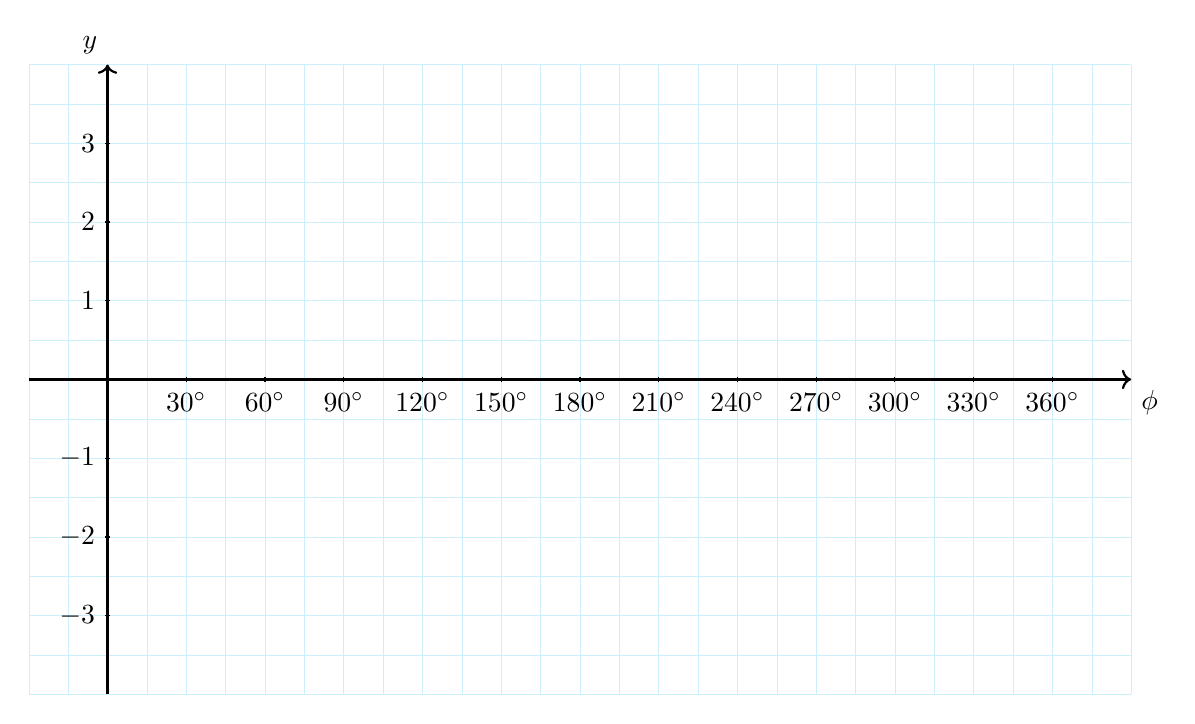
\begin{tikzpicture}
\draw[step = 0.5 cm, cyan!20 , very thin] (-1, -4) grid ( 13, 4);
\draw[thick, ->] (-1,0) -- (13,0) node[anchor = north west] {$\phi$};
\draw[thick, ->] (0,-4) -- (0,4) node[anchor = south east] {$y$};

\foreach \x [evaluate=\x as \degree using int(\x*30)] in {1,...,12}{ 
   \draw (\x cm, 1pt) -- (\x cm, -1pt) node[anchor = north] {$\degree^\circ$};
   }
\foreach \y in {-3,-2,-1,1,2,3}
   \draw (1pt, \y cm) -- (-1pt, \y cm) node[anchor = east] {$\y$};
\end{tikzpicture}}%% END Definition

\newcommand{\trigsysB}{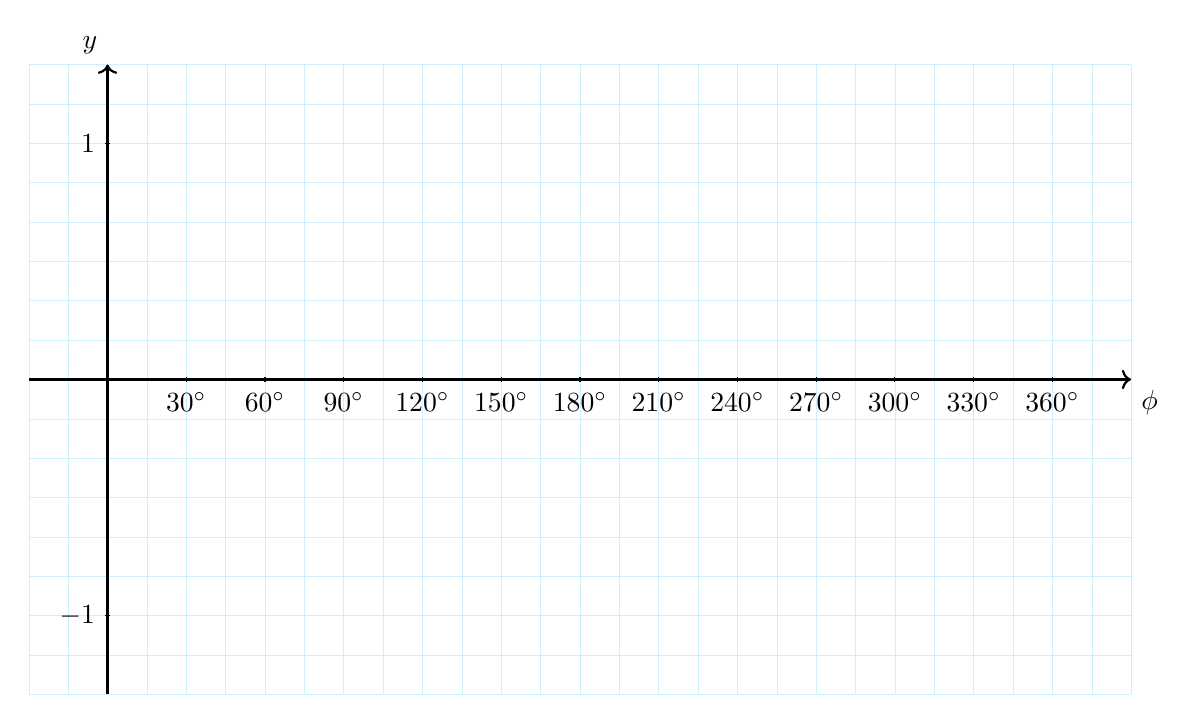
\begin{tikzpicture}\draw[step = 0.5 cm, cyan!20 , very thin] (-1, -4) grid ( 13, 4);
\draw[thick, ->] (-1,0) -- (13,0) node[anchor = north west] {$\phi$};
\draw[thick, ->] (0,-4) -- (0,4) node[anchor = south east] {$y$};

\foreach \x [evaluate=\x as \degree using int(\x*30)] in {1,...,12}{ 
   \draw (\x cm, 1pt) -- (\x cm, -1pt) node[anchor = north] {$\degree^\circ$};
   }
\foreach \y in {-1,1}
   \draw (1pt, \y *3cm) -- (-1pt, \y *3cm) node[anchor = east] {$\y$};

\end{tikzpicture}}%% END Definition

\newcommand{\trigsysC}{
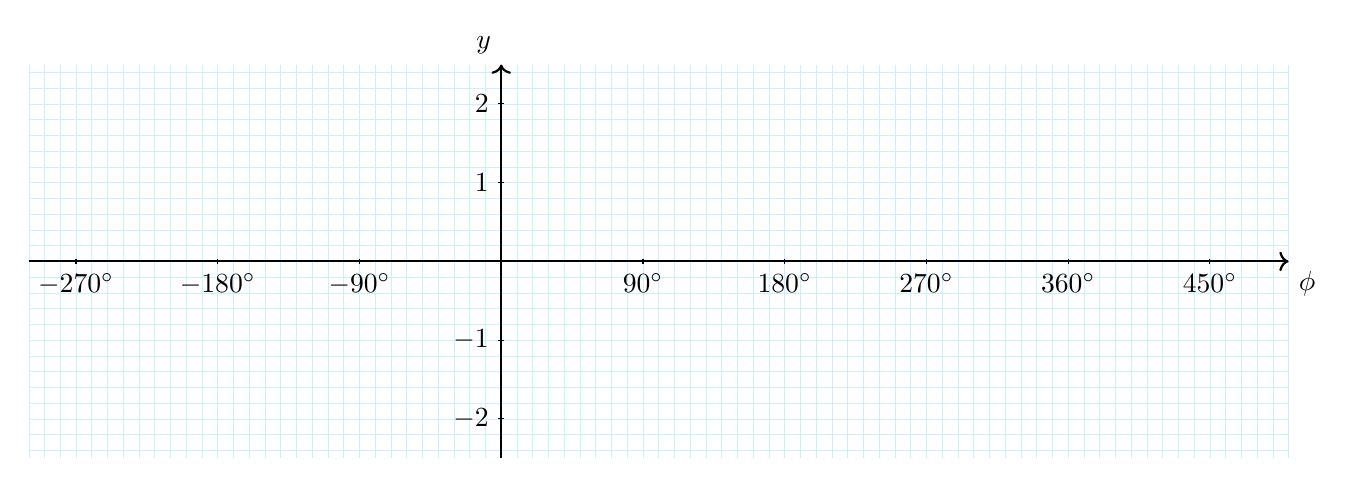
\begin{tikzpicture}
\draw[step = 0.2 cm, very thin, cyan!20] (-6, -2.5) grid ( 10, 2.5);
\draw[thick, ->] (-6,0) -- (10,0) node[anchor = north west] {$\phi$};
\draw[thick, ->] (0,-2.5) -- (0,2.5) node[anchor = south east] {$y$};

\foreach \x [evaluate=\x as \degree using int(\x*90)] in {-3,-2,-1,1,2,3,4,5}{ 
   \draw (\x *18mm, 1pt) -- (\x * 18mm, -1pt) node[anchor = north] {$\degree^\circ$};
   }
   
\foreach \y in {-2,-1,1,2}
   \draw (1pt, \y cm) -- (-1pt, \y cm) node[anchor = east] {$\y$};
\end{tikzpicture}}%% END Definition

\newcommand{\trigsysD}{
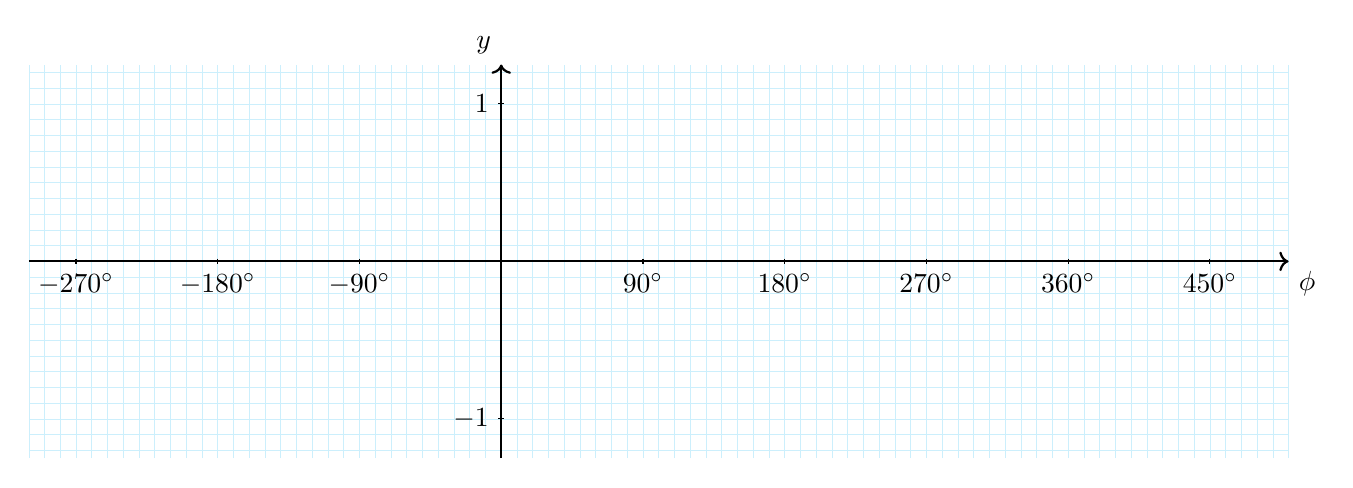
\begin{tikzpicture}
\draw[step = 0.2 cm, very thin, cyan!20] (-6, -2.5) grid ( 10, 2.5);
\draw[thick, ->] (-6,0) -- (10,0) node[anchor = north west] {$\phi$};
\draw[thick, ->] (0,-2.5) -- (0,2.5) node[anchor = south east] {$y$};

\foreach \x [evaluate=\x as \degree using int(\x*90)] in {-3,-2,-1,1,2,3,4,5}{ 
   \draw (\x *18mm, 1pt) -- (\x * 18mm, -1pt) node[anchor = north] {$\degree^\circ$};
   }
   
\foreach \y in {-1,1}
   \draw (1pt, \y *2cm) -- (-1pt, \y *2cm) node[anchor = east] {$\y$};
\end{tikzpicture}}%% END Definition


\newcommand{\trigsysDsin}{
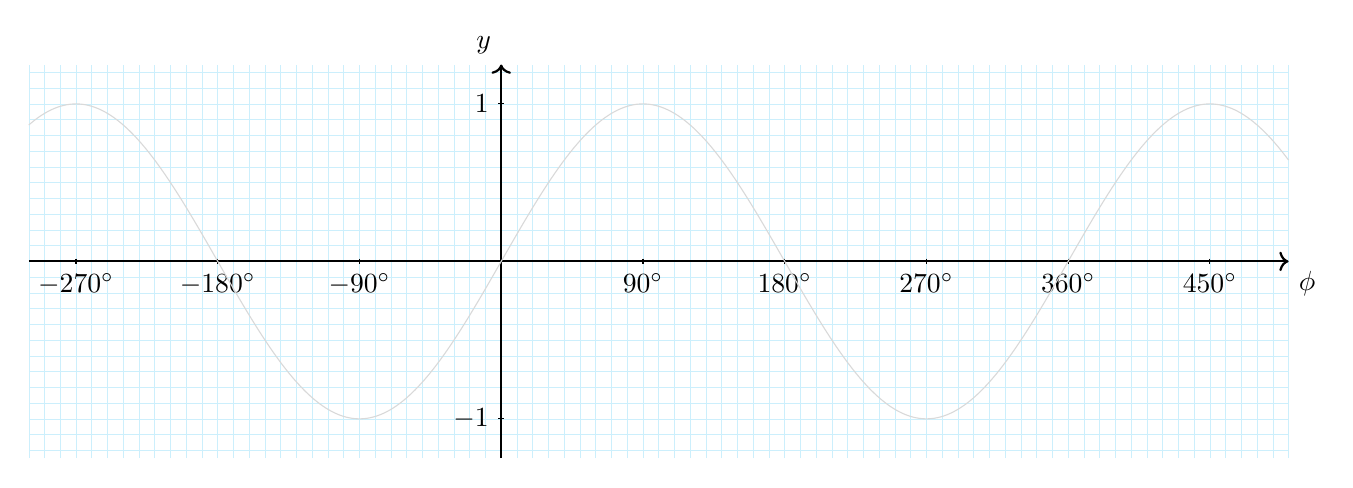
\begin{tikzpicture}
\draw[step = 0.2 cm, very thin, cyan!20] (-6, -2.5) grid ( 10, 2.5);
\draw[thick, ->] (-6,0) -- (10,0) node[anchor = north west] {$\phi$};
\draw[thick, ->] (0,-2.5) -- (0,2.5) node[anchor = south east] {$y$};

\foreach \x [evaluate=\x as \degree using int(\x*90)] in {-3,-2,-1,1,2,3,4,5}{ 
   \draw (\x *18mm, 1pt) -- (\x * 18mm, -1pt) node[anchor = north] {$\degree^\circ$};
   }
   
\foreach \y in {-1,1}
   \draw (1pt, \y *2cm) -- (-1pt, \y *2cm) node[anchor = east] {$\y$};

\draw[domain=-6:10,smooth,samples=200,variable=\x,gray!30] plot ({\x},{2*sin(\x*50)});
\end{tikzpicture}}%% END Definition

\newcommand{\trigsysDcos}{
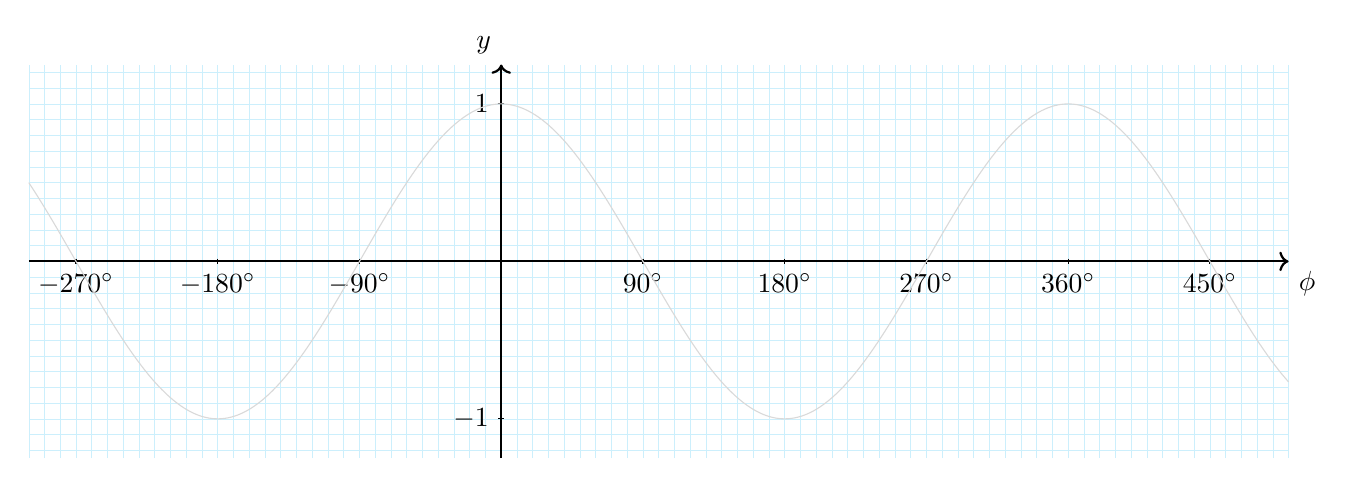
\begin{tikzpicture}
\draw[step = 0.2 cm, very thin, cyan!20] (-6, -2.5) grid ( 10, 2.5);
\draw[thick, ->] (-6,0) -- (10,0) node[anchor = north west] {$\phi$};
\draw[thick, ->] (0,-2.5) -- (0,2.5) node[anchor = south east] {$y$};

\foreach \x [evaluate=\x as \degree using int(\x*90)] in {-3,-2,-1,1,2,3,4,5}{ 
   \draw (\x *18mm, 1pt) -- (\x * 18mm, -1pt) node[anchor = north] {$\degree^\circ$};
   }
   
\foreach \y in {-1,1}
   \draw (1pt, \y *2cm) -- (-1pt, \y *2cm) node[anchor = east] {$\y$};

\draw[domain=-6:10,smooth,samples=200,variable=\x,gray!30] plot ({\x},{2*cos(\x*50)});
\end{tikzpicture}}%% END Definition




\usepackage{bbwLayoutDocSty}

%%%%%%%%%%%%%%%  H E A D E R   &   F O O T E R %%%%%%%%%%%%%%%%%%%%

%% Oben (Header) linke Seite
\fancyhf[HLE]{\makebox{
\includegraphics[width=37mm]{logos/bbwBreit.pdf}}} 
\fancyhf[HCE]{\parttitle}
%% Oben (Header) rechte Seite
\fancyhf[HRO]{\leftmark}
%% Unten (Footer)  FRE = right even, FLE= left even, FRO = right odd,
%% FCO = center odd
\fancyhf[FRE]{\doctitel{}:\ \fachthema}
\fancyhf[FLE,FRO]{\thepage{}/\pageref{LastPage}}
\fancyhf[FCO]{BBW: Abteilung 6 BMS}



\renewcommand{\author}{Philipp G. Freimann}
\renewcommand{\grafikautor}{Ph. G. Freimann}
\renewcommand{\authoremail}{philipp.freimann@bbw.ch}
\renewcommand{\erstellungsdatum}{\versionGESOMajorDate}
\renewcommand{\docversion}{\versionGESOMajorVSR}

%%\renewcommand{\modulnummer}{Arithmetik und Algebra I}
\renewcommand{\doctitel}{Mathematik}
\renewcommand{\fachthema}{3jährige BM1}

%% Gesamt-Skripts benötigen ALINONE (all in one), damit Referenzen auf andere
%% Kapitel funktioniren:
\isALLINONEtrue%%

\scriptStart{}

%% EinstiegsAufgaben
%%
%% 2019 07 04 Ph. G. Freimann
%%

\section*{Einstiegsaufgaben}
\sectuntertitel{Der Anfang ist die Hälfte des Ganzen (Aristoteles)}
%%%%%%%%%%%%%%%%%%%%%%%%%%%%%%%%%%%%%%%%%%%%%%%%%%%%%%%%%%%%%%%%%%%%%%%%%%%%%%%%%
\GESO{\cite{marthaler21} ab. S. 22}


\subsection*{Abholen des Bekannten und Geübten}

\GESO{
  
  Vereinfachen Sie den Term so weit wie möglich\footnote{Aufgaben aus
    BMS Aufnahmeprüfungen}:
  $$\sqrt{(7x)^2 + 17x^2 - 2x^2}$$

\TNT{3.2}{
  $$\sqrt{49x^2 + 17x^2 - 2x^2}$$
  $$\sqrt{64x^2} = 8x$$
  \vspace{3cm}} %% END TNT

  %%%%%%%%%%%%%%%%%%%%%%%%%%%%%%%%%%55

  Berechnen Sie die Lösung der Gleichung:

  $$x^2 + 11 = (x+3)^2$$

\TNT{7.2}{$$x = \frac{1}{3}$$
\vspace{5cm}
  }


    %%%%%%%%%%%%%%%%%%%%%%%%%%%%%%%%%%55
  \newpage
  Vereinfachen Sie den Term so weit wie möglich:

  $$\frac{4b^2}{2a}:\frac{b^2}{3a^2} - \frac{a}{5}$$

\TNT{7.2}{$$\frac{4b^2}{2a}\cdot{}\frac{3a^2}{b^2} - \frac{a}{5}$$
    $$\frac{4\cdot{}3a}{2} - \frac{a}{5}$$
    $$\frac{60\cdot{}a}{10} - \frac{2a}{10}$$
    $$\frac{58a}{10} = 5.8a$$
\vspace{5cm}
  
}
  \newpage


In einer Schachtel liegen vier grüne und fünf rote Kugeln.
Sie ziehen nacheinander zwei Kugeln, ohne sie wieder zurückzulegen.

a) Zeichnen Sie einen entsprechenden Wahrscheinlichkeitsbaum und tragen Sie die
Wahrscheinlichkeiten bei den Ästen ein.

\TNT{4.8}{\vspace{48mm}}


b) Berechnen Sie die Wahrscheinlichkeit, zwei grüne Kugeln zu ziehen.

\TNT{4.8}{\vspace{48mm}}

%%%%%%%%%%%%%%%%%%%%%%%%%%%%%%%%%%%%%%%%%%%%%%%5
%  Ein Radfahrer fährt von zu Hause zum Arbeitsplatz. Am Anfang fährt
%  er während 15 Minuten mit einer Geschwindigkeit von 30 km/h. An
%  einer Ampel muss er für 3 Minuten anhalten. Anschließend fährt er
%  während 30 Minuten mit einer Geschwindigkeit von 20 km/h bis zum
%  Arbeitsplatz.

%  Was ist die durchschnittliche Geschwindigkeit des Radfahrers von
%  seinem Wohnort bis zur Arbeit in km/h?

%\noTRAINER{  \mmPapier{8.0}}
%  \TRAINER{1. Totale Strecke rechnen (17.5 km). 2. Totale Zeit
%    rechnen: 48 Minuten = 0.8 h. Danach: v = s/t: 21.875km/h.
%    \vspace{5cm}}

}%% END GESO
\newpage


%% Arithmetik und Algebra
%%
%% GESO Metapackeg Arithmetik und Algebra II

%%%%%%%%%%%%%%%%
\part{Arithmetik und Algebra II}\index{Arithmetik und Algebra!II|textbf}
\renewcommand{\bbwPartID}{AA2}
%%
%% 2019 07 04 Ph. G. Freimann
%%

\section{Potenzen}\index{Potenzen}
\sectuntertitel{Ein dreifaches Hoch auf die Basen}

\theorieGESO{57-59}{4.1, 4.2, 4.3 und 4.4}

%%%%%%%%%%%%%%%%%%%%%%%%%%%%%%%%%%%%%%%%%%%%%%%%%%%%%%%%%%%%%%%%%%%%%%%%%%%%%%%%%
\subsection*{Lernziele}

\begin{itemize}
\item Definition: Exponent, Basis, Potenz
\item Rechengesetze
\item Hoch 0
\item negative Exponenten
\item Potenzen von Bruchtermen
\item Namen der Zehnerpotenzen
\end{itemize}
\TALS{(\cite{frommenwiler17alg} S. 32 (Kap. 1.5))}
\newpage
%%\subsection{Definition}
%%$$a^n = \underbrace{a\cdot a \cdot a \cdot ... \cdot a}_{\textrm{n Faktoren}}$$


\subsection{Zehnerpotenzen}\index{Zehnerpotenzen}
\TadBMTA{61}{4.5}

\bbwCenterGraphic{8cm}{allg/alg/potenzen_wurzeln/img/one_in_a_mellon.jpg}

Neben den im Buch (\cite{marthaler21alg} S. 62) angegebenen SI-Einheiten (Kilo, Mega, ...) sind die
Namen der positiven Zehnerpotenzen im Englischen anders als im
Deutschen. Hier zur Vollständigkeit:

\begin{tabular}{lrclll}
Potenz    & Zahl & SI-Kürzel & SI-Vorsätze & Deutsch & Englisch\\
\hline\\
$10^{2}$   & 100  & h         & Hekto       & Hundert   & hundred\\
$10^{3}$   & 1000 & k         & Kilo        & Tausend   & thousand\\
$10^{6}$   & ...  & M         & Mega        & Million   & million\\
$10^{9}$   & ...  & G         & Giga        & Milliarde & billion\\
$10^{12}$  & ...  & T         & Tera        & Billion   & trillion\\
$10^{15}$  & ...  & P         & Peta        & Billiarde & quadrillion\\
$10^{18}$  & ...  & E         & Exa         & Trillion  & quintillion\\
\end{tabular}

\begin{tabular}{lrclll}
Potenz     & Zahl & SI-Kürzel & SI-Vorsätze & Deutsch\\
\hline\\
$10^{-1}$  & 0.1   & d         & Dezi        & Zehntel\\
$10^{-2}$  & 0.01  & c         & Centi       & Hundertstel\\
$10^{-3}$  & 0.001 & m         & Milli       & Tausendstel\\
$10^{-6}$  & ...   & $\mu$     & Mikro       & Millionstel\\
$10^{-9}$  & ...   & n         & Nano        & Milliardstel\\
\end{tabular}

Mit dem Taschenrechner können große Zehnerpotenzen mit der
  \GESO{\tiprobutton{EE}}\TALS{\nspirebutton{EE}}-Taste eingegben
  werden: 0.37 Milliarden:

  \GESO{\tiprobutton{0}\tiprobutton{dot}\tiprobutton{3}\tiprobutton{7}\tiprobutton{EE}\tiprobutton{9}}%% END GESO
  \TALS{\nspirebutton{0}\nspirebutton{dot}\nspirebutton{3}\nspirebutton{7}\nspirebutton{EE}\nspirebutton{9}}%% END TALS


\newpage


\subsubsection{Ausklammern von Zehnerpotenzen}
Gegeben ist die folgende Summe. Leider etwas mühsam zum Lesen wegen der vielen Nullen. Klammern Sie tausend (= $10^3$) aus:

$$400\,000 + 5\,000 + 3\,000\,000 + 70$$
\TNT{3.2}{
$$ = 4\cdot{} 10^5 + 5\cdot{} 10^3 + 3\cdot{} 10^6 + 7\cdot{} 10^1$$
$$ = 10^3 \cdot{} (4\cdot{}10^2 + 5 \cdot{} 1 + 3\cdot{} 10^3 + 7
  \cdot{} 0.01)$$
  $$=10^3\cdot{} (400 + 5 + 3000 + 0.07)  $$
  $$= (3405.07 \cdot{} 10^3) = 3405.07 k$$
}%% END TNT


\paragraph{Ausklammern negativer Zehnerpotenzen:}
\,

\vspace{1mm}

Genauso, wie man positive Zehnerpotenzen ausklammern kann, kann man auch negative Zehnerpotenzen ausklammern. Dies ist insofern praktisch, um sich einen Überblick zu verschaffen, bei sehr kleinen positiven Größen:

Klammern Sie einen Millionstel (=$10^{-6}$) aus:


$$a\cdot{}10^{-6} + b\cdot{}10^{-2} + c\cdot{}10^{-5} +
d\cdot{}10^{-1} = \LoesungsRaumLang{(a + b\cdot{}10^4 + 10c + d\cdot{}10^{5}) \cdot{} 10^{-6}}$$

\subsection*{Aufgaben}

%%\TALS{Zehnerpotenzen:}
%%\TALSAadBMTA{41ff}{110. a) b) c) d), 111. c) f), 112. a) d) e) f) m) 114. und 116.}
%%\TALS{Zehnerpotenzen ausklammern:}
%%\TALSAadBMTA{34}{88. e) und h)}

%%  \AadBMTA{65ff}{3. b) c), 4. c), 12. und 16. a) und c)}
%%  \AadBMTA{68ff}{24. c), 28. c)}
%%  \AadBMTA{74ff}{52. a) c) d), \GESO{ (optional) }53. a) b) d) h) i), 57. a) b) e)}
%%  \AadBMTA{75}{60., 63. und 64.}


\GESO{\olatLinkArbeitsblatt{Potenzgesetze}{https://olat.bbw.ch/auth/RepositoryEntry/572162163/CourseNode/102690264435484}{Kapitel
    1 (Aufgaben 1. - 16.)}}%% END olatLinkArbeitsblatt
\TALS{\olatLinkArbeitsblatt{Potenzgesetze}{https://olat.bbw.ch/auth/RepositoryEntry/572162090/CourseNode/104915210426569}{Kapitel
    1 (Aufgaben 1. - 16.)}}%% END olatLinkArbeitsblatt

\newpage


\input{bbwLayoutPage}
\renewcommand{\bbwAufgabenBlockID}{APot}


%%%%%%%%%%%%%%%%%%%%%%%%%%%%%%%%%%%%%%%%%%%%%%%%%%%%%%%%%%%%%%%%%%

\usepackage{amssymb} %% für \blacktriangleright
\renewcommand{\metaHeaderLine}{Potenzgesetze}
\renewcommand{\arbeitsblattTitel}{(BMS Version 1.1)}

\begin{document}%%
\arbeitsblattHeader{}


%\newcounter{aufgabennummer}
%\setcounter{aufgabennummer}{1}

\newcommand\aufgabeML[3]{

Aufgabe \arabic{bbwAufgabenNummerCounter}. :\,\,
$${#2}$$ = $\LoesungsRaum{{#3}}$

\abplz{#1}

\stepcounter{bbwAufgabenNummerCounter}
}

{\huge{Vermischte Aufgaben zu Potenzgesetzen}}


\section{Zehnerpotenzen}

Berechnen Sie Zehnerpotenzen und vergleichen Sie:

\aufgabeML{6}{(-10)^4}{10\,000}
\aufgabeML{6}{-10^4}{-10\,000}


\aufgabeML{6}{(-10)^5}{-100\,000}
\aufgabeML{6}{-10^7}{-10\,000\,000}
\aufgabeML{6}{(-10)^8}{+100\,000\,000}
\aufgabeML{6}{-(10^6)}{-1\,000\,000}


\aufgabeML{6}{0.1^1}{0.1}
\aufgabeML{6}{0.1^2}{0.01}
\aufgabeML{6}{-0.1^4}{-(0.1^4) = -0.0001}
\newpage

Aufgabe \arabic{bbwAufgabenNummerCounter}.: 
Füllen Sie die Tabelle aus. Tipp: Welche Operation wird in den
hinteren drei Spalten konsequent von einer Zeile zur nächsten ausgeführt?

\begin{bbwFillInTabular}{|r|r|r|l|}\hline
Exponent       & Zehnerpotenz & Potenzwert & Name \\\hline
$4$            &  $10^4$           &  $10\,000$        & Zehntausend         \\\hline
$3$            &  \TRAINER{$10^3$} &  \TRAINER{$1000$} & \TRAINER{Tausend}   \\\hline
$2$            &  \TRAINER{$10^2$} &  \TRAINER{$100$}  & \TRAINER{Hundert}   \\\hline
$\TRAINER{1}$  &  \TRAINER{$10^1$} &  \TRAINER{$10$}   & \TRAINER{Zehn}      \\\hline
$\TRAINER{0}$  &  \TRAINER{$10^0$} &  \TRAINER{$1$}    & \TRAINER{Eins}      \\\hline
$\TRAINER{-1}$ &  \TRAINER{$10^{-1}$} &  \TRAINER{$0.1$}  & \TRAINER{Ein Zehntel}      \\\hline
$-2$           &  \TRAINER{$10^{-2}$} &  \TRAINER{$0.01$}	 & \TRAINER{Ein Hundertstel}      \\\hline
\end{bbwFillInTabular}
\stepcounter{bbwAufgabenNummerCounter}


Schreiben Sie ohne Klammern und ohne Bruchstrich:
\aufgabeML{6}{\frac1{10\,000}}{10^{-4}}

Fassen Sie die Zehnerpotenzen zusammen und schreiben Sie
wissenschaftlich (genau eine Ziffer vor dem Dezimalpunkt):

\aufgabeML{6}{9\cdot{}10^3 + 4.7 \cdot{}10^4}{5.6\cdot{} 10^4}
\aufgabeML{6}{2\cdot{}10^{-4} + 220.3 \cdot{} 10^-5}{2.403 \cdot{} 10^{-3}}



Multiplizieren Sie die Zehnerpotenzen (gleiche Basis):
\aufgabeML{6}{-0.1^4\cdot{} 0.1^5}{-0.1^{9} = -0.000\,000\,001}

\arabic{bbwAufgabenNummerCounter}.:
Ein rotes Blutkörperchen hat ein Gewicht von $3\cdot{}10^{-11}$ g.
Beim Menschen liegt die Konzentration im Blut bei $4\,000$ bis $5\,900$ Stück pro Nanoliter.

\begin{bbwAufgabenBlock}
\item Geben Sie die Anzahl der roten Blutkörperchen je im Minimum und
im Maximum pro Liter Blut mit Hilfe von Zehnerpotenzen
an.\TRAINER{Minimal: $4000\cdot{}10^9 = 4\cdot{}10^{12}$, maximal:
$5.9\cdot{}10^{12}$}

\item Wie viele solcher Blutkörperchen hat ein Mensch, wenn wir von
einer Konzentration von 5\,000 Stück pro Nanoliter ausgehen und von
einer Blutmenge von 6 Litern? Wie heißt die Zahl in Worten?
\TRAINER{$6\cdot{} 5.0\cdot{}10^{}12 = 3.0 \cdot{} 10^{13}$ = 30
Billionen}

\item Wie groß ist die Masse aller roten Blutkörperchen einer Person,
wenn wir von 6 Liter Blut und 5\,000 roten Blutkörperchen pro
Nanoliter ausgehen?
\TRAINER{$3.0\cdot{}10^{13} \cdot{} 3\cdot{} 10^{-11} \text{ g } = 9\cdot{}10^2 \text{ g } = 900 \text{ g }$}
\end{bbwAufgabenBlock}

%%%%%%%%%%%%%%%%%%%%%%%%%%%%%%%%%%%%%%%%%%%%%%%%%%%%%%%%%%%%%%%%%%%%%%%%%%%%%%%%%%%%%%%%%%%%%%%%%%

\section{Ganze positive Exponenten}

\aufgabeML{6}{-\left((-a)^3\right)^{10}}{-a^{30}}\noTRAINER{\newpage}

\aufgabeML{6}{\left(-(-x^2)\right)^7}{x^{14}}


\aufgabeML{6}{\left(-x^3\right)^4}{x^{12}}
%%\platzFuerBerechnungenBisEndeSeite{}

\newpage
\section{Division}

\aufgabeML{6}{c^9 : c^4}{c^5}

\aufgabeML{6}{\frac{a^2}{a^3}}{\frac{1}{a}=a^{-1}}\noTRAINER{\newpage}

\aufgabeML{6}{(-a)^4:(-a^{10})}{-\frac{1}{a^6}}

\aufgabeML{6}{a\cdot{} a^{2x+3} : a^{1-x}}{a^{3x+3}}\noTRAINER{\newpage}

\aufgabeML{6}{\left(\frac{x}{y}\right)^7:\left(\frac{-x}{y}\right)^3}{-\left(\frac{x}{y}\right)^4}\noTRAINER{\newpage}

\newpage
\section{negative Exponenten und die Null}

\aufgabeML{6}{-\left(-(-a)^2\right)^0}{-1}

\aufgabeML{6}{-\left( -a^3\cdot{} (-a)^2 \right)^{-4}}{\frac{-1}{a^{20}} = -a^{-20}}\noTRAINER{\newpage}

\aufgabeML{6}{(-b)^{-6} \cdot (-b^8)}{-b^2}

\aufgabeML{6}{\left(-(a^{-1})^{-2}\right)^6}{a^{12}}\noTRAINER{\newpage}

\aufgabeML{6}{-\left((a^3)\cdot{}a^{-1}\right)^2}{-a^4}
\noTRAINER{\newpage}

Schreiben Sie ohne negative Exponenten:

\aufgabeML{6}{2\cdot{}x^{-3}}{\frac{2}{x^3}}

\aufgabeML{6}{ab^{-5}}{\frac{a}{b^5}=a\cdot{}\frac{1}{b^5}}\noTRAINER{\newpage}

\aufgabeML{6}{\frac{1}{81}\cdot{}c^{-2}\cdot{}a^{-3}\cdot{}c^2\cdot{} a^3 \cdot 3^4}{1}
%%\platzFuerBerechnungenBisEndeSeite{}

\newpage
\section{negative Exponenten mit Brüchen}
\aufgabeML{6}{\frac{6\cdot{} a^3 \cdot{} b^7 \cdot{} 3}{(ab)^4\cdot 9 \cdot a^{-1}}}{2b^3}

\aufgabeML{6}{\left(\frac{a^2 b^{-3} c^3}{a\cdot b}\right)^{-3}\cdot \left(\frac{c^5}{ab}\right)^2}{\frac{b^{10}c}{a^5}}\noTRAINER{\newpage}

\aufgabeML{6}{\left(\frac{ab^{-2}c^3}{a^{-2}\cdot{}b}\right)^{-2} \cdot{} \left(\frac{a^3\cdot{} c^{2}}{b^2} \right)^3}{a^3}


\aufgabeML{6}{\left(\frac{a^3 \cdot{}c^{-1}}{b^{-2}}\right)^{-4} \cdot \left( \frac{a^4\cdot{}b^3}{c^{-2}} \right)^3}{bc^{10}}\noTRAINER{\newpage}

\aufgabeML{6}{\frac{a^{-5}\cdot{} (-a)^3}{a^7} : \frac{a^{-10}}{a^4} }{-a^5}

\aufgabeML{6}{\frac{ab\cdot{}b^{-2}\cdot{}b^4\cdot{}b^{-3}}{b^3\cdot{}a\cdot{}b^{-4} \cdot{} b}}{1}\noTRAINER{\newpage}


\aufgabeML{6}{\left(\frac{3x^{-2}y^2}{4x^{-4}\cdot{}y^3}\right)^{-2} : \left(\frac{2x^{-1}}{3xy^{-2}}\right)^3}{\frac{6x^2}{y^4}}

\aufgabeML{6}{4^k\cdot{} \left(\frac{1}{2}\right)^k \cdot{} \left(\frac{1}{3}\right)^{-k}}{6^k}\noTRAINER{\newpage}

\aufgabeML{6}{\frac{a^{-2}}{a^{-3}}}{a}

\aufgabeML{6}{\left(\frac{a^4\cdot{}b^{-2}\cdot{}c}{a^2\cdot{}c^{-3}}\right)^{-2} \cdot \left(\frac{c^2\cdot{}b}{a^{-1}}\right)^4}{b^8}\noTRAINER{\newpage}


\aufgabeML{6}{\left(\frac{3a^{-1}\cdot{} b^2}{2ac^{-1}}\right)^{-2} \cdot{} \frac{\left(3\cdot{}b^2\right)^2\cdot{}c^2}{4}}{a^4}

\aufgabeML{6}{a^{-1}\cdot{} a^{-2} : a^{-3} \cdot{} a^7}{a^7}\noTRAINER{\newpage}

\newpage
\section{Wurzeln}

\aufgabeML{6}{\sqrt{a^2}}{a}

\aufgabeML{6}{\left(\sqrt[2]{x}\right)^2}{x}\noTRAINER{\newpage}

\aufgabeML{6}{\sqrt[3]{b^3}}{b}

\aufgabeML{6}{\sqrt[3]{z^9}}{z^3}\noTRAINER{\newpage}

\aufgabeML{6}{\sqrt[5]{b^{10}r^5}}{b^2r}

\aufgabeML{6}{\sqrt[4]{r^8n^{12}}}{r^2n^3}\noTRAINER{\newpage}

\aufgabeML{6}{\sqrt[5]{m^4\cdot{m}}}{m}

\aufgabeML{6}{\sqrt{m^2+m^2 + m^2}}{\sqrt{3}\cdot{}m}\noTRAINER{\newpage}

\aufgabeML{6}{\sqrt{\sqrt[2]{x^4}}}{x}

\aufgabeML{6}{\frac{\sqrt[3]{a^7}}{\sqrt[3]{a}}}{a^2}\noTRAINER{\newpage}

\aufgabeML{6}{\sqrt[8]{r^{24}}}{r^3}
\noTRAINER{\newpage}

Und als Überleitung ins nächste Thema:

\aufgabeML{6}{\sqrt[6]{v^3}}{v^{\frac12} = \sqrt{v}}



\newpage
\section{Rationale Exponenten}

\aufgabeML{6}{a^4\cdot{}a^{\frac{1}{4}}\cdot a^5\cdot a^{\frac{-1}{5}}}{a^\frac{181}{20}}

\aufgabeML{6}{\sqrt[4]{a^3}}{a^{\frac{3}{4}}}\noTRAINER{\newpage}

\aufgabeML{6}{\sqrt[3]{r^{\frac{3}{4}}}}{\sqrt[4]{r} = r^{\frac{1}{4}}}

\aufgabeML{6}{\sqrt{b^\frac12}}{\sqrt[4]b = b^\frac14}\noTRAINER{\newpage}

\aufgabeML{6}{\sqrt{a^\frac{1}{2}} \cdot \sqrt[4]{a\cdot{} \sqrt[5]{a^{10}}}}{a}

\aufgabeML{6}{\sqrt{x^{10}} \cdot \sqrt[4]{x^3} \cdot x^{\frac{1}{4}}}{x^6}\noTRAINER{\newpage}

\aufgabeML{6}{\sqrt[3]{a} \cdot \sqrt{a^3 \cdot \sqrt[3]{a}}}{a^2}

\aufgabeML{6}{\sqrt[3]{a^2} \cdot \sqrt[4]{a^3 \cdot \sqrt[3]{a}}}{a^{\frac{9}{6}} = \sqrt[6]{a^9} = a^\frac32 = \sqrt{a^3}}\noTRAINER{\newpage}

\aufgabeML{6}{\sqrt[3]{b\cdot \sqrt{b^3\cdot \sqrt[3]b}}}{\sqrt[9]{b^8}}

\aufgabeML{6}{\sqrt[4]{b\cdot{} \sqrt[3]{b^2\cdot \sqrt{b}}}}{b^\frac{11}{24} = \sqrt[24]{b^{11}}}\noTRAINER{\newpage}

\aufgabeML{6}{3a\cdot \sqrt[3]{9a^2}}{\sqrt[3]{3^5 a^5} = \left(3a\right)^\frac53}

\aufgabeML{6}{\sqrt{x} \cdot \sqrt[3]{x^4} \cdot \sqrt[6]{x^3}}{x^\frac73 = \sqrt[3]{x^7}}\noTRAINER{\newpage}

\aufgabeML{6}{\sqrt{a^3}\cdot \sqrt[3]{a^2}}{a^\frac{13}{6} = \sqrt[6]{a^{13}}}

\aufgabeML{6}{\sqrt{a^2 \sqrt{a}}}{a^\frac54 = \sqrt[4]{a^5}}\noTRAINER{\newpage}

\aufgabeML{6}{\sqrt{a^{-2}}}{\frac{1}{a} = a^{-1}}

\aufgabeML{6}{\sqrt[3]{a^2 \cdot b \cdot \sqrt{a\cdot b^{-1}}}}{a^\frac56 \cdot b^\frac16 = \sqrt[6]{a^5\cdot b}}\noTRAINER{\newpage}

\aufgabeML{6}{\sqrt{x^3} \cdot \left(\sqrt{x}\right)^{-3}}{1}

\aufgabeML{6}{\frac{\sqrt{a^3}}{\sqrt{a^{-1}}}}{a^2}\noTRAINER{\newpage}

\aufgabeML{6}{\left(\frac{1}{a}\right)^{-\frac14}}{\sqrt[4]a = a^\frac14}

\aufgabeML{6}{\frac{a^4}{\sqrt{a}}}{\sqrt{a^7} = (\sqrt{a})^7 = a^\frac72}\noTRAINER{\newpage}

\aufgabeML{6}{\frac{\sqrt[3]{a^2}}{\sqrt{a}}}{a^{\frac16} = \sqrt[6]{a}}

\aufgabeML{6}{\frac{-\sqrt{a^3}}{-\left(\sqrt{a}\right)^3}}{1}\noTRAINER{\newpage}

\aufgabeML{6}{\frac{\sqrt[3]{a^{13}}}{a^4}}{a^{\frac13} = \sqrt[3]{a}}


\aufgabeML{6}{\sqrt[3]{26\cdot{} \sqrt[4]{a^3} + \sqrt[8]{a^6}}}{3\cdot{}\sqrt[4]{a}}
%%\platzFuerBerechnungenBisEndeSeite{}

\end{document}


\subsubsection{Negative Exponenten}
\sectuntertitel{Nicht für alle ist die Potenzrechnung \textit{positiv}.}
Wir kennen bereits das Rechengesetz für positive Exponenten:

$$a^5\cdot{}a^2 = a^{5+2} = a^7$$

Sinnvoll wäre die folgende Erweiterung auf negative
Exponenten:\\\TRAINER{Damit die Rechengesetze weiterhin gelten.}
$$a^5\cdot{}a^{-2} = a^{5+(-2)} = a^3$$

Dividieren wir obige Gleichung beidseitig durch $a^5$, so erhalten wir
folgende sinnvolle Definition:

\TNT{6}{

$$a^5\cdot{} a^{-2} = a^3$$

Wir dividieren beidseitig durch $a^5$:

$$\frac{a^5\cdot{}a^{-2}}{a^5} = \frac{a^3}{a^5}$$

$$a^{-2} = \frac{a^3}{a^5} = \frac{1}{a^2}$$

Damit ist die folgende Definition sinnvoll: 
}%% END TNT

\begin{definition}{}{}
$$a^{-n} := \frac{1}{a^n}$$
\end{definition}

\begin{bemerkung}{}{}
$$ a^{-n} =\frac1{a^n}= 1 : \underbrace{a : a : a : ... : a}_{n \text{\ Divisoren}}$$
\end{bemerkung}

\begin{gesetz}{}{}
$a^{-n} = \left(\frac1a\right)^n$
\end{gesetz}
Begründung:

\TNTeop{$a^{-n} = \frac1{a^n}
= \frac1{\underbrace{a\cdot{}a\cdot{}a\cdot{}...\cdot{}a}_{n \text{\ Faktoren}}}
= \underbrace{\frac1a\cdot{}\frac1a\cdot{}\frac1a\cdot{}...\cdot{}\frac1a}_{n \text{\ Faktoren}}
= \left(\frac1a\right)^n$
}%% END TNT

%%%%%%%%%%%%%%%%%%%%%%%%%%%%%%%%%%%%%%%%%%%%%%%%%%%%%%

Ganz analog gilt:
\TRAINER{Lieblingsgesetz von $\varphi$: Wer mag negative Exponenten?
Wer mag Brüche?}

\begin{gesetz}{}{}
$\frac{1}{a^{-n}} = \LoesungsRaumLen{30mm}{a^n}$
\end{gesetz}
Begründung:
\TNT{8}{

Beispiel:

$$\frac1{10^{-3}} = \frac1{0.001} = 1000 = 10^3$$

\TALS{TALS:}
Beweis: Definition hinschreiben und auf beiden Seiten den Kehrwert bilden:

$$a^{-n} = \frac1{a^n}$$

$$\frac1{a^{-n}} = a^n$$

\vspace{2cm}
}%% END TNT



\begin{gesetz}{}{}
$\left(\frac{1}{a}\right)^{-n}=\LoesungsRaumLen{30mm}{a^n}$
\end{gesetz}
Begründung:
\TNTeop{
Zahlenbeispiel (erster Schritt nach Definition):
$$\left(\frac1{10}\right)^{-3}  = \frac1{\left(\frac1{10}\right)^3}  = \frac1{0.001} = 1000 = 10^3$$

\TALS{TALS:}

Beweis: Nach Definition gilt:

$$x^{-n} = \frac1{x^n}$$

Somit gilt es auch, wenn wir anstelle von $x$ den Term $\frac1a$ einsetzen:

$$\left(\frac1a\right)^{-n} = \frac{1}{\left(\frac{1}{a}\right)^n}
= \frac1{\frac1{a^n}} = 1 : \frac{1}{a^n}= 1\cdot{}\frac{a^n}{1}=a^n$$


\vspace{2cm}

}%% END TNT

%%%%%%%%%%%%%%%%%%%%%%%%%%%%%%%%%%%%%%


Rechenbeispiel\GESO{ (optional)}:

Wurm «Wurli» schaft 3 cm pro Sekunde (= $3 \cdot{} 10^{-2} $ m pro Sekunde). Wie lange braucht «Wurli» für 12 m?
\TNT{4}{
$$t = \frac{s}v
= \frac{12[ \text{m}]}{3 \frac{[\text{cm}]}{[\text{s}]}}
= \frac{12[ \text{m}]}{3\cdot{}10^{-2}\frac{[\text{m}]}{[\text{s}]}}= \frac{4[ \text{m}]}{10^{-2}\frac{[\text{m}]}{[\text{s}]}}
= 4\cdot{} 10^2 [\text{s}]
= 400 [\text{s}]
\approx 6-7 \text{ Min.}$$

\vspace{28mm}
}%% END TNT




Und ebenso für beliebige Brüche:

\begin{gesetz}{}{}
$\left(\frac{a}{b}\right)^{-n} = \left(\frac{b}{a}\right)^{+n}$
\end{gesetz}

    
    \TALS{ Begründung

      \TNT{2.4}{
$\left( \frac{a}{b} \right)^{-n}  =
 \left(a \cdot{} \frac{1}{b} \right)^{-n} =
 b^{-n} \cdot \left(\frac{1}{a}\right)^{-n} =
 \left(\frac{1}{b}\right)^{n} \cdot{} a^{n} =
 \left(\frac{1}{b}\cdot{}a\right)^{n} =
 \left(\frac{a}{b}\right)^{n} $}} %% END TNT END TALS

    \GESO{ Begründung

      \TNT{2.4}{$\left( \frac{5}{2} \right)^3  =
       \left(5 \cdot{} \frac{1}{2} \right)^3 =
       5^3 \cdot \left(\frac{1}{2}\right)^3 =
       \left(\frac{1}{5}\right)^{-3} \cdot{} 2^{-3} =
       \left(\frac{1}{5}\cdot{}2\right)^{-3} =
       \left(\frac{2}{5}\right)^{-3} 
       $}} %% END TNT END GESO

%%$$\left(\frac{1}{a}\right)^{-n} = \frac{1}{\left(\frac{1}{a}\right)^n} = a^n$$
\newpage



\subsubsection{Null}

Idee:
\TNT{3.2}{$$a^5\cdot{}a^0 \stackrel{!}{=} a^{5+0} = a^5$$
$$a^5 \cdot{} a^0 \stackrel{!}{=} a^5   \hspace{5mm} | : a^5$$
$$a^0 = 1$$
}%% end TNT

Oder so:
\TNT{3.2}{
$$a^0 = a^{1-1} = a^1 : a^1 = a:a = 1$$
}%% end TNT

\begin{definition}{Exponent Null}{} Für alle Basen
$a \in \mathbb{R}\backslash\{0\}$ definieren wir:
\begin{center}
\fbox{$a^0 := 1$}
\end{center}
\end{definition}



%\textbf{Rechengesetze zusammengefasst:}

%\begin{itemize}
%\item  $\frac{a^m}{a^n} = a^{m-n}$ (Dies gilt auch wenn $n > m$.)
 
%\item $a^{-n} := a^{0-n}=\frac{a^0}{a^n} = \frac{1}{a^n} = \left(\frac{1}{a}\right)^n$

%\item
%$\left(\frac{1}{a}\right)^{-n} = \frac{1}{\left(\frac{1}{a}\right)^n} = a^n$


%\item $\left(\frac{a}{b}\right)^{-n} = \left(\frac{b}{a}\right)^{+n}$ gilt daher auch. 
%\end{itemize}


\subsection*{Aufgaben}
\GESO{\olatLinkArbeitsblatt{Potenzgesetze}{https://olat.bms-w.ch/auth/RepositoryEntry/6029794/CourseNode/102690264435484}{Kapitel
    3 Aufg. 56. - 59., 61., 63., 64. - 68.  }}%% END olatLinkArbeitsblatt
\TALS{\olatLinkArbeitsblatt{Potenzgesetze}{https://olat.bms-w.ch/auth/RepositoryEntry/6029786/CourseNode/104915210426569}{Kapitel
    3 Aufg. 56. - 59., 61., 63., 64. - 68.}}%% END olatLinkArbeitsblatt

\newpage

\begin{rezept*}{«Kielholen»}{}{}
Exponenten vertauschen ihr Vorzeichen beim Übertreten des Bruchstrichs:
$$\frac{a^{-3}b^2}{c^5b^{-6}} = \LoesungsRaumLang{\frac{b^2\cdot{}b^{+6}}{a^{+3}c^5}}= \LoesungsRaumLang{\frac{b^8}{a^3c^5}}$$
\end{rezept*}



\subsection{Aufgaben}

%%\TALS{Potenzen:}\TALSAadBMTA{32ff}{Von Hand: 79. c), 82. a), 83. b),
%%86. b) c),
%%91. a), 92. j), 94. k), 96. b) f) h) und 105. i)\\
%%Prüfen Sie die folgenden Aufgaben auch mit dem TR (Training):\\
%%103. a) b) c), und 106. h)}

%%\AadBMTA{67ff}{15., 18. c), 19. b), 20. h), 26. b), 31. b),
%%  38. c) e), 41. e), 43. c), 44. d) e) f) h) i), 48. a) b), 49. a) c)}

\AadBMTA{72ff}{(optional) 51. (Koch)}

Mit Brüchen:

\GESO{\olatLinkArbeitsblatt{Potenzgesetze}{https://olat.bms-w.ch/auth/RepositoryEntry/6029794/CourseNode/102690264435484}{Kapitel
    4 Aufg. 77., 78., 81., 82., 83., 89.  }}%% END olatLinkArbeitsblatt
\TALS{\olatLinkArbeitsblatt{Potenzgesetze}{https://olat.bms-w.ch/auth/RepositoryEntry/6029786/CourseNode/104915210426569}{Kapitel
    4 Aufg. 77., 78., 81., 82., 83., 89. }}%% END olatLinkArbeitsblatt


vermischte Exponentialgleichungen: 

\GESO{\olatLinkArbeitsblatt{Potenzgesetze}{https://olat.bms-w.ch/auth/RepositoryEntry/6029794/CourseNode/102690264435484}{Kapitel
    4.1 Aufg. 91. - 94.  }}%% END olatLinkArbeitsblatt
\TALS{\olatLinkArbeitsblatt{Potenzgesetze}{https://olat.bms-w.ch/auth/RepositoryEntry/6029786/CourseNode/104915210426569}{Kapitel
    4.1 Aufg. 91. - 94. }}%% END olatLinkArbeitsblatt

\TRAINER{Alle anderen Aufgaben vom Blatt der Nummern 56. - 90. optional als Training}
\newpage


%%
%% 2019 07 04 Ph. G. Freimann
%%

\newpage
\section{Textaufgaben/Zinsrechnung}\index{Textaufgaben zur Zinsrechnung}
\sectuntertitel{``Klar hab' ich Probleme --- ich bin Mathelehrer.''}
%%%%%%%%%%%%%%%%%%%%%%%%%%%%%%%%%%%%%%%%%%%%%%%%%%%%%%%%%%%%%%%%%%%%%%%%%%%%%%%%%
\subsection*{Lernziele}

\begin{itemize}
  \item Der Zins ist eine  Multiplikation, der Zinseszins ist eine Potenz
\item Textaufgaben mit Zins und Zinseszins
\end{itemize}

\subsection{Der Zins als Faktor}\index{Zins}
Einstiegsaufgabe:
Ein Händler gibt Ihnen auf eine Ware von 234.50 CHF einen Rabatt von
5\%, wenn Sie sofort bezahlen. Wenn Sie in bar bezahlen, erhalten Sie
einen weiteren Rabatt von 3\%. Ist es für Sie nun schlauer, zuerst den
Sofort-Rabatt (5\%) und danach den Bar-Rabatt(\%) einzufordern oder
ist die umgekehrte Reihenfolge schlauer? \TRAINER{Lsg: 216.10}

\subsubsection{100\% = 1}
Um von einer Ausgangsgröße 100\% zu berechnen, kann einfach der Faktor
1.0 genommen werden. Ebenso kann der Faktor 0.03 genommen werden, um
3\% der Größe zu berechnen. Ein Anwachsen eines Kapitals um 3\% ist
also nichts anderes als das multiplizieren mit dem Faktor 1.03.

\subsubsection{Zinseszins}\index{Zinseszins}
Beim Zinseszins, wird bei jeder weiteren Verzinsung der bereits
erhaltene Zins weiterverzinst. Beispiel 2\%:

CHF 100.- $\rightarrow$ 102.-- $\rightarrow$ 104.04 $\rightarrow$
106.1208

Bei 2\% kann also jedesmal mit einem \textbf{Verzinsungsfaktor} von
1.02 multipliziert werden.
Nach 1000 Jahren wachsen unsere CHF 100.-- also auf $100 *
1.02^{1000}$ an\footnote{Dies entspricht einem Faktor von fast 400 Millionen}. 
\newpage


\subsection{Zinsformel}\index{Zins und Zinseszins}
\TRAINER{Hinweis an die Lehrperson:Insbesondere BM2 gut behandeln, denn der Stoff ist ev. in der Sekundarschule nicht behandelt worden (Sek B) oder es liegt generell zu weit zurück.}

Bei gegebenem Startkapital $K_0$ und gegebenem Zinsfuß $p$ (in \%) kann das Endkapital $K_n$ nach $n$ Jahren wie folgt berechnet werden:

\begin{center}\fbox{$K_n = K_0 \cdot{} f^n$}\end{center}

mit

\begin{center}\fbox{$f := 1 + \frac{p}{100}.$}\end{center}

\begin{tabular}{lcl|l}
  \textit{Zeichen}  & &   \textit{Bedeutung}   & \textit{Beispiel}\\%%
\hline%%
 $K_0$             &=&   Startkapital         & 100.-  [CHF]\\
 $n$               &=&   Laufzeit in Jahren   & 30  [Jahre]\\
 $p$               &=&   Zinsfuß              & 2  [\%]\\
 $f:= 100\% + p\%$ = $1+\frac{p}{100}$ &=&   Zinsfaktor          & hier: $f=1.02$\\
$K_n = K_0\cdot{}f^n$     &=&   Kapital nach $n$ Jahren         & $100 \cdot{} 1.02^{30}\approx{} 181.14$ [CHF]\\%%
\hline\\%%
\end{tabular}

Zeigen Sie, dass gilt

$$K_1 = K_0 + \frac{K_0}{100}\cdot{} p = K_0 \cdot{} \left(1+\frac{p}{100}\right) = K_0 \cdot{} f$$

... und ...:

$$K_2 = K_0 \cdot{} f^2$$

\TNT{4.0}{Beweis: $K_0$ ausklammern. \vspace{3cm}}

Bemerkung: Die Zinseszinsformel beschreibt ein exponentielles Wachstum.
\newpage

\subsubsection{Zinsbeispiele}

Berechnen Sie:

\begin{itemize}
  \item Berechnen Sie das Endkapital nach 20 Jahren bei einem
  Startkapital von CHF 15\,000.- und einem Zins von jährlich
  2.5\%.\\%%

\TNT{2.4}{Endkapital = $15\,000\cdot{} 1.025^{20}\approx 24\,579.25$ CHF\vspace{2cm}}%%
\item In einem Wald werden 200 Fichten für Weihnachten gepflanzt. Wegen der hohen Nachfrage kommen jedes Jahr 3\% Fichten dazu. Wie viele Fichten werden nach fünf Jahren gepfanzt?


  \TNT{2.4}{Endkapital = $200\cdot{} (1.03)^{5} \approx 231$ Fichten.\vspace{2cm}}%%
\item Ein Auto hat einen Neupreis von CHF 40\,000.-. Jedes Jahr müssen wegen Abnutzung ein Wertverlust von 3\% in Kauf
  genommen werden. Wie viel Wert hat das Auto noch nach 15 Jahren? (Achtung, hier ist der Zins negativ!)

\TNT{2.4}{Endkapital = $40\,000\cdot{} (1-0.03)^{15} = 40\,000\cdot{} 0.97^{15}\approx 25\, 330.-$ CHF\vspace{2cm}}
\end{itemize}
\newpage

\subsubsection{Momentanverzinsung}\index{Momentanverzinsung}
(auch stetige Verzinsung)\index{Verzinsung!stetige}
Wird ein Kapital zu 100\% verzinst, so wächst unser Kapital auf 200\%
an. Wenn wir das Kapital jedoch zweimal zu 50\%
verzinsen\footnote{Sprich: Wir lassen uns nach 6 Monaten den Zins
auszahlen, heben das Konto auf und bezahlen sofort wieder mit Zins in
ein neues Konto ein.}, erhalten wir den folgenden, besseren Verzinsungsfaktor:

$1.50^2  = (1 + \frac12)^2 = 2.25$

Bei 4-maliger Verzinsung steigt der Faktor weiter an:
$1.25^4 = (1 + \frac14)^4 \approx 2.44 $

Füllen Sie die folgende Tabelle aus:

\begin{tabular}{c|c|c|c} 
  Anzahl Teile  & Faktor                      & Formel          & Endkapital \\ \hline
  $2$           & $1.5^2$                      & $(1+\frac12)^2$ & $= K_0 \cdot{} 2.25 $ \\ \hline
  $4$           & $1.25^4$                  & $(1+\frac14)^4$ & $\approx K_0 \cdot{} 2.4414 $ \\ \hline
  $5$           & $\LoesungsRaum{1.2^5}$  & $\LoesungsRaum{(1+\frac14)^2}$ & $\LoesungsRaum{= K_0 \cdot{} 2.48832} $ \\ \hline
  $10$           & $\LoesungsRaum{1.1^{10}}$  & $\LoesungsRaum{(1+\frac{1}{10})^{10}}$ & $\LoesungsRaum{\approx K_0 \cdot{} 2.5937} $ \\ \hline
  $100$           & $\LoesungsRaum{1.01^{100}}$  & $\LoesungsRaum{(1+\frac{1}{100})^{100}}$ & $\LoesungsRaum{\approx K_0 \cdot{} 2.7048 }$ \\ \hline
  $1000$           & $\LoesungsRaum{1.001^{1000}}$  & $\LoesungsRaum{(1+\frac{1}{1000})^{1000}}$ & $\LoesungsRaum{\approx K_0 \cdot{} 2.7169 }$ \\ \hline
  Großes $n$           & ****  & $\LoesungsRaum{(1+\frac{1}{n})^{n}}$ & $\LoesungsRaum{\approx K_0 \cdot{} e }$ \\ \hline
\end{tabular} 

Dieses maximal erreichbare Kapital entspricht etwa dem Faktor 2.71828 und
wird als Eulersche Konstante\index{Eulersche Zahl} bezeichnet.

\bbwCenterGraphic{10cm}{allg/img/euler_banknote.jpg}
Bildlegende: Leonhard Euler (1707-1783) auf der Schweizer Zehnernote.

\begin{definition}{Eulersche Zahl}{}
$$e \approx 2.71828182746$$
\end{definition}
\newpage

\GESO{\subsection*{Aufgaben}}
\TALSAadB{???}{???}

\GESOAadB{207}{10. a)} %% die anderen setzen Lograithmen voraus! und 12.}

\GESOAadB{207}{9. a) und 11. a)}
\GESOAadB{355}{13.}

%%
%% 2019 07 04 Ph. G. Freimann
%%
\newpage
\TALSTadBMTA{78}{5.1}
%%%%%%%%%%%%%%%%%%%%%%%%%%%%%%%%%%%%%%%%%%%%%%%%%%%%%%%%%%%%%%%%%%%%%%%%%%%%%%%%%
\thisMustNotHappenQuadratwurzeln.tex

%%
%% 2019 07 04 Ph. G. Freimann
%%

\section{$n$-te Wurzel}\index{n-te@$n$-te Wurzel}
\sectuntertitel{Was soll's denn sein: Radi, Radieschen, Rande, Rübe,
  Räbe, Rettich, ``Runggele'', ...?}

\TadBMTA{78}{5}
%%\TALSTadBMTA{78}{5}
\subsection*{Lernziele}

\begin{itemize}
\item Quadratwurzeln, Kubikwurzeln
\item allgemeine $n$-te Wurzeln
\item Rechengesetze
\item Rationale (gebrochene) Exponenten
\end{itemize}
\newpage


\begin{verse}
\textit{«En-te Wurzel»}:
\bbwCenterGraphic{35mm}{allg/alg/potenzen_wurzeln/img/Ente_Wurzel}
\end{verse}

Wir wissen bereits, dass
$$3^2 = 9 \text{ heißt } \sqrt{9} = 3.$$



Doch wenn wir nun
$$x^3 = 1000$$
vor uns haben? Wie berechnen wir die Basis $x$?

\TNT{1.6}{Dazu gibt es die dritte Wurzel:
$$\sqrt[3]{1000} = 10$$
}


Was bedeutet $\sqrt[3]{8}$? Schätzen Sie und prüfen Sie nach
(allenfalls auch mit dem Taschenrechner)

$\sqrt[3]{8} =  \LoesungsRaum{\sqrt[3]{8}=2 \text{, denn } 2^3=8}$

Was bedeutet $\sqrt[4]{600}$? Schätzen Sie und prüfen Sie nach: \LoesungsRaum{
  $\sqrt[4]{600}\approx4.95\text{, denn } 5^4=625
  \Longleftrightarrow{} \sqrt[4]{625} = 5$}



\TNT{1.6}{Verwenden Sie die n-te Wurzel Funktion des Taschenrechners.}



\newpage
\begin{definition}{$n$-te Wurzel}{definition_n_te_wurzel}
Mit $\sqrt[n]{a}$ bezeichnen wir die $n$\textbf{-te Wurzel} aus $a$; das heißt
$$\sqrt[n]{a} = x \Rightarrow x^n = a$$
\end{definition}

\begin{beispiel}{Dritte Wurzel}{}
\TNT{2}{$$\sqrt[3]{1000} = 10 \text{ , denn } 10^3 = 1000$$}
\end{beispiel}

\begin{gesetz}{}{}
$$\sqrt[n]{a^n} = \left(\sqrt[n]a\right)^n = a$$
\end{gesetz}


\begin{definition}{}{}
Den Wurzelexponenten $n=2$ lassen wir üblicherweise weg:

$$\sqrt{a} := \sqrt[2]{a}$$
\end{definition}

\subsection*{Aufgaben}
\AadBMTA{85}{8. f) und 10. g)}

%%  OLAT Arbeitsblatt
\GESO{\olatLinkArbeitsblatt{Potenzgesetze}{https://olat.bbw.ch/auth/RepositoryEntry/572162163/CourseNode/102690264435484}{Kapitel 5 Wurzeln}}%% END olatLinkArbeitsblatt
\TALS{\olatLinkArbeitsblatt{Potenzgesetze}{https://olat.bbw.ch/auth/RepositoryEntry/572162090/CourseNode/104915210426569}{Kapitel 5 Wurzeln}}%% END olatLinkArbeitsblatt


%%\TALSAadBMTA{52}{146. «geometrisches Mittel»}

\newpage


\subsection{Rationale Exponenten}\index{rationale Exponenten}

Wir repetieren\TRAINER{ (für ganze Exponenten wissen wir)}:

\TALS{
 $$(x^m)^n = \LoesungsRaum{x^{m\cdot n}}\ \ \text{,
  }\ \ \left(\sqrt[n]{a}\right)^n = \LoesungsRaum{a} \text{ und }
  a^{m+n} = \LoesungsRaum{a^m\cdot{}a^n}.$$
}%% END TALS
\GESO{$$a^m\cdot{}a^n = \LoesungsRaum{a^{m+n}}$$}


\begin{beispiel}{}{}
 Es gilt
\TNT{2.8}{ $$\sqrt[3]{a} \cdot{}\sqrt[3]{a} \cdot{}\sqrt[3]{a} = a = a^1
  = a^{\frac13 +\frac13 +\frac13} = a^\frac13 \cdot{} a^\frac13
  \cdot{}a^\frac13$$
(Bei $a$ in der Mitte beginnen erst nach links und dann nach rechts
  gehen. Bem. für Lehrpersonen: Das rechteste Gleichheitszeichen ist
  eigentlich gemogelt, das wissen wir ja noch nicht; aber wir wollen
  es so haben, damit die Gesetze stimmen. Daher ist untenstehende
  Definition sinnvoll.)}

 Somit ist
\TNT{1.6}{ $$\sqrt[3]{a} = a^\frac13$$}
\end{beispiel}

Für $a > 0$ gilt somit allgemein:

\begin{definition}{}{}
  $$a^{\frac{1}{n}} := \sqrt[n]{a}$$
\end{definition}

\TALS{
 Denn: $\sqrt[n]{a} = \left(\sqrt[n]{a}\right)^1 =
 \left(\sqrt[n]{a}\right)^{n\cdot{}\frac{1}{n}} =
 \left(\left(\sqrt[n]{a}\right)^n\right)^\frac{1}{n} = a^\frac{1}{n}$
}%% END TALS

 Es gelten die üblichen Potenzgesetze\GESO{\footnote{S. 81 \cite{marthaler21alg}}} nun auch für die $n$-ten Wurzeln.


\begin{gesetz}{Wurzeln von Wurzeln}{}
  $$\sqrt[m\,]{\sqrt[n]{a}} = \sqrt[m\cdot n]{a}=a^\frac1{mn} =
  \sqrt[n\,]{\sqrt[m]{a}}$$
\end{gesetz}

$$\sqrt[m]{\sqrt[n]{a}} = \sqrt[m]{a^\frac{1}{n}} = (a^{\frac{1}{n}})^{\frac{1}{m}} = a^{\frac{1}{n}\cdot\frac{1}{m}} = a^{\frac{1}{m\cdot n}} = \sqrt[m\cdot n]{a}$$

\begin{gesetz}{Wurzelschreibweise}{}
  $$a^\frac{m}n = \sqrt[n]{a^m} = \left(\sqrt[n]{a}\right)^m$$
\end{gesetz}
\newpage


\begin{beispiel}{}{}
 $\sqrt[3]{\sqrt[2]{64}} = \sqrt[3]{8} = 2 = \sqrt[6]{64} = \sqrt[3\cdot2]{64}$
\end{beispiel}

\GESO{Die Rechengesetze für $n$-te Wurzeln sind im Buch \cite{marthaler21alg} auf Seite 82 zu finden.}

Rechenbeispiel. Schreiben Sie unter eine Wurzel:
$$ab^\frac{-3}4$$

\TNT{10}{
 $$ab^\frac{-3}4 = a\cdot{}b^\frac{-3}4
                = a\cdot{} \left(\frac1b\right)^\frac34
                = a\cdot{} \left(\left(\frac1b\right)^3\right)^\frac14
                = a\cdot{}\sqrt[4\,\,]{\left(\frac1b\right)^3}
                = \sqrt[4\,\,]{a^4 \left(\frac1b\right)^3}
                = \sqrt[4\,\,]{\frac{a^4}{b^3}}$$
}%% END TNT


\newpage

\subsection{Aufgaben}
%%\TALSAadBMTA{51ff}{141. f) g) i), 142. b) d) i), 143. a) d) j), 144. b) i),
%%                149. a) d) h) i), 150. h) und 157. a) b) k)}
\AadBMTA{85 ff}{[Wenn möglich immer \GESO{mit } \TALS{ohne } Taschenrechner] 9. g), 11. a) e) g) i), 12. a) b) d), 13. a) b), 16. a) c) d), 17. a) b), 19. a) d) i),
                 20. a) c), 21. a) c), 22. a) c) e), 24. a)}


%%  OLAT Arbeitsblatt
\GESO{\olatLinkArbeitsblatt{Potenzgesetze}{https://olat.bbw.ch/auth/RepositoryEntry/572162163/CourseNode/102690264435484}{Kapitel 6 Rationale Exponenten}}%% END olatLinkArbeitsblatt

\olatLinkGESOKompendium{1.4}{9}{19}


\TALS{\olatLinkArbeitsblatt{Potenzgesetze}{https://olat.bbw.ch/auth/RepositoryEntry/572162090/CourseNode/104915210426569}{Kapitel 6 Rationale Exponenten}}%% END olatLinkArbeitsblatt


\newpage

\newpage


%% Datenanalyse
%%
%% GESO Metapackeg Arithmetik und Algebra II

%%%%%%%%%%%%%%%%
\part{Arithmetik und Algebra II}\index{Arithmetik und Algebra!II|textbf}
\renewcommand{\bbwPartID}{AA2}
%%
%% 2019 07 04 Ph. G. Freimann
%%

\section{Potenzen}\index{Potenzen}
\sectuntertitel{Ein dreifaches Hoch auf die Basen}

\theorieGESO{57-59}{4.1, 4.2, 4.3 und 4.4}

%%%%%%%%%%%%%%%%%%%%%%%%%%%%%%%%%%%%%%%%%%%%%%%%%%%%%%%%%%%%%%%%%%%%%%%%%%%%%%%%%
\subsection*{Lernziele}

\begin{itemize}
\item Definition: Exponent, Basis, Potenz
\item Rechengesetze
\item Hoch 0
\item negative Exponenten
\item Potenzen von Bruchtermen
\item Namen der Zehnerpotenzen
\end{itemize}
\TALS{(\cite{frommenwiler17alg} S. 32 (Kap. 1.5))}
\newpage
%%\subsection{Definition}
%%$$a^n = \underbrace{a\cdot a \cdot a \cdot ... \cdot a}_{\textrm{n Faktoren}}$$


\subsection{Zehnerpotenzen}\index{Zehnerpotenzen}
\TadBMTA{61}{4.5}

\bbwCenterGraphic{8cm}{allg/alg/potenzen_wurzeln/img/one_in_a_mellon.jpg}

Neben den im Buch (\cite{marthaler21alg} S. 62) angegebenen SI-Einheiten (Kilo, Mega, ...) sind die
Namen der positiven Zehnerpotenzen im Englischen anders als im
Deutschen. Hier zur Vollständigkeit:

\begin{tabular}{lrclll}
Potenz    & Zahl & SI-Kürzel & SI-Vorsätze & Deutsch & Englisch\\
\hline\\
$10^{2}$   & 100  & h         & Hekto       & Hundert   & hundred\\
$10^{3}$   & 1000 & k         & Kilo        & Tausend   & thousand\\
$10^{6}$   & ...  & M         & Mega        & Million   & million\\
$10^{9}$   & ...  & G         & Giga        & Milliarde & billion\\
$10^{12}$  & ...  & T         & Tera        & Billion   & trillion\\
$10^{15}$  & ...  & P         & Peta        & Billiarde & quadrillion\\
$10^{18}$  & ...  & E         & Exa         & Trillion  & quintillion\\
\end{tabular}

\begin{tabular}{lrclll}
Potenz     & Zahl & SI-Kürzel & SI-Vorsätze & Deutsch\\
\hline\\
$10^{-1}$  & 0.1   & d         & Dezi        & Zehntel\\
$10^{-2}$  & 0.01  & c         & Centi       & Hundertstel\\
$10^{-3}$  & 0.001 & m         & Milli       & Tausendstel\\
$10^{-6}$  & ...   & $\mu$     & Mikro       & Millionstel\\
$10^{-9}$  & ...   & n         & Nano        & Milliardstel\\
\end{tabular}

Mit dem Taschenrechner können große Zehnerpotenzen mit der
  \GESO{\tiprobutton{EE}}\TALS{\nspirebutton{EE}}-Taste eingegben
  werden: 0.37 Milliarden:

  \GESO{\tiprobutton{0}\tiprobutton{dot}\tiprobutton{3}\tiprobutton{7}\tiprobutton{EE}\tiprobutton{9}}%% END GESO
  \TALS{\nspirebutton{0}\nspirebutton{dot}\nspirebutton{3}\nspirebutton{7}\nspirebutton{EE}\nspirebutton{9}}%% END TALS


\newpage


\subsubsection{Ausklammern von Zehnerpotenzen}
Gegeben ist die folgende Summe. Leider etwas mühsam zum Lesen wegen der vielen Nullen. Klammern Sie tausend (= $10^3$) aus:

$$400\,000 + 5\,000 + 3\,000\,000 + 70$$
\TNT{3.2}{
$$ = 4\cdot{} 10^5 + 5\cdot{} 10^3 + 3\cdot{} 10^6 + 7\cdot{} 10^1$$
$$ = 10^3 \cdot{} (4\cdot{}10^2 + 5 \cdot{} 1 + 3\cdot{} 10^3 + 7
  \cdot{} 0.01)$$
  $$=10^3\cdot{} (400 + 5 + 3000 + 0.07)  $$
  $$= (3405.07 \cdot{} 10^3) = 3405.07 k$$
}%% END TNT


\paragraph{Ausklammern negativer Zehnerpotenzen:}
\,

\vspace{1mm}

Genauso, wie man positive Zehnerpotenzen ausklammern kann, kann man auch negative Zehnerpotenzen ausklammern. Dies ist insofern praktisch, um sich einen Überblick zu verschaffen, bei sehr kleinen positiven Größen:

Klammern Sie einen Millionstel (=$10^{-6}$) aus:


$$a\cdot{}10^{-6} + b\cdot{}10^{-2} + c\cdot{}10^{-5} +
d\cdot{}10^{-1} = \LoesungsRaumLang{(a + b\cdot{}10^4 + 10c + d\cdot{}10^{5}) \cdot{} 10^{-6}}$$

\subsection*{Aufgaben}

%%\TALS{Zehnerpotenzen:}
%%\TALSAadBMTA{41ff}{110. a) b) c) d), 111. c) f), 112. a) d) e) f) m) 114. und 116.}
%%\TALS{Zehnerpotenzen ausklammern:}
%%\TALSAadBMTA{34}{88. e) und h)}

%%  \AadBMTA{65ff}{3. b) c), 4. c), 12. und 16. a) und c)}
%%  \AadBMTA{68ff}{24. c), 28. c)}
%%  \AadBMTA{74ff}{52. a) c) d), \GESO{ (optional) }53. a) b) d) h) i), 57. a) b) e)}
%%  \AadBMTA{75}{60., 63. und 64.}


\GESO{\olatLinkArbeitsblatt{Potenzgesetze}{https://olat.bbw.ch/auth/RepositoryEntry/572162163/CourseNode/102690264435484}{Kapitel
    1 (Aufgaben 1. - 16.)}}%% END olatLinkArbeitsblatt
\TALS{\olatLinkArbeitsblatt{Potenzgesetze}{https://olat.bbw.ch/auth/RepositoryEntry/572162090/CourseNode/104915210426569}{Kapitel
    1 (Aufgaben 1. - 16.)}}%% END olatLinkArbeitsblatt

\newpage


\input{bbwLayoutPage}
\renewcommand{\bbwAufgabenBlockID}{APot}


%%%%%%%%%%%%%%%%%%%%%%%%%%%%%%%%%%%%%%%%%%%%%%%%%%%%%%%%%%%%%%%%%%

\usepackage{amssymb} %% für \blacktriangleright
\renewcommand{\metaHeaderLine}{Potenzgesetze}
\renewcommand{\arbeitsblattTitel}{(BMS Version 1.1)}

\begin{document}%%
\arbeitsblattHeader{}


%\newcounter{aufgabennummer}
%\setcounter{aufgabennummer}{1}

\newcommand\aufgabeML[3]{

Aufgabe \arabic{bbwAufgabenNummerCounter}. :\,\,
$${#2}$$ = $\LoesungsRaum{{#3}}$

\abplz{#1}

\stepcounter{bbwAufgabenNummerCounter}
}

{\huge{Vermischte Aufgaben zu Potenzgesetzen}}


\section{Zehnerpotenzen}

Berechnen Sie Zehnerpotenzen und vergleichen Sie:

\aufgabeML{6}{(-10)^4}{10\,000}
\aufgabeML{6}{-10^4}{-10\,000}


\aufgabeML{6}{(-10)^5}{-100\,000}
\aufgabeML{6}{-10^7}{-10\,000\,000}
\aufgabeML{6}{(-10)^8}{+100\,000\,000}
\aufgabeML{6}{-(10^6)}{-1\,000\,000}


\aufgabeML{6}{0.1^1}{0.1}
\aufgabeML{6}{0.1^2}{0.01}
\aufgabeML{6}{-0.1^4}{-(0.1^4) = -0.0001}
\newpage

Aufgabe \arabic{bbwAufgabenNummerCounter}.: 
Füllen Sie die Tabelle aus. Tipp: Welche Operation wird in den
hinteren drei Spalten konsequent von einer Zeile zur nächsten ausgeführt?

\begin{bbwFillInTabular}{|r|r|r|l|}\hline
Exponent       & Zehnerpotenz & Potenzwert & Name \\\hline
$4$            &  $10^4$           &  $10\,000$        & Zehntausend         \\\hline
$3$            &  \TRAINER{$10^3$} &  \TRAINER{$1000$} & \TRAINER{Tausend}   \\\hline
$2$            &  \TRAINER{$10^2$} &  \TRAINER{$100$}  & \TRAINER{Hundert}   \\\hline
$\TRAINER{1}$  &  \TRAINER{$10^1$} &  \TRAINER{$10$}   & \TRAINER{Zehn}      \\\hline
$\TRAINER{0}$  &  \TRAINER{$10^0$} &  \TRAINER{$1$}    & \TRAINER{Eins}      \\\hline
$\TRAINER{-1}$ &  \TRAINER{$10^{-1}$} &  \TRAINER{$0.1$}  & \TRAINER{Ein Zehntel}      \\\hline
$-2$           &  \TRAINER{$10^{-2}$} &  \TRAINER{$0.01$}	 & \TRAINER{Ein Hundertstel}      \\\hline
\end{bbwFillInTabular}
\stepcounter{bbwAufgabenNummerCounter}


Schreiben Sie ohne Klammern und ohne Bruchstrich:
\aufgabeML{6}{\frac1{10\,000}}{10^{-4}}

Fassen Sie die Zehnerpotenzen zusammen und schreiben Sie
wissenschaftlich (genau eine Ziffer vor dem Dezimalpunkt):

\aufgabeML{6}{9\cdot{}10^3 + 4.7 \cdot{}10^4}{5.6\cdot{} 10^4}
\aufgabeML{6}{2\cdot{}10^{-4} + 220.3 \cdot{} 10^-5}{2.403 \cdot{} 10^{-3}}



Multiplizieren Sie die Zehnerpotenzen (gleiche Basis):
\aufgabeML{6}{-0.1^4\cdot{} 0.1^5}{-0.1^{9} = -0.000\,000\,001}

\arabic{bbwAufgabenNummerCounter}.:
Ein rotes Blutkörperchen hat ein Gewicht von $3\cdot{}10^{-11}$ g.
Beim Menschen liegt die Konzentration im Blut bei $4\,000$ bis $5\,900$ Stück pro Nanoliter.

\begin{bbwAufgabenBlock}
\item Geben Sie die Anzahl der roten Blutkörperchen je im Minimum und
im Maximum pro Liter Blut mit Hilfe von Zehnerpotenzen
an.\TRAINER{Minimal: $4000\cdot{}10^9 = 4\cdot{}10^{12}$, maximal:
$5.9\cdot{}10^{12}$}

\item Wie viele solcher Blutkörperchen hat ein Mensch, wenn wir von
einer Konzentration von 5\,000 Stück pro Nanoliter ausgehen und von
einer Blutmenge von 6 Litern? Wie heißt die Zahl in Worten?
\TRAINER{$6\cdot{} 5.0\cdot{}10^{}12 = 3.0 \cdot{} 10^{13}$ = 30
Billionen}

\item Wie groß ist die Masse aller roten Blutkörperchen einer Person,
wenn wir von 6 Liter Blut und 5\,000 roten Blutkörperchen pro
Nanoliter ausgehen?
\TRAINER{$3.0\cdot{}10^{13} \cdot{} 3\cdot{} 10^{-11} \text{ g } = 9\cdot{}10^2 \text{ g } = 900 \text{ g }$}
\end{bbwAufgabenBlock}

%%%%%%%%%%%%%%%%%%%%%%%%%%%%%%%%%%%%%%%%%%%%%%%%%%%%%%%%%%%%%%%%%%%%%%%%%%%%%%%%%%%%%%%%%%%%%%%%%%

\section{Ganze positive Exponenten}

\aufgabeML{6}{-\left((-a)^3\right)^{10}}{-a^{30}}\noTRAINER{\newpage}

\aufgabeML{6}{\left(-(-x^2)\right)^7}{x^{14}}


\aufgabeML{6}{\left(-x^3\right)^4}{x^{12}}
%%\platzFuerBerechnungenBisEndeSeite{}

\newpage
\section{Division}

\aufgabeML{6}{c^9 : c^4}{c^5}

\aufgabeML{6}{\frac{a^2}{a^3}}{\frac{1}{a}=a^{-1}}\noTRAINER{\newpage}

\aufgabeML{6}{(-a)^4:(-a^{10})}{-\frac{1}{a^6}}

\aufgabeML{6}{a\cdot{} a^{2x+3} : a^{1-x}}{a^{3x+3}}\noTRAINER{\newpage}

\aufgabeML{6}{\left(\frac{x}{y}\right)^7:\left(\frac{-x}{y}\right)^3}{-\left(\frac{x}{y}\right)^4}\noTRAINER{\newpage}

\newpage
\section{negative Exponenten und die Null}

\aufgabeML{6}{-\left(-(-a)^2\right)^0}{-1}

\aufgabeML{6}{-\left( -a^3\cdot{} (-a)^2 \right)^{-4}}{\frac{-1}{a^{20}} = -a^{-20}}\noTRAINER{\newpage}

\aufgabeML{6}{(-b)^{-6} \cdot (-b^8)}{-b^2}

\aufgabeML{6}{\left(-(a^{-1})^{-2}\right)^6}{a^{12}}\noTRAINER{\newpage}

\aufgabeML{6}{-\left((a^3)\cdot{}a^{-1}\right)^2}{-a^4}
\noTRAINER{\newpage}

Schreiben Sie ohne negative Exponenten:

\aufgabeML{6}{2\cdot{}x^{-3}}{\frac{2}{x^3}}

\aufgabeML{6}{ab^{-5}}{\frac{a}{b^5}=a\cdot{}\frac{1}{b^5}}\noTRAINER{\newpage}

\aufgabeML{6}{\frac{1}{81}\cdot{}c^{-2}\cdot{}a^{-3}\cdot{}c^2\cdot{} a^3 \cdot 3^4}{1}
%%\platzFuerBerechnungenBisEndeSeite{}

\newpage
\section{negative Exponenten mit Brüchen}
\aufgabeML{6}{\frac{6\cdot{} a^3 \cdot{} b^7 \cdot{} 3}{(ab)^4\cdot 9 \cdot a^{-1}}}{2b^3}

\aufgabeML{6}{\left(\frac{a^2 b^{-3} c^3}{a\cdot b}\right)^{-3}\cdot \left(\frac{c^5}{ab}\right)^2}{\frac{b^{10}c}{a^5}}\noTRAINER{\newpage}

\aufgabeML{6}{\left(\frac{ab^{-2}c^3}{a^{-2}\cdot{}b}\right)^{-2} \cdot{} \left(\frac{a^3\cdot{} c^{2}}{b^2} \right)^3}{a^3}


\aufgabeML{6}{\left(\frac{a^3 \cdot{}c^{-1}}{b^{-2}}\right)^{-4} \cdot \left( \frac{a^4\cdot{}b^3}{c^{-2}} \right)^3}{bc^{10}}\noTRAINER{\newpage}

\aufgabeML{6}{\frac{a^{-5}\cdot{} (-a)^3}{a^7} : \frac{a^{-10}}{a^4} }{-a^5}

\aufgabeML{6}{\frac{ab\cdot{}b^{-2}\cdot{}b^4\cdot{}b^{-3}}{b^3\cdot{}a\cdot{}b^{-4} \cdot{} b}}{1}\noTRAINER{\newpage}


\aufgabeML{6}{\left(\frac{3x^{-2}y^2}{4x^{-4}\cdot{}y^3}\right)^{-2} : \left(\frac{2x^{-1}}{3xy^{-2}}\right)^3}{\frac{6x^2}{y^4}}

\aufgabeML{6}{4^k\cdot{} \left(\frac{1}{2}\right)^k \cdot{} \left(\frac{1}{3}\right)^{-k}}{6^k}\noTRAINER{\newpage}

\aufgabeML{6}{\frac{a^{-2}}{a^{-3}}}{a}

\aufgabeML{6}{\left(\frac{a^4\cdot{}b^{-2}\cdot{}c}{a^2\cdot{}c^{-3}}\right)^{-2} \cdot \left(\frac{c^2\cdot{}b}{a^{-1}}\right)^4}{b^8}\noTRAINER{\newpage}


\aufgabeML{6}{\left(\frac{3a^{-1}\cdot{} b^2}{2ac^{-1}}\right)^{-2} \cdot{} \frac{\left(3\cdot{}b^2\right)^2\cdot{}c^2}{4}}{a^4}

\aufgabeML{6}{a^{-1}\cdot{} a^{-2} : a^{-3} \cdot{} a^7}{a^7}\noTRAINER{\newpage}

\newpage
\section{Wurzeln}

\aufgabeML{6}{\sqrt{a^2}}{a}

\aufgabeML{6}{\left(\sqrt[2]{x}\right)^2}{x}\noTRAINER{\newpage}

\aufgabeML{6}{\sqrt[3]{b^3}}{b}

\aufgabeML{6}{\sqrt[3]{z^9}}{z^3}\noTRAINER{\newpage}

\aufgabeML{6}{\sqrt[5]{b^{10}r^5}}{b^2r}

\aufgabeML{6}{\sqrt[4]{r^8n^{12}}}{r^2n^3}\noTRAINER{\newpage}

\aufgabeML{6}{\sqrt[5]{m^4\cdot{m}}}{m}

\aufgabeML{6}{\sqrt{m^2+m^2 + m^2}}{\sqrt{3}\cdot{}m}\noTRAINER{\newpage}

\aufgabeML{6}{\sqrt{\sqrt[2]{x^4}}}{x}

\aufgabeML{6}{\frac{\sqrt[3]{a^7}}{\sqrt[3]{a}}}{a^2}\noTRAINER{\newpage}

\aufgabeML{6}{\sqrt[8]{r^{24}}}{r^3}
\noTRAINER{\newpage}

Und als Überleitung ins nächste Thema:

\aufgabeML{6}{\sqrt[6]{v^3}}{v^{\frac12} = \sqrt{v}}



\newpage
\section{Rationale Exponenten}

\aufgabeML{6}{a^4\cdot{}a^{\frac{1}{4}}\cdot a^5\cdot a^{\frac{-1}{5}}}{a^\frac{181}{20}}

\aufgabeML{6}{\sqrt[4]{a^3}}{a^{\frac{3}{4}}}\noTRAINER{\newpage}

\aufgabeML{6}{\sqrt[3]{r^{\frac{3}{4}}}}{\sqrt[4]{r} = r^{\frac{1}{4}}}

\aufgabeML{6}{\sqrt{b^\frac12}}{\sqrt[4]b = b^\frac14}\noTRAINER{\newpage}

\aufgabeML{6}{\sqrt{a^\frac{1}{2}} \cdot \sqrt[4]{a\cdot{} \sqrt[5]{a^{10}}}}{a}

\aufgabeML{6}{\sqrt{x^{10}} \cdot \sqrt[4]{x^3} \cdot x^{\frac{1}{4}}}{x^6}\noTRAINER{\newpage}

\aufgabeML{6}{\sqrt[3]{a} \cdot \sqrt{a^3 \cdot \sqrt[3]{a}}}{a^2}

\aufgabeML{6}{\sqrt[3]{a^2} \cdot \sqrt[4]{a^3 \cdot \sqrt[3]{a}}}{a^{\frac{9}{6}} = \sqrt[6]{a^9} = a^\frac32 = \sqrt{a^3}}\noTRAINER{\newpage}

\aufgabeML{6}{\sqrt[3]{b\cdot \sqrt{b^3\cdot \sqrt[3]b}}}{\sqrt[9]{b^8}}

\aufgabeML{6}{\sqrt[4]{b\cdot{} \sqrt[3]{b^2\cdot \sqrt{b}}}}{b^\frac{11}{24} = \sqrt[24]{b^{11}}}\noTRAINER{\newpage}

\aufgabeML{6}{3a\cdot \sqrt[3]{9a^2}}{\sqrt[3]{3^5 a^5} = \left(3a\right)^\frac53}

\aufgabeML{6}{\sqrt{x} \cdot \sqrt[3]{x^4} \cdot \sqrt[6]{x^3}}{x^\frac73 = \sqrt[3]{x^7}}\noTRAINER{\newpage}

\aufgabeML{6}{\sqrt{a^3}\cdot \sqrt[3]{a^2}}{a^\frac{13}{6} = \sqrt[6]{a^{13}}}

\aufgabeML{6}{\sqrt{a^2 \sqrt{a}}}{a^\frac54 = \sqrt[4]{a^5}}\noTRAINER{\newpage}

\aufgabeML{6}{\sqrt{a^{-2}}}{\frac{1}{a} = a^{-1}}

\aufgabeML{6}{\sqrt[3]{a^2 \cdot b \cdot \sqrt{a\cdot b^{-1}}}}{a^\frac56 \cdot b^\frac16 = \sqrt[6]{a^5\cdot b}}\noTRAINER{\newpage}

\aufgabeML{6}{\sqrt{x^3} \cdot \left(\sqrt{x}\right)^{-3}}{1}

\aufgabeML{6}{\frac{\sqrt{a^3}}{\sqrt{a^{-1}}}}{a^2}\noTRAINER{\newpage}

\aufgabeML{6}{\left(\frac{1}{a}\right)^{-\frac14}}{\sqrt[4]a = a^\frac14}

\aufgabeML{6}{\frac{a^4}{\sqrt{a}}}{\sqrt{a^7} = (\sqrt{a})^7 = a^\frac72}\noTRAINER{\newpage}

\aufgabeML{6}{\frac{\sqrt[3]{a^2}}{\sqrt{a}}}{a^{\frac16} = \sqrt[6]{a}}

\aufgabeML{6}{\frac{-\sqrt{a^3}}{-\left(\sqrt{a}\right)^3}}{1}\noTRAINER{\newpage}

\aufgabeML{6}{\frac{\sqrt[3]{a^{13}}}{a^4}}{a^{\frac13} = \sqrt[3]{a}}


\aufgabeML{6}{\sqrt[3]{26\cdot{} \sqrt[4]{a^3} + \sqrt[8]{a^6}}}{3\cdot{}\sqrt[4]{a}}
%%\platzFuerBerechnungenBisEndeSeite{}

\end{document}


\subsubsection{Negative Exponenten}
\sectuntertitel{Nicht für alle ist die Potenzrechnung \textit{positiv}.}
Wir kennen bereits das Rechengesetz für positive Exponenten:

$$a^5\cdot{}a^2 = a^{5+2} = a^7$$

Sinnvoll wäre die folgende Erweiterung auf negative
Exponenten:\\\TRAINER{Damit die Rechengesetze weiterhin gelten.}
$$a^5\cdot{}a^{-2} = a^{5+(-2)} = a^3$$

Dividieren wir obige Gleichung beidseitig durch $a^5$, so erhalten wir
folgende sinnvolle Definition:

\TNT{6}{

$$a^5\cdot{} a^{-2} = a^3$$

Wir dividieren beidseitig durch $a^5$:

$$\frac{a^5\cdot{}a^{-2}}{a^5} = \frac{a^3}{a^5}$$

$$a^{-2} = \frac{a^3}{a^5} = \frac{1}{a^2}$$

Damit ist die folgende Definition sinnvoll: 
}%% END TNT

\begin{definition}{}{}
$$a^{-n} := \frac{1}{a^n}$$
\end{definition}

\begin{bemerkung}{}{}
$$ a^{-n} =\frac1{a^n}= 1 : \underbrace{a : a : a : ... : a}_{n \text{\ Divisoren}}$$
\end{bemerkung}

\begin{gesetz}{}{}
$a^{-n} = \left(\frac1a\right)^n$
\end{gesetz}
Begründung:

\TNTeop{$a^{-n} = \frac1{a^n}
= \frac1{\underbrace{a\cdot{}a\cdot{}a\cdot{}...\cdot{}a}_{n \text{\ Faktoren}}}
= \underbrace{\frac1a\cdot{}\frac1a\cdot{}\frac1a\cdot{}...\cdot{}\frac1a}_{n \text{\ Faktoren}}
= \left(\frac1a\right)^n$
}%% END TNT

%%%%%%%%%%%%%%%%%%%%%%%%%%%%%%%%%%%%%%%%%%%%%%%%%%%%%%

Ganz analog gilt:
\TRAINER{Lieblingsgesetz von $\varphi$: Wer mag negative Exponenten?
Wer mag Brüche?}

\begin{gesetz}{}{}
$\frac{1}{a^{-n}} = \LoesungsRaumLen{30mm}{a^n}$
\end{gesetz}
Begründung:
\TNT{8}{

Beispiel:

$$\frac1{10^{-3}} = \frac1{0.001} = 1000 = 10^3$$

\TALS{TALS:}
Beweis: Definition hinschreiben und auf beiden Seiten den Kehrwert bilden:

$$a^{-n} = \frac1{a^n}$$

$$\frac1{a^{-n}} = a^n$$

\vspace{2cm}
}%% END TNT



\begin{gesetz}{}{}
$\left(\frac{1}{a}\right)^{-n}=\LoesungsRaumLen{30mm}{a^n}$
\end{gesetz}
Begründung:
\TNTeop{
Zahlenbeispiel (erster Schritt nach Definition):
$$\left(\frac1{10}\right)^{-3}  = \frac1{\left(\frac1{10}\right)^3}  = \frac1{0.001} = 1000 = 10^3$$

\TALS{TALS:}

Beweis: Nach Definition gilt:

$$x^{-n} = \frac1{x^n}$$

Somit gilt es auch, wenn wir anstelle von $x$ den Term $\frac1a$ einsetzen:

$$\left(\frac1a\right)^{-n} = \frac{1}{\left(\frac{1}{a}\right)^n}
= \frac1{\frac1{a^n}} = 1 : \frac{1}{a^n}= 1\cdot{}\frac{a^n}{1}=a^n$$


\vspace{2cm}

}%% END TNT

%%%%%%%%%%%%%%%%%%%%%%%%%%%%%%%%%%%%%%


Rechenbeispiel\GESO{ (optional)}:

Wurm «Wurli» schaft 3 cm pro Sekunde (= $3 \cdot{} 10^{-2} $ m pro Sekunde). Wie lange braucht «Wurli» für 12 m?
\TNT{4}{
$$t = \frac{s}v
= \frac{12[ \text{m}]}{3 \frac{[\text{cm}]}{[\text{s}]}}
= \frac{12[ \text{m}]}{3\cdot{}10^{-2}\frac{[\text{m}]}{[\text{s}]}}= \frac{4[ \text{m}]}{10^{-2}\frac{[\text{m}]}{[\text{s}]}}
= 4\cdot{} 10^2 [\text{s}]
= 400 [\text{s}]
\approx 6-7 \text{ Min.}$$

\vspace{28mm}
}%% END TNT




Und ebenso für beliebige Brüche:

\begin{gesetz}{}{}
$\left(\frac{a}{b}\right)^{-n} = \left(\frac{b}{a}\right)^{+n}$
\end{gesetz}

    
    \TALS{ Begründung

      \TNT{2.4}{
$\left( \frac{a}{b} \right)^{-n}  =
 \left(a \cdot{} \frac{1}{b} \right)^{-n} =
 b^{-n} \cdot \left(\frac{1}{a}\right)^{-n} =
 \left(\frac{1}{b}\right)^{n} \cdot{} a^{n} =
 \left(\frac{1}{b}\cdot{}a\right)^{n} =
 \left(\frac{a}{b}\right)^{n} $}} %% END TNT END TALS

    \GESO{ Begründung

      \TNT{2.4}{$\left( \frac{5}{2} \right)^3  =
       \left(5 \cdot{} \frac{1}{2} \right)^3 =
       5^3 \cdot \left(\frac{1}{2}\right)^3 =
       \left(\frac{1}{5}\right)^{-3} \cdot{} 2^{-3} =
       \left(\frac{1}{5}\cdot{}2\right)^{-3} =
       \left(\frac{2}{5}\right)^{-3} 
       $}} %% END TNT END GESO

%%$$\left(\frac{1}{a}\right)^{-n} = \frac{1}{\left(\frac{1}{a}\right)^n} = a^n$$
\newpage



\subsubsection{Null}

Idee:
\TNT{3.2}{$$a^5\cdot{}a^0 \stackrel{!}{=} a^{5+0} = a^5$$
$$a^5 \cdot{} a^0 \stackrel{!}{=} a^5   \hspace{5mm} | : a^5$$
$$a^0 = 1$$
}%% end TNT

Oder so:
\TNT{3.2}{
$$a^0 = a^{1-1} = a^1 : a^1 = a:a = 1$$
}%% end TNT

\begin{definition}{Exponent Null}{} Für alle Basen
$a \in \mathbb{R}\backslash\{0\}$ definieren wir:
\begin{center}
\fbox{$a^0 := 1$}
\end{center}
\end{definition}



%\textbf{Rechengesetze zusammengefasst:}

%\begin{itemize}
%\item  $\frac{a^m}{a^n} = a^{m-n}$ (Dies gilt auch wenn $n > m$.)
 
%\item $a^{-n} := a^{0-n}=\frac{a^0}{a^n} = \frac{1}{a^n} = \left(\frac{1}{a}\right)^n$

%\item
%$\left(\frac{1}{a}\right)^{-n} = \frac{1}{\left(\frac{1}{a}\right)^n} = a^n$


%\item $\left(\frac{a}{b}\right)^{-n} = \left(\frac{b}{a}\right)^{+n}$ gilt daher auch. 
%\end{itemize}


\subsection*{Aufgaben}
\GESO{\olatLinkArbeitsblatt{Potenzgesetze}{https://olat.bms-w.ch/auth/RepositoryEntry/6029794/CourseNode/102690264435484}{Kapitel
    3 Aufg. 56. - 59., 61., 63., 64. - 68.  }}%% END olatLinkArbeitsblatt
\TALS{\olatLinkArbeitsblatt{Potenzgesetze}{https://olat.bms-w.ch/auth/RepositoryEntry/6029786/CourseNode/104915210426569}{Kapitel
    3 Aufg. 56. - 59., 61., 63., 64. - 68.}}%% END olatLinkArbeitsblatt

\newpage

\begin{rezept*}{«Kielholen»}{}{}
Exponenten vertauschen ihr Vorzeichen beim Übertreten des Bruchstrichs:
$$\frac{a^{-3}b^2}{c^5b^{-6}} = \LoesungsRaumLang{\frac{b^2\cdot{}b^{+6}}{a^{+3}c^5}}= \LoesungsRaumLang{\frac{b^8}{a^3c^5}}$$
\end{rezept*}



\subsection{Aufgaben}

%%\TALS{Potenzen:}\TALSAadBMTA{32ff}{Von Hand: 79. c), 82. a), 83. b),
%%86. b) c),
%%91. a), 92. j), 94. k), 96. b) f) h) und 105. i)\\
%%Prüfen Sie die folgenden Aufgaben auch mit dem TR (Training):\\
%%103. a) b) c), und 106. h)}

%%\AadBMTA{67ff}{15., 18. c), 19. b), 20. h), 26. b), 31. b),
%%  38. c) e), 41. e), 43. c), 44. d) e) f) h) i), 48. a) b), 49. a) c)}

\AadBMTA{72ff}{(optional) 51. (Koch)}

Mit Brüchen:

\GESO{\olatLinkArbeitsblatt{Potenzgesetze}{https://olat.bms-w.ch/auth/RepositoryEntry/6029794/CourseNode/102690264435484}{Kapitel
    4 Aufg. 77., 78., 81., 82., 83., 89.  }}%% END olatLinkArbeitsblatt
\TALS{\olatLinkArbeitsblatt{Potenzgesetze}{https://olat.bms-w.ch/auth/RepositoryEntry/6029786/CourseNode/104915210426569}{Kapitel
    4 Aufg. 77., 78., 81., 82., 83., 89. }}%% END olatLinkArbeitsblatt


vermischte Exponentialgleichungen: 

\GESO{\olatLinkArbeitsblatt{Potenzgesetze}{https://olat.bms-w.ch/auth/RepositoryEntry/6029794/CourseNode/102690264435484}{Kapitel
    4.1 Aufg. 91. - 94.  }}%% END olatLinkArbeitsblatt
\TALS{\olatLinkArbeitsblatt{Potenzgesetze}{https://olat.bms-w.ch/auth/RepositoryEntry/6029786/CourseNode/104915210426569}{Kapitel
    4.1 Aufg. 91. - 94. }}%% END olatLinkArbeitsblatt

\TRAINER{Alle anderen Aufgaben vom Blatt der Nummern 56. - 90. optional als Training}
\newpage


%%
%% 2019 07 04 Ph. G. Freimann
%%

\newpage
\section{Textaufgaben/Zinsrechnung}\index{Textaufgaben zur Zinsrechnung}
\sectuntertitel{``Klar hab' ich Probleme --- ich bin Mathelehrer.''}
%%%%%%%%%%%%%%%%%%%%%%%%%%%%%%%%%%%%%%%%%%%%%%%%%%%%%%%%%%%%%%%%%%%%%%%%%%%%%%%%%
\subsection*{Lernziele}

\begin{itemize}
  \item Der Zins ist eine  Multiplikation, der Zinseszins ist eine Potenz
\item Textaufgaben mit Zins und Zinseszins
\end{itemize}

\subsection{Der Zins als Faktor}\index{Zins}
Einstiegsaufgabe:
Ein Händler gibt Ihnen auf eine Ware von 234.50 CHF einen Rabatt von
5\%, wenn Sie sofort bezahlen. Wenn Sie in bar bezahlen, erhalten Sie
einen weiteren Rabatt von 3\%. Ist es für Sie nun schlauer, zuerst den
Sofort-Rabatt (5\%) und danach den Bar-Rabatt(\%) einzufordern oder
ist die umgekehrte Reihenfolge schlauer? \TRAINER{Lsg: 216.10}

\subsubsection{100\% = 1}
Um von einer Ausgangsgröße 100\% zu berechnen, kann einfach der Faktor
1.0 genommen werden. Ebenso kann der Faktor 0.03 genommen werden, um
3\% der Größe zu berechnen. Ein Anwachsen eines Kapitals um 3\% ist
also nichts anderes als das multiplizieren mit dem Faktor 1.03.

\subsubsection{Zinseszins}\index{Zinseszins}
Beim Zinseszins, wird bei jeder weiteren Verzinsung der bereits
erhaltene Zins weiterverzinst. Beispiel 2\%:

CHF 100.- $\rightarrow$ 102.-- $\rightarrow$ 104.04 $\rightarrow$
106.1208

Bei 2\% kann also jedesmal mit einem \textbf{Verzinsungsfaktor} von
1.02 multipliziert werden.
Nach 1000 Jahren wachsen unsere CHF 100.-- also auf $100 *
1.02^{1000}$ an\footnote{Dies entspricht einem Faktor von fast 400 Millionen}. 
\newpage


\subsection{Zinsformel}\index{Zins und Zinseszins}
\TRAINER{Hinweis an die Lehrperson:Insbesondere BM2 gut behandeln, denn der Stoff ist ev. in der Sekundarschule nicht behandelt worden (Sek B) oder es liegt generell zu weit zurück.}

Bei gegebenem Startkapital $K_0$ und gegebenem Zinsfuß $p$ (in \%) kann das Endkapital $K_n$ nach $n$ Jahren wie folgt berechnet werden:

\begin{center}\fbox{$K_n = K_0 \cdot{} f^n$}\end{center}

mit

\begin{center}\fbox{$f := 1 + \frac{p}{100}.$}\end{center}

\begin{tabular}{lcl|l}
  \textit{Zeichen}  & &   \textit{Bedeutung}   & \textit{Beispiel}\\%%
\hline%%
 $K_0$             &=&   Startkapital         & 100.-  [CHF]\\
 $n$               &=&   Laufzeit in Jahren   & 30  [Jahre]\\
 $p$               &=&   Zinsfuß              & 2  [\%]\\
 $f:= 100\% + p\%$ = $1+\frac{p}{100}$ &=&   Zinsfaktor          & hier: $f=1.02$\\
$K_n = K_0\cdot{}f^n$     &=&   Kapital nach $n$ Jahren         & $100 \cdot{} 1.02^{30}\approx{} 181.14$ [CHF]\\%%
\hline\\%%
\end{tabular}

Zeigen Sie, dass gilt

$$K_1 = K_0 + \frac{K_0}{100}\cdot{} p = K_0 \cdot{} \left(1+\frac{p}{100}\right) = K_0 \cdot{} f$$

... und ...:

$$K_2 = K_0 \cdot{} f^2$$

\TNT{4.0}{Beweis: $K_0$ ausklammern. \vspace{3cm}}

Bemerkung: Die Zinseszinsformel beschreibt ein exponentielles Wachstum.
\newpage

\subsubsection{Zinsbeispiele}

Berechnen Sie:

\begin{itemize}
  \item Berechnen Sie das Endkapital nach 20 Jahren bei einem
  Startkapital von CHF 15\,000.- und einem Zins von jährlich
  2.5\%.\\%%

\TNT{2.4}{Endkapital = $15\,000\cdot{} 1.025^{20}\approx 24\,579.25$ CHF\vspace{2cm}}%%
\item In einem Wald werden 200 Fichten für Weihnachten gepflanzt. Wegen der hohen Nachfrage kommen jedes Jahr 3\% Fichten dazu. Wie viele Fichten werden nach fünf Jahren gepfanzt?


  \TNT{2.4}{Endkapital = $200\cdot{} (1.03)^{5} \approx 231$ Fichten.\vspace{2cm}}%%
\item Ein Auto hat einen Neupreis von CHF 40\,000.-. Jedes Jahr müssen wegen Abnutzung ein Wertverlust von 3\% in Kauf
  genommen werden. Wie viel Wert hat das Auto noch nach 15 Jahren? (Achtung, hier ist der Zins negativ!)

\TNT{2.4}{Endkapital = $40\,000\cdot{} (1-0.03)^{15} = 40\,000\cdot{} 0.97^{15}\approx 25\, 330.-$ CHF\vspace{2cm}}
\end{itemize}
\newpage

\subsubsection{Momentanverzinsung}\index{Momentanverzinsung}
(auch stetige Verzinsung)\index{Verzinsung!stetige}
Wird ein Kapital zu 100\% verzinst, so wächst unser Kapital auf 200\%
an. Wenn wir das Kapital jedoch zweimal zu 50\%
verzinsen\footnote{Sprich: Wir lassen uns nach 6 Monaten den Zins
auszahlen, heben das Konto auf und bezahlen sofort wieder mit Zins in
ein neues Konto ein.}, erhalten wir den folgenden, besseren Verzinsungsfaktor:

$1.50^2  = (1 + \frac12)^2 = 2.25$

Bei 4-maliger Verzinsung steigt der Faktor weiter an:
$1.25^4 = (1 + \frac14)^4 \approx 2.44 $

Füllen Sie die folgende Tabelle aus:

\begin{tabular}{c|c|c|c} 
  Anzahl Teile  & Faktor                      & Formel          & Endkapital \\ \hline
  $2$           & $1.5^2$                      & $(1+\frac12)^2$ & $= K_0 \cdot{} 2.25 $ \\ \hline
  $4$           & $1.25^4$                  & $(1+\frac14)^4$ & $\approx K_0 \cdot{} 2.4414 $ \\ \hline
  $5$           & $\LoesungsRaum{1.2^5}$  & $\LoesungsRaum{(1+\frac14)^2}$ & $\LoesungsRaum{= K_0 \cdot{} 2.48832} $ \\ \hline
  $10$           & $\LoesungsRaum{1.1^{10}}$  & $\LoesungsRaum{(1+\frac{1}{10})^{10}}$ & $\LoesungsRaum{\approx K_0 \cdot{} 2.5937} $ \\ \hline
  $100$           & $\LoesungsRaum{1.01^{100}}$  & $\LoesungsRaum{(1+\frac{1}{100})^{100}}$ & $\LoesungsRaum{\approx K_0 \cdot{} 2.7048 }$ \\ \hline
  $1000$           & $\LoesungsRaum{1.001^{1000}}$  & $\LoesungsRaum{(1+\frac{1}{1000})^{1000}}$ & $\LoesungsRaum{\approx K_0 \cdot{} 2.7169 }$ \\ \hline
  Großes $n$           & ****  & $\LoesungsRaum{(1+\frac{1}{n})^{n}}$ & $\LoesungsRaum{\approx K_0 \cdot{} e }$ \\ \hline
\end{tabular} 

Dieses maximal erreichbare Kapital entspricht etwa dem Faktor 2.71828 und
wird als Eulersche Konstante\index{Eulersche Zahl} bezeichnet.

\bbwCenterGraphic{10cm}{allg/img/euler_banknote.jpg}
Bildlegende: Leonhard Euler (1707-1783) auf der Schweizer Zehnernote.

\begin{definition}{Eulersche Zahl}{}
$$e \approx 2.71828182746$$
\end{definition}
\newpage

\GESO{\subsection*{Aufgaben}}
\TALSAadB{???}{???}

\GESOAadB{207}{10. a)} %% die anderen setzen Lograithmen voraus! und 12.}

\GESOAadB{207}{9. a) und 11. a)}
\GESOAadB{355}{13.}

%%
%% 2019 07 04 Ph. G. Freimann
%%
\newpage
\TALSTadBMTA{78}{5.1}
%%%%%%%%%%%%%%%%%%%%%%%%%%%%%%%%%%%%%%%%%%%%%%%%%%%%%%%%%%%%%%%%%%%%%%%%%%%%%%%%%
\thisMustNotHappenQuadratwurzeln.tex

%%
%% 2019 07 04 Ph. G. Freimann
%%

\section{$n$-te Wurzel}\index{n-te@$n$-te Wurzel}
\sectuntertitel{Was soll's denn sein: Radi, Radieschen, Rande, Rübe,
  Räbe, Rettich, ``Runggele'', ...?}

\TadBMTA{78}{5}
%%\TALSTadBMTA{78}{5}
\subsection*{Lernziele}

\begin{itemize}
\item Quadratwurzeln, Kubikwurzeln
\item allgemeine $n$-te Wurzeln
\item Rechengesetze
\item Rationale (gebrochene) Exponenten
\end{itemize}
\newpage


\begin{verse}
\textit{«En-te Wurzel»}:
\bbwCenterGraphic{35mm}{allg/alg/potenzen_wurzeln/img/Ente_Wurzel}
\end{verse}

Wir wissen bereits, dass
$$3^2 = 9 \text{ heißt } \sqrt{9} = 3.$$



Doch wenn wir nun
$$x^3 = 1000$$
vor uns haben? Wie berechnen wir die Basis $x$?

\TNT{1.6}{Dazu gibt es die dritte Wurzel:
$$\sqrt[3]{1000} = 10$$
}


Was bedeutet $\sqrt[3]{8}$? Schätzen Sie und prüfen Sie nach
(allenfalls auch mit dem Taschenrechner)

$\sqrt[3]{8} =  \LoesungsRaum{\sqrt[3]{8}=2 \text{, denn } 2^3=8}$

Was bedeutet $\sqrt[4]{600}$? Schätzen Sie und prüfen Sie nach: \LoesungsRaum{
  $\sqrt[4]{600}\approx4.95\text{, denn } 5^4=625
  \Longleftrightarrow{} \sqrt[4]{625} = 5$}



\TNT{1.6}{Verwenden Sie die n-te Wurzel Funktion des Taschenrechners.}



\newpage
\begin{definition}{$n$-te Wurzel}{definition_n_te_wurzel}
Mit $\sqrt[n]{a}$ bezeichnen wir die $n$\textbf{-te Wurzel} aus $a$; das heißt
$$\sqrt[n]{a} = x \Rightarrow x^n = a$$
\end{definition}

\begin{beispiel}{Dritte Wurzel}{}
\TNT{2}{$$\sqrt[3]{1000} = 10 \text{ , denn } 10^3 = 1000$$}
\end{beispiel}

\begin{gesetz}{}{}
$$\sqrt[n]{a^n} = \left(\sqrt[n]a\right)^n = a$$
\end{gesetz}


\begin{definition}{}{}
Den Wurzelexponenten $n=2$ lassen wir üblicherweise weg:

$$\sqrt{a} := \sqrt[2]{a}$$
\end{definition}

\subsection*{Aufgaben}
\AadBMTA{85}{8. f) und 10. g)}

%%  OLAT Arbeitsblatt
\GESO{\olatLinkArbeitsblatt{Potenzgesetze}{https://olat.bbw.ch/auth/RepositoryEntry/572162163/CourseNode/102690264435484}{Kapitel 5 Wurzeln}}%% END olatLinkArbeitsblatt
\TALS{\olatLinkArbeitsblatt{Potenzgesetze}{https://olat.bbw.ch/auth/RepositoryEntry/572162090/CourseNode/104915210426569}{Kapitel 5 Wurzeln}}%% END olatLinkArbeitsblatt


%%\TALSAadBMTA{52}{146. «geometrisches Mittel»}

\newpage


\subsection{Rationale Exponenten}\index{rationale Exponenten}

Wir repetieren\TRAINER{ (für ganze Exponenten wissen wir)}:

\TALS{
 $$(x^m)^n = \LoesungsRaum{x^{m\cdot n}}\ \ \text{,
  }\ \ \left(\sqrt[n]{a}\right)^n = \LoesungsRaum{a} \text{ und }
  a^{m+n} = \LoesungsRaum{a^m\cdot{}a^n}.$$
}%% END TALS
\GESO{$$a^m\cdot{}a^n = \LoesungsRaum{a^{m+n}}$$}


\begin{beispiel}{}{}
 Es gilt
\TNT{2.8}{ $$\sqrt[3]{a} \cdot{}\sqrt[3]{a} \cdot{}\sqrt[3]{a} = a = a^1
  = a^{\frac13 +\frac13 +\frac13} = a^\frac13 \cdot{} a^\frac13
  \cdot{}a^\frac13$$
(Bei $a$ in der Mitte beginnen erst nach links und dann nach rechts
  gehen. Bem. für Lehrpersonen: Das rechteste Gleichheitszeichen ist
  eigentlich gemogelt, das wissen wir ja noch nicht; aber wir wollen
  es so haben, damit die Gesetze stimmen. Daher ist untenstehende
  Definition sinnvoll.)}

 Somit ist
\TNT{1.6}{ $$\sqrt[3]{a} = a^\frac13$$}
\end{beispiel}

Für $a > 0$ gilt somit allgemein:

\begin{definition}{}{}
  $$a^{\frac{1}{n}} := \sqrt[n]{a}$$
\end{definition}

\TALS{
 Denn: $\sqrt[n]{a} = \left(\sqrt[n]{a}\right)^1 =
 \left(\sqrt[n]{a}\right)^{n\cdot{}\frac{1}{n}} =
 \left(\left(\sqrt[n]{a}\right)^n\right)^\frac{1}{n} = a^\frac{1}{n}$
}%% END TALS

 Es gelten die üblichen Potenzgesetze\GESO{\footnote{S. 81 \cite{marthaler21alg}}} nun auch für die $n$-ten Wurzeln.


\begin{gesetz}{Wurzeln von Wurzeln}{}
  $$\sqrt[m\,]{\sqrt[n]{a}} = \sqrt[m\cdot n]{a}=a^\frac1{mn} =
  \sqrt[n\,]{\sqrt[m]{a}}$$
\end{gesetz}

$$\sqrt[m]{\sqrt[n]{a}} = \sqrt[m]{a^\frac{1}{n}} = (a^{\frac{1}{n}})^{\frac{1}{m}} = a^{\frac{1}{n}\cdot\frac{1}{m}} = a^{\frac{1}{m\cdot n}} = \sqrt[m\cdot n]{a}$$

\begin{gesetz}{Wurzelschreibweise}{}
  $$a^\frac{m}n = \sqrt[n]{a^m} = \left(\sqrt[n]{a}\right)^m$$
\end{gesetz}
\newpage


\begin{beispiel}{}{}
 $\sqrt[3]{\sqrt[2]{64}} = \sqrt[3]{8} = 2 = \sqrt[6]{64} = \sqrt[3\cdot2]{64}$
\end{beispiel}

\GESO{Die Rechengesetze für $n$-te Wurzeln sind im Buch \cite{marthaler21alg} auf Seite 82 zu finden.}

Rechenbeispiel. Schreiben Sie unter eine Wurzel:
$$ab^\frac{-3}4$$

\TNT{10}{
 $$ab^\frac{-3}4 = a\cdot{}b^\frac{-3}4
                = a\cdot{} \left(\frac1b\right)^\frac34
                = a\cdot{} \left(\left(\frac1b\right)^3\right)^\frac14
                = a\cdot{}\sqrt[4\,\,]{\left(\frac1b\right)^3}
                = \sqrt[4\,\,]{a^4 \left(\frac1b\right)^3}
                = \sqrt[4\,\,]{\frac{a^4}{b^3}}$$
}%% END TNT


\newpage

\subsection{Aufgaben}
%%\TALSAadBMTA{51ff}{141. f) g) i), 142. b) d) i), 143. a) d) j), 144. b) i),
%%                149. a) d) h) i), 150. h) und 157. a) b) k)}
\AadBMTA{85 ff}{[Wenn möglich immer \GESO{mit } \TALS{ohne } Taschenrechner] 9. g), 11. a) e) g) i), 12. a) b) d), 13. a) b), 16. a) c) d), 17. a) b), 19. a) d) i),
                 20. a) c), 21. a) c), 22. a) c) e), 24. a)}


%%  OLAT Arbeitsblatt
\GESO{\olatLinkArbeitsblatt{Potenzgesetze}{https://olat.bbw.ch/auth/RepositoryEntry/572162163/CourseNode/102690264435484}{Kapitel 6 Rationale Exponenten}}%% END olatLinkArbeitsblatt

\olatLinkGESOKompendium{1.4}{9}{19}


\TALS{\olatLinkArbeitsblatt{Potenzgesetze}{https://olat.bbw.ch/auth/RepositoryEntry/572162090/CourseNode/104915210426569}{Kapitel 6 Rationale Exponenten}}%% END olatLinkArbeitsblatt


\newpage

\newpage


%%%%%%%%%%%%%%%%%%%%%%
%% Gleichungen 1 (lineare)
%%
%% GESO Metapackeg Arithmetik und Algebra II

%%%%%%%%%%%%%%%%
\part{Arithmetik und Algebra II}\index{Arithmetik und Algebra!II|textbf}
\renewcommand{\bbwPartID}{AA2}
%%
%% 2019 07 04 Ph. G. Freimann
%%

\section{Potenzen}\index{Potenzen}
\sectuntertitel{Ein dreifaches Hoch auf die Basen}

\theorieGESO{57-59}{4.1, 4.2, 4.3 und 4.4}

%%%%%%%%%%%%%%%%%%%%%%%%%%%%%%%%%%%%%%%%%%%%%%%%%%%%%%%%%%%%%%%%%%%%%%%%%%%%%%%%%
\subsection*{Lernziele}

\begin{itemize}
\item Definition: Exponent, Basis, Potenz
\item Rechengesetze
\item Hoch 0
\item negative Exponenten
\item Potenzen von Bruchtermen
\item Namen der Zehnerpotenzen
\end{itemize}
\TALS{(\cite{frommenwiler17alg} S. 32 (Kap. 1.5))}
\newpage
%%\subsection{Definition}
%%$$a^n = \underbrace{a\cdot a \cdot a \cdot ... \cdot a}_{\textrm{n Faktoren}}$$


\subsection{Zehnerpotenzen}\index{Zehnerpotenzen}
\TadBMTA{61}{4.5}

\bbwCenterGraphic{8cm}{allg/alg/potenzen_wurzeln/img/one_in_a_mellon.jpg}

Neben den im Buch (\cite{marthaler21alg} S. 62) angegebenen SI-Einheiten (Kilo, Mega, ...) sind die
Namen der positiven Zehnerpotenzen im Englischen anders als im
Deutschen. Hier zur Vollständigkeit:

\begin{tabular}{lrclll}
Potenz    & Zahl & SI-Kürzel & SI-Vorsätze & Deutsch & Englisch\\
\hline\\
$10^{2}$   & 100  & h         & Hekto       & Hundert   & hundred\\
$10^{3}$   & 1000 & k         & Kilo        & Tausend   & thousand\\
$10^{6}$   & ...  & M         & Mega        & Million   & million\\
$10^{9}$   & ...  & G         & Giga        & Milliarde & billion\\
$10^{12}$  & ...  & T         & Tera        & Billion   & trillion\\
$10^{15}$  & ...  & P         & Peta        & Billiarde & quadrillion\\
$10^{18}$  & ...  & E         & Exa         & Trillion  & quintillion\\
\end{tabular}

\begin{tabular}{lrclll}
Potenz     & Zahl & SI-Kürzel & SI-Vorsätze & Deutsch\\
\hline\\
$10^{-1}$  & 0.1   & d         & Dezi        & Zehntel\\
$10^{-2}$  & 0.01  & c         & Centi       & Hundertstel\\
$10^{-3}$  & 0.001 & m         & Milli       & Tausendstel\\
$10^{-6}$  & ...   & $\mu$     & Mikro       & Millionstel\\
$10^{-9}$  & ...   & n         & Nano        & Milliardstel\\
\end{tabular}

Mit dem Taschenrechner können große Zehnerpotenzen mit der
  \GESO{\tiprobutton{EE}}\TALS{\nspirebutton{EE}}-Taste eingegben
  werden: 0.37 Milliarden:

  \GESO{\tiprobutton{0}\tiprobutton{dot}\tiprobutton{3}\tiprobutton{7}\tiprobutton{EE}\tiprobutton{9}}%% END GESO
  \TALS{\nspirebutton{0}\nspirebutton{dot}\nspirebutton{3}\nspirebutton{7}\nspirebutton{EE}\nspirebutton{9}}%% END TALS


\newpage


\subsubsection{Ausklammern von Zehnerpotenzen}
Gegeben ist die folgende Summe. Leider etwas mühsam zum Lesen wegen der vielen Nullen. Klammern Sie tausend (= $10^3$) aus:

$$400\,000 + 5\,000 + 3\,000\,000 + 70$$
\TNT{3.2}{
$$ = 4\cdot{} 10^5 + 5\cdot{} 10^3 + 3\cdot{} 10^6 + 7\cdot{} 10^1$$
$$ = 10^3 \cdot{} (4\cdot{}10^2 + 5 \cdot{} 1 + 3\cdot{} 10^3 + 7
  \cdot{} 0.01)$$
  $$=10^3\cdot{} (400 + 5 + 3000 + 0.07)  $$
  $$= (3405.07 \cdot{} 10^3) = 3405.07 k$$
}%% END TNT


\paragraph{Ausklammern negativer Zehnerpotenzen:}
\,

\vspace{1mm}

Genauso, wie man positive Zehnerpotenzen ausklammern kann, kann man auch negative Zehnerpotenzen ausklammern. Dies ist insofern praktisch, um sich einen Überblick zu verschaffen, bei sehr kleinen positiven Größen:

Klammern Sie einen Millionstel (=$10^{-6}$) aus:


$$a\cdot{}10^{-6} + b\cdot{}10^{-2} + c\cdot{}10^{-5} +
d\cdot{}10^{-1} = \LoesungsRaumLang{(a + b\cdot{}10^4 + 10c + d\cdot{}10^{5}) \cdot{} 10^{-6}}$$

\subsection*{Aufgaben}

%%\TALS{Zehnerpotenzen:}
%%\TALSAadBMTA{41ff}{110. a) b) c) d), 111. c) f), 112. a) d) e) f) m) 114. und 116.}
%%\TALS{Zehnerpotenzen ausklammern:}
%%\TALSAadBMTA{34}{88. e) und h)}

%%  \AadBMTA{65ff}{3. b) c), 4. c), 12. und 16. a) und c)}
%%  \AadBMTA{68ff}{24. c), 28. c)}
%%  \AadBMTA{74ff}{52. a) c) d), \GESO{ (optional) }53. a) b) d) h) i), 57. a) b) e)}
%%  \AadBMTA{75}{60., 63. und 64.}


\GESO{\olatLinkArbeitsblatt{Potenzgesetze}{https://olat.bbw.ch/auth/RepositoryEntry/572162163/CourseNode/102690264435484}{Kapitel
    1 (Aufgaben 1. - 16.)}}%% END olatLinkArbeitsblatt
\TALS{\olatLinkArbeitsblatt{Potenzgesetze}{https://olat.bbw.ch/auth/RepositoryEntry/572162090/CourseNode/104915210426569}{Kapitel
    1 (Aufgaben 1. - 16.)}}%% END olatLinkArbeitsblatt

\newpage


\input{bbwLayoutPage}
\renewcommand{\bbwAufgabenBlockID}{APot}


%%%%%%%%%%%%%%%%%%%%%%%%%%%%%%%%%%%%%%%%%%%%%%%%%%%%%%%%%%%%%%%%%%

\usepackage{amssymb} %% für \blacktriangleright
\renewcommand{\metaHeaderLine}{Potenzgesetze}
\renewcommand{\arbeitsblattTitel}{(BMS Version 1.1)}

\begin{document}%%
\arbeitsblattHeader{}


%\newcounter{aufgabennummer}
%\setcounter{aufgabennummer}{1}

\newcommand\aufgabeML[3]{

Aufgabe \arabic{bbwAufgabenNummerCounter}. :\,\,
$${#2}$$ = $\LoesungsRaum{{#3}}$

\abplz{#1}

\stepcounter{bbwAufgabenNummerCounter}
}

{\huge{Vermischte Aufgaben zu Potenzgesetzen}}


\section{Zehnerpotenzen}

Berechnen Sie Zehnerpotenzen und vergleichen Sie:

\aufgabeML{6}{(-10)^4}{10\,000}
\aufgabeML{6}{-10^4}{-10\,000}


\aufgabeML{6}{(-10)^5}{-100\,000}
\aufgabeML{6}{-10^7}{-10\,000\,000}
\aufgabeML{6}{(-10)^8}{+100\,000\,000}
\aufgabeML{6}{-(10^6)}{-1\,000\,000}


\aufgabeML{6}{0.1^1}{0.1}
\aufgabeML{6}{0.1^2}{0.01}
\aufgabeML{6}{-0.1^4}{-(0.1^4) = -0.0001}
\newpage

Aufgabe \arabic{bbwAufgabenNummerCounter}.: 
Füllen Sie die Tabelle aus. Tipp: Welche Operation wird in den
hinteren drei Spalten konsequent von einer Zeile zur nächsten ausgeführt?

\begin{bbwFillInTabular}{|r|r|r|l|}\hline
Exponent       & Zehnerpotenz & Potenzwert & Name \\\hline
$4$            &  $10^4$           &  $10\,000$        & Zehntausend         \\\hline
$3$            &  \TRAINER{$10^3$} &  \TRAINER{$1000$} & \TRAINER{Tausend}   \\\hline
$2$            &  \TRAINER{$10^2$} &  \TRAINER{$100$}  & \TRAINER{Hundert}   \\\hline
$\TRAINER{1}$  &  \TRAINER{$10^1$} &  \TRAINER{$10$}   & \TRAINER{Zehn}      \\\hline
$\TRAINER{0}$  &  \TRAINER{$10^0$} &  \TRAINER{$1$}    & \TRAINER{Eins}      \\\hline
$\TRAINER{-1}$ &  \TRAINER{$10^{-1}$} &  \TRAINER{$0.1$}  & \TRAINER{Ein Zehntel}      \\\hline
$-2$           &  \TRAINER{$10^{-2}$} &  \TRAINER{$0.01$}	 & \TRAINER{Ein Hundertstel}      \\\hline
\end{bbwFillInTabular}
\stepcounter{bbwAufgabenNummerCounter}


Schreiben Sie ohne Klammern und ohne Bruchstrich:
\aufgabeML{6}{\frac1{10\,000}}{10^{-4}}

Fassen Sie die Zehnerpotenzen zusammen und schreiben Sie
wissenschaftlich (genau eine Ziffer vor dem Dezimalpunkt):

\aufgabeML{6}{9\cdot{}10^3 + 4.7 \cdot{}10^4}{5.6\cdot{} 10^4}
\aufgabeML{6}{2\cdot{}10^{-4} + 220.3 \cdot{} 10^-5}{2.403 \cdot{} 10^{-3}}



Multiplizieren Sie die Zehnerpotenzen (gleiche Basis):
\aufgabeML{6}{-0.1^4\cdot{} 0.1^5}{-0.1^{9} = -0.000\,000\,001}

\arabic{bbwAufgabenNummerCounter}.:
Ein rotes Blutkörperchen hat ein Gewicht von $3\cdot{}10^{-11}$ g.
Beim Menschen liegt die Konzentration im Blut bei $4\,000$ bis $5\,900$ Stück pro Nanoliter.

\begin{bbwAufgabenBlock}
\item Geben Sie die Anzahl der roten Blutkörperchen je im Minimum und
im Maximum pro Liter Blut mit Hilfe von Zehnerpotenzen
an.\TRAINER{Minimal: $4000\cdot{}10^9 = 4\cdot{}10^{12}$, maximal:
$5.9\cdot{}10^{12}$}

\item Wie viele solcher Blutkörperchen hat ein Mensch, wenn wir von
einer Konzentration von 5\,000 Stück pro Nanoliter ausgehen und von
einer Blutmenge von 6 Litern? Wie heißt die Zahl in Worten?
\TRAINER{$6\cdot{} 5.0\cdot{}10^{}12 = 3.0 \cdot{} 10^{13}$ = 30
Billionen}

\item Wie groß ist die Masse aller roten Blutkörperchen einer Person,
wenn wir von 6 Liter Blut und 5\,000 roten Blutkörperchen pro
Nanoliter ausgehen?
\TRAINER{$3.0\cdot{}10^{13} \cdot{} 3\cdot{} 10^{-11} \text{ g } = 9\cdot{}10^2 \text{ g } = 900 \text{ g }$}
\end{bbwAufgabenBlock}

%%%%%%%%%%%%%%%%%%%%%%%%%%%%%%%%%%%%%%%%%%%%%%%%%%%%%%%%%%%%%%%%%%%%%%%%%%%%%%%%%%%%%%%%%%%%%%%%%%

\section{Ganze positive Exponenten}

\aufgabeML{6}{-\left((-a)^3\right)^{10}}{-a^{30}}\noTRAINER{\newpage}

\aufgabeML{6}{\left(-(-x^2)\right)^7}{x^{14}}


\aufgabeML{6}{\left(-x^3\right)^4}{x^{12}}
%%\platzFuerBerechnungenBisEndeSeite{}

\newpage
\section{Division}

\aufgabeML{6}{c^9 : c^4}{c^5}

\aufgabeML{6}{\frac{a^2}{a^3}}{\frac{1}{a}=a^{-1}}\noTRAINER{\newpage}

\aufgabeML{6}{(-a)^4:(-a^{10})}{-\frac{1}{a^6}}

\aufgabeML{6}{a\cdot{} a^{2x+3} : a^{1-x}}{a^{3x+3}}\noTRAINER{\newpage}

\aufgabeML{6}{\left(\frac{x}{y}\right)^7:\left(\frac{-x}{y}\right)^3}{-\left(\frac{x}{y}\right)^4}\noTRAINER{\newpage}

\newpage
\section{negative Exponenten und die Null}

\aufgabeML{6}{-\left(-(-a)^2\right)^0}{-1}

\aufgabeML{6}{-\left( -a^3\cdot{} (-a)^2 \right)^{-4}}{\frac{-1}{a^{20}} = -a^{-20}}\noTRAINER{\newpage}

\aufgabeML{6}{(-b)^{-6} \cdot (-b^8)}{-b^2}

\aufgabeML{6}{\left(-(a^{-1})^{-2}\right)^6}{a^{12}}\noTRAINER{\newpage}

\aufgabeML{6}{-\left((a^3)\cdot{}a^{-1}\right)^2}{-a^4}
\noTRAINER{\newpage}

Schreiben Sie ohne negative Exponenten:

\aufgabeML{6}{2\cdot{}x^{-3}}{\frac{2}{x^3}}

\aufgabeML{6}{ab^{-5}}{\frac{a}{b^5}=a\cdot{}\frac{1}{b^5}}\noTRAINER{\newpage}

\aufgabeML{6}{\frac{1}{81}\cdot{}c^{-2}\cdot{}a^{-3}\cdot{}c^2\cdot{} a^3 \cdot 3^4}{1}
%%\platzFuerBerechnungenBisEndeSeite{}

\newpage
\section{negative Exponenten mit Brüchen}
\aufgabeML{6}{\frac{6\cdot{} a^3 \cdot{} b^7 \cdot{} 3}{(ab)^4\cdot 9 \cdot a^{-1}}}{2b^3}

\aufgabeML{6}{\left(\frac{a^2 b^{-3} c^3}{a\cdot b}\right)^{-3}\cdot \left(\frac{c^5}{ab}\right)^2}{\frac{b^{10}c}{a^5}}\noTRAINER{\newpage}

\aufgabeML{6}{\left(\frac{ab^{-2}c^3}{a^{-2}\cdot{}b}\right)^{-2} \cdot{} \left(\frac{a^3\cdot{} c^{2}}{b^2} \right)^3}{a^3}


\aufgabeML{6}{\left(\frac{a^3 \cdot{}c^{-1}}{b^{-2}}\right)^{-4} \cdot \left( \frac{a^4\cdot{}b^3}{c^{-2}} \right)^3}{bc^{10}}\noTRAINER{\newpage}

\aufgabeML{6}{\frac{a^{-5}\cdot{} (-a)^3}{a^7} : \frac{a^{-10}}{a^4} }{-a^5}

\aufgabeML{6}{\frac{ab\cdot{}b^{-2}\cdot{}b^4\cdot{}b^{-3}}{b^3\cdot{}a\cdot{}b^{-4} \cdot{} b}}{1}\noTRAINER{\newpage}


\aufgabeML{6}{\left(\frac{3x^{-2}y^2}{4x^{-4}\cdot{}y^3}\right)^{-2} : \left(\frac{2x^{-1}}{3xy^{-2}}\right)^3}{\frac{6x^2}{y^4}}

\aufgabeML{6}{4^k\cdot{} \left(\frac{1}{2}\right)^k \cdot{} \left(\frac{1}{3}\right)^{-k}}{6^k}\noTRAINER{\newpage}

\aufgabeML{6}{\frac{a^{-2}}{a^{-3}}}{a}

\aufgabeML{6}{\left(\frac{a^4\cdot{}b^{-2}\cdot{}c}{a^2\cdot{}c^{-3}}\right)^{-2} \cdot \left(\frac{c^2\cdot{}b}{a^{-1}}\right)^4}{b^8}\noTRAINER{\newpage}


\aufgabeML{6}{\left(\frac{3a^{-1}\cdot{} b^2}{2ac^{-1}}\right)^{-2} \cdot{} \frac{\left(3\cdot{}b^2\right)^2\cdot{}c^2}{4}}{a^4}

\aufgabeML{6}{a^{-1}\cdot{} a^{-2} : a^{-3} \cdot{} a^7}{a^7}\noTRAINER{\newpage}

\newpage
\section{Wurzeln}

\aufgabeML{6}{\sqrt{a^2}}{a}

\aufgabeML{6}{\left(\sqrt[2]{x}\right)^2}{x}\noTRAINER{\newpage}

\aufgabeML{6}{\sqrt[3]{b^3}}{b}

\aufgabeML{6}{\sqrt[3]{z^9}}{z^3}\noTRAINER{\newpage}

\aufgabeML{6}{\sqrt[5]{b^{10}r^5}}{b^2r}

\aufgabeML{6}{\sqrt[4]{r^8n^{12}}}{r^2n^3}\noTRAINER{\newpage}

\aufgabeML{6}{\sqrt[5]{m^4\cdot{m}}}{m}

\aufgabeML{6}{\sqrt{m^2+m^2 + m^2}}{\sqrt{3}\cdot{}m}\noTRAINER{\newpage}

\aufgabeML{6}{\sqrt{\sqrt[2]{x^4}}}{x}

\aufgabeML{6}{\frac{\sqrt[3]{a^7}}{\sqrt[3]{a}}}{a^2}\noTRAINER{\newpage}

\aufgabeML{6}{\sqrt[8]{r^{24}}}{r^3}
\noTRAINER{\newpage}

Und als Überleitung ins nächste Thema:

\aufgabeML{6}{\sqrt[6]{v^3}}{v^{\frac12} = \sqrt{v}}



\newpage
\section{Rationale Exponenten}

\aufgabeML{6}{a^4\cdot{}a^{\frac{1}{4}}\cdot a^5\cdot a^{\frac{-1}{5}}}{a^\frac{181}{20}}

\aufgabeML{6}{\sqrt[4]{a^3}}{a^{\frac{3}{4}}}\noTRAINER{\newpage}

\aufgabeML{6}{\sqrt[3]{r^{\frac{3}{4}}}}{\sqrt[4]{r} = r^{\frac{1}{4}}}

\aufgabeML{6}{\sqrt{b^\frac12}}{\sqrt[4]b = b^\frac14}\noTRAINER{\newpage}

\aufgabeML{6}{\sqrt{a^\frac{1}{2}} \cdot \sqrt[4]{a\cdot{} \sqrt[5]{a^{10}}}}{a}

\aufgabeML{6}{\sqrt{x^{10}} \cdot \sqrt[4]{x^3} \cdot x^{\frac{1}{4}}}{x^6}\noTRAINER{\newpage}

\aufgabeML{6}{\sqrt[3]{a} \cdot \sqrt{a^3 \cdot \sqrt[3]{a}}}{a^2}

\aufgabeML{6}{\sqrt[3]{a^2} \cdot \sqrt[4]{a^3 \cdot \sqrt[3]{a}}}{a^{\frac{9}{6}} = \sqrt[6]{a^9} = a^\frac32 = \sqrt{a^3}}\noTRAINER{\newpage}

\aufgabeML{6}{\sqrt[3]{b\cdot \sqrt{b^3\cdot \sqrt[3]b}}}{\sqrt[9]{b^8}}

\aufgabeML{6}{\sqrt[4]{b\cdot{} \sqrt[3]{b^2\cdot \sqrt{b}}}}{b^\frac{11}{24} = \sqrt[24]{b^{11}}}\noTRAINER{\newpage}

\aufgabeML{6}{3a\cdot \sqrt[3]{9a^2}}{\sqrt[3]{3^5 a^5} = \left(3a\right)^\frac53}

\aufgabeML{6}{\sqrt{x} \cdot \sqrt[3]{x^4} \cdot \sqrt[6]{x^3}}{x^\frac73 = \sqrt[3]{x^7}}\noTRAINER{\newpage}

\aufgabeML{6}{\sqrt{a^3}\cdot \sqrt[3]{a^2}}{a^\frac{13}{6} = \sqrt[6]{a^{13}}}

\aufgabeML{6}{\sqrt{a^2 \sqrt{a}}}{a^\frac54 = \sqrt[4]{a^5}}\noTRAINER{\newpage}

\aufgabeML{6}{\sqrt{a^{-2}}}{\frac{1}{a} = a^{-1}}

\aufgabeML{6}{\sqrt[3]{a^2 \cdot b \cdot \sqrt{a\cdot b^{-1}}}}{a^\frac56 \cdot b^\frac16 = \sqrt[6]{a^5\cdot b}}\noTRAINER{\newpage}

\aufgabeML{6}{\sqrt{x^3} \cdot \left(\sqrt{x}\right)^{-3}}{1}

\aufgabeML{6}{\frac{\sqrt{a^3}}{\sqrt{a^{-1}}}}{a^2}\noTRAINER{\newpage}

\aufgabeML{6}{\left(\frac{1}{a}\right)^{-\frac14}}{\sqrt[4]a = a^\frac14}

\aufgabeML{6}{\frac{a^4}{\sqrt{a}}}{\sqrt{a^7} = (\sqrt{a})^7 = a^\frac72}\noTRAINER{\newpage}

\aufgabeML{6}{\frac{\sqrt[3]{a^2}}{\sqrt{a}}}{a^{\frac16} = \sqrt[6]{a}}

\aufgabeML{6}{\frac{-\sqrt{a^3}}{-\left(\sqrt{a}\right)^3}}{1}\noTRAINER{\newpage}

\aufgabeML{6}{\frac{\sqrt[3]{a^{13}}}{a^4}}{a^{\frac13} = \sqrt[3]{a}}


\aufgabeML{6}{\sqrt[3]{26\cdot{} \sqrt[4]{a^3} + \sqrt[8]{a^6}}}{3\cdot{}\sqrt[4]{a}}
%%\platzFuerBerechnungenBisEndeSeite{}

\end{document}


\subsubsection{Negative Exponenten}
\sectuntertitel{Nicht für alle ist die Potenzrechnung \textit{positiv}.}
Wir kennen bereits das Rechengesetz für positive Exponenten:

$$a^5\cdot{}a^2 = a^{5+2} = a^7$$

Sinnvoll wäre die folgende Erweiterung auf negative
Exponenten:\\\TRAINER{Damit die Rechengesetze weiterhin gelten.}
$$a^5\cdot{}a^{-2} = a^{5+(-2)} = a^3$$

Dividieren wir obige Gleichung beidseitig durch $a^5$, so erhalten wir
folgende sinnvolle Definition:

\TNT{6}{

$$a^5\cdot{} a^{-2} = a^3$$

Wir dividieren beidseitig durch $a^5$:

$$\frac{a^5\cdot{}a^{-2}}{a^5} = \frac{a^3}{a^5}$$

$$a^{-2} = \frac{a^3}{a^5} = \frac{1}{a^2}$$

Damit ist die folgende Definition sinnvoll: 
}%% END TNT

\begin{definition}{}{}
$$a^{-n} := \frac{1}{a^n}$$
\end{definition}

\begin{bemerkung}{}{}
$$ a^{-n} =\frac1{a^n}= 1 : \underbrace{a : a : a : ... : a}_{n \text{\ Divisoren}}$$
\end{bemerkung}

\begin{gesetz}{}{}
$a^{-n} = \left(\frac1a\right)^n$
\end{gesetz}
Begründung:

\TNTeop{$a^{-n} = \frac1{a^n}
= \frac1{\underbrace{a\cdot{}a\cdot{}a\cdot{}...\cdot{}a}_{n \text{\ Faktoren}}}
= \underbrace{\frac1a\cdot{}\frac1a\cdot{}\frac1a\cdot{}...\cdot{}\frac1a}_{n \text{\ Faktoren}}
= \left(\frac1a\right)^n$
}%% END TNT

%%%%%%%%%%%%%%%%%%%%%%%%%%%%%%%%%%%%%%%%%%%%%%%%%%%%%%

Ganz analog gilt:
\TRAINER{Lieblingsgesetz von $\varphi$: Wer mag negative Exponenten?
Wer mag Brüche?}

\begin{gesetz}{}{}
$\frac{1}{a^{-n}} = \LoesungsRaumLen{30mm}{a^n}$
\end{gesetz}
Begründung:
\TNT{8}{

Beispiel:

$$\frac1{10^{-3}} = \frac1{0.001} = 1000 = 10^3$$

\TALS{TALS:}
Beweis: Definition hinschreiben und auf beiden Seiten den Kehrwert bilden:

$$a^{-n} = \frac1{a^n}$$

$$\frac1{a^{-n}} = a^n$$

\vspace{2cm}
}%% END TNT



\begin{gesetz}{}{}
$\left(\frac{1}{a}\right)^{-n}=\LoesungsRaumLen{30mm}{a^n}$
\end{gesetz}
Begründung:
\TNTeop{
Zahlenbeispiel (erster Schritt nach Definition):
$$\left(\frac1{10}\right)^{-3}  = \frac1{\left(\frac1{10}\right)^3}  = \frac1{0.001} = 1000 = 10^3$$

\TALS{TALS:}

Beweis: Nach Definition gilt:

$$x^{-n} = \frac1{x^n}$$

Somit gilt es auch, wenn wir anstelle von $x$ den Term $\frac1a$ einsetzen:

$$\left(\frac1a\right)^{-n} = \frac{1}{\left(\frac{1}{a}\right)^n}
= \frac1{\frac1{a^n}} = 1 : \frac{1}{a^n}= 1\cdot{}\frac{a^n}{1}=a^n$$


\vspace{2cm}

}%% END TNT

%%%%%%%%%%%%%%%%%%%%%%%%%%%%%%%%%%%%%%


Rechenbeispiel\GESO{ (optional)}:

Wurm «Wurli» schaft 3 cm pro Sekunde (= $3 \cdot{} 10^{-2} $ m pro Sekunde). Wie lange braucht «Wurli» für 12 m?
\TNT{4}{
$$t = \frac{s}v
= \frac{12[ \text{m}]}{3 \frac{[\text{cm}]}{[\text{s}]}}
= \frac{12[ \text{m}]}{3\cdot{}10^{-2}\frac{[\text{m}]}{[\text{s}]}}= \frac{4[ \text{m}]}{10^{-2}\frac{[\text{m}]}{[\text{s}]}}
= 4\cdot{} 10^2 [\text{s}]
= 400 [\text{s}]
\approx 6-7 \text{ Min.}$$

\vspace{28mm}
}%% END TNT




Und ebenso für beliebige Brüche:

\begin{gesetz}{}{}
$\left(\frac{a}{b}\right)^{-n} = \left(\frac{b}{a}\right)^{+n}$
\end{gesetz}

    
    \TALS{ Begründung

      \TNT{2.4}{
$\left( \frac{a}{b} \right)^{-n}  =
 \left(a \cdot{} \frac{1}{b} \right)^{-n} =
 b^{-n} \cdot \left(\frac{1}{a}\right)^{-n} =
 \left(\frac{1}{b}\right)^{n} \cdot{} a^{n} =
 \left(\frac{1}{b}\cdot{}a\right)^{n} =
 \left(\frac{a}{b}\right)^{n} $}} %% END TNT END TALS

    \GESO{ Begründung

      \TNT{2.4}{$\left( \frac{5}{2} \right)^3  =
       \left(5 \cdot{} \frac{1}{2} \right)^3 =
       5^3 \cdot \left(\frac{1}{2}\right)^3 =
       \left(\frac{1}{5}\right)^{-3} \cdot{} 2^{-3} =
       \left(\frac{1}{5}\cdot{}2\right)^{-3} =
       \left(\frac{2}{5}\right)^{-3} 
       $}} %% END TNT END GESO

%%$$\left(\frac{1}{a}\right)^{-n} = \frac{1}{\left(\frac{1}{a}\right)^n} = a^n$$
\newpage



\subsubsection{Null}

Idee:
\TNT{3.2}{$$a^5\cdot{}a^0 \stackrel{!}{=} a^{5+0} = a^5$$
$$a^5 \cdot{} a^0 \stackrel{!}{=} a^5   \hspace{5mm} | : a^5$$
$$a^0 = 1$$
}%% end TNT

Oder so:
\TNT{3.2}{
$$a^0 = a^{1-1} = a^1 : a^1 = a:a = 1$$
}%% end TNT

\begin{definition}{Exponent Null}{} Für alle Basen
$a \in \mathbb{R}\backslash\{0\}$ definieren wir:
\begin{center}
\fbox{$a^0 := 1$}
\end{center}
\end{definition}



%\textbf{Rechengesetze zusammengefasst:}

%\begin{itemize}
%\item  $\frac{a^m}{a^n} = a^{m-n}$ (Dies gilt auch wenn $n > m$.)
 
%\item $a^{-n} := a^{0-n}=\frac{a^0}{a^n} = \frac{1}{a^n} = \left(\frac{1}{a}\right)^n$

%\item
%$\left(\frac{1}{a}\right)^{-n} = \frac{1}{\left(\frac{1}{a}\right)^n} = a^n$


%\item $\left(\frac{a}{b}\right)^{-n} = \left(\frac{b}{a}\right)^{+n}$ gilt daher auch. 
%\end{itemize}


\subsection*{Aufgaben}
\GESO{\olatLinkArbeitsblatt{Potenzgesetze}{https://olat.bms-w.ch/auth/RepositoryEntry/6029794/CourseNode/102690264435484}{Kapitel
    3 Aufg. 56. - 59., 61., 63., 64. - 68.  }}%% END olatLinkArbeitsblatt
\TALS{\olatLinkArbeitsblatt{Potenzgesetze}{https://olat.bms-w.ch/auth/RepositoryEntry/6029786/CourseNode/104915210426569}{Kapitel
    3 Aufg. 56. - 59., 61., 63., 64. - 68.}}%% END olatLinkArbeitsblatt

\newpage

\begin{rezept*}{«Kielholen»}{}{}
Exponenten vertauschen ihr Vorzeichen beim Übertreten des Bruchstrichs:
$$\frac{a^{-3}b^2}{c^5b^{-6}} = \LoesungsRaumLang{\frac{b^2\cdot{}b^{+6}}{a^{+3}c^5}}= \LoesungsRaumLang{\frac{b^8}{a^3c^5}}$$
\end{rezept*}



\subsection{Aufgaben}

%%\TALS{Potenzen:}\TALSAadBMTA{32ff}{Von Hand: 79. c), 82. a), 83. b),
%%86. b) c),
%%91. a), 92. j), 94. k), 96. b) f) h) und 105. i)\\
%%Prüfen Sie die folgenden Aufgaben auch mit dem TR (Training):\\
%%103. a) b) c), und 106. h)}

%%\AadBMTA{67ff}{15., 18. c), 19. b), 20. h), 26. b), 31. b),
%%  38. c) e), 41. e), 43. c), 44. d) e) f) h) i), 48. a) b), 49. a) c)}

\AadBMTA{72ff}{(optional) 51. (Koch)}

Mit Brüchen:

\GESO{\olatLinkArbeitsblatt{Potenzgesetze}{https://olat.bms-w.ch/auth/RepositoryEntry/6029794/CourseNode/102690264435484}{Kapitel
    4 Aufg. 77., 78., 81., 82., 83., 89.  }}%% END olatLinkArbeitsblatt
\TALS{\olatLinkArbeitsblatt{Potenzgesetze}{https://olat.bms-w.ch/auth/RepositoryEntry/6029786/CourseNode/104915210426569}{Kapitel
    4 Aufg. 77., 78., 81., 82., 83., 89. }}%% END olatLinkArbeitsblatt


vermischte Exponentialgleichungen: 

\GESO{\olatLinkArbeitsblatt{Potenzgesetze}{https://olat.bms-w.ch/auth/RepositoryEntry/6029794/CourseNode/102690264435484}{Kapitel
    4.1 Aufg. 91. - 94.  }}%% END olatLinkArbeitsblatt
\TALS{\olatLinkArbeitsblatt{Potenzgesetze}{https://olat.bms-w.ch/auth/RepositoryEntry/6029786/CourseNode/104915210426569}{Kapitel
    4.1 Aufg. 91. - 94. }}%% END olatLinkArbeitsblatt

\TRAINER{Alle anderen Aufgaben vom Blatt der Nummern 56. - 90. optional als Training}
\newpage


%%
%% 2019 07 04 Ph. G. Freimann
%%

\newpage
\section{Textaufgaben/Zinsrechnung}\index{Textaufgaben zur Zinsrechnung}
\sectuntertitel{``Klar hab' ich Probleme --- ich bin Mathelehrer.''}
%%%%%%%%%%%%%%%%%%%%%%%%%%%%%%%%%%%%%%%%%%%%%%%%%%%%%%%%%%%%%%%%%%%%%%%%%%%%%%%%%
\subsection*{Lernziele}

\begin{itemize}
  \item Der Zins ist eine  Multiplikation, der Zinseszins ist eine Potenz
\item Textaufgaben mit Zins und Zinseszins
\end{itemize}

\subsection{Der Zins als Faktor}\index{Zins}
Einstiegsaufgabe:
Ein Händler gibt Ihnen auf eine Ware von 234.50 CHF einen Rabatt von
5\%, wenn Sie sofort bezahlen. Wenn Sie in bar bezahlen, erhalten Sie
einen weiteren Rabatt von 3\%. Ist es für Sie nun schlauer, zuerst den
Sofort-Rabatt (5\%) und danach den Bar-Rabatt(\%) einzufordern oder
ist die umgekehrte Reihenfolge schlauer? \TRAINER{Lsg: 216.10}

\subsubsection{100\% = 1}
Um von einer Ausgangsgröße 100\% zu berechnen, kann einfach der Faktor
1.0 genommen werden. Ebenso kann der Faktor 0.03 genommen werden, um
3\% der Größe zu berechnen. Ein Anwachsen eines Kapitals um 3\% ist
also nichts anderes als das multiplizieren mit dem Faktor 1.03.

\subsubsection{Zinseszins}\index{Zinseszins}
Beim Zinseszins, wird bei jeder weiteren Verzinsung der bereits
erhaltene Zins weiterverzinst. Beispiel 2\%:

CHF 100.- $\rightarrow$ 102.-- $\rightarrow$ 104.04 $\rightarrow$
106.1208

Bei 2\% kann also jedesmal mit einem \textbf{Verzinsungsfaktor} von
1.02 multipliziert werden.
Nach 1000 Jahren wachsen unsere CHF 100.-- also auf $100 *
1.02^{1000}$ an\footnote{Dies entspricht einem Faktor von fast 400 Millionen}. 
\newpage


\subsection{Zinsformel}\index{Zins und Zinseszins}
\TRAINER{Hinweis an die Lehrperson:Insbesondere BM2 gut behandeln, denn der Stoff ist ev. in der Sekundarschule nicht behandelt worden (Sek B) oder es liegt generell zu weit zurück.}

Bei gegebenem Startkapital $K_0$ und gegebenem Zinsfuß $p$ (in \%) kann das Endkapital $K_n$ nach $n$ Jahren wie folgt berechnet werden:

\begin{center}\fbox{$K_n = K_0 \cdot{} f^n$}\end{center}

mit

\begin{center}\fbox{$f := 1 + \frac{p}{100}.$}\end{center}

\begin{tabular}{lcl|l}
  \textit{Zeichen}  & &   \textit{Bedeutung}   & \textit{Beispiel}\\%%
\hline%%
 $K_0$             &=&   Startkapital         & 100.-  [CHF]\\
 $n$               &=&   Laufzeit in Jahren   & 30  [Jahre]\\
 $p$               &=&   Zinsfuß              & 2  [\%]\\
 $f:= 100\% + p\%$ = $1+\frac{p}{100}$ &=&   Zinsfaktor          & hier: $f=1.02$\\
$K_n = K_0\cdot{}f^n$     &=&   Kapital nach $n$ Jahren         & $100 \cdot{} 1.02^{30}\approx{} 181.14$ [CHF]\\%%
\hline\\%%
\end{tabular}

Zeigen Sie, dass gilt

$$K_1 = K_0 + \frac{K_0}{100}\cdot{} p = K_0 \cdot{} \left(1+\frac{p}{100}\right) = K_0 \cdot{} f$$

... und ...:

$$K_2 = K_0 \cdot{} f^2$$

\TNT{4.0}{Beweis: $K_0$ ausklammern. \vspace{3cm}}

Bemerkung: Die Zinseszinsformel beschreibt ein exponentielles Wachstum.
\newpage

\subsubsection{Zinsbeispiele}

Berechnen Sie:

\begin{itemize}
  \item Berechnen Sie das Endkapital nach 20 Jahren bei einem
  Startkapital von CHF 15\,000.- und einem Zins von jährlich
  2.5\%.\\%%

\TNT{2.4}{Endkapital = $15\,000\cdot{} 1.025^{20}\approx 24\,579.25$ CHF\vspace{2cm}}%%
\item In einem Wald werden 200 Fichten für Weihnachten gepflanzt. Wegen der hohen Nachfrage kommen jedes Jahr 3\% Fichten dazu. Wie viele Fichten werden nach fünf Jahren gepfanzt?


  \TNT{2.4}{Endkapital = $200\cdot{} (1.03)^{5} \approx 231$ Fichten.\vspace{2cm}}%%
\item Ein Auto hat einen Neupreis von CHF 40\,000.-. Jedes Jahr müssen wegen Abnutzung ein Wertverlust von 3\% in Kauf
  genommen werden. Wie viel Wert hat das Auto noch nach 15 Jahren? (Achtung, hier ist der Zins negativ!)

\TNT{2.4}{Endkapital = $40\,000\cdot{} (1-0.03)^{15} = 40\,000\cdot{} 0.97^{15}\approx 25\, 330.-$ CHF\vspace{2cm}}
\end{itemize}
\newpage

\subsubsection{Momentanverzinsung}\index{Momentanverzinsung}
(auch stetige Verzinsung)\index{Verzinsung!stetige}
Wird ein Kapital zu 100\% verzinst, so wächst unser Kapital auf 200\%
an. Wenn wir das Kapital jedoch zweimal zu 50\%
verzinsen\footnote{Sprich: Wir lassen uns nach 6 Monaten den Zins
auszahlen, heben das Konto auf und bezahlen sofort wieder mit Zins in
ein neues Konto ein.}, erhalten wir den folgenden, besseren Verzinsungsfaktor:

$1.50^2  = (1 + \frac12)^2 = 2.25$

Bei 4-maliger Verzinsung steigt der Faktor weiter an:
$1.25^4 = (1 + \frac14)^4 \approx 2.44 $

Füllen Sie die folgende Tabelle aus:

\begin{tabular}{c|c|c|c} 
  Anzahl Teile  & Faktor                      & Formel          & Endkapital \\ \hline
  $2$           & $1.5^2$                      & $(1+\frac12)^2$ & $= K_0 \cdot{} 2.25 $ \\ \hline
  $4$           & $1.25^4$                  & $(1+\frac14)^4$ & $\approx K_0 \cdot{} 2.4414 $ \\ \hline
  $5$           & $\LoesungsRaum{1.2^5}$  & $\LoesungsRaum{(1+\frac14)^2}$ & $\LoesungsRaum{= K_0 \cdot{} 2.48832} $ \\ \hline
  $10$           & $\LoesungsRaum{1.1^{10}}$  & $\LoesungsRaum{(1+\frac{1}{10})^{10}}$ & $\LoesungsRaum{\approx K_0 \cdot{} 2.5937} $ \\ \hline
  $100$           & $\LoesungsRaum{1.01^{100}}$  & $\LoesungsRaum{(1+\frac{1}{100})^{100}}$ & $\LoesungsRaum{\approx K_0 \cdot{} 2.7048 }$ \\ \hline
  $1000$           & $\LoesungsRaum{1.001^{1000}}$  & $\LoesungsRaum{(1+\frac{1}{1000})^{1000}}$ & $\LoesungsRaum{\approx K_0 \cdot{} 2.7169 }$ \\ \hline
  Großes $n$           & ****  & $\LoesungsRaum{(1+\frac{1}{n})^{n}}$ & $\LoesungsRaum{\approx K_0 \cdot{} e }$ \\ \hline
\end{tabular} 

Dieses maximal erreichbare Kapital entspricht etwa dem Faktor 2.71828 und
wird als Eulersche Konstante\index{Eulersche Zahl} bezeichnet.

\bbwCenterGraphic{10cm}{allg/img/euler_banknote.jpg}
Bildlegende: Leonhard Euler (1707-1783) auf der Schweizer Zehnernote.

\begin{definition}{Eulersche Zahl}{}
$$e \approx 2.71828182746$$
\end{definition}
\newpage

\GESO{\subsection*{Aufgaben}}
\TALSAadB{???}{???}

\GESOAadB{207}{10. a)} %% die anderen setzen Lograithmen voraus! und 12.}

\GESOAadB{207}{9. a) und 11. a)}
\GESOAadB{355}{13.}

%%
%% 2019 07 04 Ph. G. Freimann
%%
\newpage
\TALSTadBMTA{78}{5.1}
%%%%%%%%%%%%%%%%%%%%%%%%%%%%%%%%%%%%%%%%%%%%%%%%%%%%%%%%%%%%%%%%%%%%%%%%%%%%%%%%%
\thisMustNotHappenQuadratwurzeln.tex

%%
%% 2019 07 04 Ph. G. Freimann
%%

\section{$n$-te Wurzel}\index{n-te@$n$-te Wurzel}
\sectuntertitel{Was soll's denn sein: Radi, Radieschen, Rande, Rübe,
  Räbe, Rettich, ``Runggele'', ...?}

\TadBMTA{78}{5}
%%\TALSTadBMTA{78}{5}
\subsection*{Lernziele}

\begin{itemize}
\item Quadratwurzeln, Kubikwurzeln
\item allgemeine $n$-te Wurzeln
\item Rechengesetze
\item Rationale (gebrochene) Exponenten
\end{itemize}
\newpage


\begin{verse}
\textit{«En-te Wurzel»}:
\bbwCenterGraphic{35mm}{allg/alg/potenzen_wurzeln/img/Ente_Wurzel}
\end{verse}

Wir wissen bereits, dass
$$3^2 = 9 \text{ heißt } \sqrt{9} = 3.$$



Doch wenn wir nun
$$x^3 = 1000$$
vor uns haben? Wie berechnen wir die Basis $x$?

\TNT{1.6}{Dazu gibt es die dritte Wurzel:
$$\sqrt[3]{1000} = 10$$
}


Was bedeutet $\sqrt[3]{8}$? Schätzen Sie und prüfen Sie nach
(allenfalls auch mit dem Taschenrechner)

$\sqrt[3]{8} =  \LoesungsRaum{\sqrt[3]{8}=2 \text{, denn } 2^3=8}$

Was bedeutet $\sqrt[4]{600}$? Schätzen Sie und prüfen Sie nach: \LoesungsRaum{
  $\sqrt[4]{600}\approx4.95\text{, denn } 5^4=625
  \Longleftrightarrow{} \sqrt[4]{625} = 5$}



\TNT{1.6}{Verwenden Sie die n-te Wurzel Funktion des Taschenrechners.}



\newpage
\begin{definition}{$n$-te Wurzel}{definition_n_te_wurzel}
Mit $\sqrt[n]{a}$ bezeichnen wir die $n$\textbf{-te Wurzel} aus $a$; das heißt
$$\sqrt[n]{a} = x \Rightarrow x^n = a$$
\end{definition}

\begin{beispiel}{Dritte Wurzel}{}
\TNT{2}{$$\sqrt[3]{1000} = 10 \text{ , denn } 10^3 = 1000$$}
\end{beispiel}

\begin{gesetz}{}{}
$$\sqrt[n]{a^n} = \left(\sqrt[n]a\right)^n = a$$
\end{gesetz}


\begin{definition}{}{}
Den Wurzelexponenten $n=2$ lassen wir üblicherweise weg:

$$\sqrt{a} := \sqrt[2]{a}$$
\end{definition}

\subsection*{Aufgaben}
\AadBMTA{85}{8. f) und 10. g)}

%%  OLAT Arbeitsblatt
\GESO{\olatLinkArbeitsblatt{Potenzgesetze}{https://olat.bbw.ch/auth/RepositoryEntry/572162163/CourseNode/102690264435484}{Kapitel 5 Wurzeln}}%% END olatLinkArbeitsblatt
\TALS{\olatLinkArbeitsblatt{Potenzgesetze}{https://olat.bbw.ch/auth/RepositoryEntry/572162090/CourseNode/104915210426569}{Kapitel 5 Wurzeln}}%% END olatLinkArbeitsblatt


%%\TALSAadBMTA{52}{146. «geometrisches Mittel»}

\newpage


\subsection{Rationale Exponenten}\index{rationale Exponenten}

Wir repetieren\TRAINER{ (für ganze Exponenten wissen wir)}:

\TALS{
 $$(x^m)^n = \LoesungsRaum{x^{m\cdot n}}\ \ \text{,
  }\ \ \left(\sqrt[n]{a}\right)^n = \LoesungsRaum{a} \text{ und }
  a^{m+n} = \LoesungsRaum{a^m\cdot{}a^n}.$$
}%% END TALS
\GESO{$$a^m\cdot{}a^n = \LoesungsRaum{a^{m+n}}$$}


\begin{beispiel}{}{}
 Es gilt
\TNT{2.8}{ $$\sqrt[3]{a} \cdot{}\sqrt[3]{a} \cdot{}\sqrt[3]{a} = a = a^1
  = a^{\frac13 +\frac13 +\frac13} = a^\frac13 \cdot{} a^\frac13
  \cdot{}a^\frac13$$
(Bei $a$ in der Mitte beginnen erst nach links und dann nach rechts
  gehen. Bem. für Lehrpersonen: Das rechteste Gleichheitszeichen ist
  eigentlich gemogelt, das wissen wir ja noch nicht; aber wir wollen
  es so haben, damit die Gesetze stimmen. Daher ist untenstehende
  Definition sinnvoll.)}

 Somit ist
\TNT{1.6}{ $$\sqrt[3]{a} = a^\frac13$$}
\end{beispiel}

Für $a > 0$ gilt somit allgemein:

\begin{definition}{}{}
  $$a^{\frac{1}{n}} := \sqrt[n]{a}$$
\end{definition}

\TALS{
 Denn: $\sqrt[n]{a} = \left(\sqrt[n]{a}\right)^1 =
 \left(\sqrt[n]{a}\right)^{n\cdot{}\frac{1}{n}} =
 \left(\left(\sqrt[n]{a}\right)^n\right)^\frac{1}{n} = a^\frac{1}{n}$
}%% END TALS

 Es gelten die üblichen Potenzgesetze\GESO{\footnote{S. 81 \cite{marthaler21alg}}} nun auch für die $n$-ten Wurzeln.


\begin{gesetz}{Wurzeln von Wurzeln}{}
  $$\sqrt[m\,]{\sqrt[n]{a}} = \sqrt[m\cdot n]{a}=a^\frac1{mn} =
  \sqrt[n\,]{\sqrt[m]{a}}$$
\end{gesetz}

$$\sqrt[m]{\sqrt[n]{a}} = \sqrt[m]{a^\frac{1}{n}} = (a^{\frac{1}{n}})^{\frac{1}{m}} = a^{\frac{1}{n}\cdot\frac{1}{m}} = a^{\frac{1}{m\cdot n}} = \sqrt[m\cdot n]{a}$$

\begin{gesetz}{Wurzelschreibweise}{}
  $$a^\frac{m}n = \sqrt[n]{a^m} = \left(\sqrt[n]{a}\right)^m$$
\end{gesetz}
\newpage


\begin{beispiel}{}{}
 $\sqrt[3]{\sqrt[2]{64}} = \sqrt[3]{8} = 2 = \sqrt[6]{64} = \sqrt[3\cdot2]{64}$
\end{beispiel}

\GESO{Die Rechengesetze für $n$-te Wurzeln sind im Buch \cite{marthaler21alg} auf Seite 82 zu finden.}

Rechenbeispiel. Schreiben Sie unter eine Wurzel:
$$ab^\frac{-3}4$$

\TNT{10}{
 $$ab^\frac{-3}4 = a\cdot{}b^\frac{-3}4
                = a\cdot{} \left(\frac1b\right)^\frac34
                = a\cdot{} \left(\left(\frac1b\right)^3\right)^\frac14
                = a\cdot{}\sqrt[4\,\,]{\left(\frac1b\right)^3}
                = \sqrt[4\,\,]{a^4 \left(\frac1b\right)^3}
                = \sqrt[4\,\,]{\frac{a^4}{b^3}}$$
}%% END TNT


\newpage

\subsection{Aufgaben}
%%\TALSAadBMTA{51ff}{141. f) g) i), 142. b) d) i), 143. a) d) j), 144. b) i),
%%                149. a) d) h) i), 150. h) und 157. a) b) k)}
\AadBMTA{85 ff}{[Wenn möglich immer \GESO{mit } \TALS{ohne } Taschenrechner] 9. g), 11. a) e) g) i), 12. a) b) d), 13. a) b), 16. a) c) d), 17. a) b), 19. a) d) i),
                 20. a) c), 21. a) c), 22. a) c) e), 24. a)}


%%  OLAT Arbeitsblatt
\GESO{\olatLinkArbeitsblatt{Potenzgesetze}{https://olat.bbw.ch/auth/RepositoryEntry/572162163/CourseNode/102690264435484}{Kapitel 6 Rationale Exponenten}}%% END olatLinkArbeitsblatt

\olatLinkGESOKompendium{1.4}{9}{19}


\TALS{\olatLinkArbeitsblatt{Potenzgesetze}{https://olat.bbw.ch/auth/RepositoryEntry/572162090/CourseNode/104915210426569}{Kapitel 6 Rationale Exponenten}}%% END olatLinkArbeitsblatt


\newpage

\newpage


% Funktionen I
%%
%% GESO Metapackeg Arithmetik und Algebra II

%%%%%%%%%%%%%%%%
\part{Arithmetik und Algebra II}\index{Arithmetik und Algebra!II|textbf}
\renewcommand{\bbwPartID}{AA2}
%%
%% 2019 07 04 Ph. G. Freimann
%%

\section{Potenzen}\index{Potenzen}
\sectuntertitel{Ein dreifaches Hoch auf die Basen}

\theorieGESO{57-59}{4.1, 4.2, 4.3 und 4.4}

%%%%%%%%%%%%%%%%%%%%%%%%%%%%%%%%%%%%%%%%%%%%%%%%%%%%%%%%%%%%%%%%%%%%%%%%%%%%%%%%%
\subsection*{Lernziele}

\begin{itemize}
\item Definition: Exponent, Basis, Potenz
\item Rechengesetze
\item Hoch 0
\item negative Exponenten
\item Potenzen von Bruchtermen
\item Namen der Zehnerpotenzen
\end{itemize}
\TALS{(\cite{frommenwiler17alg} S. 32 (Kap. 1.5))}
\newpage
%%\subsection{Definition}
%%$$a^n = \underbrace{a\cdot a \cdot a \cdot ... \cdot a}_{\textrm{n Faktoren}}$$


\subsection{Zehnerpotenzen}\index{Zehnerpotenzen}
\TadBMTA{61}{4.5}

\bbwCenterGraphic{8cm}{allg/alg/potenzen_wurzeln/img/one_in_a_mellon.jpg}

Neben den im Buch (\cite{marthaler21alg} S. 62) angegebenen SI-Einheiten (Kilo, Mega, ...) sind die
Namen der positiven Zehnerpotenzen im Englischen anders als im
Deutschen. Hier zur Vollständigkeit:

\begin{tabular}{lrclll}
Potenz    & Zahl & SI-Kürzel & SI-Vorsätze & Deutsch & Englisch\\
\hline\\
$10^{2}$   & 100  & h         & Hekto       & Hundert   & hundred\\
$10^{3}$   & 1000 & k         & Kilo        & Tausend   & thousand\\
$10^{6}$   & ...  & M         & Mega        & Million   & million\\
$10^{9}$   & ...  & G         & Giga        & Milliarde & billion\\
$10^{12}$  & ...  & T         & Tera        & Billion   & trillion\\
$10^{15}$  & ...  & P         & Peta        & Billiarde & quadrillion\\
$10^{18}$  & ...  & E         & Exa         & Trillion  & quintillion\\
\end{tabular}

\begin{tabular}{lrclll}
Potenz     & Zahl & SI-Kürzel & SI-Vorsätze & Deutsch\\
\hline\\
$10^{-1}$  & 0.1   & d         & Dezi        & Zehntel\\
$10^{-2}$  & 0.01  & c         & Centi       & Hundertstel\\
$10^{-3}$  & 0.001 & m         & Milli       & Tausendstel\\
$10^{-6}$  & ...   & $\mu$     & Mikro       & Millionstel\\
$10^{-9}$  & ...   & n         & Nano        & Milliardstel\\
\end{tabular}

Mit dem Taschenrechner können große Zehnerpotenzen mit der
  \GESO{\tiprobutton{EE}}\TALS{\nspirebutton{EE}}-Taste eingegben
  werden: 0.37 Milliarden:

  \GESO{\tiprobutton{0}\tiprobutton{dot}\tiprobutton{3}\tiprobutton{7}\tiprobutton{EE}\tiprobutton{9}}%% END GESO
  \TALS{\nspirebutton{0}\nspirebutton{dot}\nspirebutton{3}\nspirebutton{7}\nspirebutton{EE}\nspirebutton{9}}%% END TALS


\newpage


\subsubsection{Ausklammern von Zehnerpotenzen}
Gegeben ist die folgende Summe. Leider etwas mühsam zum Lesen wegen der vielen Nullen. Klammern Sie tausend (= $10^3$) aus:

$$400\,000 + 5\,000 + 3\,000\,000 + 70$$
\TNT{3.2}{
$$ = 4\cdot{} 10^5 + 5\cdot{} 10^3 + 3\cdot{} 10^6 + 7\cdot{} 10^1$$
$$ = 10^3 \cdot{} (4\cdot{}10^2 + 5 \cdot{} 1 + 3\cdot{} 10^3 + 7
  \cdot{} 0.01)$$
  $$=10^3\cdot{} (400 + 5 + 3000 + 0.07)  $$
  $$= (3405.07 \cdot{} 10^3) = 3405.07 k$$
}%% END TNT


\paragraph{Ausklammern negativer Zehnerpotenzen:}
\,

\vspace{1mm}

Genauso, wie man positive Zehnerpotenzen ausklammern kann, kann man auch negative Zehnerpotenzen ausklammern. Dies ist insofern praktisch, um sich einen Überblick zu verschaffen, bei sehr kleinen positiven Größen:

Klammern Sie einen Millionstel (=$10^{-6}$) aus:


$$a\cdot{}10^{-6} + b\cdot{}10^{-2} + c\cdot{}10^{-5} +
d\cdot{}10^{-1} = \LoesungsRaumLang{(a + b\cdot{}10^4 + 10c + d\cdot{}10^{5}) \cdot{} 10^{-6}}$$

\subsection*{Aufgaben}

%%\TALS{Zehnerpotenzen:}
%%\TALSAadBMTA{41ff}{110. a) b) c) d), 111. c) f), 112. a) d) e) f) m) 114. und 116.}
%%\TALS{Zehnerpotenzen ausklammern:}
%%\TALSAadBMTA{34}{88. e) und h)}

%%  \AadBMTA{65ff}{3. b) c), 4. c), 12. und 16. a) und c)}
%%  \AadBMTA{68ff}{24. c), 28. c)}
%%  \AadBMTA{74ff}{52. a) c) d), \GESO{ (optional) }53. a) b) d) h) i), 57. a) b) e)}
%%  \AadBMTA{75}{60., 63. und 64.}


\GESO{\olatLinkArbeitsblatt{Potenzgesetze}{https://olat.bbw.ch/auth/RepositoryEntry/572162163/CourseNode/102690264435484}{Kapitel
    1 (Aufgaben 1. - 16.)}}%% END olatLinkArbeitsblatt
\TALS{\olatLinkArbeitsblatt{Potenzgesetze}{https://olat.bbw.ch/auth/RepositoryEntry/572162090/CourseNode/104915210426569}{Kapitel
    1 (Aufgaben 1. - 16.)}}%% END olatLinkArbeitsblatt

\newpage


\input{bbwLayoutPage}
\renewcommand{\bbwAufgabenBlockID}{APot}


%%%%%%%%%%%%%%%%%%%%%%%%%%%%%%%%%%%%%%%%%%%%%%%%%%%%%%%%%%%%%%%%%%

\usepackage{amssymb} %% für \blacktriangleright
\renewcommand{\metaHeaderLine}{Potenzgesetze}
\renewcommand{\arbeitsblattTitel}{(BMS Version 1.1)}

\begin{document}%%
\arbeitsblattHeader{}


%\newcounter{aufgabennummer}
%\setcounter{aufgabennummer}{1}

\newcommand\aufgabeML[3]{

Aufgabe \arabic{bbwAufgabenNummerCounter}. :\,\,
$${#2}$$ = $\LoesungsRaum{{#3}}$

\abplz{#1}

\stepcounter{bbwAufgabenNummerCounter}
}

{\huge{Vermischte Aufgaben zu Potenzgesetzen}}


\section{Zehnerpotenzen}

Berechnen Sie Zehnerpotenzen und vergleichen Sie:

\aufgabeML{6}{(-10)^4}{10\,000}
\aufgabeML{6}{-10^4}{-10\,000}


\aufgabeML{6}{(-10)^5}{-100\,000}
\aufgabeML{6}{-10^7}{-10\,000\,000}
\aufgabeML{6}{(-10)^8}{+100\,000\,000}
\aufgabeML{6}{-(10^6)}{-1\,000\,000}


\aufgabeML{6}{0.1^1}{0.1}
\aufgabeML{6}{0.1^2}{0.01}
\aufgabeML{6}{-0.1^4}{-(0.1^4) = -0.0001}
\newpage

Aufgabe \arabic{bbwAufgabenNummerCounter}.: 
Füllen Sie die Tabelle aus. Tipp: Welche Operation wird in den
hinteren drei Spalten konsequent von einer Zeile zur nächsten ausgeführt?

\begin{bbwFillInTabular}{|r|r|r|l|}\hline
Exponent       & Zehnerpotenz & Potenzwert & Name \\\hline
$4$            &  $10^4$           &  $10\,000$        & Zehntausend         \\\hline
$3$            &  \TRAINER{$10^3$} &  \TRAINER{$1000$} & \TRAINER{Tausend}   \\\hline
$2$            &  \TRAINER{$10^2$} &  \TRAINER{$100$}  & \TRAINER{Hundert}   \\\hline
$\TRAINER{1}$  &  \TRAINER{$10^1$} &  \TRAINER{$10$}   & \TRAINER{Zehn}      \\\hline
$\TRAINER{0}$  &  \TRAINER{$10^0$} &  \TRAINER{$1$}    & \TRAINER{Eins}      \\\hline
$\TRAINER{-1}$ &  \TRAINER{$10^{-1}$} &  \TRAINER{$0.1$}  & \TRAINER{Ein Zehntel}      \\\hline
$-2$           &  \TRAINER{$10^{-2}$} &  \TRAINER{$0.01$}	 & \TRAINER{Ein Hundertstel}      \\\hline
\end{bbwFillInTabular}
\stepcounter{bbwAufgabenNummerCounter}


Schreiben Sie ohne Klammern und ohne Bruchstrich:
\aufgabeML{6}{\frac1{10\,000}}{10^{-4}}

Fassen Sie die Zehnerpotenzen zusammen und schreiben Sie
wissenschaftlich (genau eine Ziffer vor dem Dezimalpunkt):

\aufgabeML{6}{9\cdot{}10^3 + 4.7 \cdot{}10^4}{5.6\cdot{} 10^4}
\aufgabeML{6}{2\cdot{}10^{-4} + 220.3 \cdot{} 10^-5}{2.403 \cdot{} 10^{-3}}



Multiplizieren Sie die Zehnerpotenzen (gleiche Basis):
\aufgabeML{6}{-0.1^4\cdot{} 0.1^5}{-0.1^{9} = -0.000\,000\,001}

\arabic{bbwAufgabenNummerCounter}.:
Ein rotes Blutkörperchen hat ein Gewicht von $3\cdot{}10^{-11}$ g.
Beim Menschen liegt die Konzentration im Blut bei $4\,000$ bis $5\,900$ Stück pro Nanoliter.

\begin{bbwAufgabenBlock}
\item Geben Sie die Anzahl der roten Blutkörperchen je im Minimum und
im Maximum pro Liter Blut mit Hilfe von Zehnerpotenzen
an.\TRAINER{Minimal: $4000\cdot{}10^9 = 4\cdot{}10^{12}$, maximal:
$5.9\cdot{}10^{12}$}

\item Wie viele solcher Blutkörperchen hat ein Mensch, wenn wir von
einer Konzentration von 5\,000 Stück pro Nanoliter ausgehen und von
einer Blutmenge von 6 Litern? Wie heißt die Zahl in Worten?
\TRAINER{$6\cdot{} 5.0\cdot{}10^{}12 = 3.0 \cdot{} 10^{13}$ = 30
Billionen}

\item Wie groß ist die Masse aller roten Blutkörperchen einer Person,
wenn wir von 6 Liter Blut und 5\,000 roten Blutkörperchen pro
Nanoliter ausgehen?
\TRAINER{$3.0\cdot{}10^{13} \cdot{} 3\cdot{} 10^{-11} \text{ g } = 9\cdot{}10^2 \text{ g } = 900 \text{ g }$}
\end{bbwAufgabenBlock}

%%%%%%%%%%%%%%%%%%%%%%%%%%%%%%%%%%%%%%%%%%%%%%%%%%%%%%%%%%%%%%%%%%%%%%%%%%%%%%%%%%%%%%%%%%%%%%%%%%

\section{Ganze positive Exponenten}

\aufgabeML{6}{-\left((-a)^3\right)^{10}}{-a^{30}}\noTRAINER{\newpage}

\aufgabeML{6}{\left(-(-x^2)\right)^7}{x^{14}}


\aufgabeML{6}{\left(-x^3\right)^4}{x^{12}}
%%\platzFuerBerechnungenBisEndeSeite{}

\newpage
\section{Division}

\aufgabeML{6}{c^9 : c^4}{c^5}

\aufgabeML{6}{\frac{a^2}{a^3}}{\frac{1}{a}=a^{-1}}\noTRAINER{\newpage}

\aufgabeML{6}{(-a)^4:(-a^{10})}{-\frac{1}{a^6}}

\aufgabeML{6}{a\cdot{} a^{2x+3} : a^{1-x}}{a^{3x+3}}\noTRAINER{\newpage}

\aufgabeML{6}{\left(\frac{x}{y}\right)^7:\left(\frac{-x}{y}\right)^3}{-\left(\frac{x}{y}\right)^4}\noTRAINER{\newpage}

\newpage
\section{negative Exponenten und die Null}

\aufgabeML{6}{-\left(-(-a)^2\right)^0}{-1}

\aufgabeML{6}{-\left( -a^3\cdot{} (-a)^2 \right)^{-4}}{\frac{-1}{a^{20}} = -a^{-20}}\noTRAINER{\newpage}

\aufgabeML{6}{(-b)^{-6} \cdot (-b^8)}{-b^2}

\aufgabeML{6}{\left(-(a^{-1})^{-2}\right)^6}{a^{12}}\noTRAINER{\newpage}

\aufgabeML{6}{-\left((a^3)\cdot{}a^{-1}\right)^2}{-a^4}
\noTRAINER{\newpage}

Schreiben Sie ohne negative Exponenten:

\aufgabeML{6}{2\cdot{}x^{-3}}{\frac{2}{x^3}}

\aufgabeML{6}{ab^{-5}}{\frac{a}{b^5}=a\cdot{}\frac{1}{b^5}}\noTRAINER{\newpage}

\aufgabeML{6}{\frac{1}{81}\cdot{}c^{-2}\cdot{}a^{-3}\cdot{}c^2\cdot{} a^3 \cdot 3^4}{1}
%%\platzFuerBerechnungenBisEndeSeite{}

\newpage
\section{negative Exponenten mit Brüchen}
\aufgabeML{6}{\frac{6\cdot{} a^3 \cdot{} b^7 \cdot{} 3}{(ab)^4\cdot 9 \cdot a^{-1}}}{2b^3}

\aufgabeML{6}{\left(\frac{a^2 b^{-3} c^3}{a\cdot b}\right)^{-3}\cdot \left(\frac{c^5}{ab}\right)^2}{\frac{b^{10}c}{a^5}}\noTRAINER{\newpage}

\aufgabeML{6}{\left(\frac{ab^{-2}c^3}{a^{-2}\cdot{}b}\right)^{-2} \cdot{} \left(\frac{a^3\cdot{} c^{2}}{b^2} \right)^3}{a^3}


\aufgabeML{6}{\left(\frac{a^3 \cdot{}c^{-1}}{b^{-2}}\right)^{-4} \cdot \left( \frac{a^4\cdot{}b^3}{c^{-2}} \right)^3}{bc^{10}}\noTRAINER{\newpage}

\aufgabeML{6}{\frac{a^{-5}\cdot{} (-a)^3}{a^7} : \frac{a^{-10}}{a^4} }{-a^5}

\aufgabeML{6}{\frac{ab\cdot{}b^{-2}\cdot{}b^4\cdot{}b^{-3}}{b^3\cdot{}a\cdot{}b^{-4} \cdot{} b}}{1}\noTRAINER{\newpage}


\aufgabeML{6}{\left(\frac{3x^{-2}y^2}{4x^{-4}\cdot{}y^3}\right)^{-2} : \left(\frac{2x^{-1}}{3xy^{-2}}\right)^3}{\frac{6x^2}{y^4}}

\aufgabeML{6}{4^k\cdot{} \left(\frac{1}{2}\right)^k \cdot{} \left(\frac{1}{3}\right)^{-k}}{6^k}\noTRAINER{\newpage}

\aufgabeML{6}{\frac{a^{-2}}{a^{-3}}}{a}

\aufgabeML{6}{\left(\frac{a^4\cdot{}b^{-2}\cdot{}c}{a^2\cdot{}c^{-3}}\right)^{-2} \cdot \left(\frac{c^2\cdot{}b}{a^{-1}}\right)^4}{b^8}\noTRAINER{\newpage}


\aufgabeML{6}{\left(\frac{3a^{-1}\cdot{} b^2}{2ac^{-1}}\right)^{-2} \cdot{} \frac{\left(3\cdot{}b^2\right)^2\cdot{}c^2}{4}}{a^4}

\aufgabeML{6}{a^{-1}\cdot{} a^{-2} : a^{-3} \cdot{} a^7}{a^7}\noTRAINER{\newpage}

\newpage
\section{Wurzeln}

\aufgabeML{6}{\sqrt{a^2}}{a}

\aufgabeML{6}{\left(\sqrt[2]{x}\right)^2}{x}\noTRAINER{\newpage}

\aufgabeML{6}{\sqrt[3]{b^3}}{b}

\aufgabeML{6}{\sqrt[3]{z^9}}{z^3}\noTRAINER{\newpage}

\aufgabeML{6}{\sqrt[5]{b^{10}r^5}}{b^2r}

\aufgabeML{6}{\sqrt[4]{r^8n^{12}}}{r^2n^3}\noTRAINER{\newpage}

\aufgabeML{6}{\sqrt[5]{m^4\cdot{m}}}{m}

\aufgabeML{6}{\sqrt{m^2+m^2 + m^2}}{\sqrt{3}\cdot{}m}\noTRAINER{\newpage}

\aufgabeML{6}{\sqrt{\sqrt[2]{x^4}}}{x}

\aufgabeML{6}{\frac{\sqrt[3]{a^7}}{\sqrt[3]{a}}}{a^2}\noTRAINER{\newpage}

\aufgabeML{6}{\sqrt[8]{r^{24}}}{r^3}
\noTRAINER{\newpage}

Und als Überleitung ins nächste Thema:

\aufgabeML{6}{\sqrt[6]{v^3}}{v^{\frac12} = \sqrt{v}}



\newpage
\section{Rationale Exponenten}

\aufgabeML{6}{a^4\cdot{}a^{\frac{1}{4}}\cdot a^5\cdot a^{\frac{-1}{5}}}{a^\frac{181}{20}}

\aufgabeML{6}{\sqrt[4]{a^3}}{a^{\frac{3}{4}}}\noTRAINER{\newpage}

\aufgabeML{6}{\sqrt[3]{r^{\frac{3}{4}}}}{\sqrt[4]{r} = r^{\frac{1}{4}}}

\aufgabeML{6}{\sqrt{b^\frac12}}{\sqrt[4]b = b^\frac14}\noTRAINER{\newpage}

\aufgabeML{6}{\sqrt{a^\frac{1}{2}} \cdot \sqrt[4]{a\cdot{} \sqrt[5]{a^{10}}}}{a}

\aufgabeML{6}{\sqrt{x^{10}} \cdot \sqrt[4]{x^3} \cdot x^{\frac{1}{4}}}{x^6}\noTRAINER{\newpage}

\aufgabeML{6}{\sqrt[3]{a} \cdot \sqrt{a^3 \cdot \sqrt[3]{a}}}{a^2}

\aufgabeML{6}{\sqrt[3]{a^2} \cdot \sqrt[4]{a^3 \cdot \sqrt[3]{a}}}{a^{\frac{9}{6}} = \sqrt[6]{a^9} = a^\frac32 = \sqrt{a^3}}\noTRAINER{\newpage}

\aufgabeML{6}{\sqrt[3]{b\cdot \sqrt{b^3\cdot \sqrt[3]b}}}{\sqrt[9]{b^8}}

\aufgabeML{6}{\sqrt[4]{b\cdot{} \sqrt[3]{b^2\cdot \sqrt{b}}}}{b^\frac{11}{24} = \sqrt[24]{b^{11}}}\noTRAINER{\newpage}

\aufgabeML{6}{3a\cdot \sqrt[3]{9a^2}}{\sqrt[3]{3^5 a^5} = \left(3a\right)^\frac53}

\aufgabeML{6}{\sqrt{x} \cdot \sqrt[3]{x^4} \cdot \sqrt[6]{x^3}}{x^\frac73 = \sqrt[3]{x^7}}\noTRAINER{\newpage}

\aufgabeML{6}{\sqrt{a^3}\cdot \sqrt[3]{a^2}}{a^\frac{13}{6} = \sqrt[6]{a^{13}}}

\aufgabeML{6}{\sqrt{a^2 \sqrt{a}}}{a^\frac54 = \sqrt[4]{a^5}}\noTRAINER{\newpage}

\aufgabeML{6}{\sqrt{a^{-2}}}{\frac{1}{a} = a^{-1}}

\aufgabeML{6}{\sqrt[3]{a^2 \cdot b \cdot \sqrt{a\cdot b^{-1}}}}{a^\frac56 \cdot b^\frac16 = \sqrt[6]{a^5\cdot b}}\noTRAINER{\newpage}

\aufgabeML{6}{\sqrt{x^3} \cdot \left(\sqrt{x}\right)^{-3}}{1}

\aufgabeML{6}{\frac{\sqrt{a^3}}{\sqrt{a^{-1}}}}{a^2}\noTRAINER{\newpage}

\aufgabeML{6}{\left(\frac{1}{a}\right)^{-\frac14}}{\sqrt[4]a = a^\frac14}

\aufgabeML{6}{\frac{a^4}{\sqrt{a}}}{\sqrt{a^7} = (\sqrt{a})^7 = a^\frac72}\noTRAINER{\newpage}

\aufgabeML{6}{\frac{\sqrt[3]{a^2}}{\sqrt{a}}}{a^{\frac16} = \sqrt[6]{a}}

\aufgabeML{6}{\frac{-\sqrt{a^3}}{-\left(\sqrt{a}\right)^3}}{1}\noTRAINER{\newpage}

\aufgabeML{6}{\frac{\sqrt[3]{a^{13}}}{a^4}}{a^{\frac13} = \sqrt[3]{a}}


\aufgabeML{6}{\sqrt[3]{26\cdot{} \sqrt[4]{a^3} + \sqrt[8]{a^6}}}{3\cdot{}\sqrt[4]{a}}
%%\platzFuerBerechnungenBisEndeSeite{}

\end{document}


\subsubsection{Negative Exponenten}
\sectuntertitel{Nicht für alle ist die Potenzrechnung \textit{positiv}.}
Wir kennen bereits das Rechengesetz für positive Exponenten:

$$a^5\cdot{}a^2 = a^{5+2} = a^7$$

Sinnvoll wäre die folgende Erweiterung auf negative
Exponenten:\\\TRAINER{Damit die Rechengesetze weiterhin gelten.}
$$a^5\cdot{}a^{-2} = a^{5+(-2)} = a^3$$

Dividieren wir obige Gleichung beidseitig durch $a^5$, so erhalten wir
folgende sinnvolle Definition:

\TNT{6}{

$$a^5\cdot{} a^{-2} = a^3$$

Wir dividieren beidseitig durch $a^5$:

$$\frac{a^5\cdot{}a^{-2}}{a^5} = \frac{a^3}{a^5}$$

$$a^{-2} = \frac{a^3}{a^5} = \frac{1}{a^2}$$

Damit ist die folgende Definition sinnvoll: 
}%% END TNT

\begin{definition}{}{}
$$a^{-n} := \frac{1}{a^n}$$
\end{definition}

\begin{bemerkung}{}{}
$$ a^{-n} =\frac1{a^n}= 1 : \underbrace{a : a : a : ... : a}_{n \text{\ Divisoren}}$$
\end{bemerkung}

\begin{gesetz}{}{}
$a^{-n} = \left(\frac1a\right)^n$
\end{gesetz}
Begründung:

\TNTeop{$a^{-n} = \frac1{a^n}
= \frac1{\underbrace{a\cdot{}a\cdot{}a\cdot{}...\cdot{}a}_{n \text{\ Faktoren}}}
= \underbrace{\frac1a\cdot{}\frac1a\cdot{}\frac1a\cdot{}...\cdot{}\frac1a}_{n \text{\ Faktoren}}
= \left(\frac1a\right)^n$
}%% END TNT

%%%%%%%%%%%%%%%%%%%%%%%%%%%%%%%%%%%%%%%%%%%%%%%%%%%%%%

Ganz analog gilt:
\TRAINER{Lieblingsgesetz von $\varphi$: Wer mag negative Exponenten?
Wer mag Brüche?}

\begin{gesetz}{}{}
$\frac{1}{a^{-n}} = \LoesungsRaumLen{30mm}{a^n}$
\end{gesetz}
Begründung:
\TNT{8}{

Beispiel:

$$\frac1{10^{-3}} = \frac1{0.001} = 1000 = 10^3$$

\TALS{TALS:}
Beweis: Definition hinschreiben und auf beiden Seiten den Kehrwert bilden:

$$a^{-n} = \frac1{a^n}$$

$$\frac1{a^{-n}} = a^n$$

\vspace{2cm}
}%% END TNT



\begin{gesetz}{}{}
$\left(\frac{1}{a}\right)^{-n}=\LoesungsRaumLen{30mm}{a^n}$
\end{gesetz}
Begründung:
\TNTeop{
Zahlenbeispiel (erster Schritt nach Definition):
$$\left(\frac1{10}\right)^{-3}  = \frac1{\left(\frac1{10}\right)^3}  = \frac1{0.001} = 1000 = 10^3$$

\TALS{TALS:}

Beweis: Nach Definition gilt:

$$x^{-n} = \frac1{x^n}$$

Somit gilt es auch, wenn wir anstelle von $x$ den Term $\frac1a$ einsetzen:

$$\left(\frac1a\right)^{-n} = \frac{1}{\left(\frac{1}{a}\right)^n}
= \frac1{\frac1{a^n}} = 1 : \frac{1}{a^n}= 1\cdot{}\frac{a^n}{1}=a^n$$


\vspace{2cm}

}%% END TNT

%%%%%%%%%%%%%%%%%%%%%%%%%%%%%%%%%%%%%%


Rechenbeispiel\GESO{ (optional)}:

Wurm «Wurli» schaft 3 cm pro Sekunde (= $3 \cdot{} 10^{-2} $ m pro Sekunde). Wie lange braucht «Wurli» für 12 m?
\TNT{4}{
$$t = \frac{s}v
= \frac{12[ \text{m}]}{3 \frac{[\text{cm}]}{[\text{s}]}}
= \frac{12[ \text{m}]}{3\cdot{}10^{-2}\frac{[\text{m}]}{[\text{s}]}}= \frac{4[ \text{m}]}{10^{-2}\frac{[\text{m}]}{[\text{s}]}}
= 4\cdot{} 10^2 [\text{s}]
= 400 [\text{s}]
\approx 6-7 \text{ Min.}$$

\vspace{28mm}
}%% END TNT




Und ebenso für beliebige Brüche:

\begin{gesetz}{}{}
$\left(\frac{a}{b}\right)^{-n} = \left(\frac{b}{a}\right)^{+n}$
\end{gesetz}

    
    \TALS{ Begründung

      \TNT{2.4}{
$\left( \frac{a}{b} \right)^{-n}  =
 \left(a \cdot{} \frac{1}{b} \right)^{-n} =
 b^{-n} \cdot \left(\frac{1}{a}\right)^{-n} =
 \left(\frac{1}{b}\right)^{n} \cdot{} a^{n} =
 \left(\frac{1}{b}\cdot{}a\right)^{n} =
 \left(\frac{a}{b}\right)^{n} $}} %% END TNT END TALS

    \GESO{ Begründung

      \TNT{2.4}{$\left( \frac{5}{2} \right)^3  =
       \left(5 \cdot{} \frac{1}{2} \right)^3 =
       5^3 \cdot \left(\frac{1}{2}\right)^3 =
       \left(\frac{1}{5}\right)^{-3} \cdot{} 2^{-3} =
       \left(\frac{1}{5}\cdot{}2\right)^{-3} =
       \left(\frac{2}{5}\right)^{-3} 
       $}} %% END TNT END GESO

%%$$\left(\frac{1}{a}\right)^{-n} = \frac{1}{\left(\frac{1}{a}\right)^n} = a^n$$
\newpage



\subsubsection{Null}

Idee:
\TNT{3.2}{$$a^5\cdot{}a^0 \stackrel{!}{=} a^{5+0} = a^5$$
$$a^5 \cdot{} a^0 \stackrel{!}{=} a^5   \hspace{5mm} | : a^5$$
$$a^0 = 1$$
}%% end TNT

Oder so:
\TNT{3.2}{
$$a^0 = a^{1-1} = a^1 : a^1 = a:a = 1$$
}%% end TNT

\begin{definition}{Exponent Null}{} Für alle Basen
$a \in \mathbb{R}\backslash\{0\}$ definieren wir:
\begin{center}
\fbox{$a^0 := 1$}
\end{center}
\end{definition}



%\textbf{Rechengesetze zusammengefasst:}

%\begin{itemize}
%\item  $\frac{a^m}{a^n} = a^{m-n}$ (Dies gilt auch wenn $n > m$.)
 
%\item $a^{-n} := a^{0-n}=\frac{a^0}{a^n} = \frac{1}{a^n} = \left(\frac{1}{a}\right)^n$

%\item
%$\left(\frac{1}{a}\right)^{-n} = \frac{1}{\left(\frac{1}{a}\right)^n} = a^n$


%\item $\left(\frac{a}{b}\right)^{-n} = \left(\frac{b}{a}\right)^{+n}$ gilt daher auch. 
%\end{itemize}


\subsection*{Aufgaben}
\GESO{\olatLinkArbeitsblatt{Potenzgesetze}{https://olat.bms-w.ch/auth/RepositoryEntry/6029794/CourseNode/102690264435484}{Kapitel
    3 Aufg. 56. - 59., 61., 63., 64. - 68.  }}%% END olatLinkArbeitsblatt
\TALS{\olatLinkArbeitsblatt{Potenzgesetze}{https://olat.bms-w.ch/auth/RepositoryEntry/6029786/CourseNode/104915210426569}{Kapitel
    3 Aufg. 56. - 59., 61., 63., 64. - 68.}}%% END olatLinkArbeitsblatt

\newpage

\begin{rezept*}{«Kielholen»}{}{}
Exponenten vertauschen ihr Vorzeichen beim Übertreten des Bruchstrichs:
$$\frac{a^{-3}b^2}{c^5b^{-6}} = \LoesungsRaumLang{\frac{b^2\cdot{}b^{+6}}{a^{+3}c^5}}= \LoesungsRaumLang{\frac{b^8}{a^3c^5}}$$
\end{rezept*}



\subsection{Aufgaben}

%%\TALS{Potenzen:}\TALSAadBMTA{32ff}{Von Hand: 79. c), 82. a), 83. b),
%%86. b) c),
%%91. a), 92. j), 94. k), 96. b) f) h) und 105. i)\\
%%Prüfen Sie die folgenden Aufgaben auch mit dem TR (Training):\\
%%103. a) b) c), und 106. h)}

%%\AadBMTA{67ff}{15., 18. c), 19. b), 20. h), 26. b), 31. b),
%%  38. c) e), 41. e), 43. c), 44. d) e) f) h) i), 48. a) b), 49. a) c)}

\AadBMTA{72ff}{(optional) 51. (Koch)}

Mit Brüchen:

\GESO{\olatLinkArbeitsblatt{Potenzgesetze}{https://olat.bms-w.ch/auth/RepositoryEntry/6029794/CourseNode/102690264435484}{Kapitel
    4 Aufg. 77., 78., 81., 82., 83., 89.  }}%% END olatLinkArbeitsblatt
\TALS{\olatLinkArbeitsblatt{Potenzgesetze}{https://olat.bms-w.ch/auth/RepositoryEntry/6029786/CourseNode/104915210426569}{Kapitel
    4 Aufg. 77., 78., 81., 82., 83., 89. }}%% END olatLinkArbeitsblatt


vermischte Exponentialgleichungen: 

\GESO{\olatLinkArbeitsblatt{Potenzgesetze}{https://olat.bms-w.ch/auth/RepositoryEntry/6029794/CourseNode/102690264435484}{Kapitel
    4.1 Aufg. 91. - 94.  }}%% END olatLinkArbeitsblatt
\TALS{\olatLinkArbeitsblatt{Potenzgesetze}{https://olat.bms-w.ch/auth/RepositoryEntry/6029786/CourseNode/104915210426569}{Kapitel
    4.1 Aufg. 91. - 94. }}%% END olatLinkArbeitsblatt

\TRAINER{Alle anderen Aufgaben vom Blatt der Nummern 56. - 90. optional als Training}
\newpage


%%
%% 2019 07 04 Ph. G. Freimann
%%

\newpage
\section{Textaufgaben/Zinsrechnung}\index{Textaufgaben zur Zinsrechnung}
\sectuntertitel{``Klar hab' ich Probleme --- ich bin Mathelehrer.''}
%%%%%%%%%%%%%%%%%%%%%%%%%%%%%%%%%%%%%%%%%%%%%%%%%%%%%%%%%%%%%%%%%%%%%%%%%%%%%%%%%
\subsection*{Lernziele}

\begin{itemize}
  \item Der Zins ist eine  Multiplikation, der Zinseszins ist eine Potenz
\item Textaufgaben mit Zins und Zinseszins
\end{itemize}

\subsection{Der Zins als Faktor}\index{Zins}
Einstiegsaufgabe:
Ein Händler gibt Ihnen auf eine Ware von 234.50 CHF einen Rabatt von
5\%, wenn Sie sofort bezahlen. Wenn Sie in bar bezahlen, erhalten Sie
einen weiteren Rabatt von 3\%. Ist es für Sie nun schlauer, zuerst den
Sofort-Rabatt (5\%) und danach den Bar-Rabatt(\%) einzufordern oder
ist die umgekehrte Reihenfolge schlauer? \TRAINER{Lsg: 216.10}

\subsubsection{100\% = 1}
Um von einer Ausgangsgröße 100\% zu berechnen, kann einfach der Faktor
1.0 genommen werden. Ebenso kann der Faktor 0.03 genommen werden, um
3\% der Größe zu berechnen. Ein Anwachsen eines Kapitals um 3\% ist
also nichts anderes als das multiplizieren mit dem Faktor 1.03.

\subsubsection{Zinseszins}\index{Zinseszins}
Beim Zinseszins, wird bei jeder weiteren Verzinsung der bereits
erhaltene Zins weiterverzinst. Beispiel 2\%:

CHF 100.- $\rightarrow$ 102.-- $\rightarrow$ 104.04 $\rightarrow$
106.1208

Bei 2\% kann also jedesmal mit einem \textbf{Verzinsungsfaktor} von
1.02 multipliziert werden.
Nach 1000 Jahren wachsen unsere CHF 100.-- also auf $100 *
1.02^{1000}$ an\footnote{Dies entspricht einem Faktor von fast 400 Millionen}. 
\newpage


\subsection{Zinsformel}\index{Zins und Zinseszins}
\TRAINER{Hinweis an die Lehrperson:Insbesondere BM2 gut behandeln, denn der Stoff ist ev. in der Sekundarschule nicht behandelt worden (Sek B) oder es liegt generell zu weit zurück.}

Bei gegebenem Startkapital $K_0$ und gegebenem Zinsfuß $p$ (in \%) kann das Endkapital $K_n$ nach $n$ Jahren wie folgt berechnet werden:

\begin{center}\fbox{$K_n = K_0 \cdot{} f^n$}\end{center}

mit

\begin{center}\fbox{$f := 1 + \frac{p}{100}.$}\end{center}

\begin{tabular}{lcl|l}
  \textit{Zeichen}  & &   \textit{Bedeutung}   & \textit{Beispiel}\\%%
\hline%%
 $K_0$             &=&   Startkapital         & 100.-  [CHF]\\
 $n$               &=&   Laufzeit in Jahren   & 30  [Jahre]\\
 $p$               &=&   Zinsfuß              & 2  [\%]\\
 $f:= 100\% + p\%$ = $1+\frac{p}{100}$ &=&   Zinsfaktor          & hier: $f=1.02$\\
$K_n = K_0\cdot{}f^n$     &=&   Kapital nach $n$ Jahren         & $100 \cdot{} 1.02^{30}\approx{} 181.14$ [CHF]\\%%
\hline\\%%
\end{tabular}

Zeigen Sie, dass gilt

$$K_1 = K_0 + \frac{K_0}{100}\cdot{} p = K_0 \cdot{} \left(1+\frac{p}{100}\right) = K_0 \cdot{} f$$

... und ...:

$$K_2 = K_0 \cdot{} f^2$$

\TNT{4.0}{Beweis: $K_0$ ausklammern. \vspace{3cm}}

Bemerkung: Die Zinseszinsformel beschreibt ein exponentielles Wachstum.
\newpage

\subsubsection{Zinsbeispiele}

Berechnen Sie:

\begin{itemize}
  \item Berechnen Sie das Endkapital nach 20 Jahren bei einem
  Startkapital von CHF 15\,000.- und einem Zins von jährlich
  2.5\%.\\%%

\TNT{2.4}{Endkapital = $15\,000\cdot{} 1.025^{20}\approx 24\,579.25$ CHF\vspace{2cm}}%%
\item In einem Wald werden 200 Fichten für Weihnachten gepflanzt. Wegen der hohen Nachfrage kommen jedes Jahr 3\% Fichten dazu. Wie viele Fichten werden nach fünf Jahren gepfanzt?


  \TNT{2.4}{Endkapital = $200\cdot{} (1.03)^{5} \approx 231$ Fichten.\vspace{2cm}}%%
\item Ein Auto hat einen Neupreis von CHF 40\,000.-. Jedes Jahr müssen wegen Abnutzung ein Wertverlust von 3\% in Kauf
  genommen werden. Wie viel Wert hat das Auto noch nach 15 Jahren? (Achtung, hier ist der Zins negativ!)

\TNT{2.4}{Endkapital = $40\,000\cdot{} (1-0.03)^{15} = 40\,000\cdot{} 0.97^{15}\approx 25\, 330.-$ CHF\vspace{2cm}}
\end{itemize}
\newpage

\subsubsection{Momentanverzinsung}\index{Momentanverzinsung}
(auch stetige Verzinsung)\index{Verzinsung!stetige}
Wird ein Kapital zu 100\% verzinst, so wächst unser Kapital auf 200\%
an. Wenn wir das Kapital jedoch zweimal zu 50\%
verzinsen\footnote{Sprich: Wir lassen uns nach 6 Monaten den Zins
auszahlen, heben das Konto auf und bezahlen sofort wieder mit Zins in
ein neues Konto ein.}, erhalten wir den folgenden, besseren Verzinsungsfaktor:

$1.50^2  = (1 + \frac12)^2 = 2.25$

Bei 4-maliger Verzinsung steigt der Faktor weiter an:
$1.25^4 = (1 + \frac14)^4 \approx 2.44 $

Füllen Sie die folgende Tabelle aus:

\begin{tabular}{c|c|c|c} 
  Anzahl Teile  & Faktor                      & Formel          & Endkapital \\ \hline
  $2$           & $1.5^2$                      & $(1+\frac12)^2$ & $= K_0 \cdot{} 2.25 $ \\ \hline
  $4$           & $1.25^4$                  & $(1+\frac14)^4$ & $\approx K_0 \cdot{} 2.4414 $ \\ \hline
  $5$           & $\LoesungsRaum{1.2^5}$  & $\LoesungsRaum{(1+\frac14)^2}$ & $\LoesungsRaum{= K_0 \cdot{} 2.48832} $ \\ \hline
  $10$           & $\LoesungsRaum{1.1^{10}}$  & $\LoesungsRaum{(1+\frac{1}{10})^{10}}$ & $\LoesungsRaum{\approx K_0 \cdot{} 2.5937} $ \\ \hline
  $100$           & $\LoesungsRaum{1.01^{100}}$  & $\LoesungsRaum{(1+\frac{1}{100})^{100}}$ & $\LoesungsRaum{\approx K_0 \cdot{} 2.7048 }$ \\ \hline
  $1000$           & $\LoesungsRaum{1.001^{1000}}$  & $\LoesungsRaum{(1+\frac{1}{1000})^{1000}}$ & $\LoesungsRaum{\approx K_0 \cdot{} 2.7169 }$ \\ \hline
  Großes $n$           & ****  & $\LoesungsRaum{(1+\frac{1}{n})^{n}}$ & $\LoesungsRaum{\approx K_0 \cdot{} e }$ \\ \hline
\end{tabular} 

Dieses maximal erreichbare Kapital entspricht etwa dem Faktor 2.71828 und
wird als Eulersche Konstante\index{Eulersche Zahl} bezeichnet.

\bbwCenterGraphic{10cm}{allg/img/euler_banknote.jpg}
Bildlegende: Leonhard Euler (1707-1783) auf der Schweizer Zehnernote.

\begin{definition}{Eulersche Zahl}{}
$$e \approx 2.71828182746$$
\end{definition}
\newpage

\GESO{\subsection*{Aufgaben}}
\TALSAadB{???}{???}

\GESOAadB{207}{10. a)} %% die anderen setzen Lograithmen voraus! und 12.}

\GESOAadB{207}{9. a) und 11. a)}
\GESOAadB{355}{13.}

%%
%% 2019 07 04 Ph. G. Freimann
%%
\newpage
\TALSTadBMTA{78}{5.1}
%%%%%%%%%%%%%%%%%%%%%%%%%%%%%%%%%%%%%%%%%%%%%%%%%%%%%%%%%%%%%%%%%%%%%%%%%%%%%%%%%
\thisMustNotHappenQuadratwurzeln.tex

%%
%% 2019 07 04 Ph. G. Freimann
%%

\section{$n$-te Wurzel}\index{n-te@$n$-te Wurzel}
\sectuntertitel{Was soll's denn sein: Radi, Radieschen, Rande, Rübe,
  Räbe, Rettich, ``Runggele'', ...?}

\TadBMTA{78}{5}
%%\TALSTadBMTA{78}{5}
\subsection*{Lernziele}

\begin{itemize}
\item Quadratwurzeln, Kubikwurzeln
\item allgemeine $n$-te Wurzeln
\item Rechengesetze
\item Rationale (gebrochene) Exponenten
\end{itemize}
\newpage


\begin{verse}
\textit{«En-te Wurzel»}:
\bbwCenterGraphic{35mm}{allg/alg/potenzen_wurzeln/img/Ente_Wurzel}
\end{verse}

Wir wissen bereits, dass
$$3^2 = 9 \text{ heißt } \sqrt{9} = 3.$$



Doch wenn wir nun
$$x^3 = 1000$$
vor uns haben? Wie berechnen wir die Basis $x$?

\TNT{1.6}{Dazu gibt es die dritte Wurzel:
$$\sqrt[3]{1000} = 10$$
}


Was bedeutet $\sqrt[3]{8}$? Schätzen Sie und prüfen Sie nach
(allenfalls auch mit dem Taschenrechner)

$\sqrt[3]{8} =  \LoesungsRaum{\sqrt[3]{8}=2 \text{, denn } 2^3=8}$

Was bedeutet $\sqrt[4]{600}$? Schätzen Sie und prüfen Sie nach: \LoesungsRaum{
  $\sqrt[4]{600}\approx4.95\text{, denn } 5^4=625
  \Longleftrightarrow{} \sqrt[4]{625} = 5$}



\TNT{1.6}{Verwenden Sie die n-te Wurzel Funktion des Taschenrechners.}



\newpage
\begin{definition}{$n$-te Wurzel}{definition_n_te_wurzel}
Mit $\sqrt[n]{a}$ bezeichnen wir die $n$\textbf{-te Wurzel} aus $a$; das heißt
$$\sqrt[n]{a} = x \Rightarrow x^n = a$$
\end{definition}

\begin{beispiel}{Dritte Wurzel}{}
\TNT{2}{$$\sqrt[3]{1000} = 10 \text{ , denn } 10^3 = 1000$$}
\end{beispiel}

\begin{gesetz}{}{}
$$\sqrt[n]{a^n} = \left(\sqrt[n]a\right)^n = a$$
\end{gesetz}


\begin{definition}{}{}
Den Wurzelexponenten $n=2$ lassen wir üblicherweise weg:

$$\sqrt{a} := \sqrt[2]{a}$$
\end{definition}

\subsection*{Aufgaben}
\AadBMTA{85}{8. f) und 10. g)}

%%  OLAT Arbeitsblatt
\GESO{\olatLinkArbeitsblatt{Potenzgesetze}{https://olat.bbw.ch/auth/RepositoryEntry/572162163/CourseNode/102690264435484}{Kapitel 5 Wurzeln}}%% END olatLinkArbeitsblatt
\TALS{\olatLinkArbeitsblatt{Potenzgesetze}{https://olat.bbw.ch/auth/RepositoryEntry/572162090/CourseNode/104915210426569}{Kapitel 5 Wurzeln}}%% END olatLinkArbeitsblatt


%%\TALSAadBMTA{52}{146. «geometrisches Mittel»}

\newpage


\subsection{Rationale Exponenten}\index{rationale Exponenten}

Wir repetieren\TRAINER{ (für ganze Exponenten wissen wir)}:

\TALS{
 $$(x^m)^n = \LoesungsRaum{x^{m\cdot n}}\ \ \text{,
  }\ \ \left(\sqrt[n]{a}\right)^n = \LoesungsRaum{a} \text{ und }
  a^{m+n} = \LoesungsRaum{a^m\cdot{}a^n}.$$
}%% END TALS
\GESO{$$a^m\cdot{}a^n = \LoesungsRaum{a^{m+n}}$$}


\begin{beispiel}{}{}
 Es gilt
\TNT{2.8}{ $$\sqrt[3]{a} \cdot{}\sqrt[3]{a} \cdot{}\sqrt[3]{a} = a = a^1
  = a^{\frac13 +\frac13 +\frac13} = a^\frac13 \cdot{} a^\frac13
  \cdot{}a^\frac13$$
(Bei $a$ in der Mitte beginnen erst nach links und dann nach rechts
  gehen. Bem. für Lehrpersonen: Das rechteste Gleichheitszeichen ist
  eigentlich gemogelt, das wissen wir ja noch nicht; aber wir wollen
  es so haben, damit die Gesetze stimmen. Daher ist untenstehende
  Definition sinnvoll.)}

 Somit ist
\TNT{1.6}{ $$\sqrt[3]{a} = a^\frac13$$}
\end{beispiel}

Für $a > 0$ gilt somit allgemein:

\begin{definition}{}{}
  $$a^{\frac{1}{n}} := \sqrt[n]{a}$$
\end{definition}

\TALS{
 Denn: $\sqrt[n]{a} = \left(\sqrt[n]{a}\right)^1 =
 \left(\sqrt[n]{a}\right)^{n\cdot{}\frac{1}{n}} =
 \left(\left(\sqrt[n]{a}\right)^n\right)^\frac{1}{n} = a^\frac{1}{n}$
}%% END TALS

 Es gelten die üblichen Potenzgesetze\GESO{\footnote{S. 81 \cite{marthaler21alg}}} nun auch für die $n$-ten Wurzeln.


\begin{gesetz}{Wurzeln von Wurzeln}{}
  $$\sqrt[m\,]{\sqrt[n]{a}} = \sqrt[m\cdot n]{a}=a^\frac1{mn} =
  \sqrt[n\,]{\sqrt[m]{a}}$$
\end{gesetz}

$$\sqrt[m]{\sqrt[n]{a}} = \sqrt[m]{a^\frac{1}{n}} = (a^{\frac{1}{n}})^{\frac{1}{m}} = a^{\frac{1}{n}\cdot\frac{1}{m}} = a^{\frac{1}{m\cdot n}} = \sqrt[m\cdot n]{a}$$

\begin{gesetz}{Wurzelschreibweise}{}
  $$a^\frac{m}n = \sqrt[n]{a^m} = \left(\sqrt[n]{a}\right)^m$$
\end{gesetz}
\newpage


\begin{beispiel}{}{}
 $\sqrt[3]{\sqrt[2]{64}} = \sqrt[3]{8} = 2 = \sqrt[6]{64} = \sqrt[3\cdot2]{64}$
\end{beispiel}

\GESO{Die Rechengesetze für $n$-te Wurzeln sind im Buch \cite{marthaler21alg} auf Seite 82 zu finden.}

Rechenbeispiel. Schreiben Sie unter eine Wurzel:
$$ab^\frac{-3}4$$

\TNT{10}{
 $$ab^\frac{-3}4 = a\cdot{}b^\frac{-3}4
                = a\cdot{} \left(\frac1b\right)^\frac34
                = a\cdot{} \left(\left(\frac1b\right)^3\right)^\frac14
                = a\cdot{}\sqrt[4\,\,]{\left(\frac1b\right)^3}
                = \sqrt[4\,\,]{a^4 \left(\frac1b\right)^3}
                = \sqrt[4\,\,]{\frac{a^4}{b^3}}$$
}%% END TNT


\newpage

\subsection{Aufgaben}
%%\TALSAadBMTA{51ff}{141. f) g) i), 142. b) d) i), 143. a) d) j), 144. b) i),
%%                149. a) d) h) i), 150. h) und 157. a) b) k)}
\AadBMTA{85 ff}{[Wenn möglich immer \GESO{mit } \TALS{ohne } Taschenrechner] 9. g), 11. a) e) g) i), 12. a) b) d), 13. a) b), 16. a) c) d), 17. a) b), 19. a) d) i),
                 20. a) c), 21. a) c), 22. a) c) e), 24. a)}


%%  OLAT Arbeitsblatt
\GESO{\olatLinkArbeitsblatt{Potenzgesetze}{https://olat.bbw.ch/auth/RepositoryEntry/572162163/CourseNode/102690264435484}{Kapitel 6 Rationale Exponenten}}%% END olatLinkArbeitsblatt

\olatLinkGESOKompendium{1.4}{9}{19}


\TALS{\olatLinkArbeitsblatt{Potenzgesetze}{https://olat.bbw.ch/auth/RepositoryEntry/572162090/CourseNode/104915210426569}{Kapitel 6 Rationale Exponenten}}%% END olatLinkArbeitsblatt


\newpage

\newpage


%%%%%%%%%%%%%%%5
% Lineare Gleichungssysteme
%%
%% GESO Metapackeg Arithmetik und Algebra II

%%%%%%%%%%%%%%%%
\part{Arithmetik und Algebra II}\index{Arithmetik und Algebra!II|textbf}
\renewcommand{\bbwPartID}{AA2}
%%
%% 2019 07 04 Ph. G. Freimann
%%

\section{Potenzen}\index{Potenzen}
\sectuntertitel{Ein dreifaches Hoch auf die Basen}

\theorieGESO{57-59}{4.1, 4.2, 4.3 und 4.4}

%%%%%%%%%%%%%%%%%%%%%%%%%%%%%%%%%%%%%%%%%%%%%%%%%%%%%%%%%%%%%%%%%%%%%%%%%%%%%%%%%
\subsection*{Lernziele}

\begin{itemize}
\item Definition: Exponent, Basis, Potenz
\item Rechengesetze
\item Hoch 0
\item negative Exponenten
\item Potenzen von Bruchtermen
\item Namen der Zehnerpotenzen
\end{itemize}
\TALS{(\cite{frommenwiler17alg} S. 32 (Kap. 1.5))}
\newpage
%%\subsection{Definition}
%%$$a^n = \underbrace{a\cdot a \cdot a \cdot ... \cdot a}_{\textrm{n Faktoren}}$$


\subsection{Zehnerpotenzen}\index{Zehnerpotenzen}
\TadBMTA{61}{4.5}

\bbwCenterGraphic{8cm}{allg/alg/potenzen_wurzeln/img/one_in_a_mellon.jpg}

Neben den im Buch (\cite{marthaler21alg} S. 62) angegebenen SI-Einheiten (Kilo, Mega, ...) sind die
Namen der positiven Zehnerpotenzen im Englischen anders als im
Deutschen. Hier zur Vollständigkeit:

\begin{tabular}{lrclll}
Potenz    & Zahl & SI-Kürzel & SI-Vorsätze & Deutsch & Englisch\\
\hline\\
$10^{2}$   & 100  & h         & Hekto       & Hundert   & hundred\\
$10^{3}$   & 1000 & k         & Kilo        & Tausend   & thousand\\
$10^{6}$   & ...  & M         & Mega        & Million   & million\\
$10^{9}$   & ...  & G         & Giga        & Milliarde & billion\\
$10^{12}$  & ...  & T         & Tera        & Billion   & trillion\\
$10^{15}$  & ...  & P         & Peta        & Billiarde & quadrillion\\
$10^{18}$  & ...  & E         & Exa         & Trillion  & quintillion\\
\end{tabular}

\begin{tabular}{lrclll}
Potenz     & Zahl & SI-Kürzel & SI-Vorsätze & Deutsch\\
\hline\\
$10^{-1}$  & 0.1   & d         & Dezi        & Zehntel\\
$10^{-2}$  & 0.01  & c         & Centi       & Hundertstel\\
$10^{-3}$  & 0.001 & m         & Milli       & Tausendstel\\
$10^{-6}$  & ...   & $\mu$     & Mikro       & Millionstel\\
$10^{-9}$  & ...   & n         & Nano        & Milliardstel\\
\end{tabular}

Mit dem Taschenrechner können große Zehnerpotenzen mit der
  \GESO{\tiprobutton{EE}}\TALS{\nspirebutton{EE}}-Taste eingegben
  werden: 0.37 Milliarden:

  \GESO{\tiprobutton{0}\tiprobutton{dot}\tiprobutton{3}\tiprobutton{7}\tiprobutton{EE}\tiprobutton{9}}%% END GESO
  \TALS{\nspirebutton{0}\nspirebutton{dot}\nspirebutton{3}\nspirebutton{7}\nspirebutton{EE}\nspirebutton{9}}%% END TALS


\newpage


\subsubsection{Ausklammern von Zehnerpotenzen}
Gegeben ist die folgende Summe. Leider etwas mühsam zum Lesen wegen der vielen Nullen. Klammern Sie tausend (= $10^3$) aus:

$$400\,000 + 5\,000 + 3\,000\,000 + 70$$
\TNT{3.2}{
$$ = 4\cdot{} 10^5 + 5\cdot{} 10^3 + 3\cdot{} 10^6 + 7\cdot{} 10^1$$
$$ = 10^3 \cdot{} (4\cdot{}10^2 + 5 \cdot{} 1 + 3\cdot{} 10^3 + 7
  \cdot{} 0.01)$$
  $$=10^3\cdot{} (400 + 5 + 3000 + 0.07)  $$
  $$= (3405.07 \cdot{} 10^3) = 3405.07 k$$
}%% END TNT


\paragraph{Ausklammern negativer Zehnerpotenzen:}
\,

\vspace{1mm}

Genauso, wie man positive Zehnerpotenzen ausklammern kann, kann man auch negative Zehnerpotenzen ausklammern. Dies ist insofern praktisch, um sich einen Überblick zu verschaffen, bei sehr kleinen positiven Größen:

Klammern Sie einen Millionstel (=$10^{-6}$) aus:


$$a\cdot{}10^{-6} + b\cdot{}10^{-2} + c\cdot{}10^{-5} +
d\cdot{}10^{-1} = \LoesungsRaumLang{(a + b\cdot{}10^4 + 10c + d\cdot{}10^{5}) \cdot{} 10^{-6}}$$

\subsection*{Aufgaben}

%%\TALS{Zehnerpotenzen:}
%%\TALSAadBMTA{41ff}{110. a) b) c) d), 111. c) f), 112. a) d) e) f) m) 114. und 116.}
%%\TALS{Zehnerpotenzen ausklammern:}
%%\TALSAadBMTA{34}{88. e) und h)}

%%  \AadBMTA{65ff}{3. b) c), 4. c), 12. und 16. a) und c)}
%%  \AadBMTA{68ff}{24. c), 28. c)}
%%  \AadBMTA{74ff}{52. a) c) d), \GESO{ (optional) }53. a) b) d) h) i), 57. a) b) e)}
%%  \AadBMTA{75}{60., 63. und 64.}


\GESO{\olatLinkArbeitsblatt{Potenzgesetze}{https://olat.bbw.ch/auth/RepositoryEntry/572162163/CourseNode/102690264435484}{Kapitel
    1 (Aufgaben 1. - 16.)}}%% END olatLinkArbeitsblatt
\TALS{\olatLinkArbeitsblatt{Potenzgesetze}{https://olat.bbw.ch/auth/RepositoryEntry/572162090/CourseNode/104915210426569}{Kapitel
    1 (Aufgaben 1. - 16.)}}%% END olatLinkArbeitsblatt

\newpage


\input{bbwLayoutPage}
\renewcommand{\bbwAufgabenBlockID}{APot}


%%%%%%%%%%%%%%%%%%%%%%%%%%%%%%%%%%%%%%%%%%%%%%%%%%%%%%%%%%%%%%%%%%

\usepackage{amssymb} %% für \blacktriangleright
\renewcommand{\metaHeaderLine}{Potenzgesetze}
\renewcommand{\arbeitsblattTitel}{(BMS Version 1.1)}

\begin{document}%%
\arbeitsblattHeader{}


%\newcounter{aufgabennummer}
%\setcounter{aufgabennummer}{1}

\newcommand\aufgabeML[3]{

Aufgabe \arabic{bbwAufgabenNummerCounter}. :\,\,
$${#2}$$ = $\LoesungsRaum{{#3}}$

\abplz{#1}

\stepcounter{bbwAufgabenNummerCounter}
}

{\huge{Vermischte Aufgaben zu Potenzgesetzen}}


\section{Zehnerpotenzen}

Berechnen Sie Zehnerpotenzen und vergleichen Sie:

\aufgabeML{6}{(-10)^4}{10\,000}
\aufgabeML{6}{-10^4}{-10\,000}


\aufgabeML{6}{(-10)^5}{-100\,000}
\aufgabeML{6}{-10^7}{-10\,000\,000}
\aufgabeML{6}{(-10)^8}{+100\,000\,000}
\aufgabeML{6}{-(10^6)}{-1\,000\,000}


\aufgabeML{6}{0.1^1}{0.1}
\aufgabeML{6}{0.1^2}{0.01}
\aufgabeML{6}{-0.1^4}{-(0.1^4) = -0.0001}
\newpage

Aufgabe \arabic{bbwAufgabenNummerCounter}.: 
Füllen Sie die Tabelle aus. Tipp: Welche Operation wird in den
hinteren drei Spalten konsequent von einer Zeile zur nächsten ausgeführt?

\begin{bbwFillInTabular}{|r|r|r|l|}\hline
Exponent       & Zehnerpotenz & Potenzwert & Name \\\hline
$4$            &  $10^4$           &  $10\,000$        & Zehntausend         \\\hline
$3$            &  \TRAINER{$10^3$} &  \TRAINER{$1000$} & \TRAINER{Tausend}   \\\hline
$2$            &  \TRAINER{$10^2$} &  \TRAINER{$100$}  & \TRAINER{Hundert}   \\\hline
$\TRAINER{1}$  &  \TRAINER{$10^1$} &  \TRAINER{$10$}   & \TRAINER{Zehn}      \\\hline
$\TRAINER{0}$  &  \TRAINER{$10^0$} &  \TRAINER{$1$}    & \TRAINER{Eins}      \\\hline
$\TRAINER{-1}$ &  \TRAINER{$10^{-1}$} &  \TRAINER{$0.1$}  & \TRAINER{Ein Zehntel}      \\\hline
$-2$           &  \TRAINER{$10^{-2}$} &  \TRAINER{$0.01$}	 & \TRAINER{Ein Hundertstel}      \\\hline
\end{bbwFillInTabular}
\stepcounter{bbwAufgabenNummerCounter}


Schreiben Sie ohne Klammern und ohne Bruchstrich:
\aufgabeML{6}{\frac1{10\,000}}{10^{-4}}

Fassen Sie die Zehnerpotenzen zusammen und schreiben Sie
wissenschaftlich (genau eine Ziffer vor dem Dezimalpunkt):

\aufgabeML{6}{9\cdot{}10^3 + 4.7 \cdot{}10^4}{5.6\cdot{} 10^4}
\aufgabeML{6}{2\cdot{}10^{-4} + 220.3 \cdot{} 10^-5}{2.403 \cdot{} 10^{-3}}



Multiplizieren Sie die Zehnerpotenzen (gleiche Basis):
\aufgabeML{6}{-0.1^4\cdot{} 0.1^5}{-0.1^{9} = -0.000\,000\,001}

\arabic{bbwAufgabenNummerCounter}.:
Ein rotes Blutkörperchen hat ein Gewicht von $3\cdot{}10^{-11}$ g.
Beim Menschen liegt die Konzentration im Blut bei $4\,000$ bis $5\,900$ Stück pro Nanoliter.

\begin{bbwAufgabenBlock}
\item Geben Sie die Anzahl der roten Blutkörperchen je im Minimum und
im Maximum pro Liter Blut mit Hilfe von Zehnerpotenzen
an.\TRAINER{Minimal: $4000\cdot{}10^9 = 4\cdot{}10^{12}$, maximal:
$5.9\cdot{}10^{12}$}

\item Wie viele solcher Blutkörperchen hat ein Mensch, wenn wir von
einer Konzentration von 5\,000 Stück pro Nanoliter ausgehen und von
einer Blutmenge von 6 Litern? Wie heißt die Zahl in Worten?
\TRAINER{$6\cdot{} 5.0\cdot{}10^{}12 = 3.0 \cdot{} 10^{13}$ = 30
Billionen}

\item Wie groß ist die Masse aller roten Blutkörperchen einer Person,
wenn wir von 6 Liter Blut und 5\,000 roten Blutkörperchen pro
Nanoliter ausgehen?
\TRAINER{$3.0\cdot{}10^{13} \cdot{} 3\cdot{} 10^{-11} \text{ g } = 9\cdot{}10^2 \text{ g } = 900 \text{ g }$}
\end{bbwAufgabenBlock}

%%%%%%%%%%%%%%%%%%%%%%%%%%%%%%%%%%%%%%%%%%%%%%%%%%%%%%%%%%%%%%%%%%%%%%%%%%%%%%%%%%%%%%%%%%%%%%%%%%

\section{Ganze positive Exponenten}

\aufgabeML{6}{-\left((-a)^3\right)^{10}}{-a^{30}}\noTRAINER{\newpage}

\aufgabeML{6}{\left(-(-x^2)\right)^7}{x^{14}}


\aufgabeML{6}{\left(-x^3\right)^4}{x^{12}}
%%\platzFuerBerechnungenBisEndeSeite{}

\newpage
\section{Division}

\aufgabeML{6}{c^9 : c^4}{c^5}

\aufgabeML{6}{\frac{a^2}{a^3}}{\frac{1}{a}=a^{-1}}\noTRAINER{\newpage}

\aufgabeML{6}{(-a)^4:(-a^{10})}{-\frac{1}{a^6}}

\aufgabeML{6}{a\cdot{} a^{2x+3} : a^{1-x}}{a^{3x+3}}\noTRAINER{\newpage}

\aufgabeML{6}{\left(\frac{x}{y}\right)^7:\left(\frac{-x}{y}\right)^3}{-\left(\frac{x}{y}\right)^4}\noTRAINER{\newpage}

\newpage
\section{negative Exponenten und die Null}

\aufgabeML{6}{-\left(-(-a)^2\right)^0}{-1}

\aufgabeML{6}{-\left( -a^3\cdot{} (-a)^2 \right)^{-4}}{\frac{-1}{a^{20}} = -a^{-20}}\noTRAINER{\newpage}

\aufgabeML{6}{(-b)^{-6} \cdot (-b^8)}{-b^2}

\aufgabeML{6}{\left(-(a^{-1})^{-2}\right)^6}{a^{12}}\noTRAINER{\newpage}

\aufgabeML{6}{-\left((a^3)\cdot{}a^{-1}\right)^2}{-a^4}
\noTRAINER{\newpage}

Schreiben Sie ohne negative Exponenten:

\aufgabeML{6}{2\cdot{}x^{-3}}{\frac{2}{x^3}}

\aufgabeML{6}{ab^{-5}}{\frac{a}{b^5}=a\cdot{}\frac{1}{b^5}}\noTRAINER{\newpage}

\aufgabeML{6}{\frac{1}{81}\cdot{}c^{-2}\cdot{}a^{-3}\cdot{}c^2\cdot{} a^3 \cdot 3^4}{1}
%%\platzFuerBerechnungenBisEndeSeite{}

\newpage
\section{negative Exponenten mit Brüchen}
\aufgabeML{6}{\frac{6\cdot{} a^3 \cdot{} b^7 \cdot{} 3}{(ab)^4\cdot 9 \cdot a^{-1}}}{2b^3}

\aufgabeML{6}{\left(\frac{a^2 b^{-3} c^3}{a\cdot b}\right)^{-3}\cdot \left(\frac{c^5}{ab}\right)^2}{\frac{b^{10}c}{a^5}}\noTRAINER{\newpage}

\aufgabeML{6}{\left(\frac{ab^{-2}c^3}{a^{-2}\cdot{}b}\right)^{-2} \cdot{} \left(\frac{a^3\cdot{} c^{2}}{b^2} \right)^3}{a^3}


\aufgabeML{6}{\left(\frac{a^3 \cdot{}c^{-1}}{b^{-2}}\right)^{-4} \cdot \left( \frac{a^4\cdot{}b^3}{c^{-2}} \right)^3}{bc^{10}}\noTRAINER{\newpage}

\aufgabeML{6}{\frac{a^{-5}\cdot{} (-a)^3}{a^7} : \frac{a^{-10}}{a^4} }{-a^5}

\aufgabeML{6}{\frac{ab\cdot{}b^{-2}\cdot{}b^4\cdot{}b^{-3}}{b^3\cdot{}a\cdot{}b^{-4} \cdot{} b}}{1}\noTRAINER{\newpage}


\aufgabeML{6}{\left(\frac{3x^{-2}y^2}{4x^{-4}\cdot{}y^3}\right)^{-2} : \left(\frac{2x^{-1}}{3xy^{-2}}\right)^3}{\frac{6x^2}{y^4}}

\aufgabeML{6}{4^k\cdot{} \left(\frac{1}{2}\right)^k \cdot{} \left(\frac{1}{3}\right)^{-k}}{6^k}\noTRAINER{\newpage}

\aufgabeML{6}{\frac{a^{-2}}{a^{-3}}}{a}

\aufgabeML{6}{\left(\frac{a^4\cdot{}b^{-2}\cdot{}c}{a^2\cdot{}c^{-3}}\right)^{-2} \cdot \left(\frac{c^2\cdot{}b}{a^{-1}}\right)^4}{b^8}\noTRAINER{\newpage}


\aufgabeML{6}{\left(\frac{3a^{-1}\cdot{} b^2}{2ac^{-1}}\right)^{-2} \cdot{} \frac{\left(3\cdot{}b^2\right)^2\cdot{}c^2}{4}}{a^4}

\aufgabeML{6}{a^{-1}\cdot{} a^{-2} : a^{-3} \cdot{} a^7}{a^7}\noTRAINER{\newpage}

\newpage
\section{Wurzeln}

\aufgabeML{6}{\sqrt{a^2}}{a}

\aufgabeML{6}{\left(\sqrt[2]{x}\right)^2}{x}\noTRAINER{\newpage}

\aufgabeML{6}{\sqrt[3]{b^3}}{b}

\aufgabeML{6}{\sqrt[3]{z^9}}{z^3}\noTRAINER{\newpage}

\aufgabeML{6}{\sqrt[5]{b^{10}r^5}}{b^2r}

\aufgabeML{6}{\sqrt[4]{r^8n^{12}}}{r^2n^3}\noTRAINER{\newpage}

\aufgabeML{6}{\sqrt[5]{m^4\cdot{m}}}{m}

\aufgabeML{6}{\sqrt{m^2+m^2 + m^2}}{\sqrt{3}\cdot{}m}\noTRAINER{\newpage}

\aufgabeML{6}{\sqrt{\sqrt[2]{x^4}}}{x}

\aufgabeML{6}{\frac{\sqrt[3]{a^7}}{\sqrt[3]{a}}}{a^2}\noTRAINER{\newpage}

\aufgabeML{6}{\sqrt[8]{r^{24}}}{r^3}
\noTRAINER{\newpage}

Und als Überleitung ins nächste Thema:

\aufgabeML{6}{\sqrt[6]{v^3}}{v^{\frac12} = \sqrt{v}}



\newpage
\section{Rationale Exponenten}

\aufgabeML{6}{a^4\cdot{}a^{\frac{1}{4}}\cdot a^5\cdot a^{\frac{-1}{5}}}{a^\frac{181}{20}}

\aufgabeML{6}{\sqrt[4]{a^3}}{a^{\frac{3}{4}}}\noTRAINER{\newpage}

\aufgabeML{6}{\sqrt[3]{r^{\frac{3}{4}}}}{\sqrt[4]{r} = r^{\frac{1}{4}}}

\aufgabeML{6}{\sqrt{b^\frac12}}{\sqrt[4]b = b^\frac14}\noTRAINER{\newpage}

\aufgabeML{6}{\sqrt{a^\frac{1}{2}} \cdot \sqrt[4]{a\cdot{} \sqrt[5]{a^{10}}}}{a}

\aufgabeML{6}{\sqrt{x^{10}} \cdot \sqrt[4]{x^3} \cdot x^{\frac{1}{4}}}{x^6}\noTRAINER{\newpage}

\aufgabeML{6}{\sqrt[3]{a} \cdot \sqrt{a^3 \cdot \sqrt[3]{a}}}{a^2}

\aufgabeML{6}{\sqrt[3]{a^2} \cdot \sqrt[4]{a^3 \cdot \sqrt[3]{a}}}{a^{\frac{9}{6}} = \sqrt[6]{a^9} = a^\frac32 = \sqrt{a^3}}\noTRAINER{\newpage}

\aufgabeML{6}{\sqrt[3]{b\cdot \sqrt{b^3\cdot \sqrt[3]b}}}{\sqrt[9]{b^8}}

\aufgabeML{6}{\sqrt[4]{b\cdot{} \sqrt[3]{b^2\cdot \sqrt{b}}}}{b^\frac{11}{24} = \sqrt[24]{b^{11}}}\noTRAINER{\newpage}

\aufgabeML{6}{3a\cdot \sqrt[3]{9a^2}}{\sqrt[3]{3^5 a^5} = \left(3a\right)^\frac53}

\aufgabeML{6}{\sqrt{x} \cdot \sqrt[3]{x^4} \cdot \sqrt[6]{x^3}}{x^\frac73 = \sqrt[3]{x^7}}\noTRAINER{\newpage}

\aufgabeML{6}{\sqrt{a^3}\cdot \sqrt[3]{a^2}}{a^\frac{13}{6} = \sqrt[6]{a^{13}}}

\aufgabeML{6}{\sqrt{a^2 \sqrt{a}}}{a^\frac54 = \sqrt[4]{a^5}}\noTRAINER{\newpage}

\aufgabeML{6}{\sqrt{a^{-2}}}{\frac{1}{a} = a^{-1}}

\aufgabeML{6}{\sqrt[3]{a^2 \cdot b \cdot \sqrt{a\cdot b^{-1}}}}{a^\frac56 \cdot b^\frac16 = \sqrt[6]{a^5\cdot b}}\noTRAINER{\newpage}

\aufgabeML{6}{\sqrt{x^3} \cdot \left(\sqrt{x}\right)^{-3}}{1}

\aufgabeML{6}{\frac{\sqrt{a^3}}{\sqrt{a^{-1}}}}{a^2}\noTRAINER{\newpage}

\aufgabeML{6}{\left(\frac{1}{a}\right)^{-\frac14}}{\sqrt[4]a = a^\frac14}

\aufgabeML{6}{\frac{a^4}{\sqrt{a}}}{\sqrt{a^7} = (\sqrt{a})^7 = a^\frac72}\noTRAINER{\newpage}

\aufgabeML{6}{\frac{\sqrt[3]{a^2}}{\sqrt{a}}}{a^{\frac16} = \sqrt[6]{a}}

\aufgabeML{6}{\frac{-\sqrt{a^3}}{-\left(\sqrt{a}\right)^3}}{1}\noTRAINER{\newpage}

\aufgabeML{6}{\frac{\sqrt[3]{a^{13}}}{a^4}}{a^{\frac13} = \sqrt[3]{a}}


\aufgabeML{6}{\sqrt[3]{26\cdot{} \sqrt[4]{a^3} + \sqrt[8]{a^6}}}{3\cdot{}\sqrt[4]{a}}
%%\platzFuerBerechnungenBisEndeSeite{}

\end{document}


\subsubsection{Negative Exponenten}
\sectuntertitel{Nicht für alle ist die Potenzrechnung \textit{positiv}.}
Wir kennen bereits das Rechengesetz für positive Exponenten:

$$a^5\cdot{}a^2 = a^{5+2} = a^7$$

Sinnvoll wäre die folgende Erweiterung auf negative
Exponenten:\\\TRAINER{Damit die Rechengesetze weiterhin gelten.}
$$a^5\cdot{}a^{-2} = a^{5+(-2)} = a^3$$

Dividieren wir obige Gleichung beidseitig durch $a^5$, so erhalten wir
folgende sinnvolle Definition:

\TNT{6}{

$$a^5\cdot{} a^{-2} = a^3$$

Wir dividieren beidseitig durch $a^5$:

$$\frac{a^5\cdot{}a^{-2}}{a^5} = \frac{a^3}{a^5}$$

$$a^{-2} = \frac{a^3}{a^5} = \frac{1}{a^2}$$

Damit ist die folgende Definition sinnvoll: 
}%% END TNT

\begin{definition}{}{}
$$a^{-n} := \frac{1}{a^n}$$
\end{definition}

\begin{bemerkung}{}{}
$$ a^{-n} =\frac1{a^n}= 1 : \underbrace{a : a : a : ... : a}_{n \text{\ Divisoren}}$$
\end{bemerkung}

\begin{gesetz}{}{}
$a^{-n} = \left(\frac1a\right)^n$
\end{gesetz}
Begründung:

\TNTeop{$a^{-n} = \frac1{a^n}
= \frac1{\underbrace{a\cdot{}a\cdot{}a\cdot{}...\cdot{}a}_{n \text{\ Faktoren}}}
= \underbrace{\frac1a\cdot{}\frac1a\cdot{}\frac1a\cdot{}...\cdot{}\frac1a}_{n \text{\ Faktoren}}
= \left(\frac1a\right)^n$
}%% END TNT

%%%%%%%%%%%%%%%%%%%%%%%%%%%%%%%%%%%%%%%%%%%%%%%%%%%%%%

Ganz analog gilt:
\TRAINER{Lieblingsgesetz von $\varphi$: Wer mag negative Exponenten?
Wer mag Brüche?}

\begin{gesetz}{}{}
$\frac{1}{a^{-n}} = \LoesungsRaumLen{30mm}{a^n}$
\end{gesetz}
Begründung:
\TNT{8}{

Beispiel:

$$\frac1{10^{-3}} = \frac1{0.001} = 1000 = 10^3$$

\TALS{TALS:}
Beweis: Definition hinschreiben und auf beiden Seiten den Kehrwert bilden:

$$a^{-n} = \frac1{a^n}$$

$$\frac1{a^{-n}} = a^n$$

\vspace{2cm}
}%% END TNT



\begin{gesetz}{}{}
$\left(\frac{1}{a}\right)^{-n}=\LoesungsRaumLen{30mm}{a^n}$
\end{gesetz}
Begründung:
\TNTeop{
Zahlenbeispiel (erster Schritt nach Definition):
$$\left(\frac1{10}\right)^{-3}  = \frac1{\left(\frac1{10}\right)^3}  = \frac1{0.001} = 1000 = 10^3$$

\TALS{TALS:}

Beweis: Nach Definition gilt:

$$x^{-n} = \frac1{x^n}$$

Somit gilt es auch, wenn wir anstelle von $x$ den Term $\frac1a$ einsetzen:

$$\left(\frac1a\right)^{-n} = \frac{1}{\left(\frac{1}{a}\right)^n}
= \frac1{\frac1{a^n}} = 1 : \frac{1}{a^n}= 1\cdot{}\frac{a^n}{1}=a^n$$


\vspace{2cm}

}%% END TNT

%%%%%%%%%%%%%%%%%%%%%%%%%%%%%%%%%%%%%%


Rechenbeispiel\GESO{ (optional)}:

Wurm «Wurli» schaft 3 cm pro Sekunde (= $3 \cdot{} 10^{-2} $ m pro Sekunde). Wie lange braucht «Wurli» für 12 m?
\TNT{4}{
$$t = \frac{s}v
= \frac{12[ \text{m}]}{3 \frac{[\text{cm}]}{[\text{s}]}}
= \frac{12[ \text{m}]}{3\cdot{}10^{-2}\frac{[\text{m}]}{[\text{s}]}}= \frac{4[ \text{m}]}{10^{-2}\frac{[\text{m}]}{[\text{s}]}}
= 4\cdot{} 10^2 [\text{s}]
= 400 [\text{s}]
\approx 6-7 \text{ Min.}$$

\vspace{28mm}
}%% END TNT




Und ebenso für beliebige Brüche:

\begin{gesetz}{}{}
$\left(\frac{a}{b}\right)^{-n} = \left(\frac{b}{a}\right)^{+n}$
\end{gesetz}

    
    \TALS{ Begründung

      \TNT{2.4}{
$\left( \frac{a}{b} \right)^{-n}  =
 \left(a \cdot{} \frac{1}{b} \right)^{-n} =
 b^{-n} \cdot \left(\frac{1}{a}\right)^{-n} =
 \left(\frac{1}{b}\right)^{n} \cdot{} a^{n} =
 \left(\frac{1}{b}\cdot{}a\right)^{n} =
 \left(\frac{a}{b}\right)^{n} $}} %% END TNT END TALS

    \GESO{ Begründung

      \TNT{2.4}{$\left( \frac{5}{2} \right)^3  =
       \left(5 \cdot{} \frac{1}{2} \right)^3 =
       5^3 \cdot \left(\frac{1}{2}\right)^3 =
       \left(\frac{1}{5}\right)^{-3} \cdot{} 2^{-3} =
       \left(\frac{1}{5}\cdot{}2\right)^{-3} =
       \left(\frac{2}{5}\right)^{-3} 
       $}} %% END TNT END GESO

%%$$\left(\frac{1}{a}\right)^{-n} = \frac{1}{\left(\frac{1}{a}\right)^n} = a^n$$
\newpage



\subsubsection{Null}

Idee:
\TNT{3.2}{$$a^5\cdot{}a^0 \stackrel{!}{=} a^{5+0} = a^5$$
$$a^5 \cdot{} a^0 \stackrel{!}{=} a^5   \hspace{5mm} | : a^5$$
$$a^0 = 1$$
}%% end TNT

Oder so:
\TNT{3.2}{
$$a^0 = a^{1-1} = a^1 : a^1 = a:a = 1$$
}%% end TNT

\begin{definition}{Exponent Null}{} Für alle Basen
$a \in \mathbb{R}\backslash\{0\}$ definieren wir:
\begin{center}
\fbox{$a^0 := 1$}
\end{center}
\end{definition}



%\textbf{Rechengesetze zusammengefasst:}

%\begin{itemize}
%\item  $\frac{a^m}{a^n} = a^{m-n}$ (Dies gilt auch wenn $n > m$.)
 
%\item $a^{-n} := a^{0-n}=\frac{a^0}{a^n} = \frac{1}{a^n} = \left(\frac{1}{a}\right)^n$

%\item
%$\left(\frac{1}{a}\right)^{-n} = \frac{1}{\left(\frac{1}{a}\right)^n} = a^n$


%\item $\left(\frac{a}{b}\right)^{-n} = \left(\frac{b}{a}\right)^{+n}$ gilt daher auch. 
%\end{itemize}


\subsection*{Aufgaben}
\GESO{\olatLinkArbeitsblatt{Potenzgesetze}{https://olat.bms-w.ch/auth/RepositoryEntry/6029794/CourseNode/102690264435484}{Kapitel
    3 Aufg. 56. - 59., 61., 63., 64. - 68.  }}%% END olatLinkArbeitsblatt
\TALS{\olatLinkArbeitsblatt{Potenzgesetze}{https://olat.bms-w.ch/auth/RepositoryEntry/6029786/CourseNode/104915210426569}{Kapitel
    3 Aufg. 56. - 59., 61., 63., 64. - 68.}}%% END olatLinkArbeitsblatt

\newpage

\begin{rezept*}{«Kielholen»}{}{}
Exponenten vertauschen ihr Vorzeichen beim Übertreten des Bruchstrichs:
$$\frac{a^{-3}b^2}{c^5b^{-6}} = \LoesungsRaumLang{\frac{b^2\cdot{}b^{+6}}{a^{+3}c^5}}= \LoesungsRaumLang{\frac{b^8}{a^3c^5}}$$
\end{rezept*}



\subsection{Aufgaben}

%%\TALS{Potenzen:}\TALSAadBMTA{32ff}{Von Hand: 79. c), 82. a), 83. b),
%%86. b) c),
%%91. a), 92. j), 94. k), 96. b) f) h) und 105. i)\\
%%Prüfen Sie die folgenden Aufgaben auch mit dem TR (Training):\\
%%103. a) b) c), und 106. h)}

%%\AadBMTA{67ff}{15., 18. c), 19. b), 20. h), 26. b), 31. b),
%%  38. c) e), 41. e), 43. c), 44. d) e) f) h) i), 48. a) b), 49. a) c)}

\AadBMTA{72ff}{(optional) 51. (Koch)}

Mit Brüchen:

\GESO{\olatLinkArbeitsblatt{Potenzgesetze}{https://olat.bms-w.ch/auth/RepositoryEntry/6029794/CourseNode/102690264435484}{Kapitel
    4 Aufg. 77., 78., 81., 82., 83., 89.  }}%% END olatLinkArbeitsblatt
\TALS{\olatLinkArbeitsblatt{Potenzgesetze}{https://olat.bms-w.ch/auth/RepositoryEntry/6029786/CourseNode/104915210426569}{Kapitel
    4 Aufg. 77., 78., 81., 82., 83., 89. }}%% END olatLinkArbeitsblatt


vermischte Exponentialgleichungen: 

\GESO{\olatLinkArbeitsblatt{Potenzgesetze}{https://olat.bms-w.ch/auth/RepositoryEntry/6029794/CourseNode/102690264435484}{Kapitel
    4.1 Aufg. 91. - 94.  }}%% END olatLinkArbeitsblatt
\TALS{\olatLinkArbeitsblatt{Potenzgesetze}{https://olat.bms-w.ch/auth/RepositoryEntry/6029786/CourseNode/104915210426569}{Kapitel
    4.1 Aufg. 91. - 94. }}%% END olatLinkArbeitsblatt

\TRAINER{Alle anderen Aufgaben vom Blatt der Nummern 56. - 90. optional als Training}
\newpage


%%
%% 2019 07 04 Ph. G. Freimann
%%

\newpage
\section{Textaufgaben/Zinsrechnung}\index{Textaufgaben zur Zinsrechnung}
\sectuntertitel{``Klar hab' ich Probleme --- ich bin Mathelehrer.''}
%%%%%%%%%%%%%%%%%%%%%%%%%%%%%%%%%%%%%%%%%%%%%%%%%%%%%%%%%%%%%%%%%%%%%%%%%%%%%%%%%
\subsection*{Lernziele}

\begin{itemize}
  \item Der Zins ist eine  Multiplikation, der Zinseszins ist eine Potenz
\item Textaufgaben mit Zins und Zinseszins
\end{itemize}

\subsection{Der Zins als Faktor}\index{Zins}
Einstiegsaufgabe:
Ein Händler gibt Ihnen auf eine Ware von 234.50 CHF einen Rabatt von
5\%, wenn Sie sofort bezahlen. Wenn Sie in bar bezahlen, erhalten Sie
einen weiteren Rabatt von 3\%. Ist es für Sie nun schlauer, zuerst den
Sofort-Rabatt (5\%) und danach den Bar-Rabatt(\%) einzufordern oder
ist die umgekehrte Reihenfolge schlauer? \TRAINER{Lsg: 216.10}

\subsubsection{100\% = 1}
Um von einer Ausgangsgröße 100\% zu berechnen, kann einfach der Faktor
1.0 genommen werden. Ebenso kann der Faktor 0.03 genommen werden, um
3\% der Größe zu berechnen. Ein Anwachsen eines Kapitals um 3\% ist
also nichts anderes als das multiplizieren mit dem Faktor 1.03.

\subsubsection{Zinseszins}\index{Zinseszins}
Beim Zinseszins, wird bei jeder weiteren Verzinsung der bereits
erhaltene Zins weiterverzinst. Beispiel 2\%:

CHF 100.- $\rightarrow$ 102.-- $\rightarrow$ 104.04 $\rightarrow$
106.1208

Bei 2\% kann also jedesmal mit einem \textbf{Verzinsungsfaktor} von
1.02 multipliziert werden.
Nach 1000 Jahren wachsen unsere CHF 100.-- also auf $100 *
1.02^{1000}$ an\footnote{Dies entspricht einem Faktor von fast 400 Millionen}. 
\newpage


\subsection{Zinsformel}\index{Zins und Zinseszins}
\TRAINER{Hinweis an die Lehrperson:Insbesondere BM2 gut behandeln, denn der Stoff ist ev. in der Sekundarschule nicht behandelt worden (Sek B) oder es liegt generell zu weit zurück.}

Bei gegebenem Startkapital $K_0$ und gegebenem Zinsfuß $p$ (in \%) kann das Endkapital $K_n$ nach $n$ Jahren wie folgt berechnet werden:

\begin{center}\fbox{$K_n = K_0 \cdot{} f^n$}\end{center}

mit

\begin{center}\fbox{$f := 1 + \frac{p}{100}.$}\end{center}

\begin{tabular}{lcl|l}
  \textit{Zeichen}  & &   \textit{Bedeutung}   & \textit{Beispiel}\\%%
\hline%%
 $K_0$             &=&   Startkapital         & 100.-  [CHF]\\
 $n$               &=&   Laufzeit in Jahren   & 30  [Jahre]\\
 $p$               &=&   Zinsfuß              & 2  [\%]\\
 $f:= 100\% + p\%$ = $1+\frac{p}{100}$ &=&   Zinsfaktor          & hier: $f=1.02$\\
$K_n = K_0\cdot{}f^n$     &=&   Kapital nach $n$ Jahren         & $100 \cdot{} 1.02^{30}\approx{} 181.14$ [CHF]\\%%
\hline\\%%
\end{tabular}

Zeigen Sie, dass gilt

$$K_1 = K_0 + \frac{K_0}{100}\cdot{} p = K_0 \cdot{} \left(1+\frac{p}{100}\right) = K_0 \cdot{} f$$

... und ...:

$$K_2 = K_0 \cdot{} f^2$$

\TNT{4.0}{Beweis: $K_0$ ausklammern. \vspace{3cm}}

Bemerkung: Die Zinseszinsformel beschreibt ein exponentielles Wachstum.
\newpage

\subsubsection{Zinsbeispiele}

Berechnen Sie:

\begin{itemize}
  \item Berechnen Sie das Endkapital nach 20 Jahren bei einem
  Startkapital von CHF 15\,000.- und einem Zins von jährlich
  2.5\%.\\%%

\TNT{2.4}{Endkapital = $15\,000\cdot{} 1.025^{20}\approx 24\,579.25$ CHF\vspace{2cm}}%%
\item In einem Wald werden 200 Fichten für Weihnachten gepflanzt. Wegen der hohen Nachfrage kommen jedes Jahr 3\% Fichten dazu. Wie viele Fichten werden nach fünf Jahren gepfanzt?


  \TNT{2.4}{Endkapital = $200\cdot{} (1.03)^{5} \approx 231$ Fichten.\vspace{2cm}}%%
\item Ein Auto hat einen Neupreis von CHF 40\,000.-. Jedes Jahr müssen wegen Abnutzung ein Wertverlust von 3\% in Kauf
  genommen werden. Wie viel Wert hat das Auto noch nach 15 Jahren? (Achtung, hier ist der Zins negativ!)

\TNT{2.4}{Endkapital = $40\,000\cdot{} (1-0.03)^{15} = 40\,000\cdot{} 0.97^{15}\approx 25\, 330.-$ CHF\vspace{2cm}}
\end{itemize}
\newpage

\subsubsection{Momentanverzinsung}\index{Momentanverzinsung}
(auch stetige Verzinsung)\index{Verzinsung!stetige}
Wird ein Kapital zu 100\% verzinst, so wächst unser Kapital auf 200\%
an. Wenn wir das Kapital jedoch zweimal zu 50\%
verzinsen\footnote{Sprich: Wir lassen uns nach 6 Monaten den Zins
auszahlen, heben das Konto auf und bezahlen sofort wieder mit Zins in
ein neues Konto ein.}, erhalten wir den folgenden, besseren Verzinsungsfaktor:

$1.50^2  = (1 + \frac12)^2 = 2.25$

Bei 4-maliger Verzinsung steigt der Faktor weiter an:
$1.25^4 = (1 + \frac14)^4 \approx 2.44 $

Füllen Sie die folgende Tabelle aus:

\begin{tabular}{c|c|c|c} 
  Anzahl Teile  & Faktor                      & Formel          & Endkapital \\ \hline
  $2$           & $1.5^2$                      & $(1+\frac12)^2$ & $= K_0 \cdot{} 2.25 $ \\ \hline
  $4$           & $1.25^4$                  & $(1+\frac14)^4$ & $\approx K_0 \cdot{} 2.4414 $ \\ \hline
  $5$           & $\LoesungsRaum{1.2^5}$  & $\LoesungsRaum{(1+\frac14)^2}$ & $\LoesungsRaum{= K_0 \cdot{} 2.48832} $ \\ \hline
  $10$           & $\LoesungsRaum{1.1^{10}}$  & $\LoesungsRaum{(1+\frac{1}{10})^{10}}$ & $\LoesungsRaum{\approx K_0 \cdot{} 2.5937} $ \\ \hline
  $100$           & $\LoesungsRaum{1.01^{100}}$  & $\LoesungsRaum{(1+\frac{1}{100})^{100}}$ & $\LoesungsRaum{\approx K_0 \cdot{} 2.7048 }$ \\ \hline
  $1000$           & $\LoesungsRaum{1.001^{1000}}$  & $\LoesungsRaum{(1+\frac{1}{1000})^{1000}}$ & $\LoesungsRaum{\approx K_0 \cdot{} 2.7169 }$ \\ \hline
  Großes $n$           & ****  & $\LoesungsRaum{(1+\frac{1}{n})^{n}}$ & $\LoesungsRaum{\approx K_0 \cdot{} e }$ \\ \hline
\end{tabular} 

Dieses maximal erreichbare Kapital entspricht etwa dem Faktor 2.71828 und
wird als Eulersche Konstante\index{Eulersche Zahl} bezeichnet.

\bbwCenterGraphic{10cm}{allg/img/euler_banknote.jpg}
Bildlegende: Leonhard Euler (1707-1783) auf der Schweizer Zehnernote.

\begin{definition}{Eulersche Zahl}{}
$$e \approx 2.71828182746$$
\end{definition}
\newpage

\GESO{\subsection*{Aufgaben}}
\TALSAadB{???}{???}

\GESOAadB{207}{10. a)} %% die anderen setzen Lograithmen voraus! und 12.}

\GESOAadB{207}{9. a) und 11. a)}
\GESOAadB{355}{13.}

%%
%% 2019 07 04 Ph. G. Freimann
%%
\newpage
\TALSTadBMTA{78}{5.1}
%%%%%%%%%%%%%%%%%%%%%%%%%%%%%%%%%%%%%%%%%%%%%%%%%%%%%%%%%%%%%%%%%%%%%%%%%%%%%%%%%
\thisMustNotHappenQuadratwurzeln.tex

%%
%% 2019 07 04 Ph. G. Freimann
%%

\section{$n$-te Wurzel}\index{n-te@$n$-te Wurzel}
\sectuntertitel{Was soll's denn sein: Radi, Radieschen, Rande, Rübe,
  Räbe, Rettich, ``Runggele'', ...?}

\TadBMTA{78}{5}
%%\TALSTadBMTA{78}{5}
\subsection*{Lernziele}

\begin{itemize}
\item Quadratwurzeln, Kubikwurzeln
\item allgemeine $n$-te Wurzeln
\item Rechengesetze
\item Rationale (gebrochene) Exponenten
\end{itemize}
\newpage


\begin{verse}
\textit{«En-te Wurzel»}:
\bbwCenterGraphic{35mm}{allg/alg/potenzen_wurzeln/img/Ente_Wurzel}
\end{verse}

Wir wissen bereits, dass
$$3^2 = 9 \text{ heißt } \sqrt{9} = 3.$$



Doch wenn wir nun
$$x^3 = 1000$$
vor uns haben? Wie berechnen wir die Basis $x$?

\TNT{1.6}{Dazu gibt es die dritte Wurzel:
$$\sqrt[3]{1000} = 10$$
}


Was bedeutet $\sqrt[3]{8}$? Schätzen Sie und prüfen Sie nach
(allenfalls auch mit dem Taschenrechner)

$\sqrt[3]{8} =  \LoesungsRaum{\sqrt[3]{8}=2 \text{, denn } 2^3=8}$

Was bedeutet $\sqrt[4]{600}$? Schätzen Sie und prüfen Sie nach: \LoesungsRaum{
  $\sqrt[4]{600}\approx4.95\text{, denn } 5^4=625
  \Longleftrightarrow{} \sqrt[4]{625} = 5$}



\TNT{1.6}{Verwenden Sie die n-te Wurzel Funktion des Taschenrechners.}



\newpage
\begin{definition}{$n$-te Wurzel}{definition_n_te_wurzel}
Mit $\sqrt[n]{a}$ bezeichnen wir die $n$\textbf{-te Wurzel} aus $a$; das heißt
$$\sqrt[n]{a} = x \Rightarrow x^n = a$$
\end{definition}

\begin{beispiel}{Dritte Wurzel}{}
\TNT{2}{$$\sqrt[3]{1000} = 10 \text{ , denn } 10^3 = 1000$$}
\end{beispiel}

\begin{gesetz}{}{}
$$\sqrt[n]{a^n} = \left(\sqrt[n]a\right)^n = a$$
\end{gesetz}


\begin{definition}{}{}
Den Wurzelexponenten $n=2$ lassen wir üblicherweise weg:

$$\sqrt{a} := \sqrt[2]{a}$$
\end{definition}

\subsection*{Aufgaben}
\AadBMTA{85}{8. f) und 10. g)}

%%  OLAT Arbeitsblatt
\GESO{\olatLinkArbeitsblatt{Potenzgesetze}{https://olat.bbw.ch/auth/RepositoryEntry/572162163/CourseNode/102690264435484}{Kapitel 5 Wurzeln}}%% END olatLinkArbeitsblatt
\TALS{\olatLinkArbeitsblatt{Potenzgesetze}{https://olat.bbw.ch/auth/RepositoryEntry/572162090/CourseNode/104915210426569}{Kapitel 5 Wurzeln}}%% END olatLinkArbeitsblatt


%%\TALSAadBMTA{52}{146. «geometrisches Mittel»}

\newpage


\subsection{Rationale Exponenten}\index{rationale Exponenten}

Wir repetieren\TRAINER{ (für ganze Exponenten wissen wir)}:

\TALS{
 $$(x^m)^n = \LoesungsRaum{x^{m\cdot n}}\ \ \text{,
  }\ \ \left(\sqrt[n]{a}\right)^n = \LoesungsRaum{a} \text{ und }
  a^{m+n} = \LoesungsRaum{a^m\cdot{}a^n}.$$
}%% END TALS
\GESO{$$a^m\cdot{}a^n = \LoesungsRaum{a^{m+n}}$$}


\begin{beispiel}{}{}
 Es gilt
\TNT{2.8}{ $$\sqrt[3]{a} \cdot{}\sqrt[3]{a} \cdot{}\sqrt[3]{a} = a = a^1
  = a^{\frac13 +\frac13 +\frac13} = a^\frac13 \cdot{} a^\frac13
  \cdot{}a^\frac13$$
(Bei $a$ in der Mitte beginnen erst nach links und dann nach rechts
  gehen. Bem. für Lehrpersonen: Das rechteste Gleichheitszeichen ist
  eigentlich gemogelt, das wissen wir ja noch nicht; aber wir wollen
  es so haben, damit die Gesetze stimmen. Daher ist untenstehende
  Definition sinnvoll.)}

 Somit ist
\TNT{1.6}{ $$\sqrt[3]{a} = a^\frac13$$}
\end{beispiel}

Für $a > 0$ gilt somit allgemein:

\begin{definition}{}{}
  $$a^{\frac{1}{n}} := \sqrt[n]{a}$$
\end{definition}

\TALS{
 Denn: $\sqrt[n]{a} = \left(\sqrt[n]{a}\right)^1 =
 \left(\sqrt[n]{a}\right)^{n\cdot{}\frac{1}{n}} =
 \left(\left(\sqrt[n]{a}\right)^n\right)^\frac{1}{n} = a^\frac{1}{n}$
}%% END TALS

 Es gelten die üblichen Potenzgesetze\GESO{\footnote{S. 81 \cite{marthaler21alg}}} nun auch für die $n$-ten Wurzeln.


\begin{gesetz}{Wurzeln von Wurzeln}{}
  $$\sqrt[m\,]{\sqrt[n]{a}} = \sqrt[m\cdot n]{a}=a^\frac1{mn} =
  \sqrt[n\,]{\sqrt[m]{a}}$$
\end{gesetz}

$$\sqrt[m]{\sqrt[n]{a}} = \sqrt[m]{a^\frac{1}{n}} = (a^{\frac{1}{n}})^{\frac{1}{m}} = a^{\frac{1}{n}\cdot\frac{1}{m}} = a^{\frac{1}{m\cdot n}} = \sqrt[m\cdot n]{a}$$

\begin{gesetz}{Wurzelschreibweise}{}
  $$a^\frac{m}n = \sqrt[n]{a^m} = \left(\sqrt[n]{a}\right)^m$$
\end{gesetz}
\newpage


\begin{beispiel}{}{}
 $\sqrt[3]{\sqrt[2]{64}} = \sqrt[3]{8} = 2 = \sqrt[6]{64} = \sqrt[3\cdot2]{64}$
\end{beispiel}

\GESO{Die Rechengesetze für $n$-te Wurzeln sind im Buch \cite{marthaler21alg} auf Seite 82 zu finden.}

Rechenbeispiel. Schreiben Sie unter eine Wurzel:
$$ab^\frac{-3}4$$

\TNT{10}{
 $$ab^\frac{-3}4 = a\cdot{}b^\frac{-3}4
                = a\cdot{} \left(\frac1b\right)^\frac34
                = a\cdot{} \left(\left(\frac1b\right)^3\right)^\frac14
                = a\cdot{}\sqrt[4\,\,]{\left(\frac1b\right)^3}
                = \sqrt[4\,\,]{a^4 \left(\frac1b\right)^3}
                = \sqrt[4\,\,]{\frac{a^4}{b^3}}$$
}%% END TNT


\newpage

\subsection{Aufgaben}
%%\TALSAadBMTA{51ff}{141. f) g) i), 142. b) d) i), 143. a) d) j), 144. b) i),
%%                149. a) d) h) i), 150. h) und 157. a) b) k)}
\AadBMTA{85 ff}{[Wenn möglich immer \GESO{mit } \TALS{ohne } Taschenrechner] 9. g), 11. a) e) g) i), 12. a) b) d), 13. a) b), 16. a) c) d), 17. a) b), 19. a) d) i),
                 20. a) c), 21. a) c), 22. a) c) e), 24. a)}


%%  OLAT Arbeitsblatt
\GESO{\olatLinkArbeitsblatt{Potenzgesetze}{https://olat.bbw.ch/auth/RepositoryEntry/572162163/CourseNode/102690264435484}{Kapitel 6 Rationale Exponenten}}%% END olatLinkArbeitsblatt

\olatLinkGESOKompendium{1.4}{9}{19}


\TALS{\olatLinkArbeitsblatt{Potenzgesetze}{https://olat.bbw.ch/auth/RepositoryEntry/572162090/CourseNode/104915210426569}{Kapitel 6 Rationale Exponenten}}%% END olatLinkArbeitsblatt


\newpage

\newpage


%%%%%%%%%%%%%%%%%%%%
% Arithmetik und Algebra II
%%
%% GESO Metapackeg Arithmetik und Algebra II

%%%%%%%%%%%%%%%%
\part{Arithmetik und Algebra II}\index{Arithmetik und Algebra!II|textbf}
\renewcommand{\bbwPartID}{AA2}
%%
%% 2019 07 04 Ph. G. Freimann
%%

\section{Potenzen}\index{Potenzen}
\sectuntertitel{Ein dreifaches Hoch auf die Basen}

\theorieGESO{57-59}{4.1, 4.2, 4.3 und 4.4}

%%%%%%%%%%%%%%%%%%%%%%%%%%%%%%%%%%%%%%%%%%%%%%%%%%%%%%%%%%%%%%%%%%%%%%%%%%%%%%%%%
\subsection*{Lernziele}

\begin{itemize}
\item Definition: Exponent, Basis, Potenz
\item Rechengesetze
\item Hoch 0
\item negative Exponenten
\item Potenzen von Bruchtermen
\item Namen der Zehnerpotenzen
\end{itemize}
\TALS{(\cite{frommenwiler17alg} S. 32 (Kap. 1.5))}
\newpage
%%\subsection{Definition}
%%$$a^n = \underbrace{a\cdot a \cdot a \cdot ... \cdot a}_{\textrm{n Faktoren}}$$


\subsection{Zehnerpotenzen}\index{Zehnerpotenzen}
\TadBMTA{61}{4.5}

\bbwCenterGraphic{8cm}{allg/alg/potenzen_wurzeln/img/one_in_a_mellon.jpg}

Neben den im Buch (\cite{marthaler21alg} S. 62) angegebenen SI-Einheiten (Kilo, Mega, ...) sind die
Namen der positiven Zehnerpotenzen im Englischen anders als im
Deutschen. Hier zur Vollständigkeit:

\begin{tabular}{lrclll}
Potenz    & Zahl & SI-Kürzel & SI-Vorsätze & Deutsch & Englisch\\
\hline\\
$10^{2}$   & 100  & h         & Hekto       & Hundert   & hundred\\
$10^{3}$   & 1000 & k         & Kilo        & Tausend   & thousand\\
$10^{6}$   & ...  & M         & Mega        & Million   & million\\
$10^{9}$   & ...  & G         & Giga        & Milliarde & billion\\
$10^{12}$  & ...  & T         & Tera        & Billion   & trillion\\
$10^{15}$  & ...  & P         & Peta        & Billiarde & quadrillion\\
$10^{18}$  & ...  & E         & Exa         & Trillion  & quintillion\\
\end{tabular}

\begin{tabular}{lrclll}
Potenz     & Zahl & SI-Kürzel & SI-Vorsätze & Deutsch\\
\hline\\
$10^{-1}$  & 0.1   & d         & Dezi        & Zehntel\\
$10^{-2}$  & 0.01  & c         & Centi       & Hundertstel\\
$10^{-3}$  & 0.001 & m         & Milli       & Tausendstel\\
$10^{-6}$  & ...   & $\mu$     & Mikro       & Millionstel\\
$10^{-9}$  & ...   & n         & Nano        & Milliardstel\\
\end{tabular}

Mit dem Taschenrechner können große Zehnerpotenzen mit der
  \GESO{\tiprobutton{EE}}\TALS{\nspirebutton{EE}}-Taste eingegben
  werden: 0.37 Milliarden:

  \GESO{\tiprobutton{0}\tiprobutton{dot}\tiprobutton{3}\tiprobutton{7}\tiprobutton{EE}\tiprobutton{9}}%% END GESO
  \TALS{\nspirebutton{0}\nspirebutton{dot}\nspirebutton{3}\nspirebutton{7}\nspirebutton{EE}\nspirebutton{9}}%% END TALS


\newpage


\subsubsection{Ausklammern von Zehnerpotenzen}
Gegeben ist die folgende Summe. Leider etwas mühsam zum Lesen wegen der vielen Nullen. Klammern Sie tausend (= $10^3$) aus:

$$400\,000 + 5\,000 + 3\,000\,000 + 70$$
\TNT{3.2}{
$$ = 4\cdot{} 10^5 + 5\cdot{} 10^3 + 3\cdot{} 10^6 + 7\cdot{} 10^1$$
$$ = 10^3 \cdot{} (4\cdot{}10^2 + 5 \cdot{} 1 + 3\cdot{} 10^3 + 7
  \cdot{} 0.01)$$
  $$=10^3\cdot{} (400 + 5 + 3000 + 0.07)  $$
  $$= (3405.07 \cdot{} 10^3) = 3405.07 k$$
}%% END TNT


\paragraph{Ausklammern negativer Zehnerpotenzen:}
\,

\vspace{1mm}

Genauso, wie man positive Zehnerpotenzen ausklammern kann, kann man auch negative Zehnerpotenzen ausklammern. Dies ist insofern praktisch, um sich einen Überblick zu verschaffen, bei sehr kleinen positiven Größen:

Klammern Sie einen Millionstel (=$10^{-6}$) aus:


$$a\cdot{}10^{-6} + b\cdot{}10^{-2} + c\cdot{}10^{-5} +
d\cdot{}10^{-1} = \LoesungsRaumLang{(a + b\cdot{}10^4 + 10c + d\cdot{}10^{5}) \cdot{} 10^{-6}}$$

\subsection*{Aufgaben}

%%\TALS{Zehnerpotenzen:}
%%\TALSAadBMTA{41ff}{110. a) b) c) d), 111. c) f), 112. a) d) e) f) m) 114. und 116.}
%%\TALS{Zehnerpotenzen ausklammern:}
%%\TALSAadBMTA{34}{88. e) und h)}

%%  \AadBMTA{65ff}{3. b) c), 4. c), 12. und 16. a) und c)}
%%  \AadBMTA{68ff}{24. c), 28. c)}
%%  \AadBMTA{74ff}{52. a) c) d), \GESO{ (optional) }53. a) b) d) h) i), 57. a) b) e)}
%%  \AadBMTA{75}{60., 63. und 64.}


\GESO{\olatLinkArbeitsblatt{Potenzgesetze}{https://olat.bbw.ch/auth/RepositoryEntry/572162163/CourseNode/102690264435484}{Kapitel
    1 (Aufgaben 1. - 16.)}}%% END olatLinkArbeitsblatt
\TALS{\olatLinkArbeitsblatt{Potenzgesetze}{https://olat.bbw.ch/auth/RepositoryEntry/572162090/CourseNode/104915210426569}{Kapitel
    1 (Aufgaben 1. - 16.)}}%% END olatLinkArbeitsblatt

\newpage


\input{bbwLayoutPage}
\renewcommand{\bbwAufgabenBlockID}{APot}


%%%%%%%%%%%%%%%%%%%%%%%%%%%%%%%%%%%%%%%%%%%%%%%%%%%%%%%%%%%%%%%%%%

\usepackage{amssymb} %% für \blacktriangleright
\renewcommand{\metaHeaderLine}{Potenzgesetze}
\renewcommand{\arbeitsblattTitel}{(BMS Version 1.1)}

\begin{document}%%
\arbeitsblattHeader{}


%\newcounter{aufgabennummer}
%\setcounter{aufgabennummer}{1}

\newcommand\aufgabeML[3]{

Aufgabe \arabic{bbwAufgabenNummerCounter}. :\,\,
$${#2}$$ = $\LoesungsRaum{{#3}}$

\abplz{#1}

\stepcounter{bbwAufgabenNummerCounter}
}

{\huge{Vermischte Aufgaben zu Potenzgesetzen}}


\section{Zehnerpotenzen}

Berechnen Sie Zehnerpotenzen und vergleichen Sie:

\aufgabeML{6}{(-10)^4}{10\,000}
\aufgabeML{6}{-10^4}{-10\,000}


\aufgabeML{6}{(-10)^5}{-100\,000}
\aufgabeML{6}{-10^7}{-10\,000\,000}
\aufgabeML{6}{(-10)^8}{+100\,000\,000}
\aufgabeML{6}{-(10^6)}{-1\,000\,000}


\aufgabeML{6}{0.1^1}{0.1}
\aufgabeML{6}{0.1^2}{0.01}
\aufgabeML{6}{-0.1^4}{-(0.1^4) = -0.0001}
\newpage

Aufgabe \arabic{bbwAufgabenNummerCounter}.: 
Füllen Sie die Tabelle aus. Tipp: Welche Operation wird in den
hinteren drei Spalten konsequent von einer Zeile zur nächsten ausgeführt?

\begin{bbwFillInTabular}{|r|r|r|l|}\hline
Exponent       & Zehnerpotenz & Potenzwert & Name \\\hline
$4$            &  $10^4$           &  $10\,000$        & Zehntausend         \\\hline
$3$            &  \TRAINER{$10^3$} &  \TRAINER{$1000$} & \TRAINER{Tausend}   \\\hline
$2$            &  \TRAINER{$10^2$} &  \TRAINER{$100$}  & \TRAINER{Hundert}   \\\hline
$\TRAINER{1}$  &  \TRAINER{$10^1$} &  \TRAINER{$10$}   & \TRAINER{Zehn}      \\\hline
$\TRAINER{0}$  &  \TRAINER{$10^0$} &  \TRAINER{$1$}    & \TRAINER{Eins}      \\\hline
$\TRAINER{-1}$ &  \TRAINER{$10^{-1}$} &  \TRAINER{$0.1$}  & \TRAINER{Ein Zehntel}      \\\hline
$-2$           &  \TRAINER{$10^{-2}$} &  \TRAINER{$0.01$}	 & \TRAINER{Ein Hundertstel}      \\\hline
\end{bbwFillInTabular}
\stepcounter{bbwAufgabenNummerCounter}


Schreiben Sie ohne Klammern und ohne Bruchstrich:
\aufgabeML{6}{\frac1{10\,000}}{10^{-4}}

Fassen Sie die Zehnerpotenzen zusammen und schreiben Sie
wissenschaftlich (genau eine Ziffer vor dem Dezimalpunkt):

\aufgabeML{6}{9\cdot{}10^3 + 4.7 \cdot{}10^4}{5.6\cdot{} 10^4}
\aufgabeML{6}{2\cdot{}10^{-4} + 220.3 \cdot{} 10^-5}{2.403 \cdot{} 10^{-3}}



Multiplizieren Sie die Zehnerpotenzen (gleiche Basis):
\aufgabeML{6}{-0.1^4\cdot{} 0.1^5}{-0.1^{9} = -0.000\,000\,001}

\arabic{bbwAufgabenNummerCounter}.:
Ein rotes Blutkörperchen hat ein Gewicht von $3\cdot{}10^{-11}$ g.
Beim Menschen liegt die Konzentration im Blut bei $4\,000$ bis $5\,900$ Stück pro Nanoliter.

\begin{bbwAufgabenBlock}
\item Geben Sie die Anzahl der roten Blutkörperchen je im Minimum und
im Maximum pro Liter Blut mit Hilfe von Zehnerpotenzen
an.\TRAINER{Minimal: $4000\cdot{}10^9 = 4\cdot{}10^{12}$, maximal:
$5.9\cdot{}10^{12}$}

\item Wie viele solcher Blutkörperchen hat ein Mensch, wenn wir von
einer Konzentration von 5\,000 Stück pro Nanoliter ausgehen und von
einer Blutmenge von 6 Litern? Wie heißt die Zahl in Worten?
\TRAINER{$6\cdot{} 5.0\cdot{}10^{}12 = 3.0 \cdot{} 10^{13}$ = 30
Billionen}

\item Wie groß ist die Masse aller roten Blutkörperchen einer Person,
wenn wir von 6 Liter Blut und 5\,000 roten Blutkörperchen pro
Nanoliter ausgehen?
\TRAINER{$3.0\cdot{}10^{13} \cdot{} 3\cdot{} 10^{-11} \text{ g } = 9\cdot{}10^2 \text{ g } = 900 \text{ g }$}
\end{bbwAufgabenBlock}

%%%%%%%%%%%%%%%%%%%%%%%%%%%%%%%%%%%%%%%%%%%%%%%%%%%%%%%%%%%%%%%%%%%%%%%%%%%%%%%%%%%%%%%%%%%%%%%%%%

\section{Ganze positive Exponenten}

\aufgabeML{6}{-\left((-a)^3\right)^{10}}{-a^{30}}\noTRAINER{\newpage}

\aufgabeML{6}{\left(-(-x^2)\right)^7}{x^{14}}


\aufgabeML{6}{\left(-x^3\right)^4}{x^{12}}
%%\platzFuerBerechnungenBisEndeSeite{}

\newpage
\section{Division}

\aufgabeML{6}{c^9 : c^4}{c^5}

\aufgabeML{6}{\frac{a^2}{a^3}}{\frac{1}{a}=a^{-1}}\noTRAINER{\newpage}

\aufgabeML{6}{(-a)^4:(-a^{10})}{-\frac{1}{a^6}}

\aufgabeML{6}{a\cdot{} a^{2x+3} : a^{1-x}}{a^{3x+3}}\noTRAINER{\newpage}

\aufgabeML{6}{\left(\frac{x}{y}\right)^7:\left(\frac{-x}{y}\right)^3}{-\left(\frac{x}{y}\right)^4}\noTRAINER{\newpage}

\newpage
\section{negative Exponenten und die Null}

\aufgabeML{6}{-\left(-(-a)^2\right)^0}{-1}

\aufgabeML{6}{-\left( -a^3\cdot{} (-a)^2 \right)^{-4}}{\frac{-1}{a^{20}} = -a^{-20}}\noTRAINER{\newpage}

\aufgabeML{6}{(-b)^{-6} \cdot (-b^8)}{-b^2}

\aufgabeML{6}{\left(-(a^{-1})^{-2}\right)^6}{a^{12}}\noTRAINER{\newpage}

\aufgabeML{6}{-\left((a^3)\cdot{}a^{-1}\right)^2}{-a^4}
\noTRAINER{\newpage}

Schreiben Sie ohne negative Exponenten:

\aufgabeML{6}{2\cdot{}x^{-3}}{\frac{2}{x^3}}

\aufgabeML{6}{ab^{-5}}{\frac{a}{b^5}=a\cdot{}\frac{1}{b^5}}\noTRAINER{\newpage}

\aufgabeML{6}{\frac{1}{81}\cdot{}c^{-2}\cdot{}a^{-3}\cdot{}c^2\cdot{} a^3 \cdot 3^4}{1}
%%\platzFuerBerechnungenBisEndeSeite{}

\newpage
\section{negative Exponenten mit Brüchen}
\aufgabeML{6}{\frac{6\cdot{} a^3 \cdot{} b^7 \cdot{} 3}{(ab)^4\cdot 9 \cdot a^{-1}}}{2b^3}

\aufgabeML{6}{\left(\frac{a^2 b^{-3} c^3}{a\cdot b}\right)^{-3}\cdot \left(\frac{c^5}{ab}\right)^2}{\frac{b^{10}c}{a^5}}\noTRAINER{\newpage}

\aufgabeML{6}{\left(\frac{ab^{-2}c^3}{a^{-2}\cdot{}b}\right)^{-2} \cdot{} \left(\frac{a^3\cdot{} c^{2}}{b^2} \right)^3}{a^3}


\aufgabeML{6}{\left(\frac{a^3 \cdot{}c^{-1}}{b^{-2}}\right)^{-4} \cdot \left( \frac{a^4\cdot{}b^3}{c^{-2}} \right)^3}{bc^{10}}\noTRAINER{\newpage}

\aufgabeML{6}{\frac{a^{-5}\cdot{} (-a)^3}{a^7} : \frac{a^{-10}}{a^4} }{-a^5}

\aufgabeML{6}{\frac{ab\cdot{}b^{-2}\cdot{}b^4\cdot{}b^{-3}}{b^3\cdot{}a\cdot{}b^{-4} \cdot{} b}}{1}\noTRAINER{\newpage}


\aufgabeML{6}{\left(\frac{3x^{-2}y^2}{4x^{-4}\cdot{}y^3}\right)^{-2} : \left(\frac{2x^{-1}}{3xy^{-2}}\right)^3}{\frac{6x^2}{y^4}}

\aufgabeML{6}{4^k\cdot{} \left(\frac{1}{2}\right)^k \cdot{} \left(\frac{1}{3}\right)^{-k}}{6^k}\noTRAINER{\newpage}

\aufgabeML{6}{\frac{a^{-2}}{a^{-3}}}{a}

\aufgabeML{6}{\left(\frac{a^4\cdot{}b^{-2}\cdot{}c}{a^2\cdot{}c^{-3}}\right)^{-2} \cdot \left(\frac{c^2\cdot{}b}{a^{-1}}\right)^4}{b^8}\noTRAINER{\newpage}


\aufgabeML{6}{\left(\frac{3a^{-1}\cdot{} b^2}{2ac^{-1}}\right)^{-2} \cdot{} \frac{\left(3\cdot{}b^2\right)^2\cdot{}c^2}{4}}{a^4}

\aufgabeML{6}{a^{-1}\cdot{} a^{-2} : a^{-3} \cdot{} a^7}{a^7}\noTRAINER{\newpage}

\newpage
\section{Wurzeln}

\aufgabeML{6}{\sqrt{a^2}}{a}

\aufgabeML{6}{\left(\sqrt[2]{x}\right)^2}{x}\noTRAINER{\newpage}

\aufgabeML{6}{\sqrt[3]{b^3}}{b}

\aufgabeML{6}{\sqrt[3]{z^9}}{z^3}\noTRAINER{\newpage}

\aufgabeML{6}{\sqrt[5]{b^{10}r^5}}{b^2r}

\aufgabeML{6}{\sqrt[4]{r^8n^{12}}}{r^2n^3}\noTRAINER{\newpage}

\aufgabeML{6}{\sqrt[5]{m^4\cdot{m}}}{m}

\aufgabeML{6}{\sqrt{m^2+m^2 + m^2}}{\sqrt{3}\cdot{}m}\noTRAINER{\newpage}

\aufgabeML{6}{\sqrt{\sqrt[2]{x^4}}}{x}

\aufgabeML{6}{\frac{\sqrt[3]{a^7}}{\sqrt[3]{a}}}{a^2}\noTRAINER{\newpage}

\aufgabeML{6}{\sqrt[8]{r^{24}}}{r^3}
\noTRAINER{\newpage}

Und als Überleitung ins nächste Thema:

\aufgabeML{6}{\sqrt[6]{v^3}}{v^{\frac12} = \sqrt{v}}



\newpage
\section{Rationale Exponenten}

\aufgabeML{6}{a^4\cdot{}a^{\frac{1}{4}}\cdot a^5\cdot a^{\frac{-1}{5}}}{a^\frac{181}{20}}

\aufgabeML{6}{\sqrt[4]{a^3}}{a^{\frac{3}{4}}}\noTRAINER{\newpage}

\aufgabeML{6}{\sqrt[3]{r^{\frac{3}{4}}}}{\sqrt[4]{r} = r^{\frac{1}{4}}}

\aufgabeML{6}{\sqrt{b^\frac12}}{\sqrt[4]b = b^\frac14}\noTRAINER{\newpage}

\aufgabeML{6}{\sqrt{a^\frac{1}{2}} \cdot \sqrt[4]{a\cdot{} \sqrt[5]{a^{10}}}}{a}

\aufgabeML{6}{\sqrt{x^{10}} \cdot \sqrt[4]{x^3} \cdot x^{\frac{1}{4}}}{x^6}\noTRAINER{\newpage}

\aufgabeML{6}{\sqrt[3]{a} \cdot \sqrt{a^3 \cdot \sqrt[3]{a}}}{a^2}

\aufgabeML{6}{\sqrt[3]{a^2} \cdot \sqrt[4]{a^3 \cdot \sqrt[3]{a}}}{a^{\frac{9}{6}} = \sqrt[6]{a^9} = a^\frac32 = \sqrt{a^3}}\noTRAINER{\newpage}

\aufgabeML{6}{\sqrt[3]{b\cdot \sqrt{b^3\cdot \sqrt[3]b}}}{\sqrt[9]{b^8}}

\aufgabeML{6}{\sqrt[4]{b\cdot{} \sqrt[3]{b^2\cdot \sqrt{b}}}}{b^\frac{11}{24} = \sqrt[24]{b^{11}}}\noTRAINER{\newpage}

\aufgabeML{6}{3a\cdot \sqrt[3]{9a^2}}{\sqrt[3]{3^5 a^5} = \left(3a\right)^\frac53}

\aufgabeML{6}{\sqrt{x} \cdot \sqrt[3]{x^4} \cdot \sqrt[6]{x^3}}{x^\frac73 = \sqrt[3]{x^7}}\noTRAINER{\newpage}

\aufgabeML{6}{\sqrt{a^3}\cdot \sqrt[3]{a^2}}{a^\frac{13}{6} = \sqrt[6]{a^{13}}}

\aufgabeML{6}{\sqrt{a^2 \sqrt{a}}}{a^\frac54 = \sqrt[4]{a^5}}\noTRAINER{\newpage}

\aufgabeML{6}{\sqrt{a^{-2}}}{\frac{1}{a} = a^{-1}}

\aufgabeML{6}{\sqrt[3]{a^2 \cdot b \cdot \sqrt{a\cdot b^{-1}}}}{a^\frac56 \cdot b^\frac16 = \sqrt[6]{a^5\cdot b}}\noTRAINER{\newpage}

\aufgabeML{6}{\sqrt{x^3} \cdot \left(\sqrt{x}\right)^{-3}}{1}

\aufgabeML{6}{\frac{\sqrt{a^3}}{\sqrt{a^{-1}}}}{a^2}\noTRAINER{\newpage}

\aufgabeML{6}{\left(\frac{1}{a}\right)^{-\frac14}}{\sqrt[4]a = a^\frac14}

\aufgabeML{6}{\frac{a^4}{\sqrt{a}}}{\sqrt{a^7} = (\sqrt{a})^7 = a^\frac72}\noTRAINER{\newpage}

\aufgabeML{6}{\frac{\sqrt[3]{a^2}}{\sqrt{a}}}{a^{\frac16} = \sqrt[6]{a}}

\aufgabeML{6}{\frac{-\sqrt{a^3}}{-\left(\sqrt{a}\right)^3}}{1}\noTRAINER{\newpage}

\aufgabeML{6}{\frac{\sqrt[3]{a^{13}}}{a^4}}{a^{\frac13} = \sqrt[3]{a}}


\aufgabeML{6}{\sqrt[3]{26\cdot{} \sqrt[4]{a^3} + \sqrt[8]{a^6}}}{3\cdot{}\sqrt[4]{a}}
%%\platzFuerBerechnungenBisEndeSeite{}

\end{document}


\subsubsection{Negative Exponenten}
\sectuntertitel{Nicht für alle ist die Potenzrechnung \textit{positiv}.}
Wir kennen bereits das Rechengesetz für positive Exponenten:

$$a^5\cdot{}a^2 = a^{5+2} = a^7$$

Sinnvoll wäre die folgende Erweiterung auf negative
Exponenten:\\\TRAINER{Damit die Rechengesetze weiterhin gelten.}
$$a^5\cdot{}a^{-2} = a^{5+(-2)} = a^3$$

Dividieren wir obige Gleichung beidseitig durch $a^5$, so erhalten wir
folgende sinnvolle Definition:

\TNT{6}{

$$a^5\cdot{} a^{-2} = a^3$$

Wir dividieren beidseitig durch $a^5$:

$$\frac{a^5\cdot{}a^{-2}}{a^5} = \frac{a^3}{a^5}$$

$$a^{-2} = \frac{a^3}{a^5} = \frac{1}{a^2}$$

Damit ist die folgende Definition sinnvoll: 
}%% END TNT

\begin{definition}{}{}
$$a^{-n} := \frac{1}{a^n}$$
\end{definition}

\begin{bemerkung}{}{}
$$ a^{-n} =\frac1{a^n}= 1 : \underbrace{a : a : a : ... : a}_{n \text{\ Divisoren}}$$
\end{bemerkung}

\begin{gesetz}{}{}
$a^{-n} = \left(\frac1a\right)^n$
\end{gesetz}
Begründung:

\TNTeop{$a^{-n} = \frac1{a^n}
= \frac1{\underbrace{a\cdot{}a\cdot{}a\cdot{}...\cdot{}a}_{n \text{\ Faktoren}}}
= \underbrace{\frac1a\cdot{}\frac1a\cdot{}\frac1a\cdot{}...\cdot{}\frac1a}_{n \text{\ Faktoren}}
= \left(\frac1a\right)^n$
}%% END TNT

%%%%%%%%%%%%%%%%%%%%%%%%%%%%%%%%%%%%%%%%%%%%%%%%%%%%%%

Ganz analog gilt:
\TRAINER{Lieblingsgesetz von $\varphi$: Wer mag negative Exponenten?
Wer mag Brüche?}

\begin{gesetz}{}{}
$\frac{1}{a^{-n}} = \LoesungsRaumLen{30mm}{a^n}$
\end{gesetz}
Begründung:
\TNT{8}{

Beispiel:

$$\frac1{10^{-3}} = \frac1{0.001} = 1000 = 10^3$$

\TALS{TALS:}
Beweis: Definition hinschreiben und auf beiden Seiten den Kehrwert bilden:

$$a^{-n} = \frac1{a^n}$$

$$\frac1{a^{-n}} = a^n$$

\vspace{2cm}
}%% END TNT



\begin{gesetz}{}{}
$\left(\frac{1}{a}\right)^{-n}=\LoesungsRaumLen{30mm}{a^n}$
\end{gesetz}
Begründung:
\TNTeop{
Zahlenbeispiel (erster Schritt nach Definition):
$$\left(\frac1{10}\right)^{-3}  = \frac1{\left(\frac1{10}\right)^3}  = \frac1{0.001} = 1000 = 10^3$$

\TALS{TALS:}

Beweis: Nach Definition gilt:

$$x^{-n} = \frac1{x^n}$$

Somit gilt es auch, wenn wir anstelle von $x$ den Term $\frac1a$ einsetzen:

$$\left(\frac1a\right)^{-n} = \frac{1}{\left(\frac{1}{a}\right)^n}
= \frac1{\frac1{a^n}} = 1 : \frac{1}{a^n}= 1\cdot{}\frac{a^n}{1}=a^n$$


\vspace{2cm}

}%% END TNT

%%%%%%%%%%%%%%%%%%%%%%%%%%%%%%%%%%%%%%


Rechenbeispiel\GESO{ (optional)}:

Wurm «Wurli» schaft 3 cm pro Sekunde (= $3 \cdot{} 10^{-2} $ m pro Sekunde). Wie lange braucht «Wurli» für 12 m?
\TNT{4}{
$$t = \frac{s}v
= \frac{12[ \text{m}]}{3 \frac{[\text{cm}]}{[\text{s}]}}
= \frac{12[ \text{m}]}{3\cdot{}10^{-2}\frac{[\text{m}]}{[\text{s}]}}= \frac{4[ \text{m}]}{10^{-2}\frac{[\text{m}]}{[\text{s}]}}
= 4\cdot{} 10^2 [\text{s}]
= 400 [\text{s}]
\approx 6-7 \text{ Min.}$$

\vspace{28mm}
}%% END TNT




Und ebenso für beliebige Brüche:

\begin{gesetz}{}{}
$\left(\frac{a}{b}\right)^{-n} = \left(\frac{b}{a}\right)^{+n}$
\end{gesetz}

    
    \TALS{ Begründung

      \TNT{2.4}{
$\left( \frac{a}{b} \right)^{-n}  =
 \left(a \cdot{} \frac{1}{b} \right)^{-n} =
 b^{-n} \cdot \left(\frac{1}{a}\right)^{-n} =
 \left(\frac{1}{b}\right)^{n} \cdot{} a^{n} =
 \left(\frac{1}{b}\cdot{}a\right)^{n} =
 \left(\frac{a}{b}\right)^{n} $}} %% END TNT END TALS

    \GESO{ Begründung

      \TNT{2.4}{$\left( \frac{5}{2} \right)^3  =
       \left(5 \cdot{} \frac{1}{2} \right)^3 =
       5^3 \cdot \left(\frac{1}{2}\right)^3 =
       \left(\frac{1}{5}\right)^{-3} \cdot{} 2^{-3} =
       \left(\frac{1}{5}\cdot{}2\right)^{-3} =
       \left(\frac{2}{5}\right)^{-3} 
       $}} %% END TNT END GESO

%%$$\left(\frac{1}{a}\right)^{-n} = \frac{1}{\left(\frac{1}{a}\right)^n} = a^n$$
\newpage



\subsubsection{Null}

Idee:
\TNT{3.2}{$$a^5\cdot{}a^0 \stackrel{!}{=} a^{5+0} = a^5$$
$$a^5 \cdot{} a^0 \stackrel{!}{=} a^5   \hspace{5mm} | : a^5$$
$$a^0 = 1$$
}%% end TNT

Oder so:
\TNT{3.2}{
$$a^0 = a^{1-1} = a^1 : a^1 = a:a = 1$$
}%% end TNT

\begin{definition}{Exponent Null}{} Für alle Basen
$a \in \mathbb{R}\backslash\{0\}$ definieren wir:
\begin{center}
\fbox{$a^0 := 1$}
\end{center}
\end{definition}



%\textbf{Rechengesetze zusammengefasst:}

%\begin{itemize}
%\item  $\frac{a^m}{a^n} = a^{m-n}$ (Dies gilt auch wenn $n > m$.)
 
%\item $a^{-n} := a^{0-n}=\frac{a^0}{a^n} = \frac{1}{a^n} = \left(\frac{1}{a}\right)^n$

%\item
%$\left(\frac{1}{a}\right)^{-n} = \frac{1}{\left(\frac{1}{a}\right)^n} = a^n$


%\item $\left(\frac{a}{b}\right)^{-n} = \left(\frac{b}{a}\right)^{+n}$ gilt daher auch. 
%\end{itemize}


\subsection*{Aufgaben}
\GESO{\olatLinkArbeitsblatt{Potenzgesetze}{https://olat.bms-w.ch/auth/RepositoryEntry/6029794/CourseNode/102690264435484}{Kapitel
    3 Aufg. 56. - 59., 61., 63., 64. - 68.  }}%% END olatLinkArbeitsblatt
\TALS{\olatLinkArbeitsblatt{Potenzgesetze}{https://olat.bms-w.ch/auth/RepositoryEntry/6029786/CourseNode/104915210426569}{Kapitel
    3 Aufg. 56. - 59., 61., 63., 64. - 68.}}%% END olatLinkArbeitsblatt

\newpage

\begin{rezept*}{«Kielholen»}{}{}
Exponenten vertauschen ihr Vorzeichen beim Übertreten des Bruchstrichs:
$$\frac{a^{-3}b^2}{c^5b^{-6}} = \LoesungsRaumLang{\frac{b^2\cdot{}b^{+6}}{a^{+3}c^5}}= \LoesungsRaumLang{\frac{b^8}{a^3c^5}}$$
\end{rezept*}



\subsection{Aufgaben}

%%\TALS{Potenzen:}\TALSAadBMTA{32ff}{Von Hand: 79. c), 82. a), 83. b),
%%86. b) c),
%%91. a), 92. j), 94. k), 96. b) f) h) und 105. i)\\
%%Prüfen Sie die folgenden Aufgaben auch mit dem TR (Training):\\
%%103. a) b) c), und 106. h)}

%%\AadBMTA{67ff}{15., 18. c), 19. b), 20. h), 26. b), 31. b),
%%  38. c) e), 41. e), 43. c), 44. d) e) f) h) i), 48. a) b), 49. a) c)}

\AadBMTA{72ff}{(optional) 51. (Koch)}

Mit Brüchen:

\GESO{\olatLinkArbeitsblatt{Potenzgesetze}{https://olat.bms-w.ch/auth/RepositoryEntry/6029794/CourseNode/102690264435484}{Kapitel
    4 Aufg. 77., 78., 81., 82., 83., 89.  }}%% END olatLinkArbeitsblatt
\TALS{\olatLinkArbeitsblatt{Potenzgesetze}{https://olat.bms-w.ch/auth/RepositoryEntry/6029786/CourseNode/104915210426569}{Kapitel
    4 Aufg. 77., 78., 81., 82., 83., 89. }}%% END olatLinkArbeitsblatt


vermischte Exponentialgleichungen: 

\GESO{\olatLinkArbeitsblatt{Potenzgesetze}{https://olat.bms-w.ch/auth/RepositoryEntry/6029794/CourseNode/102690264435484}{Kapitel
    4.1 Aufg. 91. - 94.  }}%% END olatLinkArbeitsblatt
\TALS{\olatLinkArbeitsblatt{Potenzgesetze}{https://olat.bms-w.ch/auth/RepositoryEntry/6029786/CourseNode/104915210426569}{Kapitel
    4.1 Aufg. 91. - 94. }}%% END olatLinkArbeitsblatt

\TRAINER{Alle anderen Aufgaben vom Blatt der Nummern 56. - 90. optional als Training}
\newpage


%%
%% 2019 07 04 Ph. G. Freimann
%%

\newpage
\section{Textaufgaben/Zinsrechnung}\index{Textaufgaben zur Zinsrechnung}
\sectuntertitel{``Klar hab' ich Probleme --- ich bin Mathelehrer.''}
%%%%%%%%%%%%%%%%%%%%%%%%%%%%%%%%%%%%%%%%%%%%%%%%%%%%%%%%%%%%%%%%%%%%%%%%%%%%%%%%%
\subsection*{Lernziele}

\begin{itemize}
  \item Der Zins ist eine  Multiplikation, der Zinseszins ist eine Potenz
\item Textaufgaben mit Zins und Zinseszins
\end{itemize}

\subsection{Der Zins als Faktor}\index{Zins}
Einstiegsaufgabe:
Ein Händler gibt Ihnen auf eine Ware von 234.50 CHF einen Rabatt von
5\%, wenn Sie sofort bezahlen. Wenn Sie in bar bezahlen, erhalten Sie
einen weiteren Rabatt von 3\%. Ist es für Sie nun schlauer, zuerst den
Sofort-Rabatt (5\%) und danach den Bar-Rabatt(\%) einzufordern oder
ist die umgekehrte Reihenfolge schlauer? \TRAINER{Lsg: 216.10}

\subsubsection{100\% = 1}
Um von einer Ausgangsgröße 100\% zu berechnen, kann einfach der Faktor
1.0 genommen werden. Ebenso kann der Faktor 0.03 genommen werden, um
3\% der Größe zu berechnen. Ein Anwachsen eines Kapitals um 3\% ist
also nichts anderes als das multiplizieren mit dem Faktor 1.03.

\subsubsection{Zinseszins}\index{Zinseszins}
Beim Zinseszins, wird bei jeder weiteren Verzinsung der bereits
erhaltene Zins weiterverzinst. Beispiel 2\%:

CHF 100.- $\rightarrow$ 102.-- $\rightarrow$ 104.04 $\rightarrow$
106.1208

Bei 2\% kann also jedesmal mit einem \textbf{Verzinsungsfaktor} von
1.02 multipliziert werden.
Nach 1000 Jahren wachsen unsere CHF 100.-- also auf $100 *
1.02^{1000}$ an\footnote{Dies entspricht einem Faktor von fast 400 Millionen}. 
\newpage


\subsection{Zinsformel}\index{Zins und Zinseszins}
\TRAINER{Hinweis an die Lehrperson:Insbesondere BM2 gut behandeln, denn der Stoff ist ev. in der Sekundarschule nicht behandelt worden (Sek B) oder es liegt generell zu weit zurück.}

Bei gegebenem Startkapital $K_0$ und gegebenem Zinsfuß $p$ (in \%) kann das Endkapital $K_n$ nach $n$ Jahren wie folgt berechnet werden:

\begin{center}\fbox{$K_n = K_0 \cdot{} f^n$}\end{center}

mit

\begin{center}\fbox{$f := 1 + \frac{p}{100}.$}\end{center}

\begin{tabular}{lcl|l}
  \textit{Zeichen}  & &   \textit{Bedeutung}   & \textit{Beispiel}\\%%
\hline%%
 $K_0$             &=&   Startkapital         & 100.-  [CHF]\\
 $n$               &=&   Laufzeit in Jahren   & 30  [Jahre]\\
 $p$               &=&   Zinsfuß              & 2  [\%]\\
 $f:= 100\% + p\%$ = $1+\frac{p}{100}$ &=&   Zinsfaktor          & hier: $f=1.02$\\
$K_n = K_0\cdot{}f^n$     &=&   Kapital nach $n$ Jahren         & $100 \cdot{} 1.02^{30}\approx{} 181.14$ [CHF]\\%%
\hline\\%%
\end{tabular}

Zeigen Sie, dass gilt

$$K_1 = K_0 + \frac{K_0}{100}\cdot{} p = K_0 \cdot{} \left(1+\frac{p}{100}\right) = K_0 \cdot{} f$$

... und ...:

$$K_2 = K_0 \cdot{} f^2$$

\TNT{4.0}{Beweis: $K_0$ ausklammern. \vspace{3cm}}

Bemerkung: Die Zinseszinsformel beschreibt ein exponentielles Wachstum.
\newpage

\subsubsection{Zinsbeispiele}

Berechnen Sie:

\begin{itemize}
  \item Berechnen Sie das Endkapital nach 20 Jahren bei einem
  Startkapital von CHF 15\,000.- und einem Zins von jährlich
  2.5\%.\\%%

\TNT{2.4}{Endkapital = $15\,000\cdot{} 1.025^{20}\approx 24\,579.25$ CHF\vspace{2cm}}%%
\item In einem Wald werden 200 Fichten für Weihnachten gepflanzt. Wegen der hohen Nachfrage kommen jedes Jahr 3\% Fichten dazu. Wie viele Fichten werden nach fünf Jahren gepfanzt?


  \TNT{2.4}{Endkapital = $200\cdot{} (1.03)^{5} \approx 231$ Fichten.\vspace{2cm}}%%
\item Ein Auto hat einen Neupreis von CHF 40\,000.-. Jedes Jahr müssen wegen Abnutzung ein Wertverlust von 3\% in Kauf
  genommen werden. Wie viel Wert hat das Auto noch nach 15 Jahren? (Achtung, hier ist der Zins negativ!)

\TNT{2.4}{Endkapital = $40\,000\cdot{} (1-0.03)^{15} = 40\,000\cdot{} 0.97^{15}\approx 25\, 330.-$ CHF\vspace{2cm}}
\end{itemize}
\newpage

\subsubsection{Momentanverzinsung}\index{Momentanverzinsung}
(auch stetige Verzinsung)\index{Verzinsung!stetige}
Wird ein Kapital zu 100\% verzinst, so wächst unser Kapital auf 200\%
an. Wenn wir das Kapital jedoch zweimal zu 50\%
verzinsen\footnote{Sprich: Wir lassen uns nach 6 Monaten den Zins
auszahlen, heben das Konto auf und bezahlen sofort wieder mit Zins in
ein neues Konto ein.}, erhalten wir den folgenden, besseren Verzinsungsfaktor:

$1.50^2  = (1 + \frac12)^2 = 2.25$

Bei 4-maliger Verzinsung steigt der Faktor weiter an:
$1.25^4 = (1 + \frac14)^4 \approx 2.44 $

Füllen Sie die folgende Tabelle aus:

\begin{tabular}{c|c|c|c} 
  Anzahl Teile  & Faktor                      & Formel          & Endkapital \\ \hline
  $2$           & $1.5^2$                      & $(1+\frac12)^2$ & $= K_0 \cdot{} 2.25 $ \\ \hline
  $4$           & $1.25^4$                  & $(1+\frac14)^4$ & $\approx K_0 \cdot{} 2.4414 $ \\ \hline
  $5$           & $\LoesungsRaum{1.2^5}$  & $\LoesungsRaum{(1+\frac14)^2}$ & $\LoesungsRaum{= K_0 \cdot{} 2.48832} $ \\ \hline
  $10$           & $\LoesungsRaum{1.1^{10}}$  & $\LoesungsRaum{(1+\frac{1}{10})^{10}}$ & $\LoesungsRaum{\approx K_0 \cdot{} 2.5937} $ \\ \hline
  $100$           & $\LoesungsRaum{1.01^{100}}$  & $\LoesungsRaum{(1+\frac{1}{100})^{100}}$ & $\LoesungsRaum{\approx K_0 \cdot{} 2.7048 }$ \\ \hline
  $1000$           & $\LoesungsRaum{1.001^{1000}}$  & $\LoesungsRaum{(1+\frac{1}{1000})^{1000}}$ & $\LoesungsRaum{\approx K_0 \cdot{} 2.7169 }$ \\ \hline
  Großes $n$           & ****  & $\LoesungsRaum{(1+\frac{1}{n})^{n}}$ & $\LoesungsRaum{\approx K_0 \cdot{} e }$ \\ \hline
\end{tabular} 

Dieses maximal erreichbare Kapital entspricht etwa dem Faktor 2.71828 und
wird als Eulersche Konstante\index{Eulersche Zahl} bezeichnet.

\bbwCenterGraphic{10cm}{allg/img/euler_banknote.jpg}
Bildlegende: Leonhard Euler (1707-1783) auf der Schweizer Zehnernote.

\begin{definition}{Eulersche Zahl}{}
$$e \approx 2.71828182746$$
\end{definition}
\newpage

\GESO{\subsection*{Aufgaben}}
\TALSAadB{???}{???}

\GESOAadB{207}{10. a)} %% die anderen setzen Lograithmen voraus! und 12.}

\GESOAadB{207}{9. a) und 11. a)}
\GESOAadB{355}{13.}

%%
%% 2019 07 04 Ph. G. Freimann
%%
\newpage
\TALSTadBMTA{78}{5.1}
%%%%%%%%%%%%%%%%%%%%%%%%%%%%%%%%%%%%%%%%%%%%%%%%%%%%%%%%%%%%%%%%%%%%%%%%%%%%%%%%%
\thisMustNotHappenQuadratwurzeln.tex

%%
%% 2019 07 04 Ph. G. Freimann
%%

\section{$n$-te Wurzel}\index{n-te@$n$-te Wurzel}
\sectuntertitel{Was soll's denn sein: Radi, Radieschen, Rande, Rübe,
  Räbe, Rettich, ``Runggele'', ...?}

\TadBMTA{78}{5}
%%\TALSTadBMTA{78}{5}
\subsection*{Lernziele}

\begin{itemize}
\item Quadratwurzeln, Kubikwurzeln
\item allgemeine $n$-te Wurzeln
\item Rechengesetze
\item Rationale (gebrochene) Exponenten
\end{itemize}
\newpage


\begin{verse}
\textit{«En-te Wurzel»}:
\bbwCenterGraphic{35mm}{allg/alg/potenzen_wurzeln/img/Ente_Wurzel}
\end{verse}

Wir wissen bereits, dass
$$3^2 = 9 \text{ heißt } \sqrt{9} = 3.$$



Doch wenn wir nun
$$x^3 = 1000$$
vor uns haben? Wie berechnen wir die Basis $x$?

\TNT{1.6}{Dazu gibt es die dritte Wurzel:
$$\sqrt[3]{1000} = 10$$
}


Was bedeutet $\sqrt[3]{8}$? Schätzen Sie und prüfen Sie nach
(allenfalls auch mit dem Taschenrechner)

$\sqrt[3]{8} =  \LoesungsRaum{\sqrt[3]{8}=2 \text{, denn } 2^3=8}$

Was bedeutet $\sqrt[4]{600}$? Schätzen Sie und prüfen Sie nach: \LoesungsRaum{
  $\sqrt[4]{600}\approx4.95\text{, denn } 5^4=625
  \Longleftrightarrow{} \sqrt[4]{625} = 5$}



\TNT{1.6}{Verwenden Sie die n-te Wurzel Funktion des Taschenrechners.}



\newpage
\begin{definition}{$n$-te Wurzel}{definition_n_te_wurzel}
Mit $\sqrt[n]{a}$ bezeichnen wir die $n$\textbf{-te Wurzel} aus $a$; das heißt
$$\sqrt[n]{a} = x \Rightarrow x^n = a$$
\end{definition}

\begin{beispiel}{Dritte Wurzel}{}
\TNT{2}{$$\sqrt[3]{1000} = 10 \text{ , denn } 10^3 = 1000$$}
\end{beispiel}

\begin{gesetz}{}{}
$$\sqrt[n]{a^n} = \left(\sqrt[n]a\right)^n = a$$
\end{gesetz}


\begin{definition}{}{}
Den Wurzelexponenten $n=2$ lassen wir üblicherweise weg:

$$\sqrt{a} := \sqrt[2]{a}$$
\end{definition}

\subsection*{Aufgaben}
\AadBMTA{85}{8. f) und 10. g)}

%%  OLAT Arbeitsblatt
\GESO{\olatLinkArbeitsblatt{Potenzgesetze}{https://olat.bbw.ch/auth/RepositoryEntry/572162163/CourseNode/102690264435484}{Kapitel 5 Wurzeln}}%% END olatLinkArbeitsblatt
\TALS{\olatLinkArbeitsblatt{Potenzgesetze}{https://olat.bbw.ch/auth/RepositoryEntry/572162090/CourseNode/104915210426569}{Kapitel 5 Wurzeln}}%% END olatLinkArbeitsblatt


%%\TALSAadBMTA{52}{146. «geometrisches Mittel»}

\newpage


\subsection{Rationale Exponenten}\index{rationale Exponenten}

Wir repetieren\TRAINER{ (für ganze Exponenten wissen wir)}:

\TALS{
 $$(x^m)^n = \LoesungsRaum{x^{m\cdot n}}\ \ \text{,
  }\ \ \left(\sqrt[n]{a}\right)^n = \LoesungsRaum{a} \text{ und }
  a^{m+n} = \LoesungsRaum{a^m\cdot{}a^n}.$$
}%% END TALS
\GESO{$$a^m\cdot{}a^n = \LoesungsRaum{a^{m+n}}$$}


\begin{beispiel}{}{}
 Es gilt
\TNT{2.8}{ $$\sqrt[3]{a} \cdot{}\sqrt[3]{a} \cdot{}\sqrt[3]{a} = a = a^1
  = a^{\frac13 +\frac13 +\frac13} = a^\frac13 \cdot{} a^\frac13
  \cdot{}a^\frac13$$
(Bei $a$ in der Mitte beginnen erst nach links und dann nach rechts
  gehen. Bem. für Lehrpersonen: Das rechteste Gleichheitszeichen ist
  eigentlich gemogelt, das wissen wir ja noch nicht; aber wir wollen
  es so haben, damit die Gesetze stimmen. Daher ist untenstehende
  Definition sinnvoll.)}

 Somit ist
\TNT{1.6}{ $$\sqrt[3]{a} = a^\frac13$$}
\end{beispiel}

Für $a > 0$ gilt somit allgemein:

\begin{definition}{}{}
  $$a^{\frac{1}{n}} := \sqrt[n]{a}$$
\end{definition}

\TALS{
 Denn: $\sqrt[n]{a} = \left(\sqrt[n]{a}\right)^1 =
 \left(\sqrt[n]{a}\right)^{n\cdot{}\frac{1}{n}} =
 \left(\left(\sqrt[n]{a}\right)^n\right)^\frac{1}{n} = a^\frac{1}{n}$
}%% END TALS

 Es gelten die üblichen Potenzgesetze\GESO{\footnote{S. 81 \cite{marthaler21alg}}} nun auch für die $n$-ten Wurzeln.


\begin{gesetz}{Wurzeln von Wurzeln}{}
  $$\sqrt[m\,]{\sqrt[n]{a}} = \sqrt[m\cdot n]{a}=a^\frac1{mn} =
  \sqrt[n\,]{\sqrt[m]{a}}$$
\end{gesetz}

$$\sqrt[m]{\sqrt[n]{a}} = \sqrt[m]{a^\frac{1}{n}} = (a^{\frac{1}{n}})^{\frac{1}{m}} = a^{\frac{1}{n}\cdot\frac{1}{m}} = a^{\frac{1}{m\cdot n}} = \sqrt[m\cdot n]{a}$$

\begin{gesetz}{Wurzelschreibweise}{}
  $$a^\frac{m}n = \sqrt[n]{a^m} = \left(\sqrt[n]{a}\right)^m$$
\end{gesetz}
\newpage


\begin{beispiel}{}{}
 $\sqrt[3]{\sqrt[2]{64}} = \sqrt[3]{8} = 2 = \sqrt[6]{64} = \sqrt[3\cdot2]{64}$
\end{beispiel}

\GESO{Die Rechengesetze für $n$-te Wurzeln sind im Buch \cite{marthaler21alg} auf Seite 82 zu finden.}

Rechenbeispiel. Schreiben Sie unter eine Wurzel:
$$ab^\frac{-3}4$$

\TNT{10}{
 $$ab^\frac{-3}4 = a\cdot{}b^\frac{-3}4
                = a\cdot{} \left(\frac1b\right)^\frac34
                = a\cdot{} \left(\left(\frac1b\right)^3\right)^\frac14
                = a\cdot{}\sqrt[4\,\,]{\left(\frac1b\right)^3}
                = \sqrt[4\,\,]{a^4 \left(\frac1b\right)^3}
                = \sqrt[4\,\,]{\frac{a^4}{b^3}}$$
}%% END TNT


\newpage

\subsection{Aufgaben}
%%\TALSAadBMTA{51ff}{141. f) g) i), 142. b) d) i), 143. a) d) j), 144. b) i),
%%                149. a) d) h) i), 150. h) und 157. a) b) k)}
\AadBMTA{85 ff}{[Wenn möglich immer \GESO{mit } \TALS{ohne } Taschenrechner] 9. g), 11. a) e) g) i), 12. a) b) d), 13. a) b), 16. a) c) d), 17. a) b), 19. a) d) i),
                 20. a) c), 21. a) c), 22. a) c) e), 24. a)}


%%  OLAT Arbeitsblatt
\GESO{\olatLinkArbeitsblatt{Potenzgesetze}{https://olat.bbw.ch/auth/RepositoryEntry/572162163/CourseNode/102690264435484}{Kapitel 6 Rationale Exponenten}}%% END olatLinkArbeitsblatt

\olatLinkGESOKompendium{1.4}{9}{19}


\TALS{\olatLinkArbeitsblatt{Potenzgesetze}{https://olat.bbw.ch/auth/RepositoryEntry/572162090/CourseNode/104915210426569}{Kapitel 6 Rationale Exponenten}}%% END olatLinkArbeitsblatt


\newpage

\newpage


%%%%%%%%%%%%%%%%%%%
%% Logarithmen (Arithmetik und Algebra III)
%%
%% GESO Metapackeg Arithmetik und Algebra II

%%%%%%%%%%%%%%%%
\part{Arithmetik und Algebra II}\index{Arithmetik und Algebra!II|textbf}
\renewcommand{\bbwPartID}{AA2}
%%
%% 2019 07 04 Ph. G. Freimann
%%

\section{Potenzen}\index{Potenzen}
\sectuntertitel{Ein dreifaches Hoch auf die Basen}

\theorieGESO{57-59}{4.1, 4.2, 4.3 und 4.4}

%%%%%%%%%%%%%%%%%%%%%%%%%%%%%%%%%%%%%%%%%%%%%%%%%%%%%%%%%%%%%%%%%%%%%%%%%%%%%%%%%
\subsection*{Lernziele}

\begin{itemize}
\item Definition: Exponent, Basis, Potenz
\item Rechengesetze
\item Hoch 0
\item negative Exponenten
\item Potenzen von Bruchtermen
\item Namen der Zehnerpotenzen
\end{itemize}
\TALS{(\cite{frommenwiler17alg} S. 32 (Kap. 1.5))}
\newpage
%%\subsection{Definition}
%%$$a^n = \underbrace{a\cdot a \cdot a \cdot ... \cdot a}_{\textrm{n Faktoren}}$$


\subsection{Zehnerpotenzen}\index{Zehnerpotenzen}
\TadBMTA{61}{4.5}

\bbwCenterGraphic{8cm}{allg/alg/potenzen_wurzeln/img/one_in_a_mellon.jpg}

Neben den im Buch (\cite{marthaler21alg} S. 62) angegebenen SI-Einheiten (Kilo, Mega, ...) sind die
Namen der positiven Zehnerpotenzen im Englischen anders als im
Deutschen. Hier zur Vollständigkeit:

\begin{tabular}{lrclll}
Potenz    & Zahl & SI-Kürzel & SI-Vorsätze & Deutsch & Englisch\\
\hline\\
$10^{2}$   & 100  & h         & Hekto       & Hundert   & hundred\\
$10^{3}$   & 1000 & k         & Kilo        & Tausend   & thousand\\
$10^{6}$   & ...  & M         & Mega        & Million   & million\\
$10^{9}$   & ...  & G         & Giga        & Milliarde & billion\\
$10^{12}$  & ...  & T         & Tera        & Billion   & trillion\\
$10^{15}$  & ...  & P         & Peta        & Billiarde & quadrillion\\
$10^{18}$  & ...  & E         & Exa         & Trillion  & quintillion\\
\end{tabular}

\begin{tabular}{lrclll}
Potenz     & Zahl & SI-Kürzel & SI-Vorsätze & Deutsch\\
\hline\\
$10^{-1}$  & 0.1   & d         & Dezi        & Zehntel\\
$10^{-2}$  & 0.01  & c         & Centi       & Hundertstel\\
$10^{-3}$  & 0.001 & m         & Milli       & Tausendstel\\
$10^{-6}$  & ...   & $\mu$     & Mikro       & Millionstel\\
$10^{-9}$  & ...   & n         & Nano        & Milliardstel\\
\end{tabular}

Mit dem Taschenrechner können große Zehnerpotenzen mit der
  \GESO{\tiprobutton{EE}}\TALS{\nspirebutton{EE}}-Taste eingegben
  werden: 0.37 Milliarden:

  \GESO{\tiprobutton{0}\tiprobutton{dot}\tiprobutton{3}\tiprobutton{7}\tiprobutton{EE}\tiprobutton{9}}%% END GESO
  \TALS{\nspirebutton{0}\nspirebutton{dot}\nspirebutton{3}\nspirebutton{7}\nspirebutton{EE}\nspirebutton{9}}%% END TALS


\newpage


\subsubsection{Ausklammern von Zehnerpotenzen}
Gegeben ist die folgende Summe. Leider etwas mühsam zum Lesen wegen der vielen Nullen. Klammern Sie tausend (= $10^3$) aus:

$$400\,000 + 5\,000 + 3\,000\,000 + 70$$
\TNT{3.2}{
$$ = 4\cdot{} 10^5 + 5\cdot{} 10^3 + 3\cdot{} 10^6 + 7\cdot{} 10^1$$
$$ = 10^3 \cdot{} (4\cdot{}10^2 + 5 \cdot{} 1 + 3\cdot{} 10^3 + 7
  \cdot{} 0.01)$$
  $$=10^3\cdot{} (400 + 5 + 3000 + 0.07)  $$
  $$= (3405.07 \cdot{} 10^3) = 3405.07 k$$
}%% END TNT


\paragraph{Ausklammern negativer Zehnerpotenzen:}
\,

\vspace{1mm}

Genauso, wie man positive Zehnerpotenzen ausklammern kann, kann man auch negative Zehnerpotenzen ausklammern. Dies ist insofern praktisch, um sich einen Überblick zu verschaffen, bei sehr kleinen positiven Größen:

Klammern Sie einen Millionstel (=$10^{-6}$) aus:


$$a\cdot{}10^{-6} + b\cdot{}10^{-2} + c\cdot{}10^{-5} +
d\cdot{}10^{-1} = \LoesungsRaumLang{(a + b\cdot{}10^4 + 10c + d\cdot{}10^{5}) \cdot{} 10^{-6}}$$

\subsection*{Aufgaben}

%%\TALS{Zehnerpotenzen:}
%%\TALSAadBMTA{41ff}{110. a) b) c) d), 111. c) f), 112. a) d) e) f) m) 114. und 116.}
%%\TALS{Zehnerpotenzen ausklammern:}
%%\TALSAadBMTA{34}{88. e) und h)}

%%  \AadBMTA{65ff}{3. b) c), 4. c), 12. und 16. a) und c)}
%%  \AadBMTA{68ff}{24. c), 28. c)}
%%  \AadBMTA{74ff}{52. a) c) d), \GESO{ (optional) }53. a) b) d) h) i), 57. a) b) e)}
%%  \AadBMTA{75}{60., 63. und 64.}


\GESO{\olatLinkArbeitsblatt{Potenzgesetze}{https://olat.bbw.ch/auth/RepositoryEntry/572162163/CourseNode/102690264435484}{Kapitel
    1 (Aufgaben 1. - 16.)}}%% END olatLinkArbeitsblatt
\TALS{\olatLinkArbeitsblatt{Potenzgesetze}{https://olat.bbw.ch/auth/RepositoryEntry/572162090/CourseNode/104915210426569}{Kapitel
    1 (Aufgaben 1. - 16.)}}%% END olatLinkArbeitsblatt

\newpage


\input{bbwLayoutPage}
\renewcommand{\bbwAufgabenBlockID}{APot}


%%%%%%%%%%%%%%%%%%%%%%%%%%%%%%%%%%%%%%%%%%%%%%%%%%%%%%%%%%%%%%%%%%

\usepackage{amssymb} %% für \blacktriangleright
\renewcommand{\metaHeaderLine}{Potenzgesetze}
\renewcommand{\arbeitsblattTitel}{(BMS Version 1.1)}

\begin{document}%%
\arbeitsblattHeader{}


%\newcounter{aufgabennummer}
%\setcounter{aufgabennummer}{1}

\newcommand\aufgabeML[3]{

Aufgabe \arabic{bbwAufgabenNummerCounter}. :\,\,
$${#2}$$ = $\LoesungsRaum{{#3}}$

\abplz{#1}

\stepcounter{bbwAufgabenNummerCounter}
}

{\huge{Vermischte Aufgaben zu Potenzgesetzen}}


\section{Zehnerpotenzen}

Berechnen Sie Zehnerpotenzen und vergleichen Sie:

\aufgabeML{6}{(-10)^4}{10\,000}
\aufgabeML{6}{-10^4}{-10\,000}


\aufgabeML{6}{(-10)^5}{-100\,000}
\aufgabeML{6}{-10^7}{-10\,000\,000}
\aufgabeML{6}{(-10)^8}{+100\,000\,000}
\aufgabeML{6}{-(10^6)}{-1\,000\,000}


\aufgabeML{6}{0.1^1}{0.1}
\aufgabeML{6}{0.1^2}{0.01}
\aufgabeML{6}{-0.1^4}{-(0.1^4) = -0.0001}
\newpage

Aufgabe \arabic{bbwAufgabenNummerCounter}.: 
Füllen Sie die Tabelle aus. Tipp: Welche Operation wird in den
hinteren drei Spalten konsequent von einer Zeile zur nächsten ausgeführt?

\begin{bbwFillInTabular}{|r|r|r|l|}\hline
Exponent       & Zehnerpotenz & Potenzwert & Name \\\hline
$4$            &  $10^4$           &  $10\,000$        & Zehntausend         \\\hline
$3$            &  \TRAINER{$10^3$} &  \TRAINER{$1000$} & \TRAINER{Tausend}   \\\hline
$2$            &  \TRAINER{$10^2$} &  \TRAINER{$100$}  & \TRAINER{Hundert}   \\\hline
$\TRAINER{1}$  &  \TRAINER{$10^1$} &  \TRAINER{$10$}   & \TRAINER{Zehn}      \\\hline
$\TRAINER{0}$  &  \TRAINER{$10^0$} &  \TRAINER{$1$}    & \TRAINER{Eins}      \\\hline
$\TRAINER{-1}$ &  \TRAINER{$10^{-1}$} &  \TRAINER{$0.1$}  & \TRAINER{Ein Zehntel}      \\\hline
$-2$           &  \TRAINER{$10^{-2}$} &  \TRAINER{$0.01$}	 & \TRAINER{Ein Hundertstel}      \\\hline
\end{bbwFillInTabular}
\stepcounter{bbwAufgabenNummerCounter}


Schreiben Sie ohne Klammern und ohne Bruchstrich:
\aufgabeML{6}{\frac1{10\,000}}{10^{-4}}

Fassen Sie die Zehnerpotenzen zusammen und schreiben Sie
wissenschaftlich (genau eine Ziffer vor dem Dezimalpunkt):

\aufgabeML{6}{9\cdot{}10^3 + 4.7 \cdot{}10^4}{5.6\cdot{} 10^4}
\aufgabeML{6}{2\cdot{}10^{-4} + 220.3 \cdot{} 10^-5}{2.403 \cdot{} 10^{-3}}



Multiplizieren Sie die Zehnerpotenzen (gleiche Basis):
\aufgabeML{6}{-0.1^4\cdot{} 0.1^5}{-0.1^{9} = -0.000\,000\,001}

\arabic{bbwAufgabenNummerCounter}.:
Ein rotes Blutkörperchen hat ein Gewicht von $3\cdot{}10^{-11}$ g.
Beim Menschen liegt die Konzentration im Blut bei $4\,000$ bis $5\,900$ Stück pro Nanoliter.

\begin{bbwAufgabenBlock}
\item Geben Sie die Anzahl der roten Blutkörperchen je im Minimum und
im Maximum pro Liter Blut mit Hilfe von Zehnerpotenzen
an.\TRAINER{Minimal: $4000\cdot{}10^9 = 4\cdot{}10^{12}$, maximal:
$5.9\cdot{}10^{12}$}

\item Wie viele solcher Blutkörperchen hat ein Mensch, wenn wir von
einer Konzentration von 5\,000 Stück pro Nanoliter ausgehen und von
einer Blutmenge von 6 Litern? Wie heißt die Zahl in Worten?
\TRAINER{$6\cdot{} 5.0\cdot{}10^{}12 = 3.0 \cdot{} 10^{13}$ = 30
Billionen}

\item Wie groß ist die Masse aller roten Blutkörperchen einer Person,
wenn wir von 6 Liter Blut und 5\,000 roten Blutkörperchen pro
Nanoliter ausgehen?
\TRAINER{$3.0\cdot{}10^{13} \cdot{} 3\cdot{} 10^{-11} \text{ g } = 9\cdot{}10^2 \text{ g } = 900 \text{ g }$}
\end{bbwAufgabenBlock}

%%%%%%%%%%%%%%%%%%%%%%%%%%%%%%%%%%%%%%%%%%%%%%%%%%%%%%%%%%%%%%%%%%%%%%%%%%%%%%%%%%%%%%%%%%%%%%%%%%

\section{Ganze positive Exponenten}

\aufgabeML{6}{-\left((-a)^3\right)^{10}}{-a^{30}}\noTRAINER{\newpage}

\aufgabeML{6}{\left(-(-x^2)\right)^7}{x^{14}}


\aufgabeML{6}{\left(-x^3\right)^4}{x^{12}}
%%\platzFuerBerechnungenBisEndeSeite{}

\newpage
\section{Division}

\aufgabeML{6}{c^9 : c^4}{c^5}

\aufgabeML{6}{\frac{a^2}{a^3}}{\frac{1}{a}=a^{-1}}\noTRAINER{\newpage}

\aufgabeML{6}{(-a)^4:(-a^{10})}{-\frac{1}{a^6}}

\aufgabeML{6}{a\cdot{} a^{2x+3} : a^{1-x}}{a^{3x+3}}\noTRAINER{\newpage}

\aufgabeML{6}{\left(\frac{x}{y}\right)^7:\left(\frac{-x}{y}\right)^3}{-\left(\frac{x}{y}\right)^4}\noTRAINER{\newpage}

\newpage
\section{negative Exponenten und die Null}

\aufgabeML{6}{-\left(-(-a)^2\right)^0}{-1}

\aufgabeML{6}{-\left( -a^3\cdot{} (-a)^2 \right)^{-4}}{\frac{-1}{a^{20}} = -a^{-20}}\noTRAINER{\newpage}

\aufgabeML{6}{(-b)^{-6} \cdot (-b^8)}{-b^2}

\aufgabeML{6}{\left(-(a^{-1})^{-2}\right)^6}{a^{12}}\noTRAINER{\newpage}

\aufgabeML{6}{-\left((a^3)\cdot{}a^{-1}\right)^2}{-a^4}
\noTRAINER{\newpage}

Schreiben Sie ohne negative Exponenten:

\aufgabeML{6}{2\cdot{}x^{-3}}{\frac{2}{x^3}}

\aufgabeML{6}{ab^{-5}}{\frac{a}{b^5}=a\cdot{}\frac{1}{b^5}}\noTRAINER{\newpage}

\aufgabeML{6}{\frac{1}{81}\cdot{}c^{-2}\cdot{}a^{-3}\cdot{}c^2\cdot{} a^3 \cdot 3^4}{1}
%%\platzFuerBerechnungenBisEndeSeite{}

\newpage
\section{negative Exponenten mit Brüchen}
\aufgabeML{6}{\frac{6\cdot{} a^3 \cdot{} b^7 \cdot{} 3}{(ab)^4\cdot 9 \cdot a^{-1}}}{2b^3}

\aufgabeML{6}{\left(\frac{a^2 b^{-3} c^3}{a\cdot b}\right)^{-3}\cdot \left(\frac{c^5}{ab}\right)^2}{\frac{b^{10}c}{a^5}}\noTRAINER{\newpage}

\aufgabeML{6}{\left(\frac{ab^{-2}c^3}{a^{-2}\cdot{}b}\right)^{-2} \cdot{} \left(\frac{a^3\cdot{} c^{2}}{b^2} \right)^3}{a^3}


\aufgabeML{6}{\left(\frac{a^3 \cdot{}c^{-1}}{b^{-2}}\right)^{-4} \cdot \left( \frac{a^4\cdot{}b^3}{c^{-2}} \right)^3}{bc^{10}}\noTRAINER{\newpage}

\aufgabeML{6}{\frac{a^{-5}\cdot{} (-a)^3}{a^7} : \frac{a^{-10}}{a^4} }{-a^5}

\aufgabeML{6}{\frac{ab\cdot{}b^{-2}\cdot{}b^4\cdot{}b^{-3}}{b^3\cdot{}a\cdot{}b^{-4} \cdot{} b}}{1}\noTRAINER{\newpage}


\aufgabeML{6}{\left(\frac{3x^{-2}y^2}{4x^{-4}\cdot{}y^3}\right)^{-2} : \left(\frac{2x^{-1}}{3xy^{-2}}\right)^3}{\frac{6x^2}{y^4}}

\aufgabeML{6}{4^k\cdot{} \left(\frac{1}{2}\right)^k \cdot{} \left(\frac{1}{3}\right)^{-k}}{6^k}\noTRAINER{\newpage}

\aufgabeML{6}{\frac{a^{-2}}{a^{-3}}}{a}

\aufgabeML{6}{\left(\frac{a^4\cdot{}b^{-2}\cdot{}c}{a^2\cdot{}c^{-3}}\right)^{-2} \cdot \left(\frac{c^2\cdot{}b}{a^{-1}}\right)^4}{b^8}\noTRAINER{\newpage}


\aufgabeML{6}{\left(\frac{3a^{-1}\cdot{} b^2}{2ac^{-1}}\right)^{-2} \cdot{} \frac{\left(3\cdot{}b^2\right)^2\cdot{}c^2}{4}}{a^4}

\aufgabeML{6}{a^{-1}\cdot{} a^{-2} : a^{-3} \cdot{} a^7}{a^7}\noTRAINER{\newpage}

\newpage
\section{Wurzeln}

\aufgabeML{6}{\sqrt{a^2}}{a}

\aufgabeML{6}{\left(\sqrt[2]{x}\right)^2}{x}\noTRAINER{\newpage}

\aufgabeML{6}{\sqrt[3]{b^3}}{b}

\aufgabeML{6}{\sqrt[3]{z^9}}{z^3}\noTRAINER{\newpage}

\aufgabeML{6}{\sqrt[5]{b^{10}r^5}}{b^2r}

\aufgabeML{6}{\sqrt[4]{r^8n^{12}}}{r^2n^3}\noTRAINER{\newpage}

\aufgabeML{6}{\sqrt[5]{m^4\cdot{m}}}{m}

\aufgabeML{6}{\sqrt{m^2+m^2 + m^2}}{\sqrt{3}\cdot{}m}\noTRAINER{\newpage}

\aufgabeML{6}{\sqrt{\sqrt[2]{x^4}}}{x}

\aufgabeML{6}{\frac{\sqrt[3]{a^7}}{\sqrt[3]{a}}}{a^2}\noTRAINER{\newpage}

\aufgabeML{6}{\sqrt[8]{r^{24}}}{r^3}
\noTRAINER{\newpage}

Und als Überleitung ins nächste Thema:

\aufgabeML{6}{\sqrt[6]{v^3}}{v^{\frac12} = \sqrt{v}}



\newpage
\section{Rationale Exponenten}

\aufgabeML{6}{a^4\cdot{}a^{\frac{1}{4}}\cdot a^5\cdot a^{\frac{-1}{5}}}{a^\frac{181}{20}}

\aufgabeML{6}{\sqrt[4]{a^3}}{a^{\frac{3}{4}}}\noTRAINER{\newpage}

\aufgabeML{6}{\sqrt[3]{r^{\frac{3}{4}}}}{\sqrt[4]{r} = r^{\frac{1}{4}}}

\aufgabeML{6}{\sqrt{b^\frac12}}{\sqrt[4]b = b^\frac14}\noTRAINER{\newpage}

\aufgabeML{6}{\sqrt{a^\frac{1}{2}} \cdot \sqrt[4]{a\cdot{} \sqrt[5]{a^{10}}}}{a}

\aufgabeML{6}{\sqrt{x^{10}} \cdot \sqrt[4]{x^3} \cdot x^{\frac{1}{4}}}{x^6}\noTRAINER{\newpage}

\aufgabeML{6}{\sqrt[3]{a} \cdot \sqrt{a^3 \cdot \sqrt[3]{a}}}{a^2}

\aufgabeML{6}{\sqrt[3]{a^2} \cdot \sqrt[4]{a^3 \cdot \sqrt[3]{a}}}{a^{\frac{9}{6}} = \sqrt[6]{a^9} = a^\frac32 = \sqrt{a^3}}\noTRAINER{\newpage}

\aufgabeML{6}{\sqrt[3]{b\cdot \sqrt{b^3\cdot \sqrt[3]b}}}{\sqrt[9]{b^8}}

\aufgabeML{6}{\sqrt[4]{b\cdot{} \sqrt[3]{b^2\cdot \sqrt{b}}}}{b^\frac{11}{24} = \sqrt[24]{b^{11}}}\noTRAINER{\newpage}

\aufgabeML{6}{3a\cdot \sqrt[3]{9a^2}}{\sqrt[3]{3^5 a^5} = \left(3a\right)^\frac53}

\aufgabeML{6}{\sqrt{x} \cdot \sqrt[3]{x^4} \cdot \sqrt[6]{x^3}}{x^\frac73 = \sqrt[3]{x^7}}\noTRAINER{\newpage}

\aufgabeML{6}{\sqrt{a^3}\cdot \sqrt[3]{a^2}}{a^\frac{13}{6} = \sqrt[6]{a^{13}}}

\aufgabeML{6}{\sqrt{a^2 \sqrt{a}}}{a^\frac54 = \sqrt[4]{a^5}}\noTRAINER{\newpage}

\aufgabeML{6}{\sqrt{a^{-2}}}{\frac{1}{a} = a^{-1}}

\aufgabeML{6}{\sqrt[3]{a^2 \cdot b \cdot \sqrt{a\cdot b^{-1}}}}{a^\frac56 \cdot b^\frac16 = \sqrt[6]{a^5\cdot b}}\noTRAINER{\newpage}

\aufgabeML{6}{\sqrt{x^3} \cdot \left(\sqrt{x}\right)^{-3}}{1}

\aufgabeML{6}{\frac{\sqrt{a^3}}{\sqrt{a^{-1}}}}{a^2}\noTRAINER{\newpage}

\aufgabeML{6}{\left(\frac{1}{a}\right)^{-\frac14}}{\sqrt[4]a = a^\frac14}

\aufgabeML{6}{\frac{a^4}{\sqrt{a}}}{\sqrt{a^7} = (\sqrt{a})^7 = a^\frac72}\noTRAINER{\newpage}

\aufgabeML{6}{\frac{\sqrt[3]{a^2}}{\sqrt{a}}}{a^{\frac16} = \sqrt[6]{a}}

\aufgabeML{6}{\frac{-\sqrt{a^3}}{-\left(\sqrt{a}\right)^3}}{1}\noTRAINER{\newpage}

\aufgabeML{6}{\frac{\sqrt[3]{a^{13}}}{a^4}}{a^{\frac13} = \sqrt[3]{a}}


\aufgabeML{6}{\sqrt[3]{26\cdot{} \sqrt[4]{a^3} + \sqrt[8]{a^6}}}{3\cdot{}\sqrt[4]{a}}
%%\platzFuerBerechnungenBisEndeSeite{}

\end{document}


\subsubsection{Negative Exponenten}
\sectuntertitel{Nicht für alle ist die Potenzrechnung \textit{positiv}.}
Wir kennen bereits das Rechengesetz für positive Exponenten:

$$a^5\cdot{}a^2 = a^{5+2} = a^7$$

Sinnvoll wäre die folgende Erweiterung auf negative
Exponenten:\\\TRAINER{Damit die Rechengesetze weiterhin gelten.}
$$a^5\cdot{}a^{-2} = a^{5+(-2)} = a^3$$

Dividieren wir obige Gleichung beidseitig durch $a^5$, so erhalten wir
folgende sinnvolle Definition:

\TNT{6}{

$$a^5\cdot{} a^{-2} = a^3$$

Wir dividieren beidseitig durch $a^5$:

$$\frac{a^5\cdot{}a^{-2}}{a^5} = \frac{a^3}{a^5}$$

$$a^{-2} = \frac{a^3}{a^5} = \frac{1}{a^2}$$

Damit ist die folgende Definition sinnvoll: 
}%% END TNT

\begin{definition}{}{}
$$a^{-n} := \frac{1}{a^n}$$
\end{definition}

\begin{bemerkung}{}{}
$$ a^{-n} =\frac1{a^n}= 1 : \underbrace{a : a : a : ... : a}_{n \text{\ Divisoren}}$$
\end{bemerkung}

\begin{gesetz}{}{}
$a^{-n} = \left(\frac1a\right)^n$
\end{gesetz}
Begründung:

\TNTeop{$a^{-n} = \frac1{a^n}
= \frac1{\underbrace{a\cdot{}a\cdot{}a\cdot{}...\cdot{}a}_{n \text{\ Faktoren}}}
= \underbrace{\frac1a\cdot{}\frac1a\cdot{}\frac1a\cdot{}...\cdot{}\frac1a}_{n \text{\ Faktoren}}
= \left(\frac1a\right)^n$
}%% END TNT

%%%%%%%%%%%%%%%%%%%%%%%%%%%%%%%%%%%%%%%%%%%%%%%%%%%%%%

Ganz analog gilt:
\TRAINER{Lieblingsgesetz von $\varphi$: Wer mag negative Exponenten?
Wer mag Brüche?}

\begin{gesetz}{}{}
$\frac{1}{a^{-n}} = \LoesungsRaumLen{30mm}{a^n}$
\end{gesetz}
Begründung:
\TNT{8}{

Beispiel:

$$\frac1{10^{-3}} = \frac1{0.001} = 1000 = 10^3$$

\TALS{TALS:}
Beweis: Definition hinschreiben und auf beiden Seiten den Kehrwert bilden:

$$a^{-n} = \frac1{a^n}$$

$$\frac1{a^{-n}} = a^n$$

\vspace{2cm}
}%% END TNT



\begin{gesetz}{}{}
$\left(\frac{1}{a}\right)^{-n}=\LoesungsRaumLen{30mm}{a^n}$
\end{gesetz}
Begründung:
\TNTeop{
Zahlenbeispiel (erster Schritt nach Definition):
$$\left(\frac1{10}\right)^{-3}  = \frac1{\left(\frac1{10}\right)^3}  = \frac1{0.001} = 1000 = 10^3$$

\TALS{TALS:}

Beweis: Nach Definition gilt:

$$x^{-n} = \frac1{x^n}$$

Somit gilt es auch, wenn wir anstelle von $x$ den Term $\frac1a$ einsetzen:

$$\left(\frac1a\right)^{-n} = \frac{1}{\left(\frac{1}{a}\right)^n}
= \frac1{\frac1{a^n}} = 1 : \frac{1}{a^n}= 1\cdot{}\frac{a^n}{1}=a^n$$


\vspace{2cm}

}%% END TNT

%%%%%%%%%%%%%%%%%%%%%%%%%%%%%%%%%%%%%%


Rechenbeispiel\GESO{ (optional)}:

Wurm «Wurli» schaft 3 cm pro Sekunde (= $3 \cdot{} 10^{-2} $ m pro Sekunde). Wie lange braucht «Wurli» für 12 m?
\TNT{4}{
$$t = \frac{s}v
= \frac{12[ \text{m}]}{3 \frac{[\text{cm}]}{[\text{s}]}}
= \frac{12[ \text{m}]}{3\cdot{}10^{-2}\frac{[\text{m}]}{[\text{s}]}}= \frac{4[ \text{m}]}{10^{-2}\frac{[\text{m}]}{[\text{s}]}}
= 4\cdot{} 10^2 [\text{s}]
= 400 [\text{s}]
\approx 6-7 \text{ Min.}$$

\vspace{28mm}
}%% END TNT




Und ebenso für beliebige Brüche:

\begin{gesetz}{}{}
$\left(\frac{a}{b}\right)^{-n} = \left(\frac{b}{a}\right)^{+n}$
\end{gesetz}

    
    \TALS{ Begründung

      \TNT{2.4}{
$\left( \frac{a}{b} \right)^{-n}  =
 \left(a \cdot{} \frac{1}{b} \right)^{-n} =
 b^{-n} \cdot \left(\frac{1}{a}\right)^{-n} =
 \left(\frac{1}{b}\right)^{n} \cdot{} a^{n} =
 \left(\frac{1}{b}\cdot{}a\right)^{n} =
 \left(\frac{a}{b}\right)^{n} $}} %% END TNT END TALS

    \GESO{ Begründung

      \TNT{2.4}{$\left( \frac{5}{2} \right)^3  =
       \left(5 \cdot{} \frac{1}{2} \right)^3 =
       5^3 \cdot \left(\frac{1}{2}\right)^3 =
       \left(\frac{1}{5}\right)^{-3} \cdot{} 2^{-3} =
       \left(\frac{1}{5}\cdot{}2\right)^{-3} =
       \left(\frac{2}{5}\right)^{-3} 
       $}} %% END TNT END GESO

%%$$\left(\frac{1}{a}\right)^{-n} = \frac{1}{\left(\frac{1}{a}\right)^n} = a^n$$
\newpage



\subsubsection{Null}

Idee:
\TNT{3.2}{$$a^5\cdot{}a^0 \stackrel{!}{=} a^{5+0} = a^5$$
$$a^5 \cdot{} a^0 \stackrel{!}{=} a^5   \hspace{5mm} | : a^5$$
$$a^0 = 1$$
}%% end TNT

Oder so:
\TNT{3.2}{
$$a^0 = a^{1-1} = a^1 : a^1 = a:a = 1$$
}%% end TNT

\begin{definition}{Exponent Null}{} Für alle Basen
$a \in \mathbb{R}\backslash\{0\}$ definieren wir:
\begin{center}
\fbox{$a^0 := 1$}
\end{center}
\end{definition}



%\textbf{Rechengesetze zusammengefasst:}

%\begin{itemize}
%\item  $\frac{a^m}{a^n} = a^{m-n}$ (Dies gilt auch wenn $n > m$.)
 
%\item $a^{-n} := a^{0-n}=\frac{a^0}{a^n} = \frac{1}{a^n} = \left(\frac{1}{a}\right)^n$

%\item
%$\left(\frac{1}{a}\right)^{-n} = \frac{1}{\left(\frac{1}{a}\right)^n} = a^n$


%\item $\left(\frac{a}{b}\right)^{-n} = \left(\frac{b}{a}\right)^{+n}$ gilt daher auch. 
%\end{itemize}


\subsection*{Aufgaben}
\GESO{\olatLinkArbeitsblatt{Potenzgesetze}{https://olat.bms-w.ch/auth/RepositoryEntry/6029794/CourseNode/102690264435484}{Kapitel
    3 Aufg. 56. - 59., 61., 63., 64. - 68.  }}%% END olatLinkArbeitsblatt
\TALS{\olatLinkArbeitsblatt{Potenzgesetze}{https://olat.bms-w.ch/auth/RepositoryEntry/6029786/CourseNode/104915210426569}{Kapitel
    3 Aufg. 56. - 59., 61., 63., 64. - 68.}}%% END olatLinkArbeitsblatt

\newpage

\begin{rezept*}{«Kielholen»}{}{}
Exponenten vertauschen ihr Vorzeichen beim Übertreten des Bruchstrichs:
$$\frac{a^{-3}b^2}{c^5b^{-6}} = \LoesungsRaumLang{\frac{b^2\cdot{}b^{+6}}{a^{+3}c^5}}= \LoesungsRaumLang{\frac{b^8}{a^3c^5}}$$
\end{rezept*}



\subsection{Aufgaben}

%%\TALS{Potenzen:}\TALSAadBMTA{32ff}{Von Hand: 79. c), 82. a), 83. b),
%%86. b) c),
%%91. a), 92. j), 94. k), 96. b) f) h) und 105. i)\\
%%Prüfen Sie die folgenden Aufgaben auch mit dem TR (Training):\\
%%103. a) b) c), und 106. h)}

%%\AadBMTA{67ff}{15., 18. c), 19. b), 20. h), 26. b), 31. b),
%%  38. c) e), 41. e), 43. c), 44. d) e) f) h) i), 48. a) b), 49. a) c)}

\AadBMTA{72ff}{(optional) 51. (Koch)}

Mit Brüchen:

\GESO{\olatLinkArbeitsblatt{Potenzgesetze}{https://olat.bms-w.ch/auth/RepositoryEntry/6029794/CourseNode/102690264435484}{Kapitel
    4 Aufg. 77., 78., 81., 82., 83., 89.  }}%% END olatLinkArbeitsblatt
\TALS{\olatLinkArbeitsblatt{Potenzgesetze}{https://olat.bms-w.ch/auth/RepositoryEntry/6029786/CourseNode/104915210426569}{Kapitel
    4 Aufg. 77., 78., 81., 82., 83., 89. }}%% END olatLinkArbeitsblatt


vermischte Exponentialgleichungen: 

\GESO{\olatLinkArbeitsblatt{Potenzgesetze}{https://olat.bms-w.ch/auth/RepositoryEntry/6029794/CourseNode/102690264435484}{Kapitel
    4.1 Aufg. 91. - 94.  }}%% END olatLinkArbeitsblatt
\TALS{\olatLinkArbeitsblatt{Potenzgesetze}{https://olat.bms-w.ch/auth/RepositoryEntry/6029786/CourseNode/104915210426569}{Kapitel
    4.1 Aufg. 91. - 94. }}%% END olatLinkArbeitsblatt

\TRAINER{Alle anderen Aufgaben vom Blatt der Nummern 56. - 90. optional als Training}
\newpage


%%
%% 2019 07 04 Ph. G. Freimann
%%

\newpage
\section{Textaufgaben/Zinsrechnung}\index{Textaufgaben zur Zinsrechnung}
\sectuntertitel{``Klar hab' ich Probleme --- ich bin Mathelehrer.''}
%%%%%%%%%%%%%%%%%%%%%%%%%%%%%%%%%%%%%%%%%%%%%%%%%%%%%%%%%%%%%%%%%%%%%%%%%%%%%%%%%
\subsection*{Lernziele}

\begin{itemize}
  \item Der Zins ist eine  Multiplikation, der Zinseszins ist eine Potenz
\item Textaufgaben mit Zins und Zinseszins
\end{itemize}

\subsection{Der Zins als Faktor}\index{Zins}
Einstiegsaufgabe:
Ein Händler gibt Ihnen auf eine Ware von 234.50 CHF einen Rabatt von
5\%, wenn Sie sofort bezahlen. Wenn Sie in bar bezahlen, erhalten Sie
einen weiteren Rabatt von 3\%. Ist es für Sie nun schlauer, zuerst den
Sofort-Rabatt (5\%) und danach den Bar-Rabatt(\%) einzufordern oder
ist die umgekehrte Reihenfolge schlauer? \TRAINER{Lsg: 216.10}

\subsubsection{100\% = 1}
Um von einer Ausgangsgröße 100\% zu berechnen, kann einfach der Faktor
1.0 genommen werden. Ebenso kann der Faktor 0.03 genommen werden, um
3\% der Größe zu berechnen. Ein Anwachsen eines Kapitals um 3\% ist
also nichts anderes als das multiplizieren mit dem Faktor 1.03.

\subsubsection{Zinseszins}\index{Zinseszins}
Beim Zinseszins, wird bei jeder weiteren Verzinsung der bereits
erhaltene Zins weiterverzinst. Beispiel 2\%:

CHF 100.- $\rightarrow$ 102.-- $\rightarrow$ 104.04 $\rightarrow$
106.1208

Bei 2\% kann also jedesmal mit einem \textbf{Verzinsungsfaktor} von
1.02 multipliziert werden.
Nach 1000 Jahren wachsen unsere CHF 100.-- also auf $100 *
1.02^{1000}$ an\footnote{Dies entspricht einem Faktor von fast 400 Millionen}. 
\newpage


\subsection{Zinsformel}\index{Zins und Zinseszins}
\TRAINER{Hinweis an die Lehrperson:Insbesondere BM2 gut behandeln, denn der Stoff ist ev. in der Sekundarschule nicht behandelt worden (Sek B) oder es liegt generell zu weit zurück.}

Bei gegebenem Startkapital $K_0$ und gegebenem Zinsfuß $p$ (in \%) kann das Endkapital $K_n$ nach $n$ Jahren wie folgt berechnet werden:

\begin{center}\fbox{$K_n = K_0 \cdot{} f^n$}\end{center}

mit

\begin{center}\fbox{$f := 1 + \frac{p}{100}.$}\end{center}

\begin{tabular}{lcl|l}
  \textit{Zeichen}  & &   \textit{Bedeutung}   & \textit{Beispiel}\\%%
\hline%%
 $K_0$             &=&   Startkapital         & 100.-  [CHF]\\
 $n$               &=&   Laufzeit in Jahren   & 30  [Jahre]\\
 $p$               &=&   Zinsfuß              & 2  [\%]\\
 $f:= 100\% + p\%$ = $1+\frac{p}{100}$ &=&   Zinsfaktor          & hier: $f=1.02$\\
$K_n = K_0\cdot{}f^n$     &=&   Kapital nach $n$ Jahren         & $100 \cdot{} 1.02^{30}\approx{} 181.14$ [CHF]\\%%
\hline\\%%
\end{tabular}

Zeigen Sie, dass gilt

$$K_1 = K_0 + \frac{K_0}{100}\cdot{} p = K_0 \cdot{} \left(1+\frac{p}{100}\right) = K_0 \cdot{} f$$

... und ...:

$$K_2 = K_0 \cdot{} f^2$$

\TNT{4.0}{Beweis: $K_0$ ausklammern. \vspace{3cm}}

Bemerkung: Die Zinseszinsformel beschreibt ein exponentielles Wachstum.
\newpage

\subsubsection{Zinsbeispiele}

Berechnen Sie:

\begin{itemize}
  \item Berechnen Sie das Endkapital nach 20 Jahren bei einem
  Startkapital von CHF 15\,000.- und einem Zins von jährlich
  2.5\%.\\%%

\TNT{2.4}{Endkapital = $15\,000\cdot{} 1.025^{20}\approx 24\,579.25$ CHF\vspace{2cm}}%%
\item In einem Wald werden 200 Fichten für Weihnachten gepflanzt. Wegen der hohen Nachfrage kommen jedes Jahr 3\% Fichten dazu. Wie viele Fichten werden nach fünf Jahren gepfanzt?


  \TNT{2.4}{Endkapital = $200\cdot{} (1.03)^{5} \approx 231$ Fichten.\vspace{2cm}}%%
\item Ein Auto hat einen Neupreis von CHF 40\,000.-. Jedes Jahr müssen wegen Abnutzung ein Wertverlust von 3\% in Kauf
  genommen werden. Wie viel Wert hat das Auto noch nach 15 Jahren? (Achtung, hier ist der Zins negativ!)

\TNT{2.4}{Endkapital = $40\,000\cdot{} (1-0.03)^{15} = 40\,000\cdot{} 0.97^{15}\approx 25\, 330.-$ CHF\vspace{2cm}}
\end{itemize}
\newpage

\subsubsection{Momentanverzinsung}\index{Momentanverzinsung}
(auch stetige Verzinsung)\index{Verzinsung!stetige}
Wird ein Kapital zu 100\% verzinst, so wächst unser Kapital auf 200\%
an. Wenn wir das Kapital jedoch zweimal zu 50\%
verzinsen\footnote{Sprich: Wir lassen uns nach 6 Monaten den Zins
auszahlen, heben das Konto auf und bezahlen sofort wieder mit Zins in
ein neues Konto ein.}, erhalten wir den folgenden, besseren Verzinsungsfaktor:

$1.50^2  = (1 + \frac12)^2 = 2.25$

Bei 4-maliger Verzinsung steigt der Faktor weiter an:
$1.25^4 = (1 + \frac14)^4 \approx 2.44 $

Füllen Sie die folgende Tabelle aus:

\begin{tabular}{c|c|c|c} 
  Anzahl Teile  & Faktor                      & Formel          & Endkapital \\ \hline
  $2$           & $1.5^2$                      & $(1+\frac12)^2$ & $= K_0 \cdot{} 2.25 $ \\ \hline
  $4$           & $1.25^4$                  & $(1+\frac14)^4$ & $\approx K_0 \cdot{} 2.4414 $ \\ \hline
  $5$           & $\LoesungsRaum{1.2^5}$  & $\LoesungsRaum{(1+\frac14)^2}$ & $\LoesungsRaum{= K_0 \cdot{} 2.48832} $ \\ \hline
  $10$           & $\LoesungsRaum{1.1^{10}}$  & $\LoesungsRaum{(1+\frac{1}{10})^{10}}$ & $\LoesungsRaum{\approx K_0 \cdot{} 2.5937} $ \\ \hline
  $100$           & $\LoesungsRaum{1.01^{100}}$  & $\LoesungsRaum{(1+\frac{1}{100})^{100}}$ & $\LoesungsRaum{\approx K_0 \cdot{} 2.7048 }$ \\ \hline
  $1000$           & $\LoesungsRaum{1.001^{1000}}$  & $\LoesungsRaum{(1+\frac{1}{1000})^{1000}}$ & $\LoesungsRaum{\approx K_0 \cdot{} 2.7169 }$ \\ \hline
  Großes $n$           & ****  & $\LoesungsRaum{(1+\frac{1}{n})^{n}}$ & $\LoesungsRaum{\approx K_0 \cdot{} e }$ \\ \hline
\end{tabular} 

Dieses maximal erreichbare Kapital entspricht etwa dem Faktor 2.71828 und
wird als Eulersche Konstante\index{Eulersche Zahl} bezeichnet.

\bbwCenterGraphic{10cm}{allg/img/euler_banknote.jpg}
Bildlegende: Leonhard Euler (1707-1783) auf der Schweizer Zehnernote.

\begin{definition}{Eulersche Zahl}{}
$$e \approx 2.71828182746$$
\end{definition}
\newpage

\GESO{\subsection*{Aufgaben}}
\TALSAadB{???}{???}

\GESOAadB{207}{10. a)} %% die anderen setzen Lograithmen voraus! und 12.}

\GESOAadB{207}{9. a) und 11. a)}
\GESOAadB{355}{13.}

%%
%% 2019 07 04 Ph. G. Freimann
%%
\newpage
\TALSTadBMTA{78}{5.1}
%%%%%%%%%%%%%%%%%%%%%%%%%%%%%%%%%%%%%%%%%%%%%%%%%%%%%%%%%%%%%%%%%%%%%%%%%%%%%%%%%
\thisMustNotHappenQuadratwurzeln.tex

%%
%% 2019 07 04 Ph. G. Freimann
%%

\section{$n$-te Wurzel}\index{n-te@$n$-te Wurzel}
\sectuntertitel{Was soll's denn sein: Radi, Radieschen, Rande, Rübe,
  Räbe, Rettich, ``Runggele'', ...?}

\TadBMTA{78}{5}
%%\TALSTadBMTA{78}{5}
\subsection*{Lernziele}

\begin{itemize}
\item Quadratwurzeln, Kubikwurzeln
\item allgemeine $n$-te Wurzeln
\item Rechengesetze
\item Rationale (gebrochene) Exponenten
\end{itemize}
\newpage


\begin{verse}
\textit{«En-te Wurzel»}:
\bbwCenterGraphic{35mm}{allg/alg/potenzen_wurzeln/img/Ente_Wurzel}
\end{verse}

Wir wissen bereits, dass
$$3^2 = 9 \text{ heißt } \sqrt{9} = 3.$$



Doch wenn wir nun
$$x^3 = 1000$$
vor uns haben? Wie berechnen wir die Basis $x$?

\TNT{1.6}{Dazu gibt es die dritte Wurzel:
$$\sqrt[3]{1000} = 10$$
}


Was bedeutet $\sqrt[3]{8}$? Schätzen Sie und prüfen Sie nach
(allenfalls auch mit dem Taschenrechner)

$\sqrt[3]{8} =  \LoesungsRaum{\sqrt[3]{8}=2 \text{, denn } 2^3=8}$

Was bedeutet $\sqrt[4]{600}$? Schätzen Sie und prüfen Sie nach: \LoesungsRaum{
  $\sqrt[4]{600}\approx4.95\text{, denn } 5^4=625
  \Longleftrightarrow{} \sqrt[4]{625} = 5$}



\TNT{1.6}{Verwenden Sie die n-te Wurzel Funktion des Taschenrechners.}



\newpage
\begin{definition}{$n$-te Wurzel}{definition_n_te_wurzel}
Mit $\sqrt[n]{a}$ bezeichnen wir die $n$\textbf{-te Wurzel} aus $a$; das heißt
$$\sqrt[n]{a} = x \Rightarrow x^n = a$$
\end{definition}

\begin{beispiel}{Dritte Wurzel}{}
\TNT{2}{$$\sqrt[3]{1000} = 10 \text{ , denn } 10^3 = 1000$$}
\end{beispiel}

\begin{gesetz}{}{}
$$\sqrt[n]{a^n} = \left(\sqrt[n]a\right)^n = a$$
\end{gesetz}


\begin{definition}{}{}
Den Wurzelexponenten $n=2$ lassen wir üblicherweise weg:

$$\sqrt{a} := \sqrt[2]{a}$$
\end{definition}

\subsection*{Aufgaben}
\AadBMTA{85}{8. f) und 10. g)}

%%  OLAT Arbeitsblatt
\GESO{\olatLinkArbeitsblatt{Potenzgesetze}{https://olat.bbw.ch/auth/RepositoryEntry/572162163/CourseNode/102690264435484}{Kapitel 5 Wurzeln}}%% END olatLinkArbeitsblatt
\TALS{\olatLinkArbeitsblatt{Potenzgesetze}{https://olat.bbw.ch/auth/RepositoryEntry/572162090/CourseNode/104915210426569}{Kapitel 5 Wurzeln}}%% END olatLinkArbeitsblatt


%%\TALSAadBMTA{52}{146. «geometrisches Mittel»}

\newpage


\subsection{Rationale Exponenten}\index{rationale Exponenten}

Wir repetieren\TRAINER{ (für ganze Exponenten wissen wir)}:

\TALS{
 $$(x^m)^n = \LoesungsRaum{x^{m\cdot n}}\ \ \text{,
  }\ \ \left(\sqrt[n]{a}\right)^n = \LoesungsRaum{a} \text{ und }
  a^{m+n} = \LoesungsRaum{a^m\cdot{}a^n}.$$
}%% END TALS
\GESO{$$a^m\cdot{}a^n = \LoesungsRaum{a^{m+n}}$$}


\begin{beispiel}{}{}
 Es gilt
\TNT{2.8}{ $$\sqrt[3]{a} \cdot{}\sqrt[3]{a} \cdot{}\sqrt[3]{a} = a = a^1
  = a^{\frac13 +\frac13 +\frac13} = a^\frac13 \cdot{} a^\frac13
  \cdot{}a^\frac13$$
(Bei $a$ in der Mitte beginnen erst nach links und dann nach rechts
  gehen. Bem. für Lehrpersonen: Das rechteste Gleichheitszeichen ist
  eigentlich gemogelt, das wissen wir ja noch nicht; aber wir wollen
  es so haben, damit die Gesetze stimmen. Daher ist untenstehende
  Definition sinnvoll.)}

 Somit ist
\TNT{1.6}{ $$\sqrt[3]{a} = a^\frac13$$}
\end{beispiel}

Für $a > 0$ gilt somit allgemein:

\begin{definition}{}{}
  $$a^{\frac{1}{n}} := \sqrt[n]{a}$$
\end{definition}

\TALS{
 Denn: $\sqrt[n]{a} = \left(\sqrt[n]{a}\right)^1 =
 \left(\sqrt[n]{a}\right)^{n\cdot{}\frac{1}{n}} =
 \left(\left(\sqrt[n]{a}\right)^n\right)^\frac{1}{n} = a^\frac{1}{n}$
}%% END TALS

 Es gelten die üblichen Potenzgesetze\GESO{\footnote{S. 81 \cite{marthaler21alg}}} nun auch für die $n$-ten Wurzeln.


\begin{gesetz}{Wurzeln von Wurzeln}{}
  $$\sqrt[m\,]{\sqrt[n]{a}} = \sqrt[m\cdot n]{a}=a^\frac1{mn} =
  \sqrt[n\,]{\sqrt[m]{a}}$$
\end{gesetz}

$$\sqrt[m]{\sqrt[n]{a}} = \sqrt[m]{a^\frac{1}{n}} = (a^{\frac{1}{n}})^{\frac{1}{m}} = a^{\frac{1}{n}\cdot\frac{1}{m}} = a^{\frac{1}{m\cdot n}} = \sqrt[m\cdot n]{a}$$

\begin{gesetz}{Wurzelschreibweise}{}
  $$a^\frac{m}n = \sqrt[n]{a^m} = \left(\sqrt[n]{a}\right)^m$$
\end{gesetz}
\newpage


\begin{beispiel}{}{}
 $\sqrt[3]{\sqrt[2]{64}} = \sqrt[3]{8} = 2 = \sqrt[6]{64} = \sqrt[3\cdot2]{64}$
\end{beispiel}

\GESO{Die Rechengesetze für $n$-te Wurzeln sind im Buch \cite{marthaler21alg} auf Seite 82 zu finden.}

Rechenbeispiel. Schreiben Sie unter eine Wurzel:
$$ab^\frac{-3}4$$

\TNT{10}{
 $$ab^\frac{-3}4 = a\cdot{}b^\frac{-3}4
                = a\cdot{} \left(\frac1b\right)^\frac34
                = a\cdot{} \left(\left(\frac1b\right)^3\right)^\frac14
                = a\cdot{}\sqrt[4\,\,]{\left(\frac1b\right)^3}
                = \sqrt[4\,\,]{a^4 \left(\frac1b\right)^3}
                = \sqrt[4\,\,]{\frac{a^4}{b^3}}$$
}%% END TNT


\newpage

\subsection{Aufgaben}
%%\TALSAadBMTA{51ff}{141. f) g) i), 142. b) d) i), 143. a) d) j), 144. b) i),
%%                149. a) d) h) i), 150. h) und 157. a) b) k)}
\AadBMTA{85 ff}{[Wenn möglich immer \GESO{mit } \TALS{ohne } Taschenrechner] 9. g), 11. a) e) g) i), 12. a) b) d), 13. a) b), 16. a) c) d), 17. a) b), 19. a) d) i),
                 20. a) c), 21. a) c), 22. a) c) e), 24. a)}


%%  OLAT Arbeitsblatt
\GESO{\olatLinkArbeitsblatt{Potenzgesetze}{https://olat.bbw.ch/auth/RepositoryEntry/572162163/CourseNode/102690264435484}{Kapitel 6 Rationale Exponenten}}%% END olatLinkArbeitsblatt

\olatLinkGESOKompendium{1.4}{9}{19}


\TALS{\olatLinkArbeitsblatt{Potenzgesetze}{https://olat.bbw.ch/auth/RepositoryEntry/572162090/CourseNode/104915210426569}{Kapitel 6 Rationale Exponenten}}%% END olatLinkArbeitsblatt


\newpage

\newpage


%%%%%%%%%
%% Gleichungen II
%%
%% GESO Metapackeg Arithmetik und Algebra II

%%%%%%%%%%%%%%%%
\part{Arithmetik und Algebra II}\index{Arithmetik und Algebra!II|textbf}
\renewcommand{\bbwPartID}{AA2}
%%
%% 2019 07 04 Ph. G. Freimann
%%

\section{Potenzen}\index{Potenzen}
\sectuntertitel{Ein dreifaches Hoch auf die Basen}

\theorieGESO{57-59}{4.1, 4.2, 4.3 und 4.4}

%%%%%%%%%%%%%%%%%%%%%%%%%%%%%%%%%%%%%%%%%%%%%%%%%%%%%%%%%%%%%%%%%%%%%%%%%%%%%%%%%
\subsection*{Lernziele}

\begin{itemize}
\item Definition: Exponent, Basis, Potenz
\item Rechengesetze
\item Hoch 0
\item negative Exponenten
\item Potenzen von Bruchtermen
\item Namen der Zehnerpotenzen
\end{itemize}
\TALS{(\cite{frommenwiler17alg} S. 32 (Kap. 1.5))}
\newpage
%%\subsection{Definition}
%%$$a^n = \underbrace{a\cdot a \cdot a \cdot ... \cdot a}_{\textrm{n Faktoren}}$$


\subsection{Zehnerpotenzen}\index{Zehnerpotenzen}
\TadBMTA{61}{4.5}

\bbwCenterGraphic{8cm}{allg/alg/potenzen_wurzeln/img/one_in_a_mellon.jpg}

Neben den im Buch (\cite{marthaler21alg} S. 62) angegebenen SI-Einheiten (Kilo, Mega, ...) sind die
Namen der positiven Zehnerpotenzen im Englischen anders als im
Deutschen. Hier zur Vollständigkeit:

\begin{tabular}{lrclll}
Potenz    & Zahl & SI-Kürzel & SI-Vorsätze & Deutsch & Englisch\\
\hline\\
$10^{2}$   & 100  & h         & Hekto       & Hundert   & hundred\\
$10^{3}$   & 1000 & k         & Kilo        & Tausend   & thousand\\
$10^{6}$   & ...  & M         & Mega        & Million   & million\\
$10^{9}$   & ...  & G         & Giga        & Milliarde & billion\\
$10^{12}$  & ...  & T         & Tera        & Billion   & trillion\\
$10^{15}$  & ...  & P         & Peta        & Billiarde & quadrillion\\
$10^{18}$  & ...  & E         & Exa         & Trillion  & quintillion\\
\end{tabular}

\begin{tabular}{lrclll}
Potenz     & Zahl & SI-Kürzel & SI-Vorsätze & Deutsch\\
\hline\\
$10^{-1}$  & 0.1   & d         & Dezi        & Zehntel\\
$10^{-2}$  & 0.01  & c         & Centi       & Hundertstel\\
$10^{-3}$  & 0.001 & m         & Milli       & Tausendstel\\
$10^{-6}$  & ...   & $\mu$     & Mikro       & Millionstel\\
$10^{-9}$  & ...   & n         & Nano        & Milliardstel\\
\end{tabular}

Mit dem Taschenrechner können große Zehnerpotenzen mit der
  \GESO{\tiprobutton{EE}}\TALS{\nspirebutton{EE}}-Taste eingegben
  werden: 0.37 Milliarden:

  \GESO{\tiprobutton{0}\tiprobutton{dot}\tiprobutton{3}\tiprobutton{7}\tiprobutton{EE}\tiprobutton{9}}%% END GESO
  \TALS{\nspirebutton{0}\nspirebutton{dot}\nspirebutton{3}\nspirebutton{7}\nspirebutton{EE}\nspirebutton{9}}%% END TALS


\newpage


\subsubsection{Ausklammern von Zehnerpotenzen}
Gegeben ist die folgende Summe. Leider etwas mühsam zum Lesen wegen der vielen Nullen. Klammern Sie tausend (= $10^3$) aus:

$$400\,000 + 5\,000 + 3\,000\,000 + 70$$
\TNT{3.2}{
$$ = 4\cdot{} 10^5 + 5\cdot{} 10^3 + 3\cdot{} 10^6 + 7\cdot{} 10^1$$
$$ = 10^3 \cdot{} (4\cdot{}10^2 + 5 \cdot{} 1 + 3\cdot{} 10^3 + 7
  \cdot{} 0.01)$$
  $$=10^3\cdot{} (400 + 5 + 3000 + 0.07)  $$
  $$= (3405.07 \cdot{} 10^3) = 3405.07 k$$
}%% END TNT


\paragraph{Ausklammern negativer Zehnerpotenzen:}
\,

\vspace{1mm}

Genauso, wie man positive Zehnerpotenzen ausklammern kann, kann man auch negative Zehnerpotenzen ausklammern. Dies ist insofern praktisch, um sich einen Überblick zu verschaffen, bei sehr kleinen positiven Größen:

Klammern Sie einen Millionstel (=$10^{-6}$) aus:


$$a\cdot{}10^{-6} + b\cdot{}10^{-2} + c\cdot{}10^{-5} +
d\cdot{}10^{-1} = \LoesungsRaumLang{(a + b\cdot{}10^4 + 10c + d\cdot{}10^{5}) \cdot{} 10^{-6}}$$

\subsection*{Aufgaben}

%%\TALS{Zehnerpotenzen:}
%%\TALSAadBMTA{41ff}{110. a) b) c) d), 111. c) f), 112. a) d) e) f) m) 114. und 116.}
%%\TALS{Zehnerpotenzen ausklammern:}
%%\TALSAadBMTA{34}{88. e) und h)}

%%  \AadBMTA{65ff}{3. b) c), 4. c), 12. und 16. a) und c)}
%%  \AadBMTA{68ff}{24. c), 28. c)}
%%  \AadBMTA{74ff}{52. a) c) d), \GESO{ (optional) }53. a) b) d) h) i), 57. a) b) e)}
%%  \AadBMTA{75}{60., 63. und 64.}


\GESO{\olatLinkArbeitsblatt{Potenzgesetze}{https://olat.bbw.ch/auth/RepositoryEntry/572162163/CourseNode/102690264435484}{Kapitel
    1 (Aufgaben 1. - 16.)}}%% END olatLinkArbeitsblatt
\TALS{\olatLinkArbeitsblatt{Potenzgesetze}{https://olat.bbw.ch/auth/RepositoryEntry/572162090/CourseNode/104915210426569}{Kapitel
    1 (Aufgaben 1. - 16.)}}%% END olatLinkArbeitsblatt

\newpage


\input{bbwLayoutPage}
\renewcommand{\bbwAufgabenBlockID}{APot}


%%%%%%%%%%%%%%%%%%%%%%%%%%%%%%%%%%%%%%%%%%%%%%%%%%%%%%%%%%%%%%%%%%

\usepackage{amssymb} %% für \blacktriangleright
\renewcommand{\metaHeaderLine}{Potenzgesetze}
\renewcommand{\arbeitsblattTitel}{(BMS Version 1.1)}

\begin{document}%%
\arbeitsblattHeader{}


%\newcounter{aufgabennummer}
%\setcounter{aufgabennummer}{1}

\newcommand\aufgabeML[3]{

Aufgabe \arabic{bbwAufgabenNummerCounter}. :\,\,
$${#2}$$ = $\LoesungsRaum{{#3}}$

\abplz{#1}

\stepcounter{bbwAufgabenNummerCounter}
}

{\huge{Vermischte Aufgaben zu Potenzgesetzen}}


\section{Zehnerpotenzen}

Berechnen Sie Zehnerpotenzen und vergleichen Sie:

\aufgabeML{6}{(-10)^4}{10\,000}
\aufgabeML{6}{-10^4}{-10\,000}


\aufgabeML{6}{(-10)^5}{-100\,000}
\aufgabeML{6}{-10^7}{-10\,000\,000}
\aufgabeML{6}{(-10)^8}{+100\,000\,000}
\aufgabeML{6}{-(10^6)}{-1\,000\,000}


\aufgabeML{6}{0.1^1}{0.1}
\aufgabeML{6}{0.1^2}{0.01}
\aufgabeML{6}{-0.1^4}{-(0.1^4) = -0.0001}
\newpage

Aufgabe \arabic{bbwAufgabenNummerCounter}.: 
Füllen Sie die Tabelle aus. Tipp: Welche Operation wird in den
hinteren drei Spalten konsequent von einer Zeile zur nächsten ausgeführt?

\begin{bbwFillInTabular}{|r|r|r|l|}\hline
Exponent       & Zehnerpotenz & Potenzwert & Name \\\hline
$4$            &  $10^4$           &  $10\,000$        & Zehntausend         \\\hline
$3$            &  \TRAINER{$10^3$} &  \TRAINER{$1000$} & \TRAINER{Tausend}   \\\hline
$2$            &  \TRAINER{$10^2$} &  \TRAINER{$100$}  & \TRAINER{Hundert}   \\\hline
$\TRAINER{1}$  &  \TRAINER{$10^1$} &  \TRAINER{$10$}   & \TRAINER{Zehn}      \\\hline
$\TRAINER{0}$  &  \TRAINER{$10^0$} &  \TRAINER{$1$}    & \TRAINER{Eins}      \\\hline
$\TRAINER{-1}$ &  \TRAINER{$10^{-1}$} &  \TRAINER{$0.1$}  & \TRAINER{Ein Zehntel}      \\\hline
$-2$           &  \TRAINER{$10^{-2}$} &  \TRAINER{$0.01$}	 & \TRAINER{Ein Hundertstel}      \\\hline
\end{bbwFillInTabular}
\stepcounter{bbwAufgabenNummerCounter}


Schreiben Sie ohne Klammern und ohne Bruchstrich:
\aufgabeML{6}{\frac1{10\,000}}{10^{-4}}

Fassen Sie die Zehnerpotenzen zusammen und schreiben Sie
wissenschaftlich (genau eine Ziffer vor dem Dezimalpunkt):

\aufgabeML{6}{9\cdot{}10^3 + 4.7 \cdot{}10^4}{5.6\cdot{} 10^4}
\aufgabeML{6}{2\cdot{}10^{-4} + 220.3 \cdot{} 10^-5}{2.403 \cdot{} 10^{-3}}



Multiplizieren Sie die Zehnerpotenzen (gleiche Basis):
\aufgabeML{6}{-0.1^4\cdot{} 0.1^5}{-0.1^{9} = -0.000\,000\,001}

\arabic{bbwAufgabenNummerCounter}.:
Ein rotes Blutkörperchen hat ein Gewicht von $3\cdot{}10^{-11}$ g.
Beim Menschen liegt die Konzentration im Blut bei $4\,000$ bis $5\,900$ Stück pro Nanoliter.

\begin{bbwAufgabenBlock}
\item Geben Sie die Anzahl der roten Blutkörperchen je im Minimum und
im Maximum pro Liter Blut mit Hilfe von Zehnerpotenzen
an.\TRAINER{Minimal: $4000\cdot{}10^9 = 4\cdot{}10^{12}$, maximal:
$5.9\cdot{}10^{12}$}

\item Wie viele solcher Blutkörperchen hat ein Mensch, wenn wir von
einer Konzentration von 5\,000 Stück pro Nanoliter ausgehen und von
einer Blutmenge von 6 Litern? Wie heißt die Zahl in Worten?
\TRAINER{$6\cdot{} 5.0\cdot{}10^{}12 = 3.0 \cdot{} 10^{13}$ = 30
Billionen}

\item Wie groß ist die Masse aller roten Blutkörperchen einer Person,
wenn wir von 6 Liter Blut und 5\,000 roten Blutkörperchen pro
Nanoliter ausgehen?
\TRAINER{$3.0\cdot{}10^{13} \cdot{} 3\cdot{} 10^{-11} \text{ g } = 9\cdot{}10^2 \text{ g } = 900 \text{ g }$}
\end{bbwAufgabenBlock}

%%%%%%%%%%%%%%%%%%%%%%%%%%%%%%%%%%%%%%%%%%%%%%%%%%%%%%%%%%%%%%%%%%%%%%%%%%%%%%%%%%%%%%%%%%%%%%%%%%

\section{Ganze positive Exponenten}

\aufgabeML{6}{-\left((-a)^3\right)^{10}}{-a^{30}}\noTRAINER{\newpage}

\aufgabeML{6}{\left(-(-x^2)\right)^7}{x^{14}}


\aufgabeML{6}{\left(-x^3\right)^4}{x^{12}}
%%\platzFuerBerechnungenBisEndeSeite{}

\newpage
\section{Division}

\aufgabeML{6}{c^9 : c^4}{c^5}

\aufgabeML{6}{\frac{a^2}{a^3}}{\frac{1}{a}=a^{-1}}\noTRAINER{\newpage}

\aufgabeML{6}{(-a)^4:(-a^{10})}{-\frac{1}{a^6}}

\aufgabeML{6}{a\cdot{} a^{2x+3} : a^{1-x}}{a^{3x+3}}\noTRAINER{\newpage}

\aufgabeML{6}{\left(\frac{x}{y}\right)^7:\left(\frac{-x}{y}\right)^3}{-\left(\frac{x}{y}\right)^4}\noTRAINER{\newpage}

\newpage
\section{negative Exponenten und die Null}

\aufgabeML{6}{-\left(-(-a)^2\right)^0}{-1}

\aufgabeML{6}{-\left( -a^3\cdot{} (-a)^2 \right)^{-4}}{\frac{-1}{a^{20}} = -a^{-20}}\noTRAINER{\newpage}

\aufgabeML{6}{(-b)^{-6} \cdot (-b^8)}{-b^2}

\aufgabeML{6}{\left(-(a^{-1})^{-2}\right)^6}{a^{12}}\noTRAINER{\newpage}

\aufgabeML{6}{-\left((a^3)\cdot{}a^{-1}\right)^2}{-a^4}
\noTRAINER{\newpage}

Schreiben Sie ohne negative Exponenten:

\aufgabeML{6}{2\cdot{}x^{-3}}{\frac{2}{x^3}}

\aufgabeML{6}{ab^{-5}}{\frac{a}{b^5}=a\cdot{}\frac{1}{b^5}}\noTRAINER{\newpage}

\aufgabeML{6}{\frac{1}{81}\cdot{}c^{-2}\cdot{}a^{-3}\cdot{}c^2\cdot{} a^3 \cdot 3^4}{1}
%%\platzFuerBerechnungenBisEndeSeite{}

\newpage
\section{negative Exponenten mit Brüchen}
\aufgabeML{6}{\frac{6\cdot{} a^3 \cdot{} b^7 \cdot{} 3}{(ab)^4\cdot 9 \cdot a^{-1}}}{2b^3}

\aufgabeML{6}{\left(\frac{a^2 b^{-3} c^3}{a\cdot b}\right)^{-3}\cdot \left(\frac{c^5}{ab}\right)^2}{\frac{b^{10}c}{a^5}}\noTRAINER{\newpage}

\aufgabeML{6}{\left(\frac{ab^{-2}c^3}{a^{-2}\cdot{}b}\right)^{-2} \cdot{} \left(\frac{a^3\cdot{} c^{2}}{b^2} \right)^3}{a^3}


\aufgabeML{6}{\left(\frac{a^3 \cdot{}c^{-1}}{b^{-2}}\right)^{-4} \cdot \left( \frac{a^4\cdot{}b^3}{c^{-2}} \right)^3}{bc^{10}}\noTRAINER{\newpage}

\aufgabeML{6}{\frac{a^{-5}\cdot{} (-a)^3}{a^7} : \frac{a^{-10}}{a^4} }{-a^5}

\aufgabeML{6}{\frac{ab\cdot{}b^{-2}\cdot{}b^4\cdot{}b^{-3}}{b^3\cdot{}a\cdot{}b^{-4} \cdot{} b}}{1}\noTRAINER{\newpage}


\aufgabeML{6}{\left(\frac{3x^{-2}y^2}{4x^{-4}\cdot{}y^3}\right)^{-2} : \left(\frac{2x^{-1}}{3xy^{-2}}\right)^3}{\frac{6x^2}{y^4}}

\aufgabeML{6}{4^k\cdot{} \left(\frac{1}{2}\right)^k \cdot{} \left(\frac{1}{3}\right)^{-k}}{6^k}\noTRAINER{\newpage}

\aufgabeML{6}{\frac{a^{-2}}{a^{-3}}}{a}

\aufgabeML{6}{\left(\frac{a^4\cdot{}b^{-2}\cdot{}c}{a^2\cdot{}c^{-3}}\right)^{-2} \cdot \left(\frac{c^2\cdot{}b}{a^{-1}}\right)^4}{b^8}\noTRAINER{\newpage}


\aufgabeML{6}{\left(\frac{3a^{-1}\cdot{} b^2}{2ac^{-1}}\right)^{-2} \cdot{} \frac{\left(3\cdot{}b^2\right)^2\cdot{}c^2}{4}}{a^4}

\aufgabeML{6}{a^{-1}\cdot{} a^{-2} : a^{-3} \cdot{} a^7}{a^7}\noTRAINER{\newpage}

\newpage
\section{Wurzeln}

\aufgabeML{6}{\sqrt{a^2}}{a}

\aufgabeML{6}{\left(\sqrt[2]{x}\right)^2}{x}\noTRAINER{\newpage}

\aufgabeML{6}{\sqrt[3]{b^3}}{b}

\aufgabeML{6}{\sqrt[3]{z^9}}{z^3}\noTRAINER{\newpage}

\aufgabeML{6}{\sqrt[5]{b^{10}r^5}}{b^2r}

\aufgabeML{6}{\sqrt[4]{r^8n^{12}}}{r^2n^3}\noTRAINER{\newpage}

\aufgabeML{6}{\sqrt[5]{m^4\cdot{m}}}{m}

\aufgabeML{6}{\sqrt{m^2+m^2 + m^2}}{\sqrt{3}\cdot{}m}\noTRAINER{\newpage}

\aufgabeML{6}{\sqrt{\sqrt[2]{x^4}}}{x}

\aufgabeML{6}{\frac{\sqrt[3]{a^7}}{\sqrt[3]{a}}}{a^2}\noTRAINER{\newpage}

\aufgabeML{6}{\sqrt[8]{r^{24}}}{r^3}
\noTRAINER{\newpage}

Und als Überleitung ins nächste Thema:

\aufgabeML{6}{\sqrt[6]{v^3}}{v^{\frac12} = \sqrt{v}}



\newpage
\section{Rationale Exponenten}

\aufgabeML{6}{a^4\cdot{}a^{\frac{1}{4}}\cdot a^5\cdot a^{\frac{-1}{5}}}{a^\frac{181}{20}}

\aufgabeML{6}{\sqrt[4]{a^3}}{a^{\frac{3}{4}}}\noTRAINER{\newpage}

\aufgabeML{6}{\sqrt[3]{r^{\frac{3}{4}}}}{\sqrt[4]{r} = r^{\frac{1}{4}}}

\aufgabeML{6}{\sqrt{b^\frac12}}{\sqrt[4]b = b^\frac14}\noTRAINER{\newpage}

\aufgabeML{6}{\sqrt{a^\frac{1}{2}} \cdot \sqrt[4]{a\cdot{} \sqrt[5]{a^{10}}}}{a}

\aufgabeML{6}{\sqrt{x^{10}} \cdot \sqrt[4]{x^3} \cdot x^{\frac{1}{4}}}{x^6}\noTRAINER{\newpage}

\aufgabeML{6}{\sqrt[3]{a} \cdot \sqrt{a^3 \cdot \sqrt[3]{a}}}{a^2}

\aufgabeML{6}{\sqrt[3]{a^2} \cdot \sqrt[4]{a^3 \cdot \sqrt[3]{a}}}{a^{\frac{9}{6}} = \sqrt[6]{a^9} = a^\frac32 = \sqrt{a^3}}\noTRAINER{\newpage}

\aufgabeML{6}{\sqrt[3]{b\cdot \sqrt{b^3\cdot \sqrt[3]b}}}{\sqrt[9]{b^8}}

\aufgabeML{6}{\sqrt[4]{b\cdot{} \sqrt[3]{b^2\cdot \sqrt{b}}}}{b^\frac{11}{24} = \sqrt[24]{b^{11}}}\noTRAINER{\newpage}

\aufgabeML{6}{3a\cdot \sqrt[3]{9a^2}}{\sqrt[3]{3^5 a^5} = \left(3a\right)^\frac53}

\aufgabeML{6}{\sqrt{x} \cdot \sqrt[3]{x^4} \cdot \sqrt[6]{x^3}}{x^\frac73 = \sqrt[3]{x^7}}\noTRAINER{\newpage}

\aufgabeML{6}{\sqrt{a^3}\cdot \sqrt[3]{a^2}}{a^\frac{13}{6} = \sqrt[6]{a^{13}}}

\aufgabeML{6}{\sqrt{a^2 \sqrt{a}}}{a^\frac54 = \sqrt[4]{a^5}}\noTRAINER{\newpage}

\aufgabeML{6}{\sqrt{a^{-2}}}{\frac{1}{a} = a^{-1}}

\aufgabeML{6}{\sqrt[3]{a^2 \cdot b \cdot \sqrt{a\cdot b^{-1}}}}{a^\frac56 \cdot b^\frac16 = \sqrt[6]{a^5\cdot b}}\noTRAINER{\newpage}

\aufgabeML{6}{\sqrt{x^3} \cdot \left(\sqrt{x}\right)^{-3}}{1}

\aufgabeML{6}{\frac{\sqrt{a^3}}{\sqrt{a^{-1}}}}{a^2}\noTRAINER{\newpage}

\aufgabeML{6}{\left(\frac{1}{a}\right)^{-\frac14}}{\sqrt[4]a = a^\frac14}

\aufgabeML{6}{\frac{a^4}{\sqrt{a}}}{\sqrt{a^7} = (\sqrt{a})^7 = a^\frac72}\noTRAINER{\newpage}

\aufgabeML{6}{\frac{\sqrt[3]{a^2}}{\sqrt{a}}}{a^{\frac16} = \sqrt[6]{a}}

\aufgabeML{6}{\frac{-\sqrt{a^3}}{-\left(\sqrt{a}\right)^3}}{1}\noTRAINER{\newpage}

\aufgabeML{6}{\frac{\sqrt[3]{a^{13}}}{a^4}}{a^{\frac13} = \sqrt[3]{a}}


\aufgabeML{6}{\sqrt[3]{26\cdot{} \sqrt[4]{a^3} + \sqrt[8]{a^6}}}{3\cdot{}\sqrt[4]{a}}
%%\platzFuerBerechnungenBisEndeSeite{}

\end{document}


\subsubsection{Negative Exponenten}
\sectuntertitel{Nicht für alle ist die Potenzrechnung \textit{positiv}.}
Wir kennen bereits das Rechengesetz für positive Exponenten:

$$a^5\cdot{}a^2 = a^{5+2} = a^7$$

Sinnvoll wäre die folgende Erweiterung auf negative
Exponenten:\\\TRAINER{Damit die Rechengesetze weiterhin gelten.}
$$a^5\cdot{}a^{-2} = a^{5+(-2)} = a^3$$

Dividieren wir obige Gleichung beidseitig durch $a^5$, so erhalten wir
folgende sinnvolle Definition:

\TNT{6}{

$$a^5\cdot{} a^{-2} = a^3$$

Wir dividieren beidseitig durch $a^5$:

$$\frac{a^5\cdot{}a^{-2}}{a^5} = \frac{a^3}{a^5}$$

$$a^{-2} = \frac{a^3}{a^5} = \frac{1}{a^2}$$

Damit ist die folgende Definition sinnvoll: 
}%% END TNT

\begin{definition}{}{}
$$a^{-n} := \frac{1}{a^n}$$
\end{definition}

\begin{bemerkung}{}{}
$$ a^{-n} =\frac1{a^n}= 1 : \underbrace{a : a : a : ... : a}_{n \text{\ Divisoren}}$$
\end{bemerkung}

\begin{gesetz}{}{}
$a^{-n} = \left(\frac1a\right)^n$
\end{gesetz}
Begründung:

\TNTeop{$a^{-n} = \frac1{a^n}
= \frac1{\underbrace{a\cdot{}a\cdot{}a\cdot{}...\cdot{}a}_{n \text{\ Faktoren}}}
= \underbrace{\frac1a\cdot{}\frac1a\cdot{}\frac1a\cdot{}...\cdot{}\frac1a}_{n \text{\ Faktoren}}
= \left(\frac1a\right)^n$
}%% END TNT

%%%%%%%%%%%%%%%%%%%%%%%%%%%%%%%%%%%%%%%%%%%%%%%%%%%%%%

Ganz analog gilt:
\TRAINER{Lieblingsgesetz von $\varphi$: Wer mag negative Exponenten?
Wer mag Brüche?}

\begin{gesetz}{}{}
$\frac{1}{a^{-n}} = \LoesungsRaumLen{30mm}{a^n}$
\end{gesetz}
Begründung:
\TNT{8}{

Beispiel:

$$\frac1{10^{-3}} = \frac1{0.001} = 1000 = 10^3$$

\TALS{TALS:}
Beweis: Definition hinschreiben und auf beiden Seiten den Kehrwert bilden:

$$a^{-n} = \frac1{a^n}$$

$$\frac1{a^{-n}} = a^n$$

\vspace{2cm}
}%% END TNT



\begin{gesetz}{}{}
$\left(\frac{1}{a}\right)^{-n}=\LoesungsRaumLen{30mm}{a^n}$
\end{gesetz}
Begründung:
\TNTeop{
Zahlenbeispiel (erster Schritt nach Definition):
$$\left(\frac1{10}\right)^{-3}  = \frac1{\left(\frac1{10}\right)^3}  = \frac1{0.001} = 1000 = 10^3$$

\TALS{TALS:}

Beweis: Nach Definition gilt:

$$x^{-n} = \frac1{x^n}$$

Somit gilt es auch, wenn wir anstelle von $x$ den Term $\frac1a$ einsetzen:

$$\left(\frac1a\right)^{-n} = \frac{1}{\left(\frac{1}{a}\right)^n}
= \frac1{\frac1{a^n}} = 1 : \frac{1}{a^n}= 1\cdot{}\frac{a^n}{1}=a^n$$


\vspace{2cm}

}%% END TNT

%%%%%%%%%%%%%%%%%%%%%%%%%%%%%%%%%%%%%%


Rechenbeispiel\GESO{ (optional)}:

Wurm «Wurli» schaft 3 cm pro Sekunde (= $3 \cdot{} 10^{-2} $ m pro Sekunde). Wie lange braucht «Wurli» für 12 m?
\TNT{4}{
$$t = \frac{s}v
= \frac{12[ \text{m}]}{3 \frac{[\text{cm}]}{[\text{s}]}}
= \frac{12[ \text{m}]}{3\cdot{}10^{-2}\frac{[\text{m}]}{[\text{s}]}}= \frac{4[ \text{m}]}{10^{-2}\frac{[\text{m}]}{[\text{s}]}}
= 4\cdot{} 10^2 [\text{s}]
= 400 [\text{s}]
\approx 6-7 \text{ Min.}$$

\vspace{28mm}
}%% END TNT




Und ebenso für beliebige Brüche:

\begin{gesetz}{}{}
$\left(\frac{a}{b}\right)^{-n} = \left(\frac{b}{a}\right)^{+n}$
\end{gesetz}

    
    \TALS{ Begründung

      \TNT{2.4}{
$\left( \frac{a}{b} \right)^{-n}  =
 \left(a \cdot{} \frac{1}{b} \right)^{-n} =
 b^{-n} \cdot \left(\frac{1}{a}\right)^{-n} =
 \left(\frac{1}{b}\right)^{n} \cdot{} a^{n} =
 \left(\frac{1}{b}\cdot{}a\right)^{n} =
 \left(\frac{a}{b}\right)^{n} $}} %% END TNT END TALS

    \GESO{ Begründung

      \TNT{2.4}{$\left( \frac{5}{2} \right)^3  =
       \left(5 \cdot{} \frac{1}{2} \right)^3 =
       5^3 \cdot \left(\frac{1}{2}\right)^3 =
       \left(\frac{1}{5}\right)^{-3} \cdot{} 2^{-3} =
       \left(\frac{1}{5}\cdot{}2\right)^{-3} =
       \left(\frac{2}{5}\right)^{-3} 
       $}} %% END TNT END GESO

%%$$\left(\frac{1}{a}\right)^{-n} = \frac{1}{\left(\frac{1}{a}\right)^n} = a^n$$
\newpage



\subsubsection{Null}

Idee:
\TNT{3.2}{$$a^5\cdot{}a^0 \stackrel{!}{=} a^{5+0} = a^5$$
$$a^5 \cdot{} a^0 \stackrel{!}{=} a^5   \hspace{5mm} | : a^5$$
$$a^0 = 1$$
}%% end TNT

Oder so:
\TNT{3.2}{
$$a^0 = a^{1-1} = a^1 : a^1 = a:a = 1$$
}%% end TNT

\begin{definition}{Exponent Null}{} Für alle Basen
$a \in \mathbb{R}\backslash\{0\}$ definieren wir:
\begin{center}
\fbox{$a^0 := 1$}
\end{center}
\end{definition}



%\textbf{Rechengesetze zusammengefasst:}

%\begin{itemize}
%\item  $\frac{a^m}{a^n} = a^{m-n}$ (Dies gilt auch wenn $n > m$.)
 
%\item $a^{-n} := a^{0-n}=\frac{a^0}{a^n} = \frac{1}{a^n} = \left(\frac{1}{a}\right)^n$

%\item
%$\left(\frac{1}{a}\right)^{-n} = \frac{1}{\left(\frac{1}{a}\right)^n} = a^n$


%\item $\left(\frac{a}{b}\right)^{-n} = \left(\frac{b}{a}\right)^{+n}$ gilt daher auch. 
%\end{itemize}


\subsection*{Aufgaben}
\GESO{\olatLinkArbeitsblatt{Potenzgesetze}{https://olat.bms-w.ch/auth/RepositoryEntry/6029794/CourseNode/102690264435484}{Kapitel
    3 Aufg. 56. - 59., 61., 63., 64. - 68.  }}%% END olatLinkArbeitsblatt
\TALS{\olatLinkArbeitsblatt{Potenzgesetze}{https://olat.bms-w.ch/auth/RepositoryEntry/6029786/CourseNode/104915210426569}{Kapitel
    3 Aufg. 56. - 59., 61., 63., 64. - 68.}}%% END olatLinkArbeitsblatt

\newpage

\begin{rezept*}{«Kielholen»}{}{}
Exponenten vertauschen ihr Vorzeichen beim Übertreten des Bruchstrichs:
$$\frac{a^{-3}b^2}{c^5b^{-6}} = \LoesungsRaumLang{\frac{b^2\cdot{}b^{+6}}{a^{+3}c^5}}= \LoesungsRaumLang{\frac{b^8}{a^3c^5}}$$
\end{rezept*}



\subsection{Aufgaben}

%%\TALS{Potenzen:}\TALSAadBMTA{32ff}{Von Hand: 79. c), 82. a), 83. b),
%%86. b) c),
%%91. a), 92. j), 94. k), 96. b) f) h) und 105. i)\\
%%Prüfen Sie die folgenden Aufgaben auch mit dem TR (Training):\\
%%103. a) b) c), und 106. h)}

%%\AadBMTA{67ff}{15., 18. c), 19. b), 20. h), 26. b), 31. b),
%%  38. c) e), 41. e), 43. c), 44. d) e) f) h) i), 48. a) b), 49. a) c)}

\AadBMTA{72ff}{(optional) 51. (Koch)}

Mit Brüchen:

\GESO{\olatLinkArbeitsblatt{Potenzgesetze}{https://olat.bms-w.ch/auth/RepositoryEntry/6029794/CourseNode/102690264435484}{Kapitel
    4 Aufg. 77., 78., 81., 82., 83., 89.  }}%% END olatLinkArbeitsblatt
\TALS{\olatLinkArbeitsblatt{Potenzgesetze}{https://olat.bms-w.ch/auth/RepositoryEntry/6029786/CourseNode/104915210426569}{Kapitel
    4 Aufg. 77., 78., 81., 82., 83., 89. }}%% END olatLinkArbeitsblatt


vermischte Exponentialgleichungen: 

\GESO{\olatLinkArbeitsblatt{Potenzgesetze}{https://olat.bms-w.ch/auth/RepositoryEntry/6029794/CourseNode/102690264435484}{Kapitel
    4.1 Aufg. 91. - 94.  }}%% END olatLinkArbeitsblatt
\TALS{\olatLinkArbeitsblatt{Potenzgesetze}{https://olat.bms-w.ch/auth/RepositoryEntry/6029786/CourseNode/104915210426569}{Kapitel
    4.1 Aufg. 91. - 94. }}%% END olatLinkArbeitsblatt

\TRAINER{Alle anderen Aufgaben vom Blatt der Nummern 56. - 90. optional als Training}
\newpage


%%
%% 2019 07 04 Ph. G. Freimann
%%

\newpage
\section{Textaufgaben/Zinsrechnung}\index{Textaufgaben zur Zinsrechnung}
\sectuntertitel{``Klar hab' ich Probleme --- ich bin Mathelehrer.''}
%%%%%%%%%%%%%%%%%%%%%%%%%%%%%%%%%%%%%%%%%%%%%%%%%%%%%%%%%%%%%%%%%%%%%%%%%%%%%%%%%
\subsection*{Lernziele}

\begin{itemize}
  \item Der Zins ist eine  Multiplikation, der Zinseszins ist eine Potenz
\item Textaufgaben mit Zins und Zinseszins
\end{itemize}

\subsection{Der Zins als Faktor}\index{Zins}
Einstiegsaufgabe:
Ein Händler gibt Ihnen auf eine Ware von 234.50 CHF einen Rabatt von
5\%, wenn Sie sofort bezahlen. Wenn Sie in bar bezahlen, erhalten Sie
einen weiteren Rabatt von 3\%. Ist es für Sie nun schlauer, zuerst den
Sofort-Rabatt (5\%) und danach den Bar-Rabatt(\%) einzufordern oder
ist die umgekehrte Reihenfolge schlauer? \TRAINER{Lsg: 216.10}

\subsubsection{100\% = 1}
Um von einer Ausgangsgröße 100\% zu berechnen, kann einfach der Faktor
1.0 genommen werden. Ebenso kann der Faktor 0.03 genommen werden, um
3\% der Größe zu berechnen. Ein Anwachsen eines Kapitals um 3\% ist
also nichts anderes als das multiplizieren mit dem Faktor 1.03.

\subsubsection{Zinseszins}\index{Zinseszins}
Beim Zinseszins, wird bei jeder weiteren Verzinsung der bereits
erhaltene Zins weiterverzinst. Beispiel 2\%:

CHF 100.- $\rightarrow$ 102.-- $\rightarrow$ 104.04 $\rightarrow$
106.1208

Bei 2\% kann also jedesmal mit einem \textbf{Verzinsungsfaktor} von
1.02 multipliziert werden.
Nach 1000 Jahren wachsen unsere CHF 100.-- also auf $100 *
1.02^{1000}$ an\footnote{Dies entspricht einem Faktor von fast 400 Millionen}. 
\newpage


\subsection{Zinsformel}\index{Zins und Zinseszins}
\TRAINER{Hinweis an die Lehrperson:Insbesondere BM2 gut behandeln, denn der Stoff ist ev. in der Sekundarschule nicht behandelt worden (Sek B) oder es liegt generell zu weit zurück.}

Bei gegebenem Startkapital $K_0$ und gegebenem Zinsfuß $p$ (in \%) kann das Endkapital $K_n$ nach $n$ Jahren wie folgt berechnet werden:

\begin{center}\fbox{$K_n = K_0 \cdot{} f^n$}\end{center}

mit

\begin{center}\fbox{$f := 1 + \frac{p}{100}.$}\end{center}

\begin{tabular}{lcl|l}
  \textit{Zeichen}  & &   \textit{Bedeutung}   & \textit{Beispiel}\\%%
\hline%%
 $K_0$             &=&   Startkapital         & 100.-  [CHF]\\
 $n$               &=&   Laufzeit in Jahren   & 30  [Jahre]\\
 $p$               &=&   Zinsfuß              & 2  [\%]\\
 $f:= 100\% + p\%$ = $1+\frac{p}{100}$ &=&   Zinsfaktor          & hier: $f=1.02$\\
$K_n = K_0\cdot{}f^n$     &=&   Kapital nach $n$ Jahren         & $100 \cdot{} 1.02^{30}\approx{} 181.14$ [CHF]\\%%
\hline\\%%
\end{tabular}

Zeigen Sie, dass gilt

$$K_1 = K_0 + \frac{K_0}{100}\cdot{} p = K_0 \cdot{} \left(1+\frac{p}{100}\right) = K_0 \cdot{} f$$

... und ...:

$$K_2 = K_0 \cdot{} f^2$$

\TNT{4.0}{Beweis: $K_0$ ausklammern. \vspace{3cm}}

Bemerkung: Die Zinseszinsformel beschreibt ein exponentielles Wachstum.
\newpage

\subsubsection{Zinsbeispiele}

Berechnen Sie:

\begin{itemize}
  \item Berechnen Sie das Endkapital nach 20 Jahren bei einem
  Startkapital von CHF 15\,000.- und einem Zins von jährlich
  2.5\%.\\%%

\TNT{2.4}{Endkapital = $15\,000\cdot{} 1.025^{20}\approx 24\,579.25$ CHF\vspace{2cm}}%%
\item In einem Wald werden 200 Fichten für Weihnachten gepflanzt. Wegen der hohen Nachfrage kommen jedes Jahr 3\% Fichten dazu. Wie viele Fichten werden nach fünf Jahren gepfanzt?


  \TNT{2.4}{Endkapital = $200\cdot{} (1.03)^{5} \approx 231$ Fichten.\vspace{2cm}}%%
\item Ein Auto hat einen Neupreis von CHF 40\,000.-. Jedes Jahr müssen wegen Abnutzung ein Wertverlust von 3\% in Kauf
  genommen werden. Wie viel Wert hat das Auto noch nach 15 Jahren? (Achtung, hier ist der Zins negativ!)

\TNT{2.4}{Endkapital = $40\,000\cdot{} (1-0.03)^{15} = 40\,000\cdot{} 0.97^{15}\approx 25\, 330.-$ CHF\vspace{2cm}}
\end{itemize}
\newpage

\subsubsection{Momentanverzinsung}\index{Momentanverzinsung}
(auch stetige Verzinsung)\index{Verzinsung!stetige}
Wird ein Kapital zu 100\% verzinst, so wächst unser Kapital auf 200\%
an. Wenn wir das Kapital jedoch zweimal zu 50\%
verzinsen\footnote{Sprich: Wir lassen uns nach 6 Monaten den Zins
auszahlen, heben das Konto auf und bezahlen sofort wieder mit Zins in
ein neues Konto ein.}, erhalten wir den folgenden, besseren Verzinsungsfaktor:

$1.50^2  = (1 + \frac12)^2 = 2.25$

Bei 4-maliger Verzinsung steigt der Faktor weiter an:
$1.25^4 = (1 + \frac14)^4 \approx 2.44 $

Füllen Sie die folgende Tabelle aus:

\begin{tabular}{c|c|c|c} 
  Anzahl Teile  & Faktor                      & Formel          & Endkapital \\ \hline
  $2$           & $1.5^2$                      & $(1+\frac12)^2$ & $= K_0 \cdot{} 2.25 $ \\ \hline
  $4$           & $1.25^4$                  & $(1+\frac14)^4$ & $\approx K_0 \cdot{} 2.4414 $ \\ \hline
  $5$           & $\LoesungsRaum{1.2^5}$  & $\LoesungsRaum{(1+\frac14)^2}$ & $\LoesungsRaum{= K_0 \cdot{} 2.48832} $ \\ \hline
  $10$           & $\LoesungsRaum{1.1^{10}}$  & $\LoesungsRaum{(1+\frac{1}{10})^{10}}$ & $\LoesungsRaum{\approx K_0 \cdot{} 2.5937} $ \\ \hline
  $100$           & $\LoesungsRaum{1.01^{100}}$  & $\LoesungsRaum{(1+\frac{1}{100})^{100}}$ & $\LoesungsRaum{\approx K_0 \cdot{} 2.7048 }$ \\ \hline
  $1000$           & $\LoesungsRaum{1.001^{1000}}$  & $\LoesungsRaum{(1+\frac{1}{1000})^{1000}}$ & $\LoesungsRaum{\approx K_0 \cdot{} 2.7169 }$ \\ \hline
  Großes $n$           & ****  & $\LoesungsRaum{(1+\frac{1}{n})^{n}}$ & $\LoesungsRaum{\approx K_0 \cdot{} e }$ \\ \hline
\end{tabular} 

Dieses maximal erreichbare Kapital entspricht etwa dem Faktor 2.71828 und
wird als Eulersche Konstante\index{Eulersche Zahl} bezeichnet.

\bbwCenterGraphic{10cm}{allg/img/euler_banknote.jpg}
Bildlegende: Leonhard Euler (1707-1783) auf der Schweizer Zehnernote.

\begin{definition}{Eulersche Zahl}{}
$$e \approx 2.71828182746$$
\end{definition}
\newpage

\GESO{\subsection*{Aufgaben}}
\TALSAadB{???}{???}

\GESOAadB{207}{10. a)} %% die anderen setzen Lograithmen voraus! und 12.}

\GESOAadB{207}{9. a) und 11. a)}
\GESOAadB{355}{13.}

%%
%% 2019 07 04 Ph. G. Freimann
%%
\newpage
\TALSTadBMTA{78}{5.1}
%%%%%%%%%%%%%%%%%%%%%%%%%%%%%%%%%%%%%%%%%%%%%%%%%%%%%%%%%%%%%%%%%%%%%%%%%%%%%%%%%
\thisMustNotHappenQuadratwurzeln.tex

%%
%% 2019 07 04 Ph. G. Freimann
%%

\section{$n$-te Wurzel}\index{n-te@$n$-te Wurzel}
\sectuntertitel{Was soll's denn sein: Radi, Radieschen, Rande, Rübe,
  Räbe, Rettich, ``Runggele'', ...?}

\TadBMTA{78}{5}
%%\TALSTadBMTA{78}{5}
\subsection*{Lernziele}

\begin{itemize}
\item Quadratwurzeln, Kubikwurzeln
\item allgemeine $n$-te Wurzeln
\item Rechengesetze
\item Rationale (gebrochene) Exponenten
\end{itemize}
\newpage


\begin{verse}
\textit{«En-te Wurzel»}:
\bbwCenterGraphic{35mm}{allg/alg/potenzen_wurzeln/img/Ente_Wurzel}
\end{verse}

Wir wissen bereits, dass
$$3^2 = 9 \text{ heißt } \sqrt{9} = 3.$$



Doch wenn wir nun
$$x^3 = 1000$$
vor uns haben? Wie berechnen wir die Basis $x$?

\TNT{1.6}{Dazu gibt es die dritte Wurzel:
$$\sqrt[3]{1000} = 10$$
}


Was bedeutet $\sqrt[3]{8}$? Schätzen Sie und prüfen Sie nach
(allenfalls auch mit dem Taschenrechner)

$\sqrt[3]{8} =  \LoesungsRaum{\sqrt[3]{8}=2 \text{, denn } 2^3=8}$

Was bedeutet $\sqrt[4]{600}$? Schätzen Sie und prüfen Sie nach: \LoesungsRaum{
  $\sqrt[4]{600}\approx4.95\text{, denn } 5^4=625
  \Longleftrightarrow{} \sqrt[4]{625} = 5$}



\TNT{1.6}{Verwenden Sie die n-te Wurzel Funktion des Taschenrechners.}



\newpage
\begin{definition}{$n$-te Wurzel}{definition_n_te_wurzel}
Mit $\sqrt[n]{a}$ bezeichnen wir die $n$\textbf{-te Wurzel} aus $a$; das heißt
$$\sqrt[n]{a} = x \Rightarrow x^n = a$$
\end{definition}

\begin{beispiel}{Dritte Wurzel}{}
\TNT{2}{$$\sqrt[3]{1000} = 10 \text{ , denn } 10^3 = 1000$$}
\end{beispiel}

\begin{gesetz}{}{}
$$\sqrt[n]{a^n} = \left(\sqrt[n]a\right)^n = a$$
\end{gesetz}


\begin{definition}{}{}
Den Wurzelexponenten $n=2$ lassen wir üblicherweise weg:

$$\sqrt{a} := \sqrt[2]{a}$$
\end{definition}

\subsection*{Aufgaben}
\AadBMTA{85}{8. f) und 10. g)}

%%  OLAT Arbeitsblatt
\GESO{\olatLinkArbeitsblatt{Potenzgesetze}{https://olat.bbw.ch/auth/RepositoryEntry/572162163/CourseNode/102690264435484}{Kapitel 5 Wurzeln}}%% END olatLinkArbeitsblatt
\TALS{\olatLinkArbeitsblatt{Potenzgesetze}{https://olat.bbw.ch/auth/RepositoryEntry/572162090/CourseNode/104915210426569}{Kapitel 5 Wurzeln}}%% END olatLinkArbeitsblatt


%%\TALSAadBMTA{52}{146. «geometrisches Mittel»}

\newpage


\subsection{Rationale Exponenten}\index{rationale Exponenten}

Wir repetieren\TRAINER{ (für ganze Exponenten wissen wir)}:

\TALS{
 $$(x^m)^n = \LoesungsRaum{x^{m\cdot n}}\ \ \text{,
  }\ \ \left(\sqrt[n]{a}\right)^n = \LoesungsRaum{a} \text{ und }
  a^{m+n} = \LoesungsRaum{a^m\cdot{}a^n}.$$
}%% END TALS
\GESO{$$a^m\cdot{}a^n = \LoesungsRaum{a^{m+n}}$$}


\begin{beispiel}{}{}
 Es gilt
\TNT{2.8}{ $$\sqrt[3]{a} \cdot{}\sqrt[3]{a} \cdot{}\sqrt[3]{a} = a = a^1
  = a^{\frac13 +\frac13 +\frac13} = a^\frac13 \cdot{} a^\frac13
  \cdot{}a^\frac13$$
(Bei $a$ in der Mitte beginnen erst nach links und dann nach rechts
  gehen. Bem. für Lehrpersonen: Das rechteste Gleichheitszeichen ist
  eigentlich gemogelt, das wissen wir ja noch nicht; aber wir wollen
  es so haben, damit die Gesetze stimmen. Daher ist untenstehende
  Definition sinnvoll.)}

 Somit ist
\TNT{1.6}{ $$\sqrt[3]{a} = a^\frac13$$}
\end{beispiel}

Für $a > 0$ gilt somit allgemein:

\begin{definition}{}{}
  $$a^{\frac{1}{n}} := \sqrt[n]{a}$$
\end{definition}

\TALS{
 Denn: $\sqrt[n]{a} = \left(\sqrt[n]{a}\right)^1 =
 \left(\sqrt[n]{a}\right)^{n\cdot{}\frac{1}{n}} =
 \left(\left(\sqrt[n]{a}\right)^n\right)^\frac{1}{n} = a^\frac{1}{n}$
}%% END TALS

 Es gelten die üblichen Potenzgesetze\GESO{\footnote{S. 81 \cite{marthaler21alg}}} nun auch für die $n$-ten Wurzeln.


\begin{gesetz}{Wurzeln von Wurzeln}{}
  $$\sqrt[m\,]{\sqrt[n]{a}} = \sqrt[m\cdot n]{a}=a^\frac1{mn} =
  \sqrt[n\,]{\sqrt[m]{a}}$$
\end{gesetz}

$$\sqrt[m]{\sqrt[n]{a}} = \sqrt[m]{a^\frac{1}{n}} = (a^{\frac{1}{n}})^{\frac{1}{m}} = a^{\frac{1}{n}\cdot\frac{1}{m}} = a^{\frac{1}{m\cdot n}} = \sqrt[m\cdot n]{a}$$

\begin{gesetz}{Wurzelschreibweise}{}
  $$a^\frac{m}n = \sqrt[n]{a^m} = \left(\sqrt[n]{a}\right)^m$$
\end{gesetz}
\newpage


\begin{beispiel}{}{}
 $\sqrt[3]{\sqrt[2]{64}} = \sqrt[3]{8} = 2 = \sqrt[6]{64} = \sqrt[3\cdot2]{64}$
\end{beispiel}

\GESO{Die Rechengesetze für $n$-te Wurzeln sind im Buch \cite{marthaler21alg} auf Seite 82 zu finden.}

Rechenbeispiel. Schreiben Sie unter eine Wurzel:
$$ab^\frac{-3}4$$

\TNT{10}{
 $$ab^\frac{-3}4 = a\cdot{}b^\frac{-3}4
                = a\cdot{} \left(\frac1b\right)^\frac34
                = a\cdot{} \left(\left(\frac1b\right)^3\right)^\frac14
                = a\cdot{}\sqrt[4\,\,]{\left(\frac1b\right)^3}
                = \sqrt[4\,\,]{a^4 \left(\frac1b\right)^3}
                = \sqrt[4\,\,]{\frac{a^4}{b^3}}$$
}%% END TNT


\newpage

\subsection{Aufgaben}
%%\TALSAadBMTA{51ff}{141. f) g) i), 142. b) d) i), 143. a) d) j), 144. b) i),
%%                149. a) d) h) i), 150. h) und 157. a) b) k)}
\AadBMTA{85 ff}{[Wenn möglich immer \GESO{mit } \TALS{ohne } Taschenrechner] 9. g), 11. a) e) g) i), 12. a) b) d), 13. a) b), 16. a) c) d), 17. a) b), 19. a) d) i),
                 20. a) c), 21. a) c), 22. a) c) e), 24. a)}


%%  OLAT Arbeitsblatt
\GESO{\olatLinkArbeitsblatt{Potenzgesetze}{https://olat.bbw.ch/auth/RepositoryEntry/572162163/CourseNode/102690264435484}{Kapitel 6 Rationale Exponenten}}%% END olatLinkArbeitsblatt

\olatLinkGESOKompendium{1.4}{9}{19}


\TALS{\olatLinkArbeitsblatt{Potenzgesetze}{https://olat.bbw.ch/auth/RepositoryEntry/572162090/CourseNode/104915210426569}{Kapitel 6 Rationale Exponenten}}%% END olatLinkArbeitsblatt


\newpage

\newpage


%%%%%%%%%%%%%%%%%55
%% Funktionen II
%%
%% GESO Metapackeg Arithmetik und Algebra II

%%%%%%%%%%%%%%%%
\part{Arithmetik und Algebra II}\index{Arithmetik und Algebra!II|textbf}
\renewcommand{\bbwPartID}{AA2}
%%
%% 2019 07 04 Ph. G. Freimann
%%

\section{Potenzen}\index{Potenzen}
\sectuntertitel{Ein dreifaches Hoch auf die Basen}

\theorieGESO{57-59}{4.1, 4.2, 4.3 und 4.4}

%%%%%%%%%%%%%%%%%%%%%%%%%%%%%%%%%%%%%%%%%%%%%%%%%%%%%%%%%%%%%%%%%%%%%%%%%%%%%%%%%
\subsection*{Lernziele}

\begin{itemize}
\item Definition: Exponent, Basis, Potenz
\item Rechengesetze
\item Hoch 0
\item negative Exponenten
\item Potenzen von Bruchtermen
\item Namen der Zehnerpotenzen
\end{itemize}
\TALS{(\cite{frommenwiler17alg} S. 32 (Kap. 1.5))}
\newpage
%%\subsection{Definition}
%%$$a^n = \underbrace{a\cdot a \cdot a \cdot ... \cdot a}_{\textrm{n Faktoren}}$$


\subsection{Zehnerpotenzen}\index{Zehnerpotenzen}
\TadBMTA{61}{4.5}

\bbwCenterGraphic{8cm}{allg/alg/potenzen_wurzeln/img/one_in_a_mellon.jpg}

Neben den im Buch (\cite{marthaler21alg} S. 62) angegebenen SI-Einheiten (Kilo, Mega, ...) sind die
Namen der positiven Zehnerpotenzen im Englischen anders als im
Deutschen. Hier zur Vollständigkeit:

\begin{tabular}{lrclll}
Potenz    & Zahl & SI-Kürzel & SI-Vorsätze & Deutsch & Englisch\\
\hline\\
$10^{2}$   & 100  & h         & Hekto       & Hundert   & hundred\\
$10^{3}$   & 1000 & k         & Kilo        & Tausend   & thousand\\
$10^{6}$   & ...  & M         & Mega        & Million   & million\\
$10^{9}$   & ...  & G         & Giga        & Milliarde & billion\\
$10^{12}$  & ...  & T         & Tera        & Billion   & trillion\\
$10^{15}$  & ...  & P         & Peta        & Billiarde & quadrillion\\
$10^{18}$  & ...  & E         & Exa         & Trillion  & quintillion\\
\end{tabular}

\begin{tabular}{lrclll}
Potenz     & Zahl & SI-Kürzel & SI-Vorsätze & Deutsch\\
\hline\\
$10^{-1}$  & 0.1   & d         & Dezi        & Zehntel\\
$10^{-2}$  & 0.01  & c         & Centi       & Hundertstel\\
$10^{-3}$  & 0.001 & m         & Milli       & Tausendstel\\
$10^{-6}$  & ...   & $\mu$     & Mikro       & Millionstel\\
$10^{-9}$  & ...   & n         & Nano        & Milliardstel\\
\end{tabular}

Mit dem Taschenrechner können große Zehnerpotenzen mit der
  \GESO{\tiprobutton{EE}}\TALS{\nspirebutton{EE}}-Taste eingegben
  werden: 0.37 Milliarden:

  \GESO{\tiprobutton{0}\tiprobutton{dot}\tiprobutton{3}\tiprobutton{7}\tiprobutton{EE}\tiprobutton{9}}%% END GESO
  \TALS{\nspirebutton{0}\nspirebutton{dot}\nspirebutton{3}\nspirebutton{7}\nspirebutton{EE}\nspirebutton{9}}%% END TALS


\newpage


\subsubsection{Ausklammern von Zehnerpotenzen}
Gegeben ist die folgende Summe. Leider etwas mühsam zum Lesen wegen der vielen Nullen. Klammern Sie tausend (= $10^3$) aus:

$$400\,000 + 5\,000 + 3\,000\,000 + 70$$
\TNT{3.2}{
$$ = 4\cdot{} 10^5 + 5\cdot{} 10^3 + 3\cdot{} 10^6 + 7\cdot{} 10^1$$
$$ = 10^3 \cdot{} (4\cdot{}10^2 + 5 \cdot{} 1 + 3\cdot{} 10^3 + 7
  \cdot{} 0.01)$$
  $$=10^3\cdot{} (400 + 5 + 3000 + 0.07)  $$
  $$= (3405.07 \cdot{} 10^3) = 3405.07 k$$
}%% END TNT


\paragraph{Ausklammern negativer Zehnerpotenzen:}
\,

\vspace{1mm}

Genauso, wie man positive Zehnerpotenzen ausklammern kann, kann man auch negative Zehnerpotenzen ausklammern. Dies ist insofern praktisch, um sich einen Überblick zu verschaffen, bei sehr kleinen positiven Größen:

Klammern Sie einen Millionstel (=$10^{-6}$) aus:


$$a\cdot{}10^{-6} + b\cdot{}10^{-2} + c\cdot{}10^{-5} +
d\cdot{}10^{-1} = \LoesungsRaumLang{(a + b\cdot{}10^4 + 10c + d\cdot{}10^{5}) \cdot{} 10^{-6}}$$

\subsection*{Aufgaben}

%%\TALS{Zehnerpotenzen:}
%%\TALSAadBMTA{41ff}{110. a) b) c) d), 111. c) f), 112. a) d) e) f) m) 114. und 116.}
%%\TALS{Zehnerpotenzen ausklammern:}
%%\TALSAadBMTA{34}{88. e) und h)}

%%  \AadBMTA{65ff}{3. b) c), 4. c), 12. und 16. a) und c)}
%%  \AadBMTA{68ff}{24. c), 28. c)}
%%  \AadBMTA{74ff}{52. a) c) d), \GESO{ (optional) }53. a) b) d) h) i), 57. a) b) e)}
%%  \AadBMTA{75}{60., 63. und 64.}


\GESO{\olatLinkArbeitsblatt{Potenzgesetze}{https://olat.bbw.ch/auth/RepositoryEntry/572162163/CourseNode/102690264435484}{Kapitel
    1 (Aufgaben 1. - 16.)}}%% END olatLinkArbeitsblatt
\TALS{\olatLinkArbeitsblatt{Potenzgesetze}{https://olat.bbw.ch/auth/RepositoryEntry/572162090/CourseNode/104915210426569}{Kapitel
    1 (Aufgaben 1. - 16.)}}%% END olatLinkArbeitsblatt

\newpage


\input{bbwLayoutPage}
\renewcommand{\bbwAufgabenBlockID}{APot}


%%%%%%%%%%%%%%%%%%%%%%%%%%%%%%%%%%%%%%%%%%%%%%%%%%%%%%%%%%%%%%%%%%

\usepackage{amssymb} %% für \blacktriangleright
\renewcommand{\metaHeaderLine}{Potenzgesetze}
\renewcommand{\arbeitsblattTitel}{(BMS Version 1.1)}

\begin{document}%%
\arbeitsblattHeader{}


%\newcounter{aufgabennummer}
%\setcounter{aufgabennummer}{1}

\newcommand\aufgabeML[3]{

Aufgabe \arabic{bbwAufgabenNummerCounter}. :\,\,
$${#2}$$ = $\LoesungsRaum{{#3}}$

\abplz{#1}

\stepcounter{bbwAufgabenNummerCounter}
}

{\huge{Vermischte Aufgaben zu Potenzgesetzen}}


\section{Zehnerpotenzen}

Berechnen Sie Zehnerpotenzen und vergleichen Sie:

\aufgabeML{6}{(-10)^4}{10\,000}
\aufgabeML{6}{-10^4}{-10\,000}


\aufgabeML{6}{(-10)^5}{-100\,000}
\aufgabeML{6}{-10^7}{-10\,000\,000}
\aufgabeML{6}{(-10)^8}{+100\,000\,000}
\aufgabeML{6}{-(10^6)}{-1\,000\,000}


\aufgabeML{6}{0.1^1}{0.1}
\aufgabeML{6}{0.1^2}{0.01}
\aufgabeML{6}{-0.1^4}{-(0.1^4) = -0.0001}
\newpage

Aufgabe \arabic{bbwAufgabenNummerCounter}.: 
Füllen Sie die Tabelle aus. Tipp: Welche Operation wird in den
hinteren drei Spalten konsequent von einer Zeile zur nächsten ausgeführt?

\begin{bbwFillInTabular}{|r|r|r|l|}\hline
Exponent       & Zehnerpotenz & Potenzwert & Name \\\hline
$4$            &  $10^4$           &  $10\,000$        & Zehntausend         \\\hline
$3$            &  \TRAINER{$10^3$} &  \TRAINER{$1000$} & \TRAINER{Tausend}   \\\hline
$2$            &  \TRAINER{$10^2$} &  \TRAINER{$100$}  & \TRAINER{Hundert}   \\\hline
$\TRAINER{1}$  &  \TRAINER{$10^1$} &  \TRAINER{$10$}   & \TRAINER{Zehn}      \\\hline
$\TRAINER{0}$  &  \TRAINER{$10^0$} &  \TRAINER{$1$}    & \TRAINER{Eins}      \\\hline
$\TRAINER{-1}$ &  \TRAINER{$10^{-1}$} &  \TRAINER{$0.1$}  & \TRAINER{Ein Zehntel}      \\\hline
$-2$           &  \TRAINER{$10^{-2}$} &  \TRAINER{$0.01$}	 & \TRAINER{Ein Hundertstel}      \\\hline
\end{bbwFillInTabular}
\stepcounter{bbwAufgabenNummerCounter}


Schreiben Sie ohne Klammern und ohne Bruchstrich:
\aufgabeML{6}{\frac1{10\,000}}{10^{-4}}

Fassen Sie die Zehnerpotenzen zusammen und schreiben Sie
wissenschaftlich (genau eine Ziffer vor dem Dezimalpunkt):

\aufgabeML{6}{9\cdot{}10^3 + 4.7 \cdot{}10^4}{5.6\cdot{} 10^4}
\aufgabeML{6}{2\cdot{}10^{-4} + 220.3 \cdot{} 10^-5}{2.403 \cdot{} 10^{-3}}



Multiplizieren Sie die Zehnerpotenzen (gleiche Basis):
\aufgabeML{6}{-0.1^4\cdot{} 0.1^5}{-0.1^{9} = -0.000\,000\,001}

\arabic{bbwAufgabenNummerCounter}.:
Ein rotes Blutkörperchen hat ein Gewicht von $3\cdot{}10^{-11}$ g.
Beim Menschen liegt die Konzentration im Blut bei $4\,000$ bis $5\,900$ Stück pro Nanoliter.

\begin{bbwAufgabenBlock}
\item Geben Sie die Anzahl der roten Blutkörperchen je im Minimum und
im Maximum pro Liter Blut mit Hilfe von Zehnerpotenzen
an.\TRAINER{Minimal: $4000\cdot{}10^9 = 4\cdot{}10^{12}$, maximal:
$5.9\cdot{}10^{12}$}

\item Wie viele solcher Blutkörperchen hat ein Mensch, wenn wir von
einer Konzentration von 5\,000 Stück pro Nanoliter ausgehen und von
einer Blutmenge von 6 Litern? Wie heißt die Zahl in Worten?
\TRAINER{$6\cdot{} 5.0\cdot{}10^{}12 = 3.0 \cdot{} 10^{13}$ = 30
Billionen}

\item Wie groß ist die Masse aller roten Blutkörperchen einer Person,
wenn wir von 6 Liter Blut und 5\,000 roten Blutkörperchen pro
Nanoliter ausgehen?
\TRAINER{$3.0\cdot{}10^{13} \cdot{} 3\cdot{} 10^{-11} \text{ g } = 9\cdot{}10^2 \text{ g } = 900 \text{ g }$}
\end{bbwAufgabenBlock}

%%%%%%%%%%%%%%%%%%%%%%%%%%%%%%%%%%%%%%%%%%%%%%%%%%%%%%%%%%%%%%%%%%%%%%%%%%%%%%%%%%%%%%%%%%%%%%%%%%

\section{Ganze positive Exponenten}

\aufgabeML{6}{-\left((-a)^3\right)^{10}}{-a^{30}}\noTRAINER{\newpage}

\aufgabeML{6}{\left(-(-x^2)\right)^7}{x^{14}}


\aufgabeML{6}{\left(-x^3\right)^4}{x^{12}}
%%\platzFuerBerechnungenBisEndeSeite{}

\newpage
\section{Division}

\aufgabeML{6}{c^9 : c^4}{c^5}

\aufgabeML{6}{\frac{a^2}{a^3}}{\frac{1}{a}=a^{-1}}\noTRAINER{\newpage}

\aufgabeML{6}{(-a)^4:(-a^{10})}{-\frac{1}{a^6}}

\aufgabeML{6}{a\cdot{} a^{2x+3} : a^{1-x}}{a^{3x+3}}\noTRAINER{\newpage}

\aufgabeML{6}{\left(\frac{x}{y}\right)^7:\left(\frac{-x}{y}\right)^3}{-\left(\frac{x}{y}\right)^4}\noTRAINER{\newpage}

\newpage
\section{negative Exponenten und die Null}

\aufgabeML{6}{-\left(-(-a)^2\right)^0}{-1}

\aufgabeML{6}{-\left( -a^3\cdot{} (-a)^2 \right)^{-4}}{\frac{-1}{a^{20}} = -a^{-20}}\noTRAINER{\newpage}

\aufgabeML{6}{(-b)^{-6} \cdot (-b^8)}{-b^2}

\aufgabeML{6}{\left(-(a^{-1})^{-2}\right)^6}{a^{12}}\noTRAINER{\newpage}

\aufgabeML{6}{-\left((a^3)\cdot{}a^{-1}\right)^2}{-a^4}
\noTRAINER{\newpage}

Schreiben Sie ohne negative Exponenten:

\aufgabeML{6}{2\cdot{}x^{-3}}{\frac{2}{x^3}}

\aufgabeML{6}{ab^{-5}}{\frac{a}{b^5}=a\cdot{}\frac{1}{b^5}}\noTRAINER{\newpage}

\aufgabeML{6}{\frac{1}{81}\cdot{}c^{-2}\cdot{}a^{-3}\cdot{}c^2\cdot{} a^3 \cdot 3^4}{1}
%%\platzFuerBerechnungenBisEndeSeite{}

\newpage
\section{negative Exponenten mit Brüchen}
\aufgabeML{6}{\frac{6\cdot{} a^3 \cdot{} b^7 \cdot{} 3}{(ab)^4\cdot 9 \cdot a^{-1}}}{2b^3}

\aufgabeML{6}{\left(\frac{a^2 b^{-3} c^3}{a\cdot b}\right)^{-3}\cdot \left(\frac{c^5}{ab}\right)^2}{\frac{b^{10}c}{a^5}}\noTRAINER{\newpage}

\aufgabeML{6}{\left(\frac{ab^{-2}c^3}{a^{-2}\cdot{}b}\right)^{-2} \cdot{} \left(\frac{a^3\cdot{} c^{2}}{b^2} \right)^3}{a^3}


\aufgabeML{6}{\left(\frac{a^3 \cdot{}c^{-1}}{b^{-2}}\right)^{-4} \cdot \left( \frac{a^4\cdot{}b^3}{c^{-2}} \right)^3}{bc^{10}}\noTRAINER{\newpage}

\aufgabeML{6}{\frac{a^{-5}\cdot{} (-a)^3}{a^7} : \frac{a^{-10}}{a^4} }{-a^5}

\aufgabeML{6}{\frac{ab\cdot{}b^{-2}\cdot{}b^4\cdot{}b^{-3}}{b^3\cdot{}a\cdot{}b^{-4} \cdot{} b}}{1}\noTRAINER{\newpage}


\aufgabeML{6}{\left(\frac{3x^{-2}y^2}{4x^{-4}\cdot{}y^3}\right)^{-2} : \left(\frac{2x^{-1}}{3xy^{-2}}\right)^3}{\frac{6x^2}{y^4}}

\aufgabeML{6}{4^k\cdot{} \left(\frac{1}{2}\right)^k \cdot{} \left(\frac{1}{3}\right)^{-k}}{6^k}\noTRAINER{\newpage}

\aufgabeML{6}{\frac{a^{-2}}{a^{-3}}}{a}

\aufgabeML{6}{\left(\frac{a^4\cdot{}b^{-2}\cdot{}c}{a^2\cdot{}c^{-3}}\right)^{-2} \cdot \left(\frac{c^2\cdot{}b}{a^{-1}}\right)^4}{b^8}\noTRAINER{\newpage}


\aufgabeML{6}{\left(\frac{3a^{-1}\cdot{} b^2}{2ac^{-1}}\right)^{-2} \cdot{} \frac{\left(3\cdot{}b^2\right)^2\cdot{}c^2}{4}}{a^4}

\aufgabeML{6}{a^{-1}\cdot{} a^{-2} : a^{-3} \cdot{} a^7}{a^7}\noTRAINER{\newpage}

\newpage
\section{Wurzeln}

\aufgabeML{6}{\sqrt{a^2}}{a}

\aufgabeML{6}{\left(\sqrt[2]{x}\right)^2}{x}\noTRAINER{\newpage}

\aufgabeML{6}{\sqrt[3]{b^3}}{b}

\aufgabeML{6}{\sqrt[3]{z^9}}{z^3}\noTRAINER{\newpage}

\aufgabeML{6}{\sqrt[5]{b^{10}r^5}}{b^2r}

\aufgabeML{6}{\sqrt[4]{r^8n^{12}}}{r^2n^3}\noTRAINER{\newpage}

\aufgabeML{6}{\sqrt[5]{m^4\cdot{m}}}{m}

\aufgabeML{6}{\sqrt{m^2+m^2 + m^2}}{\sqrt{3}\cdot{}m}\noTRAINER{\newpage}

\aufgabeML{6}{\sqrt{\sqrt[2]{x^4}}}{x}

\aufgabeML{6}{\frac{\sqrt[3]{a^7}}{\sqrt[3]{a}}}{a^2}\noTRAINER{\newpage}

\aufgabeML{6}{\sqrt[8]{r^{24}}}{r^3}
\noTRAINER{\newpage}

Und als Überleitung ins nächste Thema:

\aufgabeML{6}{\sqrt[6]{v^3}}{v^{\frac12} = \sqrt{v}}



\newpage
\section{Rationale Exponenten}

\aufgabeML{6}{a^4\cdot{}a^{\frac{1}{4}}\cdot a^5\cdot a^{\frac{-1}{5}}}{a^\frac{181}{20}}

\aufgabeML{6}{\sqrt[4]{a^3}}{a^{\frac{3}{4}}}\noTRAINER{\newpage}

\aufgabeML{6}{\sqrt[3]{r^{\frac{3}{4}}}}{\sqrt[4]{r} = r^{\frac{1}{4}}}

\aufgabeML{6}{\sqrt{b^\frac12}}{\sqrt[4]b = b^\frac14}\noTRAINER{\newpage}

\aufgabeML{6}{\sqrt{a^\frac{1}{2}} \cdot \sqrt[4]{a\cdot{} \sqrt[5]{a^{10}}}}{a}

\aufgabeML{6}{\sqrt{x^{10}} \cdot \sqrt[4]{x^3} \cdot x^{\frac{1}{4}}}{x^6}\noTRAINER{\newpage}

\aufgabeML{6}{\sqrt[3]{a} \cdot \sqrt{a^3 \cdot \sqrt[3]{a}}}{a^2}

\aufgabeML{6}{\sqrt[3]{a^2} \cdot \sqrt[4]{a^3 \cdot \sqrt[3]{a}}}{a^{\frac{9}{6}} = \sqrt[6]{a^9} = a^\frac32 = \sqrt{a^3}}\noTRAINER{\newpage}

\aufgabeML{6}{\sqrt[3]{b\cdot \sqrt{b^3\cdot \sqrt[3]b}}}{\sqrt[9]{b^8}}

\aufgabeML{6}{\sqrt[4]{b\cdot{} \sqrt[3]{b^2\cdot \sqrt{b}}}}{b^\frac{11}{24} = \sqrt[24]{b^{11}}}\noTRAINER{\newpage}

\aufgabeML{6}{3a\cdot \sqrt[3]{9a^2}}{\sqrt[3]{3^5 a^5} = \left(3a\right)^\frac53}

\aufgabeML{6}{\sqrt{x} \cdot \sqrt[3]{x^4} \cdot \sqrt[6]{x^3}}{x^\frac73 = \sqrt[3]{x^7}}\noTRAINER{\newpage}

\aufgabeML{6}{\sqrt{a^3}\cdot \sqrt[3]{a^2}}{a^\frac{13}{6} = \sqrt[6]{a^{13}}}

\aufgabeML{6}{\sqrt{a^2 \sqrt{a}}}{a^\frac54 = \sqrt[4]{a^5}}\noTRAINER{\newpage}

\aufgabeML{6}{\sqrt{a^{-2}}}{\frac{1}{a} = a^{-1}}

\aufgabeML{6}{\sqrt[3]{a^2 \cdot b \cdot \sqrt{a\cdot b^{-1}}}}{a^\frac56 \cdot b^\frac16 = \sqrt[6]{a^5\cdot b}}\noTRAINER{\newpage}

\aufgabeML{6}{\sqrt{x^3} \cdot \left(\sqrt{x}\right)^{-3}}{1}

\aufgabeML{6}{\frac{\sqrt{a^3}}{\sqrt{a^{-1}}}}{a^2}\noTRAINER{\newpage}

\aufgabeML{6}{\left(\frac{1}{a}\right)^{-\frac14}}{\sqrt[4]a = a^\frac14}

\aufgabeML{6}{\frac{a^4}{\sqrt{a}}}{\sqrt{a^7} = (\sqrt{a})^7 = a^\frac72}\noTRAINER{\newpage}

\aufgabeML{6}{\frac{\sqrt[3]{a^2}}{\sqrt{a}}}{a^{\frac16} = \sqrt[6]{a}}

\aufgabeML{6}{\frac{-\sqrt{a^3}}{-\left(\sqrt{a}\right)^3}}{1}\noTRAINER{\newpage}

\aufgabeML{6}{\frac{\sqrt[3]{a^{13}}}{a^4}}{a^{\frac13} = \sqrt[3]{a}}


\aufgabeML{6}{\sqrt[3]{26\cdot{} \sqrt[4]{a^3} + \sqrt[8]{a^6}}}{3\cdot{}\sqrt[4]{a}}
%%\platzFuerBerechnungenBisEndeSeite{}

\end{document}


\subsubsection{Negative Exponenten}
\sectuntertitel{Nicht für alle ist die Potenzrechnung \textit{positiv}.}
Wir kennen bereits das Rechengesetz für positive Exponenten:

$$a^5\cdot{}a^2 = a^{5+2} = a^7$$

Sinnvoll wäre die folgende Erweiterung auf negative
Exponenten:\\\TRAINER{Damit die Rechengesetze weiterhin gelten.}
$$a^5\cdot{}a^{-2} = a^{5+(-2)} = a^3$$

Dividieren wir obige Gleichung beidseitig durch $a^5$, so erhalten wir
folgende sinnvolle Definition:

\TNT{6}{

$$a^5\cdot{} a^{-2} = a^3$$

Wir dividieren beidseitig durch $a^5$:

$$\frac{a^5\cdot{}a^{-2}}{a^5} = \frac{a^3}{a^5}$$

$$a^{-2} = \frac{a^3}{a^5} = \frac{1}{a^2}$$

Damit ist die folgende Definition sinnvoll: 
}%% END TNT

\begin{definition}{}{}
$$a^{-n} := \frac{1}{a^n}$$
\end{definition}

\begin{bemerkung}{}{}
$$ a^{-n} =\frac1{a^n}= 1 : \underbrace{a : a : a : ... : a}_{n \text{\ Divisoren}}$$
\end{bemerkung}

\begin{gesetz}{}{}
$a^{-n} = \left(\frac1a\right)^n$
\end{gesetz}
Begründung:

\TNTeop{$a^{-n} = \frac1{a^n}
= \frac1{\underbrace{a\cdot{}a\cdot{}a\cdot{}...\cdot{}a}_{n \text{\ Faktoren}}}
= \underbrace{\frac1a\cdot{}\frac1a\cdot{}\frac1a\cdot{}...\cdot{}\frac1a}_{n \text{\ Faktoren}}
= \left(\frac1a\right)^n$
}%% END TNT

%%%%%%%%%%%%%%%%%%%%%%%%%%%%%%%%%%%%%%%%%%%%%%%%%%%%%%

Ganz analog gilt:
\TRAINER{Lieblingsgesetz von $\varphi$: Wer mag negative Exponenten?
Wer mag Brüche?}

\begin{gesetz}{}{}
$\frac{1}{a^{-n}} = \LoesungsRaumLen{30mm}{a^n}$
\end{gesetz}
Begründung:
\TNT{8}{

Beispiel:

$$\frac1{10^{-3}} = \frac1{0.001} = 1000 = 10^3$$

\TALS{TALS:}
Beweis: Definition hinschreiben und auf beiden Seiten den Kehrwert bilden:

$$a^{-n} = \frac1{a^n}$$

$$\frac1{a^{-n}} = a^n$$

\vspace{2cm}
}%% END TNT



\begin{gesetz}{}{}
$\left(\frac{1}{a}\right)^{-n}=\LoesungsRaumLen{30mm}{a^n}$
\end{gesetz}
Begründung:
\TNTeop{
Zahlenbeispiel (erster Schritt nach Definition):
$$\left(\frac1{10}\right)^{-3}  = \frac1{\left(\frac1{10}\right)^3}  = \frac1{0.001} = 1000 = 10^3$$

\TALS{TALS:}

Beweis: Nach Definition gilt:

$$x^{-n} = \frac1{x^n}$$

Somit gilt es auch, wenn wir anstelle von $x$ den Term $\frac1a$ einsetzen:

$$\left(\frac1a\right)^{-n} = \frac{1}{\left(\frac{1}{a}\right)^n}
= \frac1{\frac1{a^n}} = 1 : \frac{1}{a^n}= 1\cdot{}\frac{a^n}{1}=a^n$$


\vspace{2cm}

}%% END TNT

%%%%%%%%%%%%%%%%%%%%%%%%%%%%%%%%%%%%%%


Rechenbeispiel\GESO{ (optional)}:

Wurm «Wurli» schaft 3 cm pro Sekunde (= $3 \cdot{} 10^{-2} $ m pro Sekunde). Wie lange braucht «Wurli» für 12 m?
\TNT{4}{
$$t = \frac{s}v
= \frac{12[ \text{m}]}{3 \frac{[\text{cm}]}{[\text{s}]}}
= \frac{12[ \text{m}]}{3\cdot{}10^{-2}\frac{[\text{m}]}{[\text{s}]}}= \frac{4[ \text{m}]}{10^{-2}\frac{[\text{m}]}{[\text{s}]}}
= 4\cdot{} 10^2 [\text{s}]
= 400 [\text{s}]
\approx 6-7 \text{ Min.}$$

\vspace{28mm}
}%% END TNT




Und ebenso für beliebige Brüche:

\begin{gesetz}{}{}
$\left(\frac{a}{b}\right)^{-n} = \left(\frac{b}{a}\right)^{+n}$
\end{gesetz}

    
    \TALS{ Begründung

      \TNT{2.4}{
$\left( \frac{a}{b} \right)^{-n}  =
 \left(a \cdot{} \frac{1}{b} \right)^{-n} =
 b^{-n} \cdot \left(\frac{1}{a}\right)^{-n} =
 \left(\frac{1}{b}\right)^{n} \cdot{} a^{n} =
 \left(\frac{1}{b}\cdot{}a\right)^{n} =
 \left(\frac{a}{b}\right)^{n} $}} %% END TNT END TALS

    \GESO{ Begründung

      \TNT{2.4}{$\left( \frac{5}{2} \right)^3  =
       \left(5 \cdot{} \frac{1}{2} \right)^3 =
       5^3 \cdot \left(\frac{1}{2}\right)^3 =
       \left(\frac{1}{5}\right)^{-3} \cdot{} 2^{-3} =
       \left(\frac{1}{5}\cdot{}2\right)^{-3} =
       \left(\frac{2}{5}\right)^{-3} 
       $}} %% END TNT END GESO

%%$$\left(\frac{1}{a}\right)^{-n} = \frac{1}{\left(\frac{1}{a}\right)^n} = a^n$$
\newpage



\subsubsection{Null}

Idee:
\TNT{3.2}{$$a^5\cdot{}a^0 \stackrel{!}{=} a^{5+0} = a^5$$
$$a^5 \cdot{} a^0 \stackrel{!}{=} a^5   \hspace{5mm} | : a^5$$
$$a^0 = 1$$
}%% end TNT

Oder so:
\TNT{3.2}{
$$a^0 = a^{1-1} = a^1 : a^1 = a:a = 1$$
}%% end TNT

\begin{definition}{Exponent Null}{} Für alle Basen
$a \in \mathbb{R}\backslash\{0\}$ definieren wir:
\begin{center}
\fbox{$a^0 := 1$}
\end{center}
\end{definition}



%\textbf{Rechengesetze zusammengefasst:}

%\begin{itemize}
%\item  $\frac{a^m}{a^n} = a^{m-n}$ (Dies gilt auch wenn $n > m$.)
 
%\item $a^{-n} := a^{0-n}=\frac{a^0}{a^n} = \frac{1}{a^n} = \left(\frac{1}{a}\right)^n$

%\item
%$\left(\frac{1}{a}\right)^{-n} = \frac{1}{\left(\frac{1}{a}\right)^n} = a^n$


%\item $\left(\frac{a}{b}\right)^{-n} = \left(\frac{b}{a}\right)^{+n}$ gilt daher auch. 
%\end{itemize}


\subsection*{Aufgaben}
\GESO{\olatLinkArbeitsblatt{Potenzgesetze}{https://olat.bms-w.ch/auth/RepositoryEntry/6029794/CourseNode/102690264435484}{Kapitel
    3 Aufg. 56. - 59., 61., 63., 64. - 68.  }}%% END olatLinkArbeitsblatt
\TALS{\olatLinkArbeitsblatt{Potenzgesetze}{https://olat.bms-w.ch/auth/RepositoryEntry/6029786/CourseNode/104915210426569}{Kapitel
    3 Aufg. 56. - 59., 61., 63., 64. - 68.}}%% END olatLinkArbeitsblatt

\newpage

\begin{rezept*}{«Kielholen»}{}{}
Exponenten vertauschen ihr Vorzeichen beim Übertreten des Bruchstrichs:
$$\frac{a^{-3}b^2}{c^5b^{-6}} = \LoesungsRaumLang{\frac{b^2\cdot{}b^{+6}}{a^{+3}c^5}}= \LoesungsRaumLang{\frac{b^8}{a^3c^5}}$$
\end{rezept*}



\subsection{Aufgaben}

%%\TALS{Potenzen:}\TALSAadBMTA{32ff}{Von Hand: 79. c), 82. a), 83. b),
%%86. b) c),
%%91. a), 92. j), 94. k), 96. b) f) h) und 105. i)\\
%%Prüfen Sie die folgenden Aufgaben auch mit dem TR (Training):\\
%%103. a) b) c), und 106. h)}

%%\AadBMTA{67ff}{15., 18. c), 19. b), 20. h), 26. b), 31. b),
%%  38. c) e), 41. e), 43. c), 44. d) e) f) h) i), 48. a) b), 49. a) c)}

\AadBMTA{72ff}{(optional) 51. (Koch)}

Mit Brüchen:

\GESO{\olatLinkArbeitsblatt{Potenzgesetze}{https://olat.bms-w.ch/auth/RepositoryEntry/6029794/CourseNode/102690264435484}{Kapitel
    4 Aufg. 77., 78., 81., 82., 83., 89.  }}%% END olatLinkArbeitsblatt
\TALS{\olatLinkArbeitsblatt{Potenzgesetze}{https://olat.bms-w.ch/auth/RepositoryEntry/6029786/CourseNode/104915210426569}{Kapitel
    4 Aufg. 77., 78., 81., 82., 83., 89. }}%% END olatLinkArbeitsblatt


vermischte Exponentialgleichungen: 

\GESO{\olatLinkArbeitsblatt{Potenzgesetze}{https://olat.bms-w.ch/auth/RepositoryEntry/6029794/CourseNode/102690264435484}{Kapitel
    4.1 Aufg. 91. - 94.  }}%% END olatLinkArbeitsblatt
\TALS{\olatLinkArbeitsblatt{Potenzgesetze}{https://olat.bms-w.ch/auth/RepositoryEntry/6029786/CourseNode/104915210426569}{Kapitel
    4.1 Aufg. 91. - 94. }}%% END olatLinkArbeitsblatt

\TRAINER{Alle anderen Aufgaben vom Blatt der Nummern 56. - 90. optional als Training}
\newpage


%%
%% 2019 07 04 Ph. G. Freimann
%%

\newpage
\section{Textaufgaben/Zinsrechnung}\index{Textaufgaben zur Zinsrechnung}
\sectuntertitel{``Klar hab' ich Probleme --- ich bin Mathelehrer.''}
%%%%%%%%%%%%%%%%%%%%%%%%%%%%%%%%%%%%%%%%%%%%%%%%%%%%%%%%%%%%%%%%%%%%%%%%%%%%%%%%%
\subsection*{Lernziele}

\begin{itemize}
  \item Der Zins ist eine  Multiplikation, der Zinseszins ist eine Potenz
\item Textaufgaben mit Zins und Zinseszins
\end{itemize}

\subsection{Der Zins als Faktor}\index{Zins}
Einstiegsaufgabe:
Ein Händler gibt Ihnen auf eine Ware von 234.50 CHF einen Rabatt von
5\%, wenn Sie sofort bezahlen. Wenn Sie in bar bezahlen, erhalten Sie
einen weiteren Rabatt von 3\%. Ist es für Sie nun schlauer, zuerst den
Sofort-Rabatt (5\%) und danach den Bar-Rabatt(\%) einzufordern oder
ist die umgekehrte Reihenfolge schlauer? \TRAINER{Lsg: 216.10}

\subsubsection{100\% = 1}
Um von einer Ausgangsgröße 100\% zu berechnen, kann einfach der Faktor
1.0 genommen werden. Ebenso kann der Faktor 0.03 genommen werden, um
3\% der Größe zu berechnen. Ein Anwachsen eines Kapitals um 3\% ist
also nichts anderes als das multiplizieren mit dem Faktor 1.03.

\subsubsection{Zinseszins}\index{Zinseszins}
Beim Zinseszins, wird bei jeder weiteren Verzinsung der bereits
erhaltene Zins weiterverzinst. Beispiel 2\%:

CHF 100.- $\rightarrow$ 102.-- $\rightarrow$ 104.04 $\rightarrow$
106.1208

Bei 2\% kann also jedesmal mit einem \textbf{Verzinsungsfaktor} von
1.02 multipliziert werden.
Nach 1000 Jahren wachsen unsere CHF 100.-- also auf $100 *
1.02^{1000}$ an\footnote{Dies entspricht einem Faktor von fast 400 Millionen}. 
\newpage


\subsection{Zinsformel}\index{Zins und Zinseszins}
\TRAINER{Hinweis an die Lehrperson:Insbesondere BM2 gut behandeln, denn der Stoff ist ev. in der Sekundarschule nicht behandelt worden (Sek B) oder es liegt generell zu weit zurück.}

Bei gegebenem Startkapital $K_0$ und gegebenem Zinsfuß $p$ (in \%) kann das Endkapital $K_n$ nach $n$ Jahren wie folgt berechnet werden:

\begin{center}\fbox{$K_n = K_0 \cdot{} f^n$}\end{center}

mit

\begin{center}\fbox{$f := 1 + \frac{p}{100}.$}\end{center}

\begin{tabular}{lcl|l}
  \textit{Zeichen}  & &   \textit{Bedeutung}   & \textit{Beispiel}\\%%
\hline%%
 $K_0$             &=&   Startkapital         & 100.-  [CHF]\\
 $n$               &=&   Laufzeit in Jahren   & 30  [Jahre]\\
 $p$               &=&   Zinsfuß              & 2  [\%]\\
 $f:= 100\% + p\%$ = $1+\frac{p}{100}$ &=&   Zinsfaktor          & hier: $f=1.02$\\
$K_n = K_0\cdot{}f^n$     &=&   Kapital nach $n$ Jahren         & $100 \cdot{} 1.02^{30}\approx{} 181.14$ [CHF]\\%%
\hline\\%%
\end{tabular}

Zeigen Sie, dass gilt

$$K_1 = K_0 + \frac{K_0}{100}\cdot{} p = K_0 \cdot{} \left(1+\frac{p}{100}\right) = K_0 \cdot{} f$$

... und ...:

$$K_2 = K_0 \cdot{} f^2$$

\TNT{4.0}{Beweis: $K_0$ ausklammern. \vspace{3cm}}

Bemerkung: Die Zinseszinsformel beschreibt ein exponentielles Wachstum.
\newpage

\subsubsection{Zinsbeispiele}

Berechnen Sie:

\begin{itemize}
  \item Berechnen Sie das Endkapital nach 20 Jahren bei einem
  Startkapital von CHF 15\,000.- und einem Zins von jährlich
  2.5\%.\\%%

\TNT{2.4}{Endkapital = $15\,000\cdot{} 1.025^{20}\approx 24\,579.25$ CHF\vspace{2cm}}%%
\item In einem Wald werden 200 Fichten für Weihnachten gepflanzt. Wegen der hohen Nachfrage kommen jedes Jahr 3\% Fichten dazu. Wie viele Fichten werden nach fünf Jahren gepfanzt?


  \TNT{2.4}{Endkapital = $200\cdot{} (1.03)^{5} \approx 231$ Fichten.\vspace{2cm}}%%
\item Ein Auto hat einen Neupreis von CHF 40\,000.-. Jedes Jahr müssen wegen Abnutzung ein Wertverlust von 3\% in Kauf
  genommen werden. Wie viel Wert hat das Auto noch nach 15 Jahren? (Achtung, hier ist der Zins negativ!)

\TNT{2.4}{Endkapital = $40\,000\cdot{} (1-0.03)^{15} = 40\,000\cdot{} 0.97^{15}\approx 25\, 330.-$ CHF\vspace{2cm}}
\end{itemize}
\newpage

\subsubsection{Momentanverzinsung}\index{Momentanverzinsung}
(auch stetige Verzinsung)\index{Verzinsung!stetige}
Wird ein Kapital zu 100\% verzinst, so wächst unser Kapital auf 200\%
an. Wenn wir das Kapital jedoch zweimal zu 50\%
verzinsen\footnote{Sprich: Wir lassen uns nach 6 Monaten den Zins
auszahlen, heben das Konto auf und bezahlen sofort wieder mit Zins in
ein neues Konto ein.}, erhalten wir den folgenden, besseren Verzinsungsfaktor:

$1.50^2  = (1 + \frac12)^2 = 2.25$

Bei 4-maliger Verzinsung steigt der Faktor weiter an:
$1.25^4 = (1 + \frac14)^4 \approx 2.44 $

Füllen Sie die folgende Tabelle aus:

\begin{tabular}{c|c|c|c} 
  Anzahl Teile  & Faktor                      & Formel          & Endkapital \\ \hline
  $2$           & $1.5^2$                      & $(1+\frac12)^2$ & $= K_0 \cdot{} 2.25 $ \\ \hline
  $4$           & $1.25^4$                  & $(1+\frac14)^4$ & $\approx K_0 \cdot{} 2.4414 $ \\ \hline
  $5$           & $\LoesungsRaum{1.2^5}$  & $\LoesungsRaum{(1+\frac14)^2}$ & $\LoesungsRaum{= K_0 \cdot{} 2.48832} $ \\ \hline
  $10$           & $\LoesungsRaum{1.1^{10}}$  & $\LoesungsRaum{(1+\frac{1}{10})^{10}}$ & $\LoesungsRaum{\approx K_0 \cdot{} 2.5937} $ \\ \hline
  $100$           & $\LoesungsRaum{1.01^{100}}$  & $\LoesungsRaum{(1+\frac{1}{100})^{100}}$ & $\LoesungsRaum{\approx K_0 \cdot{} 2.7048 }$ \\ \hline
  $1000$           & $\LoesungsRaum{1.001^{1000}}$  & $\LoesungsRaum{(1+\frac{1}{1000})^{1000}}$ & $\LoesungsRaum{\approx K_0 \cdot{} 2.7169 }$ \\ \hline
  Großes $n$           & ****  & $\LoesungsRaum{(1+\frac{1}{n})^{n}}$ & $\LoesungsRaum{\approx K_0 \cdot{} e }$ \\ \hline
\end{tabular} 

Dieses maximal erreichbare Kapital entspricht etwa dem Faktor 2.71828 und
wird als Eulersche Konstante\index{Eulersche Zahl} bezeichnet.

\bbwCenterGraphic{10cm}{allg/img/euler_banknote.jpg}
Bildlegende: Leonhard Euler (1707-1783) auf der Schweizer Zehnernote.

\begin{definition}{Eulersche Zahl}{}
$$e \approx 2.71828182746$$
\end{definition}
\newpage

\GESO{\subsection*{Aufgaben}}
\TALSAadB{???}{???}

\GESOAadB{207}{10. a)} %% die anderen setzen Lograithmen voraus! und 12.}

\GESOAadB{207}{9. a) und 11. a)}
\GESOAadB{355}{13.}

%%
%% 2019 07 04 Ph. G. Freimann
%%
\newpage
\TALSTadBMTA{78}{5.1}
%%%%%%%%%%%%%%%%%%%%%%%%%%%%%%%%%%%%%%%%%%%%%%%%%%%%%%%%%%%%%%%%%%%%%%%%%%%%%%%%%
\thisMustNotHappenQuadratwurzeln.tex

%%
%% 2019 07 04 Ph. G. Freimann
%%

\section{$n$-te Wurzel}\index{n-te@$n$-te Wurzel}
\sectuntertitel{Was soll's denn sein: Radi, Radieschen, Rande, Rübe,
  Räbe, Rettich, ``Runggele'', ...?}

\TadBMTA{78}{5}
%%\TALSTadBMTA{78}{5}
\subsection*{Lernziele}

\begin{itemize}
\item Quadratwurzeln, Kubikwurzeln
\item allgemeine $n$-te Wurzeln
\item Rechengesetze
\item Rationale (gebrochene) Exponenten
\end{itemize}
\newpage


\begin{verse}
\textit{«En-te Wurzel»}:
\bbwCenterGraphic{35mm}{allg/alg/potenzen_wurzeln/img/Ente_Wurzel}
\end{verse}

Wir wissen bereits, dass
$$3^2 = 9 \text{ heißt } \sqrt{9} = 3.$$



Doch wenn wir nun
$$x^3 = 1000$$
vor uns haben? Wie berechnen wir die Basis $x$?

\TNT{1.6}{Dazu gibt es die dritte Wurzel:
$$\sqrt[3]{1000} = 10$$
}


Was bedeutet $\sqrt[3]{8}$? Schätzen Sie und prüfen Sie nach
(allenfalls auch mit dem Taschenrechner)

$\sqrt[3]{8} =  \LoesungsRaum{\sqrt[3]{8}=2 \text{, denn } 2^3=8}$

Was bedeutet $\sqrt[4]{600}$? Schätzen Sie und prüfen Sie nach: \LoesungsRaum{
  $\sqrt[4]{600}\approx4.95\text{, denn } 5^4=625
  \Longleftrightarrow{} \sqrt[4]{625} = 5$}



\TNT{1.6}{Verwenden Sie die n-te Wurzel Funktion des Taschenrechners.}



\newpage
\begin{definition}{$n$-te Wurzel}{definition_n_te_wurzel}
Mit $\sqrt[n]{a}$ bezeichnen wir die $n$\textbf{-te Wurzel} aus $a$; das heißt
$$\sqrt[n]{a} = x \Rightarrow x^n = a$$
\end{definition}

\begin{beispiel}{Dritte Wurzel}{}
\TNT{2}{$$\sqrt[3]{1000} = 10 \text{ , denn } 10^3 = 1000$$}
\end{beispiel}

\begin{gesetz}{}{}
$$\sqrt[n]{a^n} = \left(\sqrt[n]a\right)^n = a$$
\end{gesetz}


\begin{definition}{}{}
Den Wurzelexponenten $n=2$ lassen wir üblicherweise weg:

$$\sqrt{a} := \sqrt[2]{a}$$
\end{definition}

\subsection*{Aufgaben}
\AadBMTA{85}{8. f) und 10. g)}

%%  OLAT Arbeitsblatt
\GESO{\olatLinkArbeitsblatt{Potenzgesetze}{https://olat.bbw.ch/auth/RepositoryEntry/572162163/CourseNode/102690264435484}{Kapitel 5 Wurzeln}}%% END olatLinkArbeitsblatt
\TALS{\olatLinkArbeitsblatt{Potenzgesetze}{https://olat.bbw.ch/auth/RepositoryEntry/572162090/CourseNode/104915210426569}{Kapitel 5 Wurzeln}}%% END olatLinkArbeitsblatt


%%\TALSAadBMTA{52}{146. «geometrisches Mittel»}

\newpage


\subsection{Rationale Exponenten}\index{rationale Exponenten}

Wir repetieren\TRAINER{ (für ganze Exponenten wissen wir)}:

\TALS{
 $$(x^m)^n = \LoesungsRaum{x^{m\cdot n}}\ \ \text{,
  }\ \ \left(\sqrt[n]{a}\right)^n = \LoesungsRaum{a} \text{ und }
  a^{m+n} = \LoesungsRaum{a^m\cdot{}a^n}.$$
}%% END TALS
\GESO{$$a^m\cdot{}a^n = \LoesungsRaum{a^{m+n}}$$}


\begin{beispiel}{}{}
 Es gilt
\TNT{2.8}{ $$\sqrt[3]{a} \cdot{}\sqrt[3]{a} \cdot{}\sqrt[3]{a} = a = a^1
  = a^{\frac13 +\frac13 +\frac13} = a^\frac13 \cdot{} a^\frac13
  \cdot{}a^\frac13$$
(Bei $a$ in der Mitte beginnen erst nach links und dann nach rechts
  gehen. Bem. für Lehrpersonen: Das rechteste Gleichheitszeichen ist
  eigentlich gemogelt, das wissen wir ja noch nicht; aber wir wollen
  es so haben, damit die Gesetze stimmen. Daher ist untenstehende
  Definition sinnvoll.)}

 Somit ist
\TNT{1.6}{ $$\sqrt[3]{a} = a^\frac13$$}
\end{beispiel}

Für $a > 0$ gilt somit allgemein:

\begin{definition}{}{}
  $$a^{\frac{1}{n}} := \sqrt[n]{a}$$
\end{definition}

\TALS{
 Denn: $\sqrt[n]{a} = \left(\sqrt[n]{a}\right)^1 =
 \left(\sqrt[n]{a}\right)^{n\cdot{}\frac{1}{n}} =
 \left(\left(\sqrt[n]{a}\right)^n\right)^\frac{1}{n} = a^\frac{1}{n}$
}%% END TALS

 Es gelten die üblichen Potenzgesetze\GESO{\footnote{S. 81 \cite{marthaler21alg}}} nun auch für die $n$-ten Wurzeln.


\begin{gesetz}{Wurzeln von Wurzeln}{}
  $$\sqrt[m\,]{\sqrt[n]{a}} = \sqrt[m\cdot n]{a}=a^\frac1{mn} =
  \sqrt[n\,]{\sqrt[m]{a}}$$
\end{gesetz}

$$\sqrt[m]{\sqrt[n]{a}} = \sqrt[m]{a^\frac{1}{n}} = (a^{\frac{1}{n}})^{\frac{1}{m}} = a^{\frac{1}{n}\cdot\frac{1}{m}} = a^{\frac{1}{m\cdot n}} = \sqrt[m\cdot n]{a}$$

\begin{gesetz}{Wurzelschreibweise}{}
  $$a^\frac{m}n = \sqrt[n]{a^m} = \left(\sqrt[n]{a}\right)^m$$
\end{gesetz}
\newpage


\begin{beispiel}{}{}
 $\sqrt[3]{\sqrt[2]{64}} = \sqrt[3]{8} = 2 = \sqrt[6]{64} = \sqrt[3\cdot2]{64}$
\end{beispiel}

\GESO{Die Rechengesetze für $n$-te Wurzeln sind im Buch \cite{marthaler21alg} auf Seite 82 zu finden.}

Rechenbeispiel. Schreiben Sie unter eine Wurzel:
$$ab^\frac{-3}4$$

\TNT{10}{
 $$ab^\frac{-3}4 = a\cdot{}b^\frac{-3}4
                = a\cdot{} \left(\frac1b\right)^\frac34
                = a\cdot{} \left(\left(\frac1b\right)^3\right)^\frac14
                = a\cdot{}\sqrt[4\,\,]{\left(\frac1b\right)^3}
                = \sqrt[4\,\,]{a^4 \left(\frac1b\right)^3}
                = \sqrt[4\,\,]{\frac{a^4}{b^3}}$$
}%% END TNT


\newpage

\subsection{Aufgaben}
%%\TALSAadBMTA{51ff}{141. f) g) i), 142. b) d) i), 143. a) d) j), 144. b) i),
%%                149. a) d) h) i), 150. h) und 157. a) b) k)}
\AadBMTA{85 ff}{[Wenn möglich immer \GESO{mit } \TALS{ohne } Taschenrechner] 9. g), 11. a) e) g) i), 12. a) b) d), 13. a) b), 16. a) c) d), 17. a) b), 19. a) d) i),
                 20. a) c), 21. a) c), 22. a) c) e), 24. a)}


%%  OLAT Arbeitsblatt
\GESO{\olatLinkArbeitsblatt{Potenzgesetze}{https://olat.bbw.ch/auth/RepositoryEntry/572162163/CourseNode/102690264435484}{Kapitel 6 Rationale Exponenten}}%% END olatLinkArbeitsblatt

\olatLinkGESOKompendium{1.4}{9}{19}


\TALS{\olatLinkArbeitsblatt{Potenzgesetze}{https://olat.bbw.ch/auth/RepositoryEntry/572162090/CourseNode/104915210426569}{Kapitel 6 Rationale Exponenten}}%% END olatLinkArbeitsblatt


\newpage

\newpage


%%%%%%%%%%%%%%%%%%%%%%
%% wahrscheinlichkeitsrechnung
%%
%% GESO Metapackeg Arithmetik und Algebra II

%%%%%%%%%%%%%%%%
\part{Arithmetik und Algebra II}\index{Arithmetik und Algebra!II|textbf}
\renewcommand{\bbwPartID}{AA2}
%%
%% 2019 07 04 Ph. G. Freimann
%%

\section{Potenzen}\index{Potenzen}
\sectuntertitel{Ein dreifaches Hoch auf die Basen}

\theorieGESO{57-59}{4.1, 4.2, 4.3 und 4.4}

%%%%%%%%%%%%%%%%%%%%%%%%%%%%%%%%%%%%%%%%%%%%%%%%%%%%%%%%%%%%%%%%%%%%%%%%%%%%%%%%%
\subsection*{Lernziele}

\begin{itemize}
\item Definition: Exponent, Basis, Potenz
\item Rechengesetze
\item Hoch 0
\item negative Exponenten
\item Potenzen von Bruchtermen
\item Namen der Zehnerpotenzen
\end{itemize}
\TALS{(\cite{frommenwiler17alg} S. 32 (Kap. 1.5))}
\newpage
%%\subsection{Definition}
%%$$a^n = \underbrace{a\cdot a \cdot a \cdot ... \cdot a}_{\textrm{n Faktoren}}$$


\subsection{Zehnerpotenzen}\index{Zehnerpotenzen}
\TadBMTA{61}{4.5}

\bbwCenterGraphic{8cm}{allg/alg/potenzen_wurzeln/img/one_in_a_mellon.jpg}

Neben den im Buch (\cite{marthaler21alg} S. 62) angegebenen SI-Einheiten (Kilo, Mega, ...) sind die
Namen der positiven Zehnerpotenzen im Englischen anders als im
Deutschen. Hier zur Vollständigkeit:

\begin{tabular}{lrclll}
Potenz    & Zahl & SI-Kürzel & SI-Vorsätze & Deutsch & Englisch\\
\hline\\
$10^{2}$   & 100  & h         & Hekto       & Hundert   & hundred\\
$10^{3}$   & 1000 & k         & Kilo        & Tausend   & thousand\\
$10^{6}$   & ...  & M         & Mega        & Million   & million\\
$10^{9}$   & ...  & G         & Giga        & Milliarde & billion\\
$10^{12}$  & ...  & T         & Tera        & Billion   & trillion\\
$10^{15}$  & ...  & P         & Peta        & Billiarde & quadrillion\\
$10^{18}$  & ...  & E         & Exa         & Trillion  & quintillion\\
\end{tabular}

\begin{tabular}{lrclll}
Potenz     & Zahl & SI-Kürzel & SI-Vorsätze & Deutsch\\
\hline\\
$10^{-1}$  & 0.1   & d         & Dezi        & Zehntel\\
$10^{-2}$  & 0.01  & c         & Centi       & Hundertstel\\
$10^{-3}$  & 0.001 & m         & Milli       & Tausendstel\\
$10^{-6}$  & ...   & $\mu$     & Mikro       & Millionstel\\
$10^{-9}$  & ...   & n         & Nano        & Milliardstel\\
\end{tabular}

Mit dem Taschenrechner können große Zehnerpotenzen mit der
  \GESO{\tiprobutton{EE}}\TALS{\nspirebutton{EE}}-Taste eingegben
  werden: 0.37 Milliarden:

  \GESO{\tiprobutton{0}\tiprobutton{dot}\tiprobutton{3}\tiprobutton{7}\tiprobutton{EE}\tiprobutton{9}}%% END GESO
  \TALS{\nspirebutton{0}\nspirebutton{dot}\nspirebutton{3}\nspirebutton{7}\nspirebutton{EE}\nspirebutton{9}}%% END TALS


\newpage


\subsubsection{Ausklammern von Zehnerpotenzen}
Gegeben ist die folgende Summe. Leider etwas mühsam zum Lesen wegen der vielen Nullen. Klammern Sie tausend (= $10^3$) aus:

$$400\,000 + 5\,000 + 3\,000\,000 + 70$$
\TNT{3.2}{
$$ = 4\cdot{} 10^5 + 5\cdot{} 10^3 + 3\cdot{} 10^6 + 7\cdot{} 10^1$$
$$ = 10^3 \cdot{} (4\cdot{}10^2 + 5 \cdot{} 1 + 3\cdot{} 10^3 + 7
  \cdot{} 0.01)$$
  $$=10^3\cdot{} (400 + 5 + 3000 + 0.07)  $$
  $$= (3405.07 \cdot{} 10^3) = 3405.07 k$$
}%% END TNT


\paragraph{Ausklammern negativer Zehnerpotenzen:}
\,

\vspace{1mm}

Genauso, wie man positive Zehnerpotenzen ausklammern kann, kann man auch negative Zehnerpotenzen ausklammern. Dies ist insofern praktisch, um sich einen Überblick zu verschaffen, bei sehr kleinen positiven Größen:

Klammern Sie einen Millionstel (=$10^{-6}$) aus:


$$a\cdot{}10^{-6} + b\cdot{}10^{-2} + c\cdot{}10^{-5} +
d\cdot{}10^{-1} = \LoesungsRaumLang{(a + b\cdot{}10^4 + 10c + d\cdot{}10^{5}) \cdot{} 10^{-6}}$$

\subsection*{Aufgaben}

%%\TALS{Zehnerpotenzen:}
%%\TALSAadBMTA{41ff}{110. a) b) c) d), 111. c) f), 112. a) d) e) f) m) 114. und 116.}
%%\TALS{Zehnerpotenzen ausklammern:}
%%\TALSAadBMTA{34}{88. e) und h)}

%%  \AadBMTA{65ff}{3. b) c), 4. c), 12. und 16. a) und c)}
%%  \AadBMTA{68ff}{24. c), 28. c)}
%%  \AadBMTA{74ff}{52. a) c) d), \GESO{ (optional) }53. a) b) d) h) i), 57. a) b) e)}
%%  \AadBMTA{75}{60., 63. und 64.}


\GESO{\olatLinkArbeitsblatt{Potenzgesetze}{https://olat.bbw.ch/auth/RepositoryEntry/572162163/CourseNode/102690264435484}{Kapitel
    1 (Aufgaben 1. - 16.)}}%% END olatLinkArbeitsblatt
\TALS{\olatLinkArbeitsblatt{Potenzgesetze}{https://olat.bbw.ch/auth/RepositoryEntry/572162090/CourseNode/104915210426569}{Kapitel
    1 (Aufgaben 1. - 16.)}}%% END olatLinkArbeitsblatt

\newpage


\input{bbwLayoutPage}
\renewcommand{\bbwAufgabenBlockID}{APot}


%%%%%%%%%%%%%%%%%%%%%%%%%%%%%%%%%%%%%%%%%%%%%%%%%%%%%%%%%%%%%%%%%%

\usepackage{amssymb} %% für \blacktriangleright
\renewcommand{\metaHeaderLine}{Potenzgesetze}
\renewcommand{\arbeitsblattTitel}{(BMS Version 1.1)}

\begin{document}%%
\arbeitsblattHeader{}


%\newcounter{aufgabennummer}
%\setcounter{aufgabennummer}{1}

\newcommand\aufgabeML[3]{

Aufgabe \arabic{bbwAufgabenNummerCounter}. :\,\,
$${#2}$$ = $\LoesungsRaum{{#3}}$

\abplz{#1}

\stepcounter{bbwAufgabenNummerCounter}
}

{\huge{Vermischte Aufgaben zu Potenzgesetzen}}


\section{Zehnerpotenzen}

Berechnen Sie Zehnerpotenzen und vergleichen Sie:

\aufgabeML{6}{(-10)^4}{10\,000}
\aufgabeML{6}{-10^4}{-10\,000}


\aufgabeML{6}{(-10)^5}{-100\,000}
\aufgabeML{6}{-10^7}{-10\,000\,000}
\aufgabeML{6}{(-10)^8}{+100\,000\,000}
\aufgabeML{6}{-(10^6)}{-1\,000\,000}


\aufgabeML{6}{0.1^1}{0.1}
\aufgabeML{6}{0.1^2}{0.01}
\aufgabeML{6}{-0.1^4}{-(0.1^4) = -0.0001}
\newpage

Aufgabe \arabic{bbwAufgabenNummerCounter}.: 
Füllen Sie die Tabelle aus. Tipp: Welche Operation wird in den
hinteren drei Spalten konsequent von einer Zeile zur nächsten ausgeführt?

\begin{bbwFillInTabular}{|r|r|r|l|}\hline
Exponent       & Zehnerpotenz & Potenzwert & Name \\\hline
$4$            &  $10^4$           &  $10\,000$        & Zehntausend         \\\hline
$3$            &  \TRAINER{$10^3$} &  \TRAINER{$1000$} & \TRAINER{Tausend}   \\\hline
$2$            &  \TRAINER{$10^2$} &  \TRAINER{$100$}  & \TRAINER{Hundert}   \\\hline
$\TRAINER{1}$  &  \TRAINER{$10^1$} &  \TRAINER{$10$}   & \TRAINER{Zehn}      \\\hline
$\TRAINER{0}$  &  \TRAINER{$10^0$} &  \TRAINER{$1$}    & \TRAINER{Eins}      \\\hline
$\TRAINER{-1}$ &  \TRAINER{$10^{-1}$} &  \TRAINER{$0.1$}  & \TRAINER{Ein Zehntel}      \\\hline
$-2$           &  \TRAINER{$10^{-2}$} &  \TRAINER{$0.01$}	 & \TRAINER{Ein Hundertstel}      \\\hline
\end{bbwFillInTabular}
\stepcounter{bbwAufgabenNummerCounter}


Schreiben Sie ohne Klammern und ohne Bruchstrich:
\aufgabeML{6}{\frac1{10\,000}}{10^{-4}}

Fassen Sie die Zehnerpotenzen zusammen und schreiben Sie
wissenschaftlich (genau eine Ziffer vor dem Dezimalpunkt):

\aufgabeML{6}{9\cdot{}10^3 + 4.7 \cdot{}10^4}{5.6\cdot{} 10^4}
\aufgabeML{6}{2\cdot{}10^{-4} + 220.3 \cdot{} 10^-5}{2.403 \cdot{} 10^{-3}}



Multiplizieren Sie die Zehnerpotenzen (gleiche Basis):
\aufgabeML{6}{-0.1^4\cdot{} 0.1^5}{-0.1^{9} = -0.000\,000\,001}

\arabic{bbwAufgabenNummerCounter}.:
Ein rotes Blutkörperchen hat ein Gewicht von $3\cdot{}10^{-11}$ g.
Beim Menschen liegt die Konzentration im Blut bei $4\,000$ bis $5\,900$ Stück pro Nanoliter.

\begin{bbwAufgabenBlock}
\item Geben Sie die Anzahl der roten Blutkörperchen je im Minimum und
im Maximum pro Liter Blut mit Hilfe von Zehnerpotenzen
an.\TRAINER{Minimal: $4000\cdot{}10^9 = 4\cdot{}10^{12}$, maximal:
$5.9\cdot{}10^{12}$}

\item Wie viele solcher Blutkörperchen hat ein Mensch, wenn wir von
einer Konzentration von 5\,000 Stück pro Nanoliter ausgehen und von
einer Blutmenge von 6 Litern? Wie heißt die Zahl in Worten?
\TRAINER{$6\cdot{} 5.0\cdot{}10^{}12 = 3.0 \cdot{} 10^{13}$ = 30
Billionen}

\item Wie groß ist die Masse aller roten Blutkörperchen einer Person,
wenn wir von 6 Liter Blut und 5\,000 roten Blutkörperchen pro
Nanoliter ausgehen?
\TRAINER{$3.0\cdot{}10^{13} \cdot{} 3\cdot{} 10^{-11} \text{ g } = 9\cdot{}10^2 \text{ g } = 900 \text{ g }$}
\end{bbwAufgabenBlock}

%%%%%%%%%%%%%%%%%%%%%%%%%%%%%%%%%%%%%%%%%%%%%%%%%%%%%%%%%%%%%%%%%%%%%%%%%%%%%%%%%%%%%%%%%%%%%%%%%%

\section{Ganze positive Exponenten}

\aufgabeML{6}{-\left((-a)^3\right)^{10}}{-a^{30}}\noTRAINER{\newpage}

\aufgabeML{6}{\left(-(-x^2)\right)^7}{x^{14}}


\aufgabeML{6}{\left(-x^3\right)^4}{x^{12}}
%%\platzFuerBerechnungenBisEndeSeite{}

\newpage
\section{Division}

\aufgabeML{6}{c^9 : c^4}{c^5}

\aufgabeML{6}{\frac{a^2}{a^3}}{\frac{1}{a}=a^{-1}}\noTRAINER{\newpage}

\aufgabeML{6}{(-a)^4:(-a^{10})}{-\frac{1}{a^6}}

\aufgabeML{6}{a\cdot{} a^{2x+3} : a^{1-x}}{a^{3x+3}}\noTRAINER{\newpage}

\aufgabeML{6}{\left(\frac{x}{y}\right)^7:\left(\frac{-x}{y}\right)^3}{-\left(\frac{x}{y}\right)^4}\noTRAINER{\newpage}

\newpage
\section{negative Exponenten und die Null}

\aufgabeML{6}{-\left(-(-a)^2\right)^0}{-1}

\aufgabeML{6}{-\left( -a^3\cdot{} (-a)^2 \right)^{-4}}{\frac{-1}{a^{20}} = -a^{-20}}\noTRAINER{\newpage}

\aufgabeML{6}{(-b)^{-6} \cdot (-b^8)}{-b^2}

\aufgabeML{6}{\left(-(a^{-1})^{-2}\right)^6}{a^{12}}\noTRAINER{\newpage}

\aufgabeML{6}{-\left((a^3)\cdot{}a^{-1}\right)^2}{-a^4}
\noTRAINER{\newpage}

Schreiben Sie ohne negative Exponenten:

\aufgabeML{6}{2\cdot{}x^{-3}}{\frac{2}{x^3}}

\aufgabeML{6}{ab^{-5}}{\frac{a}{b^5}=a\cdot{}\frac{1}{b^5}}\noTRAINER{\newpage}

\aufgabeML{6}{\frac{1}{81}\cdot{}c^{-2}\cdot{}a^{-3}\cdot{}c^2\cdot{} a^3 \cdot 3^4}{1}
%%\platzFuerBerechnungenBisEndeSeite{}

\newpage
\section{negative Exponenten mit Brüchen}
\aufgabeML{6}{\frac{6\cdot{} a^3 \cdot{} b^7 \cdot{} 3}{(ab)^4\cdot 9 \cdot a^{-1}}}{2b^3}

\aufgabeML{6}{\left(\frac{a^2 b^{-3} c^3}{a\cdot b}\right)^{-3}\cdot \left(\frac{c^5}{ab}\right)^2}{\frac{b^{10}c}{a^5}}\noTRAINER{\newpage}

\aufgabeML{6}{\left(\frac{ab^{-2}c^3}{a^{-2}\cdot{}b}\right)^{-2} \cdot{} \left(\frac{a^3\cdot{} c^{2}}{b^2} \right)^3}{a^3}


\aufgabeML{6}{\left(\frac{a^3 \cdot{}c^{-1}}{b^{-2}}\right)^{-4} \cdot \left( \frac{a^4\cdot{}b^3}{c^{-2}} \right)^3}{bc^{10}}\noTRAINER{\newpage}

\aufgabeML{6}{\frac{a^{-5}\cdot{} (-a)^3}{a^7} : \frac{a^{-10}}{a^4} }{-a^5}

\aufgabeML{6}{\frac{ab\cdot{}b^{-2}\cdot{}b^4\cdot{}b^{-3}}{b^3\cdot{}a\cdot{}b^{-4} \cdot{} b}}{1}\noTRAINER{\newpage}


\aufgabeML{6}{\left(\frac{3x^{-2}y^2}{4x^{-4}\cdot{}y^3}\right)^{-2} : \left(\frac{2x^{-1}}{3xy^{-2}}\right)^3}{\frac{6x^2}{y^4}}

\aufgabeML{6}{4^k\cdot{} \left(\frac{1}{2}\right)^k \cdot{} \left(\frac{1}{3}\right)^{-k}}{6^k}\noTRAINER{\newpage}

\aufgabeML{6}{\frac{a^{-2}}{a^{-3}}}{a}

\aufgabeML{6}{\left(\frac{a^4\cdot{}b^{-2}\cdot{}c}{a^2\cdot{}c^{-3}}\right)^{-2} \cdot \left(\frac{c^2\cdot{}b}{a^{-1}}\right)^4}{b^8}\noTRAINER{\newpage}


\aufgabeML{6}{\left(\frac{3a^{-1}\cdot{} b^2}{2ac^{-1}}\right)^{-2} \cdot{} \frac{\left(3\cdot{}b^2\right)^2\cdot{}c^2}{4}}{a^4}

\aufgabeML{6}{a^{-1}\cdot{} a^{-2} : a^{-3} \cdot{} a^7}{a^7}\noTRAINER{\newpage}

\newpage
\section{Wurzeln}

\aufgabeML{6}{\sqrt{a^2}}{a}

\aufgabeML{6}{\left(\sqrt[2]{x}\right)^2}{x}\noTRAINER{\newpage}

\aufgabeML{6}{\sqrt[3]{b^3}}{b}

\aufgabeML{6}{\sqrt[3]{z^9}}{z^3}\noTRAINER{\newpage}

\aufgabeML{6}{\sqrt[5]{b^{10}r^5}}{b^2r}

\aufgabeML{6}{\sqrt[4]{r^8n^{12}}}{r^2n^3}\noTRAINER{\newpage}

\aufgabeML{6}{\sqrt[5]{m^4\cdot{m}}}{m}

\aufgabeML{6}{\sqrt{m^2+m^2 + m^2}}{\sqrt{3}\cdot{}m}\noTRAINER{\newpage}

\aufgabeML{6}{\sqrt{\sqrt[2]{x^4}}}{x}

\aufgabeML{6}{\frac{\sqrt[3]{a^7}}{\sqrt[3]{a}}}{a^2}\noTRAINER{\newpage}

\aufgabeML{6}{\sqrt[8]{r^{24}}}{r^3}
\noTRAINER{\newpage}

Und als Überleitung ins nächste Thema:

\aufgabeML{6}{\sqrt[6]{v^3}}{v^{\frac12} = \sqrt{v}}



\newpage
\section{Rationale Exponenten}

\aufgabeML{6}{a^4\cdot{}a^{\frac{1}{4}}\cdot a^5\cdot a^{\frac{-1}{5}}}{a^\frac{181}{20}}

\aufgabeML{6}{\sqrt[4]{a^3}}{a^{\frac{3}{4}}}\noTRAINER{\newpage}

\aufgabeML{6}{\sqrt[3]{r^{\frac{3}{4}}}}{\sqrt[4]{r} = r^{\frac{1}{4}}}

\aufgabeML{6}{\sqrt{b^\frac12}}{\sqrt[4]b = b^\frac14}\noTRAINER{\newpage}

\aufgabeML{6}{\sqrt{a^\frac{1}{2}} \cdot \sqrt[4]{a\cdot{} \sqrt[5]{a^{10}}}}{a}

\aufgabeML{6}{\sqrt{x^{10}} \cdot \sqrt[4]{x^3} \cdot x^{\frac{1}{4}}}{x^6}\noTRAINER{\newpage}

\aufgabeML{6}{\sqrt[3]{a} \cdot \sqrt{a^3 \cdot \sqrt[3]{a}}}{a^2}

\aufgabeML{6}{\sqrt[3]{a^2} \cdot \sqrt[4]{a^3 \cdot \sqrt[3]{a}}}{a^{\frac{9}{6}} = \sqrt[6]{a^9} = a^\frac32 = \sqrt{a^3}}\noTRAINER{\newpage}

\aufgabeML{6}{\sqrt[3]{b\cdot \sqrt{b^3\cdot \sqrt[3]b}}}{\sqrt[9]{b^8}}

\aufgabeML{6}{\sqrt[4]{b\cdot{} \sqrt[3]{b^2\cdot \sqrt{b}}}}{b^\frac{11}{24} = \sqrt[24]{b^{11}}}\noTRAINER{\newpage}

\aufgabeML{6}{3a\cdot \sqrt[3]{9a^2}}{\sqrt[3]{3^5 a^5} = \left(3a\right)^\frac53}

\aufgabeML{6}{\sqrt{x} \cdot \sqrt[3]{x^4} \cdot \sqrt[6]{x^3}}{x^\frac73 = \sqrt[3]{x^7}}\noTRAINER{\newpage}

\aufgabeML{6}{\sqrt{a^3}\cdot \sqrt[3]{a^2}}{a^\frac{13}{6} = \sqrt[6]{a^{13}}}

\aufgabeML{6}{\sqrt{a^2 \sqrt{a}}}{a^\frac54 = \sqrt[4]{a^5}}\noTRAINER{\newpage}

\aufgabeML{6}{\sqrt{a^{-2}}}{\frac{1}{a} = a^{-1}}

\aufgabeML{6}{\sqrt[3]{a^2 \cdot b \cdot \sqrt{a\cdot b^{-1}}}}{a^\frac56 \cdot b^\frac16 = \sqrt[6]{a^5\cdot b}}\noTRAINER{\newpage}

\aufgabeML{6}{\sqrt{x^3} \cdot \left(\sqrt{x}\right)^{-3}}{1}

\aufgabeML{6}{\frac{\sqrt{a^3}}{\sqrt{a^{-1}}}}{a^2}\noTRAINER{\newpage}

\aufgabeML{6}{\left(\frac{1}{a}\right)^{-\frac14}}{\sqrt[4]a = a^\frac14}

\aufgabeML{6}{\frac{a^4}{\sqrt{a}}}{\sqrt{a^7} = (\sqrt{a})^7 = a^\frac72}\noTRAINER{\newpage}

\aufgabeML{6}{\frac{\sqrt[3]{a^2}}{\sqrt{a}}}{a^{\frac16} = \sqrt[6]{a}}

\aufgabeML{6}{\frac{-\sqrt{a^3}}{-\left(\sqrt{a}\right)^3}}{1}\noTRAINER{\newpage}

\aufgabeML{6}{\frac{\sqrt[3]{a^{13}}}{a^4}}{a^{\frac13} = \sqrt[3]{a}}


\aufgabeML{6}{\sqrt[3]{26\cdot{} \sqrt[4]{a^3} + \sqrt[8]{a^6}}}{3\cdot{}\sqrt[4]{a}}
%%\platzFuerBerechnungenBisEndeSeite{}

\end{document}


\subsubsection{Negative Exponenten}
\sectuntertitel{Nicht für alle ist die Potenzrechnung \textit{positiv}.}
Wir kennen bereits das Rechengesetz für positive Exponenten:

$$a^5\cdot{}a^2 = a^{5+2} = a^7$$

Sinnvoll wäre die folgende Erweiterung auf negative
Exponenten:\\\TRAINER{Damit die Rechengesetze weiterhin gelten.}
$$a^5\cdot{}a^{-2} = a^{5+(-2)} = a^3$$

Dividieren wir obige Gleichung beidseitig durch $a^5$, so erhalten wir
folgende sinnvolle Definition:

\TNT{6}{

$$a^5\cdot{} a^{-2} = a^3$$

Wir dividieren beidseitig durch $a^5$:

$$\frac{a^5\cdot{}a^{-2}}{a^5} = \frac{a^3}{a^5}$$

$$a^{-2} = \frac{a^3}{a^5} = \frac{1}{a^2}$$

Damit ist die folgende Definition sinnvoll: 
}%% END TNT

\begin{definition}{}{}
$$a^{-n} := \frac{1}{a^n}$$
\end{definition}

\begin{bemerkung}{}{}
$$ a^{-n} =\frac1{a^n}= 1 : \underbrace{a : a : a : ... : a}_{n \text{\ Divisoren}}$$
\end{bemerkung}

\begin{gesetz}{}{}
$a^{-n} = \left(\frac1a\right)^n$
\end{gesetz}
Begründung:

\TNTeop{$a^{-n} = \frac1{a^n}
= \frac1{\underbrace{a\cdot{}a\cdot{}a\cdot{}...\cdot{}a}_{n \text{\ Faktoren}}}
= \underbrace{\frac1a\cdot{}\frac1a\cdot{}\frac1a\cdot{}...\cdot{}\frac1a}_{n \text{\ Faktoren}}
= \left(\frac1a\right)^n$
}%% END TNT

%%%%%%%%%%%%%%%%%%%%%%%%%%%%%%%%%%%%%%%%%%%%%%%%%%%%%%

Ganz analog gilt:
\TRAINER{Lieblingsgesetz von $\varphi$: Wer mag negative Exponenten?
Wer mag Brüche?}

\begin{gesetz}{}{}
$\frac{1}{a^{-n}} = \LoesungsRaumLen{30mm}{a^n}$
\end{gesetz}
Begründung:
\TNT{8}{

Beispiel:

$$\frac1{10^{-3}} = \frac1{0.001} = 1000 = 10^3$$

\TALS{TALS:}
Beweis: Definition hinschreiben und auf beiden Seiten den Kehrwert bilden:

$$a^{-n} = \frac1{a^n}$$

$$\frac1{a^{-n}} = a^n$$

\vspace{2cm}
}%% END TNT



\begin{gesetz}{}{}
$\left(\frac{1}{a}\right)^{-n}=\LoesungsRaumLen{30mm}{a^n}$
\end{gesetz}
Begründung:
\TNTeop{
Zahlenbeispiel (erster Schritt nach Definition):
$$\left(\frac1{10}\right)^{-3}  = \frac1{\left(\frac1{10}\right)^3}  = \frac1{0.001} = 1000 = 10^3$$

\TALS{TALS:}

Beweis: Nach Definition gilt:

$$x^{-n} = \frac1{x^n}$$

Somit gilt es auch, wenn wir anstelle von $x$ den Term $\frac1a$ einsetzen:

$$\left(\frac1a\right)^{-n} = \frac{1}{\left(\frac{1}{a}\right)^n}
= \frac1{\frac1{a^n}} = 1 : \frac{1}{a^n}= 1\cdot{}\frac{a^n}{1}=a^n$$


\vspace{2cm}

}%% END TNT

%%%%%%%%%%%%%%%%%%%%%%%%%%%%%%%%%%%%%%


Rechenbeispiel\GESO{ (optional)}:

Wurm «Wurli» schaft 3 cm pro Sekunde (= $3 \cdot{} 10^{-2} $ m pro Sekunde). Wie lange braucht «Wurli» für 12 m?
\TNT{4}{
$$t = \frac{s}v
= \frac{12[ \text{m}]}{3 \frac{[\text{cm}]}{[\text{s}]}}
= \frac{12[ \text{m}]}{3\cdot{}10^{-2}\frac{[\text{m}]}{[\text{s}]}}= \frac{4[ \text{m}]}{10^{-2}\frac{[\text{m}]}{[\text{s}]}}
= 4\cdot{} 10^2 [\text{s}]
= 400 [\text{s}]
\approx 6-7 \text{ Min.}$$

\vspace{28mm}
}%% END TNT




Und ebenso für beliebige Brüche:

\begin{gesetz}{}{}
$\left(\frac{a}{b}\right)^{-n} = \left(\frac{b}{a}\right)^{+n}$
\end{gesetz}

    
    \TALS{ Begründung

      \TNT{2.4}{
$\left( \frac{a}{b} \right)^{-n}  =
 \left(a \cdot{} \frac{1}{b} \right)^{-n} =
 b^{-n} \cdot \left(\frac{1}{a}\right)^{-n} =
 \left(\frac{1}{b}\right)^{n} \cdot{} a^{n} =
 \left(\frac{1}{b}\cdot{}a\right)^{n} =
 \left(\frac{a}{b}\right)^{n} $}} %% END TNT END TALS

    \GESO{ Begründung

      \TNT{2.4}{$\left( \frac{5}{2} \right)^3  =
       \left(5 \cdot{} \frac{1}{2} \right)^3 =
       5^3 \cdot \left(\frac{1}{2}\right)^3 =
       \left(\frac{1}{5}\right)^{-3} \cdot{} 2^{-3} =
       \left(\frac{1}{5}\cdot{}2\right)^{-3} =
       \left(\frac{2}{5}\right)^{-3} 
       $}} %% END TNT END GESO

%%$$\left(\frac{1}{a}\right)^{-n} = \frac{1}{\left(\frac{1}{a}\right)^n} = a^n$$
\newpage



\subsubsection{Null}

Idee:
\TNT{3.2}{$$a^5\cdot{}a^0 \stackrel{!}{=} a^{5+0} = a^5$$
$$a^5 \cdot{} a^0 \stackrel{!}{=} a^5   \hspace{5mm} | : a^5$$
$$a^0 = 1$$
}%% end TNT

Oder so:
\TNT{3.2}{
$$a^0 = a^{1-1} = a^1 : a^1 = a:a = 1$$
}%% end TNT

\begin{definition}{Exponent Null}{} Für alle Basen
$a \in \mathbb{R}\backslash\{0\}$ definieren wir:
\begin{center}
\fbox{$a^0 := 1$}
\end{center}
\end{definition}



%\textbf{Rechengesetze zusammengefasst:}

%\begin{itemize}
%\item  $\frac{a^m}{a^n} = a^{m-n}$ (Dies gilt auch wenn $n > m$.)
 
%\item $a^{-n} := a^{0-n}=\frac{a^0}{a^n} = \frac{1}{a^n} = \left(\frac{1}{a}\right)^n$

%\item
%$\left(\frac{1}{a}\right)^{-n} = \frac{1}{\left(\frac{1}{a}\right)^n} = a^n$


%\item $\left(\frac{a}{b}\right)^{-n} = \left(\frac{b}{a}\right)^{+n}$ gilt daher auch. 
%\end{itemize}


\subsection*{Aufgaben}
\GESO{\olatLinkArbeitsblatt{Potenzgesetze}{https://olat.bms-w.ch/auth/RepositoryEntry/6029794/CourseNode/102690264435484}{Kapitel
    3 Aufg. 56. - 59., 61., 63., 64. - 68.  }}%% END olatLinkArbeitsblatt
\TALS{\olatLinkArbeitsblatt{Potenzgesetze}{https://olat.bms-w.ch/auth/RepositoryEntry/6029786/CourseNode/104915210426569}{Kapitel
    3 Aufg. 56. - 59., 61., 63., 64. - 68.}}%% END olatLinkArbeitsblatt

\newpage

\begin{rezept*}{«Kielholen»}{}{}
Exponenten vertauschen ihr Vorzeichen beim Übertreten des Bruchstrichs:
$$\frac{a^{-3}b^2}{c^5b^{-6}} = \LoesungsRaumLang{\frac{b^2\cdot{}b^{+6}}{a^{+3}c^5}}= \LoesungsRaumLang{\frac{b^8}{a^3c^5}}$$
\end{rezept*}



\subsection{Aufgaben}

%%\TALS{Potenzen:}\TALSAadBMTA{32ff}{Von Hand: 79. c), 82. a), 83. b),
%%86. b) c),
%%91. a), 92. j), 94. k), 96. b) f) h) und 105. i)\\
%%Prüfen Sie die folgenden Aufgaben auch mit dem TR (Training):\\
%%103. a) b) c), und 106. h)}

%%\AadBMTA{67ff}{15., 18. c), 19. b), 20. h), 26. b), 31. b),
%%  38. c) e), 41. e), 43. c), 44. d) e) f) h) i), 48. a) b), 49. a) c)}

\AadBMTA{72ff}{(optional) 51. (Koch)}

Mit Brüchen:

\GESO{\olatLinkArbeitsblatt{Potenzgesetze}{https://olat.bms-w.ch/auth/RepositoryEntry/6029794/CourseNode/102690264435484}{Kapitel
    4 Aufg. 77., 78., 81., 82., 83., 89.  }}%% END olatLinkArbeitsblatt
\TALS{\olatLinkArbeitsblatt{Potenzgesetze}{https://olat.bms-w.ch/auth/RepositoryEntry/6029786/CourseNode/104915210426569}{Kapitel
    4 Aufg. 77., 78., 81., 82., 83., 89. }}%% END olatLinkArbeitsblatt


vermischte Exponentialgleichungen: 

\GESO{\olatLinkArbeitsblatt{Potenzgesetze}{https://olat.bms-w.ch/auth/RepositoryEntry/6029794/CourseNode/102690264435484}{Kapitel
    4.1 Aufg. 91. - 94.  }}%% END olatLinkArbeitsblatt
\TALS{\olatLinkArbeitsblatt{Potenzgesetze}{https://olat.bms-w.ch/auth/RepositoryEntry/6029786/CourseNode/104915210426569}{Kapitel
    4.1 Aufg. 91. - 94. }}%% END olatLinkArbeitsblatt

\TRAINER{Alle anderen Aufgaben vom Blatt der Nummern 56. - 90. optional als Training}
\newpage


%%
%% 2019 07 04 Ph. G. Freimann
%%

\newpage
\section{Textaufgaben/Zinsrechnung}\index{Textaufgaben zur Zinsrechnung}
\sectuntertitel{``Klar hab' ich Probleme --- ich bin Mathelehrer.''}
%%%%%%%%%%%%%%%%%%%%%%%%%%%%%%%%%%%%%%%%%%%%%%%%%%%%%%%%%%%%%%%%%%%%%%%%%%%%%%%%%
\subsection*{Lernziele}

\begin{itemize}
  \item Der Zins ist eine  Multiplikation, der Zinseszins ist eine Potenz
\item Textaufgaben mit Zins und Zinseszins
\end{itemize}

\subsection{Der Zins als Faktor}\index{Zins}
Einstiegsaufgabe:
Ein Händler gibt Ihnen auf eine Ware von 234.50 CHF einen Rabatt von
5\%, wenn Sie sofort bezahlen. Wenn Sie in bar bezahlen, erhalten Sie
einen weiteren Rabatt von 3\%. Ist es für Sie nun schlauer, zuerst den
Sofort-Rabatt (5\%) und danach den Bar-Rabatt(\%) einzufordern oder
ist die umgekehrte Reihenfolge schlauer? \TRAINER{Lsg: 216.10}

\subsubsection{100\% = 1}
Um von einer Ausgangsgröße 100\% zu berechnen, kann einfach der Faktor
1.0 genommen werden. Ebenso kann der Faktor 0.03 genommen werden, um
3\% der Größe zu berechnen. Ein Anwachsen eines Kapitals um 3\% ist
also nichts anderes als das multiplizieren mit dem Faktor 1.03.

\subsubsection{Zinseszins}\index{Zinseszins}
Beim Zinseszins, wird bei jeder weiteren Verzinsung der bereits
erhaltene Zins weiterverzinst. Beispiel 2\%:

CHF 100.- $\rightarrow$ 102.-- $\rightarrow$ 104.04 $\rightarrow$
106.1208

Bei 2\% kann also jedesmal mit einem \textbf{Verzinsungsfaktor} von
1.02 multipliziert werden.
Nach 1000 Jahren wachsen unsere CHF 100.-- also auf $100 *
1.02^{1000}$ an\footnote{Dies entspricht einem Faktor von fast 400 Millionen}. 
\newpage


\subsection{Zinsformel}\index{Zins und Zinseszins}
\TRAINER{Hinweis an die Lehrperson:Insbesondere BM2 gut behandeln, denn der Stoff ist ev. in der Sekundarschule nicht behandelt worden (Sek B) oder es liegt generell zu weit zurück.}

Bei gegebenem Startkapital $K_0$ und gegebenem Zinsfuß $p$ (in \%) kann das Endkapital $K_n$ nach $n$ Jahren wie folgt berechnet werden:

\begin{center}\fbox{$K_n = K_0 \cdot{} f^n$}\end{center}

mit

\begin{center}\fbox{$f := 1 + \frac{p}{100}.$}\end{center}

\begin{tabular}{lcl|l}
  \textit{Zeichen}  & &   \textit{Bedeutung}   & \textit{Beispiel}\\%%
\hline%%
 $K_0$             &=&   Startkapital         & 100.-  [CHF]\\
 $n$               &=&   Laufzeit in Jahren   & 30  [Jahre]\\
 $p$               &=&   Zinsfuß              & 2  [\%]\\
 $f:= 100\% + p\%$ = $1+\frac{p}{100}$ &=&   Zinsfaktor          & hier: $f=1.02$\\
$K_n = K_0\cdot{}f^n$     &=&   Kapital nach $n$ Jahren         & $100 \cdot{} 1.02^{30}\approx{} 181.14$ [CHF]\\%%
\hline\\%%
\end{tabular}

Zeigen Sie, dass gilt

$$K_1 = K_0 + \frac{K_0}{100}\cdot{} p = K_0 \cdot{} \left(1+\frac{p}{100}\right) = K_0 \cdot{} f$$

... und ...:

$$K_2 = K_0 \cdot{} f^2$$

\TNT{4.0}{Beweis: $K_0$ ausklammern. \vspace{3cm}}

Bemerkung: Die Zinseszinsformel beschreibt ein exponentielles Wachstum.
\newpage

\subsubsection{Zinsbeispiele}

Berechnen Sie:

\begin{itemize}
  \item Berechnen Sie das Endkapital nach 20 Jahren bei einem
  Startkapital von CHF 15\,000.- und einem Zins von jährlich
  2.5\%.\\%%

\TNT{2.4}{Endkapital = $15\,000\cdot{} 1.025^{20}\approx 24\,579.25$ CHF\vspace{2cm}}%%
\item In einem Wald werden 200 Fichten für Weihnachten gepflanzt. Wegen der hohen Nachfrage kommen jedes Jahr 3\% Fichten dazu. Wie viele Fichten werden nach fünf Jahren gepfanzt?


  \TNT{2.4}{Endkapital = $200\cdot{} (1.03)^{5} \approx 231$ Fichten.\vspace{2cm}}%%
\item Ein Auto hat einen Neupreis von CHF 40\,000.-. Jedes Jahr müssen wegen Abnutzung ein Wertverlust von 3\% in Kauf
  genommen werden. Wie viel Wert hat das Auto noch nach 15 Jahren? (Achtung, hier ist der Zins negativ!)

\TNT{2.4}{Endkapital = $40\,000\cdot{} (1-0.03)^{15} = 40\,000\cdot{} 0.97^{15}\approx 25\, 330.-$ CHF\vspace{2cm}}
\end{itemize}
\newpage

\subsubsection{Momentanverzinsung}\index{Momentanverzinsung}
(auch stetige Verzinsung)\index{Verzinsung!stetige}
Wird ein Kapital zu 100\% verzinst, so wächst unser Kapital auf 200\%
an. Wenn wir das Kapital jedoch zweimal zu 50\%
verzinsen\footnote{Sprich: Wir lassen uns nach 6 Monaten den Zins
auszahlen, heben das Konto auf und bezahlen sofort wieder mit Zins in
ein neues Konto ein.}, erhalten wir den folgenden, besseren Verzinsungsfaktor:

$1.50^2  = (1 + \frac12)^2 = 2.25$

Bei 4-maliger Verzinsung steigt der Faktor weiter an:
$1.25^4 = (1 + \frac14)^4 \approx 2.44 $

Füllen Sie die folgende Tabelle aus:

\begin{tabular}{c|c|c|c} 
  Anzahl Teile  & Faktor                      & Formel          & Endkapital \\ \hline
  $2$           & $1.5^2$                      & $(1+\frac12)^2$ & $= K_0 \cdot{} 2.25 $ \\ \hline
  $4$           & $1.25^4$                  & $(1+\frac14)^4$ & $\approx K_0 \cdot{} 2.4414 $ \\ \hline
  $5$           & $\LoesungsRaum{1.2^5}$  & $\LoesungsRaum{(1+\frac14)^2}$ & $\LoesungsRaum{= K_0 \cdot{} 2.48832} $ \\ \hline
  $10$           & $\LoesungsRaum{1.1^{10}}$  & $\LoesungsRaum{(1+\frac{1}{10})^{10}}$ & $\LoesungsRaum{\approx K_0 \cdot{} 2.5937} $ \\ \hline
  $100$           & $\LoesungsRaum{1.01^{100}}$  & $\LoesungsRaum{(1+\frac{1}{100})^{100}}$ & $\LoesungsRaum{\approx K_0 \cdot{} 2.7048 }$ \\ \hline
  $1000$           & $\LoesungsRaum{1.001^{1000}}$  & $\LoesungsRaum{(1+\frac{1}{1000})^{1000}}$ & $\LoesungsRaum{\approx K_0 \cdot{} 2.7169 }$ \\ \hline
  Großes $n$           & ****  & $\LoesungsRaum{(1+\frac{1}{n})^{n}}$ & $\LoesungsRaum{\approx K_0 \cdot{} e }$ \\ \hline
\end{tabular} 

Dieses maximal erreichbare Kapital entspricht etwa dem Faktor 2.71828 und
wird als Eulersche Konstante\index{Eulersche Zahl} bezeichnet.

\bbwCenterGraphic{10cm}{allg/img/euler_banknote.jpg}
Bildlegende: Leonhard Euler (1707-1783) auf der Schweizer Zehnernote.

\begin{definition}{Eulersche Zahl}{}
$$e \approx 2.71828182746$$
\end{definition}
\newpage

\GESO{\subsection*{Aufgaben}}
\TALSAadB{???}{???}

\GESOAadB{207}{10. a)} %% die anderen setzen Lograithmen voraus! und 12.}

\GESOAadB{207}{9. a) und 11. a)}
\GESOAadB{355}{13.}

%%
%% 2019 07 04 Ph. G. Freimann
%%
\newpage
\TALSTadBMTA{78}{5.1}
%%%%%%%%%%%%%%%%%%%%%%%%%%%%%%%%%%%%%%%%%%%%%%%%%%%%%%%%%%%%%%%%%%%%%%%%%%%%%%%%%
\thisMustNotHappenQuadratwurzeln.tex

%%
%% 2019 07 04 Ph. G. Freimann
%%

\section{$n$-te Wurzel}\index{n-te@$n$-te Wurzel}
\sectuntertitel{Was soll's denn sein: Radi, Radieschen, Rande, Rübe,
  Räbe, Rettich, ``Runggele'', ...?}

\TadBMTA{78}{5}
%%\TALSTadBMTA{78}{5}
\subsection*{Lernziele}

\begin{itemize}
\item Quadratwurzeln, Kubikwurzeln
\item allgemeine $n$-te Wurzeln
\item Rechengesetze
\item Rationale (gebrochene) Exponenten
\end{itemize}
\newpage


\begin{verse}
\textit{«En-te Wurzel»}:
\bbwCenterGraphic{35mm}{allg/alg/potenzen_wurzeln/img/Ente_Wurzel}
\end{verse}

Wir wissen bereits, dass
$$3^2 = 9 \text{ heißt } \sqrt{9} = 3.$$



Doch wenn wir nun
$$x^3 = 1000$$
vor uns haben? Wie berechnen wir die Basis $x$?

\TNT{1.6}{Dazu gibt es die dritte Wurzel:
$$\sqrt[3]{1000} = 10$$
}


Was bedeutet $\sqrt[3]{8}$? Schätzen Sie und prüfen Sie nach
(allenfalls auch mit dem Taschenrechner)

$\sqrt[3]{8} =  \LoesungsRaum{\sqrt[3]{8}=2 \text{, denn } 2^3=8}$

Was bedeutet $\sqrt[4]{600}$? Schätzen Sie und prüfen Sie nach: \LoesungsRaum{
  $\sqrt[4]{600}\approx4.95\text{, denn } 5^4=625
  \Longleftrightarrow{} \sqrt[4]{625} = 5$}



\TNT{1.6}{Verwenden Sie die n-te Wurzel Funktion des Taschenrechners.}



\newpage
\begin{definition}{$n$-te Wurzel}{definition_n_te_wurzel}
Mit $\sqrt[n]{a}$ bezeichnen wir die $n$\textbf{-te Wurzel} aus $a$; das heißt
$$\sqrt[n]{a} = x \Rightarrow x^n = a$$
\end{definition}

\begin{beispiel}{Dritte Wurzel}{}
\TNT{2}{$$\sqrt[3]{1000} = 10 \text{ , denn } 10^3 = 1000$$}
\end{beispiel}

\begin{gesetz}{}{}
$$\sqrt[n]{a^n} = \left(\sqrt[n]a\right)^n = a$$
\end{gesetz}


\begin{definition}{}{}
Den Wurzelexponenten $n=2$ lassen wir üblicherweise weg:

$$\sqrt{a} := \sqrt[2]{a}$$
\end{definition}

\subsection*{Aufgaben}
\AadBMTA{85}{8. f) und 10. g)}

%%  OLAT Arbeitsblatt
\GESO{\olatLinkArbeitsblatt{Potenzgesetze}{https://olat.bbw.ch/auth/RepositoryEntry/572162163/CourseNode/102690264435484}{Kapitel 5 Wurzeln}}%% END olatLinkArbeitsblatt
\TALS{\olatLinkArbeitsblatt{Potenzgesetze}{https://olat.bbw.ch/auth/RepositoryEntry/572162090/CourseNode/104915210426569}{Kapitel 5 Wurzeln}}%% END olatLinkArbeitsblatt


%%\TALSAadBMTA{52}{146. «geometrisches Mittel»}

\newpage


\subsection{Rationale Exponenten}\index{rationale Exponenten}

Wir repetieren\TRAINER{ (für ganze Exponenten wissen wir)}:

\TALS{
 $$(x^m)^n = \LoesungsRaum{x^{m\cdot n}}\ \ \text{,
  }\ \ \left(\sqrt[n]{a}\right)^n = \LoesungsRaum{a} \text{ und }
  a^{m+n} = \LoesungsRaum{a^m\cdot{}a^n}.$$
}%% END TALS
\GESO{$$a^m\cdot{}a^n = \LoesungsRaum{a^{m+n}}$$}


\begin{beispiel}{}{}
 Es gilt
\TNT{2.8}{ $$\sqrt[3]{a} \cdot{}\sqrt[3]{a} \cdot{}\sqrt[3]{a} = a = a^1
  = a^{\frac13 +\frac13 +\frac13} = a^\frac13 \cdot{} a^\frac13
  \cdot{}a^\frac13$$
(Bei $a$ in der Mitte beginnen erst nach links und dann nach rechts
  gehen. Bem. für Lehrpersonen: Das rechteste Gleichheitszeichen ist
  eigentlich gemogelt, das wissen wir ja noch nicht; aber wir wollen
  es so haben, damit die Gesetze stimmen. Daher ist untenstehende
  Definition sinnvoll.)}

 Somit ist
\TNT{1.6}{ $$\sqrt[3]{a} = a^\frac13$$}
\end{beispiel}

Für $a > 0$ gilt somit allgemein:

\begin{definition}{}{}
  $$a^{\frac{1}{n}} := \sqrt[n]{a}$$
\end{definition}

\TALS{
 Denn: $\sqrt[n]{a} = \left(\sqrt[n]{a}\right)^1 =
 \left(\sqrt[n]{a}\right)^{n\cdot{}\frac{1}{n}} =
 \left(\left(\sqrt[n]{a}\right)^n\right)^\frac{1}{n} = a^\frac{1}{n}$
}%% END TALS

 Es gelten die üblichen Potenzgesetze\GESO{\footnote{S. 81 \cite{marthaler21alg}}} nun auch für die $n$-ten Wurzeln.


\begin{gesetz}{Wurzeln von Wurzeln}{}
  $$\sqrt[m\,]{\sqrt[n]{a}} = \sqrt[m\cdot n]{a}=a^\frac1{mn} =
  \sqrt[n\,]{\sqrt[m]{a}}$$
\end{gesetz}

$$\sqrt[m]{\sqrt[n]{a}} = \sqrt[m]{a^\frac{1}{n}} = (a^{\frac{1}{n}})^{\frac{1}{m}} = a^{\frac{1}{n}\cdot\frac{1}{m}} = a^{\frac{1}{m\cdot n}} = \sqrt[m\cdot n]{a}$$

\begin{gesetz}{Wurzelschreibweise}{}
  $$a^\frac{m}n = \sqrt[n]{a^m} = \left(\sqrt[n]{a}\right)^m$$
\end{gesetz}
\newpage


\begin{beispiel}{}{}
 $\sqrt[3]{\sqrt[2]{64}} = \sqrt[3]{8} = 2 = \sqrt[6]{64} = \sqrt[3\cdot2]{64}$
\end{beispiel}

\GESO{Die Rechengesetze für $n$-te Wurzeln sind im Buch \cite{marthaler21alg} auf Seite 82 zu finden.}

Rechenbeispiel. Schreiben Sie unter eine Wurzel:
$$ab^\frac{-3}4$$

\TNT{10}{
 $$ab^\frac{-3}4 = a\cdot{}b^\frac{-3}4
                = a\cdot{} \left(\frac1b\right)^\frac34
                = a\cdot{} \left(\left(\frac1b\right)^3\right)^\frac14
                = a\cdot{}\sqrt[4\,\,]{\left(\frac1b\right)^3}
                = \sqrt[4\,\,]{a^4 \left(\frac1b\right)^3}
                = \sqrt[4\,\,]{\frac{a^4}{b^3}}$$
}%% END TNT


\newpage

\subsection{Aufgaben}
%%\TALSAadBMTA{51ff}{141. f) g) i), 142. b) d) i), 143. a) d) j), 144. b) i),
%%                149. a) d) h) i), 150. h) und 157. a) b) k)}
\AadBMTA{85 ff}{[Wenn möglich immer \GESO{mit } \TALS{ohne } Taschenrechner] 9. g), 11. a) e) g) i), 12. a) b) d), 13. a) b), 16. a) c) d), 17. a) b), 19. a) d) i),
                 20. a) c), 21. a) c), 22. a) c) e), 24. a)}


%%  OLAT Arbeitsblatt
\GESO{\olatLinkArbeitsblatt{Potenzgesetze}{https://olat.bbw.ch/auth/RepositoryEntry/572162163/CourseNode/102690264435484}{Kapitel 6 Rationale Exponenten}}%% END olatLinkArbeitsblatt

\olatLinkGESOKompendium{1.4}{9}{19}


\TALS{\olatLinkArbeitsblatt{Potenzgesetze}{https://olat.bbw.ch/auth/RepositoryEntry/572162090/CourseNode/104915210426569}{Kapitel 6 Rationale Exponenten}}%% END olatLinkArbeitsblatt


\newpage

\newpage


\scriptEnde{}
